\PassOptionsToPackage{super}{gbt7714}

% \documentclass[type = bachelor]{whu-thesis}
\documentclass[type = doctor,class = academic]{whu-thesis}
% \documentclass[type = doctor]{whu-thesis}
% type: 学位类型,可选项为 bachelor, master, doctor
% class: 学位类别,可选项为 academic, professional
% showframe: 显示页面布局框架

% 以下仅列举了部分可能用到的设置选项,更多用法请参考文档《whu-thesis.pdf》

% \PassOptionsToPackage{gbnamefmt = lowercase}{biblatex} % 英文作者姓名不强制大写

\usepackage{multirow}   % 表格合并行
\usepackage{tabularx}   % 固定宽度表格
\usepackage{makecell}   % 表格单元格内换行
\usepackage{bm}         % 数学符号加粗 (\bm)
\usepackage{float}      % 提供 [H] 浮动选项
\usepackage{rotating}   % 旋转页面元素
\usepackage{comment}    % 大段注释环境

% ==========================================================
% ==  在这里添加您的自定义命令                            ==
% ==========================================================
\newcommand{\mat}[1]{\mathbf{#1}}    % 用于输入粗体矩阵, 例如 $\mat{W}$
\newcommand{\vect}[1]{\mathbf{#1}}   % 用于输入粗体向量, 例如 $\vect{v}$
\newcommand{\R}{\mathbb{R}}          % 用于输入实数集符号 R


% ==========================================================
% ==  在这里添加您的自定义命令                            ==
% ==========================================================





\whusetup{
  info = {
    title      = {基于特征交换的高分辨率遥感影像变化检测方法研究}, % 标题,可使用 \\ 手动换行
    title*     = {Research on Change Detection Methods for High-Resolution Remote Sensing Images Based on Feature Exchange},
    department  = {遥感信息工程学院},
    department* = {School of Remote Sensing and Information Engineering},
    author     = {董思俊},
    author*    = {DONG Sijun},
    student-id = {2022102130041},
    supervisor  = { 孟小亮},
    supervisor* = {Prof.~MENG Xiao Liang},
    academic-title  = {教授},
    academic-title* = {Prof},
    % supervisor-outer = {王某某}, % 校外导师(非必填)
    % academic-title-outer = {高级工程师}, % 校外导师职称(非必填)
    % subject = {英语}, % 学科名称(非必填)
    major   = {遥感科学与技术},
    major*  = {Remote Sensing Science and Technology},
    research-area  = {遥感图像变化检测},
    research-area* = {Remote Sensing Image Change Detection},
    year =  2025,
    month = 9,
    clc = TP75, % 分类号
    % udc = ,
  },
  style = {
    % 字体相关选项
    font = termes, % 西文字体,可选项为 default, times, xits, termes
    math-font = termes, % 数学字体,可选项为 default, xits, termes
    cjk-font = mac, % 中文字体,可选项为 windows, mac, fandol(Linux/Overleaf/TexPage), sourcehan, none
    % cjk-fakefont = true, % 使用伪粗体与伪斜体
    % 参考文献及引用相关选项
    bib-backend = bibtex, % 参考文献引擎,可选项为 bibtex, biblatex
    bib-style = numerical, % 参考文献样式,可选项为 numerical, author-year
    % cite-style = <>, % 引用样式(自定义)
    bib-resource = {ref/phd_refs.bib}, % 参考文献数据源
    % 页面相关选项
    % chapter-page-header = true, % 章节首页是否有页眉
    % bachelor-encover = true, % 本科毕业论文英文封面
    % library, % 图书馆模式(去掉论文中所有的空白页)
    % license, % 使用授权协议书
    % fullwidth-stop = true, % 句号样式
    % footnote-style = <>, % 脚注编号样式
    % abstract-keywords-type  = blankline, % 摘要与关键词之间样式,可选项为 blankline, newline, vfill
    % abstract-keywords-type* = blankline, % 摘要与关键词之间样式,可选项为 blankline, newline, vfill
  }
}
\whumodule{algorithm2e}
\begin{document}

\tableofcontents % 目录
% \listoffigures % 图目录
% \listoftables % 表目录

% 符号表
% \begin{notation}
%   $\omega_n$ & $n$-维欧氏空间中单位球的表面积 \\
%   $\alpha_n$ & $n$-维欧氏空间中单位球的体积 \\
% \end{notation}

\mainmatter

\chapter{绪论}
\section{研究背景及意义}

遥感影像变化检测(Remote Sensing Change Detection, RSCD)是遥感领域的核心研究任务之一,主要通过对双时相影像进行比较,识别地表变化~\cite{DQXX202004022}。这一任务对环境监测、灾害评估、资源管理、城市规划与国土安全等多个领域具有至关重要的战略意义。随着遥感技术的飞速发展,我们能够获取的遥感影像在空间分辨率、光谱分辨率和时间分辨率上都得到了前所未有的提升,数据量呈爆炸式增长。因此,如何从海量、高维、多时相的遥感数据中高效、自动化地提取影像中的变化信息并进行精确检测,已成为遥感影像处理领域中的重大挑战~\cite{CHXB201710028}。此外,由于成像时间、季节、光照条件以及传感器参数的差异,双时相影像间常存在大量与真实地物变化无关的“伪变化”,如何有效抑制这些伪变化干扰,增强模型对真实变化的敏感性,是推动变化检测技术走向实用化的关键瓶颈。

\section{国内外研究现状与挑战}
为了应对上述挑战,变化检测算法经历了从传统方法到深度学习方法的持续演进。本章将系统回顾其发展历程,并剖析当前研究所面临的核心挑战。

为了应对上述挑战,变化检测算法经历了从传统方法、结合经典网络模型方法到结合AI大模型的的持续演进。本章将系统地梳理这一发展脉络,并剖析当前研究所面临的核心挑战。本章将从多个关键维度展开回顾:

首先,本章简要分析了传统变化检测方法的基本原理及其局限性,指出其在处理高分辨率遥感影像时面临的挑战。其次,在变化检测的整体架构范式层面,本章将回顾从经典的孪生网络到更复杂的编解码结构的设计演变。通过对这些发展脉络的系统性梳理,本章旨在全面揭示当前变化检测领域的技术前沿、核心挑战与存在的局限。然后,在核心的特征提取架构层面,本章将追溯其从经典的卷积神经网络(CNN),到引入自注意力机制以捕捉长程依赖的Transformer架构,再到近期兼具线性复杂度与全局建模能力的状态空间模型(如Mamba)的演进路径。进一步地,本章探讨多模态表征学习与AI基础模型如何为变化检测任务注入更丰富的语义先验和泛化能力。此外,在变化检测任务中变化表征的关键问题上,本章将剖析几条主流的技术路线,包括数学度量差异表征、交叉自注意力特征交互、模型结构差异表征以及特征交换差异表征。最后,面向变化检测中双时相影像风格差异带来的伪变化问题,本章将综述现有的风格噪声消除的方法,涵盖基于图像预处理、特征对齐、注意力机制以及内容-风格解缠等多种策略。

\subsection{传统变化检测方法}
早期的传统变化检测算法主要依赖于像素级或特征级的数学运算,最具代表性的方法包括影像差值法、比值法和变化向量分析(CVA)等~\cite{YGXB201203010}。这些方法通过直接对比双时相影像的像素值或光谱特征来生成差异图,再通过阈值分割来提取变化区域。此外,还有分类后比较等方法,即先对双时相影像分别进行土地利用分类,再通过比较分类结果来识别变化。然而,这些传统方法严重依赖于手工设计的特征和固定的阈值,对光照和大气噪声极为敏感,且难以处理复杂地物和非线性变化,在面对高分辨率遥感影像时,其精度和鲁棒性往往难以满足应用需求~\cite{Peng2025DeepLC,Ding2025ASO}。

\subsection{遥感影像变化检测任务特征提取架构发展历程}

\subsubsection{基于卷积神经网络的变化检测特征提取研究现状}
深度卷积神经网络在遥感影像变化检测中已经取得了显著成功。CNN能够自动学习图像的层次化特征,有效捕获像素间复杂的空间模式和局部相关性,相比传统手工特征方法性能更佳。由于变化检测任务特有的双时相影像输入,因此典型的CNN式变化检测网络往往采用双分支架构(Siamese CNN):对比前后时相影像的特征来判断变化。其中常用设计包括孪生编码-差异特征计算-解码结构,通常在特征融合阶段还会使用特征金字塔融合策略,以获取不同尺度下的变化信息。近年来,许多研究人员从 CNN 的特征提取强化的角度出发来构建变化检测模型。

针对于变化检测模型中的特征强化,Huang 等人提出结合 EfficientNet-B4~\cite{tan_efficientnet_2019} 构建的变化检测模型~\cite{Huang_RemoteSens_2023_v15_p3972}。该模型通过使用 EfficientNet-B4 作为特征提取器,能够有效地捕捉遥感影像中的细节特征,并通过多尺度特征融合来增强变化检测的精度。Wei 等人提出结合 ConvNeXt~\cite{Liu2022ACF} 模型的变化检测模型~\cite{wei_robust_2024}。ConvNeXt 是一种纯卷积神经网络架构,通过借鉴 Transformer 中的大卷积核、分层规范化(LayerNorm)和渐进式下采样等设计,在保持计算效率的同时大幅提升了特征表达能力。Zhang 等人提出结合 HRNet~\cite{Wang2019DeepHR} 模型的变化检测模型ADHR-CDNet~\cite{Zhang2022ADHRCDNetAD}。在ADHR-CDNet中,基于 HRNet 架构的新型高分辨率骨干网络,用于提取多级和多尺度的实质性变化特征。具有四个不同分辨率相互连接的子网络分支的骨干结构有助于提取多级和多尺度特征。

尽管基于 CNN 架构的变化检测模型得到了广泛的发展和应用,但是由于卷积计算的感受野有限,纯CNN模型难以自适应地建模影像中的全局上下文关系。当变化区域与环境背景存在长距离依赖或同类目标在不同位置发生变化时,CNN可能无法有效区分“真正的变化”与“伪变化”。这导致有时会错误地将季节性差异、光照变化当作变化信号。此外,要覆盖大范围区域,CNN通常需要加深网络层数或增加多尺度特征,这在一定程度上增加了模型复杂度和训练难度。总的来说,如何在保持CNN对细节敏感度的同时扩大全局感知能力,是CNN特征提取方法面临的主要问题。因此,逐渐有许多变化检测模型开始在CNN架构中引入注意力机制或与Transformer结合,以弥补纯CNN模型在全局建模上的不足。

\subsubsection{基于Transformer架构的变化检测特征提取研究现状}

Transformer架构凭借自注意力机制的全局建模能力,为计算机视觉带来了新的范式。自2021年以来,Transformer也逐步应用到遥感变化检测任务中,以克服CNN难以捕获长程依赖的局限。Transformer能够在空间和时间维度上对任意位置的特征建立关联,对于复杂场景下的变化模式具有更强的表征能力。近年来涌现了多种基于Transformer的变化检测方法:

Zhang等人提出了SwinSUNet模型~\cite{zhang_swinsunet_2022},将Swin Transformer~\cite{Liu2021SwinTH}引入变化检测,实现了端到端的纯Transformer架构。该模型使用分层SwIN自注意力模块提取多尺度特征,并通过解码器输出变化图,实现了与CNN可比甚至更优的精度。类似地,Bandara等人在2022年设计了ChangeFormer网络~\cite{bandara2022transformer},采用对称的Transformer编码器和MLP解码器来高效捕获多尺度的长程细节。

除此之外,鉴于Transformer在图像空间细节的学习能力有所不足,不少研究选择将其与CNN结合形成混合架构。一方面,CNN负责提取图像的局部细节特征;另一方面,Transformer模块建模双时相影像的全局依赖。指出CNN和Transformer二者优势互补:卷积弥补Transformer对边界定位不准的不足,Transformer则提供卷积难以获得的全局视野。典型工作如Chen等人提出的BIT~\cite{chen_remote_2022}框架,先用卷积编码器提取每个影像的特征token,再通过Transformer编码器在紧凑的token空间建模时空上下文,最后将丰富的上下文嵌入回像素空间以生成变化图。该方法在不引入复杂结构的情况下显著超越了纯卷积基线,并将计算量降低了约3倍。另外,诸如PA-Former将先验知识提取与Transformer全局特征融合用于建筑物变化检测;DMATNet~\cite{Song2022RemoteSI}和ACAHNet~\cite{Zhang2023AsymmetricCH}则尝试系列-并行方式组合CNN和Transformer模块,构建不对称交叉注意力网络,以同时获取局部细节和长程依赖信息。

从上述相关工作可以看出,通过自注意力机制,Transformer可以灵活关联双时相影像中任意区域的特征,从而有效捕获大范围的变化模式。这使其对光照、季节等引起的广域一致性变化更鲁棒,并有助于区分异时相影像中具有类似外观的不同地物。许多研究表明,引入Transformer后,模型能够更好地区分伪变化与真实变化,提升变化检测的语义理解能力~\cite{Li2022TransUNetCDAH}。但是尽管Transformer提供了强大的上下文建模能力,但其高计算和数据需求不容忽视。一方面,标准Transformer自注意力在空间维度是二次复杂度,对高分辨率遥感影像直接处理代价巨大,往往不得不将大影像裁切为小块,从而丢失跨块的上下文信息。即使采用高效Transformer变种,处理数万个像素的全局注意力仍面临显存和计算瓶颈。另一方面,Transformer模型通常有大量参数,对训练数据规模敏感。在遥感领域标注数据有限的情况下,Transformer可能出现欠拟合或过拟合,需要借助预训练模型或数据增广技巧。除此之外,Transformer倾向于提取高级别特征,细节保真度不足:这可能导致其定位变化区域边界不如CNN精细,特别是在小目标变化或边缘轮廓上容易产生模糊~\cite{Deng2023TChangeAH}。总的来说,Transformer为变化检测带来了新机遇,但如何充分发挥其潜力并克服其在遥感应用中的局限,仍是未来研究的重要方向。

\subsubsection{基于Mamba架构的变化检测特征提取研究现状}

近年来,选择性状态空间模型(Selective State Space Model,简称SSM)崭露头角~\cite{Gu2023MambaLS},为序列建模提供了一种全新范式。Mamba架构是这一类模型的典型代表。与CNN和Transformer不同,Mamba基于连续状态空间表示序列信息,通过线性递归和卷积运算实现线性时间复杂度的长序列建模。简单来说,Mamba可被视作结合了RNN的递归更新和CNN的并行计算优点的一种新型骨干网络。在同等模型规模下,Mamba超越了Transformer的性能,同时显著降低了长序列处理的计算开销。鉴于CNN和Transformer在变化检测中的各自不足(前者局部感知有限,后者计算开销巨大),遥感领域的研究者开始尝试将Mamba引入变化检测任务。

其中,Chen等人率先将Mamba用于遥感变化检测,提出了ChangeMamba框架~\cite{chen2024changemamba}。该方法采用最新的视觉Mamba编码器对双时相影像进行特征提取,充分学习全局空间上下文信息,并针对变化检测设计了特定的解码模块以建模双时相特征的时空关系。具体而言,作者分别针对二值变化检测(BCD)、语义变化检测(SCD)和建筑损毁评估(BDA)定制了不同的解码器,在五个公开基准上均超越了现有最佳的CNN和Transformer方法,充分展示了Mamba架构的潜力。紧接着,Zhao等人提出RS-Mamba模型~\cite{zhao_rs-mamba_2024},重点解决超大幅高分遥感影像的变化检测问题。RS-Mamba引入了全方位选择扫描模块,在Mamba状态空间层中同时考虑水平、垂直和对角线方向的特征交互。这种全方向上下文建模使模型无需裁切就能处理超大影像,在遥感影像语义分割和变化检测任务上实现了比Transformer更高的精度和效率。

随着对Mamba应用的深入,一些研究开始关注Mamba模型的局部细节提取能力。Zhang等人(2024)发现现有Mamba架构虽然具有全局建模优势,但在变化细节和边缘处表现不足。为此,他们提出了CDMamba模型~\cite{zhang_cdmamba_2025}和后续的改进版DC-Mamba模型~\cite{Zhang2024DCMambaAN},旨在将CNN的局部优势融入Mamba架构中。CDMamba通过设计缩放残差Conv-Mamba块(SRCM),将卷积单元嵌入Mamba编码器,以增强局部纹理和边缘细节的表示。同时,引入自适应全局-局部引导融合模块(AGLGF)动态融合双时相的全局/局部特征,利用另一时相的特征指导细微变化的判别。另一方面,DC-Mamba侧重于“困难样本”(如变化区域轮廓复杂或面积很小的情形)的检测。它在输入影像进入Mamba编码器之前增加了边缘特征增强模块(EFE),提取并强化影像浅层的边缘纹理特征;同时设计双流状态空间块(DFSS),在编码器和解码器中分别保留一条卷积分支,用以融合局部细节信息,从而提高模型对不规则边界和小变化区域的敏感度。DC-Mamba的方法学显著提升了模型在复杂变化场景下的鲁棒性,在多个高难度数据集上相对原始Mamba框架取得了更高的检出率。除上述方法外,研究者也在探索将Mamba与其它技术结合:例如SpectMamba~\cite{Dong2025SpectMambaRS}将频域特征提取引入Mamba网络,通过对影像进行快速傅里叶变换并设计混合空间-频率注意力模块,以抑制噪声干扰、突出真实变化信号;再如Mamba-MSCCA-Net~\cite{Song_Displays_2025_p103097}尝试结合Mamba与多尺度通道注意力机制,实现对变化特征的高效提取。这些探索表明,Mamba架构正被迅速拓展和改进,以适应遥感变化检测任务的不同需求。

Mamba/SSM架构最突出的优势在于全局建模与高效计算的统一。相比依赖局部卷积的CNN和二次复杂度注意力的Transformer,Mamba通过状态空间模型实现了对输入序列长度的线性复杂度建模。这意味着对于大尺寸遥感影像,Mamba可以在不切块的情况下高效地提取全图范围的特征上下文。 尽管Mamba在理论上结合了CNN和Transformer的长处,仍有若干挑战需要克服。首先,细节提取能力是早期Mamba模型的短板。标准的Mamba编码器在逐层计算状态时,会逐渐聚合全局信息而损失部分空间细节。这使得直接用于像素级变化检测时,可能出现边缘模糊、小目标漏检的情况。为此,如何在Mamba架构中有效融合多尺度特征和局部细粒度信息(如通过卷积嵌入或多分辨率分支)成为当前研究的重点。

\subsubsection{多模态表征学习在遥感图像领域的研究现状}

随着遥感技术的快速发展,遥感影像变化检测在环境监测、灾害评估、资源管理等领域的重要性日益增加。传统的遥感影像变化检测方法通常依赖于单一模态的数据,例如光学影像或雷达影像~\cite{Zhang2023MultimodalAC}。然而,随着遥感数据来源的多样化,越来越多的研究开始关注如何提取多模态数据特征,从而提升变化检测的精度和鲁棒性。多模态变化检测方法通过结合不同类型的遥感数据,能够充分发挥各类数据的优势,提高变化检测结果的准确性与可靠性。

遥感中的变化检测、目标检测和语义分割被视为遵循“预训练+微调”模式的下游任务~\cite{Liu2018DeepLF,Yosinski2014HowTA}。预训练是指在大规模数据集上训练模型,以学习通用特征表示和模式识别能力~\cite{chen2023continuous,Deng2009ImageNetAL}。微调是将预训练模型适应特定下游任务,通过在较小的、任务特定的数据集上继续训练。这种方法能够通过预训练模型提供的丰富先验知识,尤其是在标签数据有限的情况下,实现下游任务的更好性能。然而,基于ImageNet数据集训练的预训练模型可能不完全适用于深度学习遥感图像任务,因为ImageNet本身的数据特性与遥感图像的数据特性不一致。遥感图像包含建筑物、道路、植被、水体及其他自然或人工物体,而这些在ImageNet数据集中并不存在。因此,基于ImageNet数据集训练的预训练模型可能不适合深度学习遥感图像任务,采用更先进且更适合遥感图像处理的预训练模型至关重要。通常,预训练模型可以通过两种方法获得:监督学习~\cite{He2015DeepRL}和自监督学习~\cite{Chen2020ASF,he_masked_2021}。在遥感图像处理领域,一些研究者转向自监督学习技术,以增强模型处理遥感图像的能力~\cite{Chen2022SemanticAwareDR,Chen2022ASA, Li2021GlobalAL}。然而,在这些自监督学习策略中,学习通常仅限于完全捕捉训练数据中的图像特征,这可能导致对遥感图像语义信息的理解有限。

近年来,自监督学习和多模态深度学习在研究者中获得了广泛关注~\cite{Audebert2017BeyondRV,He2019MomentumCF}。CLIP是近年来结合自监督学习和多模态深度学习的典型工作~\cite{Radford2021LearningTV}。CLIP模型利用互联网上抓取的4亿对图像和文本进行多模态训练。它不仅包括自然场景图像,还包括遥感图像和医学图像等专业数据。通过在大规模数据集上的预训练,使得CLIP模型在许多数据集上的零-shot表现甚至能与监督学习的最先进模型(SOTA)媲美。此外,CLIP结合了图像和文本。通过这些文本提示,它补充了模型对图像的语义理解。与从地面真值学习的语义类别信息相比,从文本提示中学到的语义信息更为直观。CLIP中图像和文本的结合使得模型能够学习到更为稳健的图像表示,因为文本提供了附加的上下文和语义信息~\cite{Rao2021DenseCLIPLD}。总体而言,CLIP数据集将比ImageNet数据集拥有更多的遥感先验知识。同时,基于CLIP架构的多模态模型在推动遥感及其他地理空间应用方面具有潜力。

如今,越来越多的研究者在计算机视觉任务中使用多模态学习~\cite{Deng2021TransVGEV,Liang2022LocalGlobalCA, Yi2021CCAFFMNetDS}。在遥感图像识别中,Zhang等人结合了高光谱图像和雷达数据进行高光谱分类~\cite{Zhang2023MultimodalAC}。雷达数据通过补充高光谱数据中的高程信息,使得网络能够高效利用高光谱数据背后的空间-光谱信息。Wang等人使用高分辨率遥感图像结合雷达点云,通过雷达点云补充遥感图像中没有的三维信息,从而优化遥感图像语义分割的效果~\cite{Wang2022ACC}。Li等人将光学遥感图像与SAR图像结合,基于光学图像改进了土地利用分类的结果~\cite{Li2022MCANetAJ}。由此可见,多模态数据能够为单模态数据提供额外信息,通过加入这些信息,网络的目标识别能力得到了优化。然而,针对遥感影像变化检测任务,利用多模态学习的研究较少。原因之一是缺乏专门为遥感图像设计的多模态变化检测数据集。另一原因是缺乏全面的多模态遥感影像变化检测算法框架。

总的来说,结合图像文本多模态架构的遥感影像变化检测方法在精度、鲁棒性和适应性方面展现了巨大的潜力。通过不断优化多模态数据的特征提取、融合策略和模型设计,未来的变化检测方法有望在遥感影像处理领域发挥更大的作用。然而,普遍的多模态大模型均是作为自监督模型进行训练的。因此,基于CLIP的多模态大模型普遍是为了解决遥感图像分类和目标检测等任务,而非变化检测任务。因此,如何将多模态大模型应用于遥感影像变化检测任务,仍然是一个亟待解决的挑战。

\subsubsection{基于AI基础模型的变化检测方法研究现状}
在计算机视觉任务中,基础模型通常采用大规模图像数据集进行预训练,学习到的特征表示能够涵盖视觉任务中普遍存在的规律和特征,这使得它们在面对不同类型的图像任务时展现出卓越的适应能力~\cite{Wang2024HyperSIGMAHI}。这些模型能够有效地进行迁移学习,减少针对特定任务从零开始训练的需求。通过对大量标注数据的学习,基础模型能够获得广泛的视觉识别能力,这使得它们不仅能够处理简单的图像分类任务~\cite{Radford2021LearningTV},还能应对更为复杂的任务,例如物体检测~\cite{Liu2023GroundingDM}、图像分割~\cite{Kirillov2023SegmentA}、视频分析~\cite{Lou2024ZeroshotST}以及深度估计~\cite{Yang2024DepthAU}等。

基础模型在数据密集型的密集预测任务中尤其表现出色。例如,语义分割和变化检测等任务通常需要模型提取图像的细粒度特征并进行复杂的形态还原。传统的模型往往面临着需要大量标注数据和长时间训练的挑战,而基础模型通过在海量数据上进行预训练,具备了在少量标注数据上进行精确预测的能力。这种预训练-微调的策略,使得基础模型在很多应用中能够达到与全监督训练相媲美的效果,甚至在一些情况下,能够在几乎没有标注数据的情况下完成高精度的任务~\cite{Julka2023KnowledgeDW,Wu2023MedicalSA,Osco2023TheSA}。

具体而言,CLIP~\cite{Radford2021LearningTV}在大量图像-文本对上进行训练,CLIP模型能够在视觉任务中学习到图像和文本之间的深层次关系。这种跨模态的学习方法使得CLIP不仅在传统的视觉任务中表现优异,而且能够优化如图像分类、物体检测等多种视觉任务,并能够在没有任务特定训练数据的情况下在零样本学习图像分类任务中展现了与全监督CNN相媲美的性能,这标志着基础模型在无监督~\cite{Abdelfattah2023CDULCU}或少量样本学习~\cite{Singha2023APPLeNetVA}中的潜力取得了显著进展。CLIP的成功标志着基础模型在处理图像和文本信息之间的关系方面取得了显著进展,这为处理多模态数据提供了新的思路。

此外,研究人员还在探索能够根据特定用户提示处理视觉任务的基础模型。例如,Segment Anything Model (SAM)~\cite{Kirillov2023SegmentA}是一个在数百万标注图像上训练的分割模型,能够根据用户提示在推理过程中对未见过的图像和对象进行分割。SAM模型的成功展示了基础模型在处理多样化视觉任务中的巨大潜力,尤其是在图像分割领域。与传统的图像分割模型不同,SAM能够在无需大量手动标注数据的情况下,结合用户的指引进行图像分割,极大地提高了分割任务的灵活性和效率。这种基于提示的模型,使得用户能够通过简单的交互,如在图像上点击或框选目标,快速获得所需的分割结果。SAM在推理过程中不仅能够处理已见过的对象,还能够应对新对象的分割,表现出卓越的泛化能力,进一步证明了基础模型在少样本学习和零样本学习任务中的优势。

在遥感影像变化检测的应用中,基础模型的优势也得到了充分体现。Ding等人~\cite{Ding2023AdaptingSA}提出了一种基于视觉基础模型(VFM)的方法,用于提高高分辨率遥感影像(VHR RSI)中的变化检测(CD)性能。尽管像Segment Anything Model (SAM)等视觉基础模型能够实现零-shot或交互式图像分割,但由于遥感影像的特殊成像特性,直接应用这些模型在遥感任务中往往效果不佳。为此,论文中采用了FastSAM~\cite{Zhao2023FastSA}中的视觉编码器来提取遥感场景中的视觉表示。为了使FastSAM能够专注于遥感图像中特定的地物对象,提出了一种卷积适配器,用于聚合与任务相关的变化信息。此外,考虑到SAM特征本身固有的语义表示,加入了任务无关的语义学习分支,用以建模双时相遥感影像中的语义潜在信息。

Mei等人提出了SCD-SAM模型~\cite{Mei2024SCDSAMAS},SCD-SAM结合了SAM强大的视觉识别能力,提出了一种上下文语义变化感知的双编码器架构,该架构结合了MobileSAM~\cite{Zhang2023FasterSA}和CNN并行提取渐进式语义变化特征。此外,模型通过深度特征交互(DFI)机制将局部特征注入到MobileSAM编码器中,弥补了Transformer在捕捉局部语义细节方面的不足。为进一步利用MobileSAM在遥感影像中的强大视觉特征提取能力,提出了一个语义适配器,用于聚合与变化物体相关的语义信息。模型还设计了渐进特征聚合双解码器,分别聚合二进制变化特征和语义变化特征,缓解不同尺度间的语义差距。


综上所述,从变化检测任务发展至今,在变化检测的特征提取架构上,逐步经历了从 CNN~\cite{He2015DeepRL}、Transformer~\cite{Vaswani2017AttentionIA}、Mamba~\cite{Zhu2024VisionME}、CLIP多模态特征提取架构~\cite{Radford2021LearningTV}到如今的AI 基础模型~\cite{Kirillov2023SegmentA,Caron2021EmergingPI,simeoni2025dinov3}的发展。但是除此之外,变化检测任务的另一个研究重点即是如何促使模型能有效地学习双时相影像之间的差异特征。由于遥感影像在不同时间点可能受到气候、光照等因素的影响,导致影像中的变化信息较为复杂。因此,许多深度学习方法开始关注如何通过设计差异表征方法~\cite{shi_deeply_2022}来增强变化区域的识别能力。在变化检测模型中,差异表征有 2 种主要的表现形式。第一种是使用数学相关的运算,从数理本质上计算双时相特征的距离信息,以此来表征双时相影像之间的差异信息,通常涉及到欧式距离、余弦相似度等。第二种是利用双时相影像之间的特征聚合来建模双时相影像之间的差异信息,通常涉及到交叉注意力机制、特征拼接以及门控融合等方法。通常而言,由于深度学习的强拟合机制,上述2种方法均可对差异特征进行有效的表征。但是如何有效的对双时相影像进行差异特征的表征,仍然是一个有价值的研究方向。

\subsection{差异表征驱动的变化检测算法研究}

在遥感影像变化检测(RSCD)中,语义分割是一种常见的解决变化检测任务的方法,如DifUnet++~\cite{x_zhang_difunet_2022}和SUDANet~\cite{Sun2022SUDANetAS}。然而,变化检测与语义分割之间存在本质的区别。语义分割的目标是将具有一个或多个特定语义的对象进行分割。然而,变化区域——即遥感影像变化检测的目标,是一个抽象概念。换句话说,语义分割侧重于分割具有特定含义的物体,如建筑物或道路,而变化检测则旨在识别随时间变化的区域,而不需要知道变化的原因。变化区域的抽象性质使得RSCD比语义分割任务更具挑战性。因此,对于RSCD任务,需要关注提取不同时间段遥感图像的差异特征,并通过分析这些差异特征来执行变化检测任务。

对于双时相特征的差异特征计算方法,实际上可以通过无监督计算方法直接提取变化特征,如减法计算、相似度计算等~\cite{Liu2022APM}。但是在基于深度学习的有监督变化检测任务中,为了分析差异特征,通常的方法是通过减法、加法或拼接的方式,将从不同时间段提取的特征图金字塔的特征进行组合,从而获得差异特征图。然而,这些方法通常不能完全表现不同时间段特征图的差异。为此,许多研究者提出了一系列解决方案。D-TNet~\cite{wan_d-tnet_2022-3}提出了一种基于类别感知差异阈值替代学习网络(D-TNet)用于遥感图像的变化检测。D-TNet由差异图学习路径和阈值图学习路径组成,通过为每个像素分配一个独特的阈值,使得阈值选择自适应。这两条路径交替优化,使得差异图更加具有判别性,阈值图更加适应。Lee等人提出了LSS-Net~\cite{Lee2021LocalSS},该网络使用局部相似度注意力模块来学习差异特征图。在局部相似度注意力模块中,Lee等人主要使用余弦相似度计算方法来构建相似度注意力模块。LSS-Net通过局部相似度模块表达不同特征的能力,优化了模型在RSCD任务中的效果。ICIF-Net~\cite{Feng2022ICIFNetIC}将RSCD模型的重点放在特征提取阶段。ICIF-Net使用CNN主干网络和Transformer主干网络进行尺度内交互和尺度间特征融合,处理双时相影像。在差异特征的组成中,ICIF-Net使用减法和绝对值的计算方法。ICIF-Net主要通过不同特征提取架构的双时相特征图之间的特征交互与融合,增强了模型的表示能力,从而优化了双时相影像的表示能力。这些标准的变化检测网络通常只是将语义分割任务扩展到变化检测任务中,如聚焦于构建全局注意力机制或增强特征提取器的表示能力~\cite{Zheng2022HFANetHF}。

除此之外,在遥感图像变化检测中,当前普遍的做法是将双时相影像进行孪生特征提取后通过某种方法学习双时相特征的差异特征~\cite{CHXB201710028}。因此,必然会对双时相特征进行计算。在本文中,对双时相特征的处理方法称为双时相特征交互,具体可以分为双时相特征差异表征以及双时相特征交换~\cite{Fang2022ChangerFI,Lin2024DiFormerAD}。双时相特征交换通常是指直接对双时相特征图进行信息交换,例如通过特征层交换、特征图通道交换、特征图空间交换等方式,将双时相特征进行特征交换,从而加强双时相特征的信息交流,以促进双时相影像的特征表达能力。

\subsection{特征交换驱动的变化检测算法研究}

在变化检测中,由于双时相影像在地理上是共定位的,它们之间具有强相关性,这使得对双时相影像进行信息交换可以帮助模型更好的理解双时相影像的相互关系。因此,近年来,研究者们提出了多种基于双时相特征交换的变化检测方法。这些方法通过交换双时相影像的特征来增强信息交互,从而提高变化检测模型的性能。首先,Changer~\cite{Fang2022ChangerFI}模型在特征提取过程中首次提出了交换双时相图像的特征。Changer 采用了两种交换策略:通道交换和空间交换。通道交换是指针对特征图基于通道维度上交换特征信息,而空间交换是指在基于空间维度上交换特征信息。通常在深度学习领域,特征图的通道维度表示图像的语义信息,而空间维度表示图像的空间纹理信息。因此,在其他计算机视觉领域中,通道和空间交换通常会破坏原始图像的信息。然而,对于变化检测而言,目标是检测双时相图像中的变化。一方面,双时相影像由于地理位置相同,因此地表目标之间通常存在一定的相关性。另一方面,变化检测的核心目标是识别双时相影像中相对应的像素是否发生了变化,而无论是哪种特征交换,均没有改变像素之间的对应关系。因此,双时相特征之间的任何交互式变化都不会对特征差异的计算产生负面影响。同时,特征交换在一定程度上加强了双时相特征间的信息传递,类似于构建双时相图像的像素依赖关系,以此增强变化检测模型的表征能力~\cite{Wang2017NonlocalNN}。

除此之外,Lin等人~\cite{Lin2024DiFormerAD}提出了一种基于token交换的差异评估方法。该方法涉及交换双时相影像的tokens,随后应用多头注意力机制来突出和建模这些tokens之间的差异。通过在双时相影像内部交换图像信息,该方法增强了两幅影像之间的信息补充。Zhao~\cite{zhao_exchanging_2023}等人提出SGSLN模型。在SGSLN模型的编码阶段对双时相影像特征采用了特征交换策略。在解码部分则是选用了3组解码器共同进行解码,分别是2组特征交换后的解码器以及1组双时相特征融合后的解码器。

与前文提到的特征交换策略不同,DIEFEN模型~\cite{Wu2024DIEFENDI}在变化检测的数据输入端针对双时相影像进行了交换。DIEFEN通过交换影像的空间特征和通道特征,可以在通道维度和空间维度上实现特征对齐,这一过程能够有效抑制因空间位置不一致或拍摄角度差异带来的伪变化,从而提升变化检测模型识别和捕捉真实变化信息的能力~\cite{Wu2024DIEFENDI}。

由于变化检测任务侧重于识别双时相影像之间的变化,而非识别特定的语义类别,因此可以通过交换双时相影像的特征来增强信息交互。特征交换机制促进了双时相特征之间的信息流动,增强了变化检测模型的表示能力~\cite{zhao_exchanging_2023,Fang2022ChangerFI,Liu2024ExploringTC}。

\subsection{风格解缠驱动的变化检测算法研究}

在对双时相影像差异进行表征的探索中,一个核心的挑战源于影像的风格(Style)差异。这里的“风格”是一个广义概念,泛指一切由光照、季节、大气条件、传感器特性、成像角度等非地物本质因素引起的外观变化。这些风格差异导致双时相影像间存在显著的域偏移(Domain Shift),使得即使是未发生变化的区域,其在特征空间中的表示也可能相距甚远。传统的差异表征或特征交互机制在这种情况下,极易将这些风格上的不一致性误判为真实的地物内容(Content)变化,从而产生大量的误检。因此,为了消除双时相影像风格特征的影响,普遍的做法是,在进行双时相影像变化判别之前,先将双时相影像特征中与地物本体无关的风格信息剥离或对齐,使得模型能够在一个风格一致的特征空间中,专注于比较地物的核心内容信息。通过这种方式,模型可以变得对风格变化“不敏感”,而对内容变化“高敏感”,从而更准确地区分真实变化与伪变化。因此,如何有效分离和利用内容和风格特征已成为提高变化检测精度和鲁棒性的关键。

近年来,基于风格和内容特征分离的变化检测算法在遥感领域取得了显著进展。CCNet~\cite{cheng2024harmony}通过分离表示学习将遥感图像分解为共享内容空间和私有风格空间,并使用多分辨率并行结构提取语义和空间细节,适用于高分辨率图像变化检测。DHFF~\cite{jiang2020change}针对异构光学和SAR图像,利用风格迁移技术实现特征同化,通过迭代风格迁移策略保留内容特征,显著提高了异构变化检测的精度。DTCDN~\cite{li2021deep}利用生成对抗网络(GAN)进行深度翻译,将光学和SAR图像映射到统一的特征空间,并结合改进的UNet++网络增强变化检测性能,特别适用于多模态数据场景。此外,语义分离表示学习方法通过自监督学习和语义掩码分离不同语义区域的表示,增强了对建筑物等特定目标的变化检测能力,适用于数据不足的场景~\cite{chen2022semantic}。CiDL~\cite{Fang2022ContentInvariantDL}提出了一种内容不变双学习框架,通过两个Y形网络实现跨域翻译,在同化风格特征的同时保留内容特征,适用于监督和无监督变化检测任务。DADR-HCD~\cite{Dai2024DADRHCDAD}通过深度域适应和分离表示网络,明确分解域不变内容特征和域特定风格特征,解决了异构图像的域间隙问题,并在无监督异构变化检测中表现出色。

这些方法展示了在遥感变化检测中分离风格和内容特征的潜力,尤其是在处理光照变化、季节差异和异构图像时。然而,大多数现有工作倾向于移除风格特征以减少干扰,较少关注风格特征中可能对变化检测有益的信息,例如边缘或纹理变化。因此,有效的分离图像的风格特征和内容特征,并充分利用两者的信息,仍然是一个值得深入研究的方向。



% 但是,总而言之,上述变化检测架构,均没有脱离特征混合的计算,不管是早期混合、中期混合还是晚期混合,特征混合始终是现有的变化检测基础架构中的核心操作。然而,特征混合通常需要强行将双时相影像特征进行某种计算,比如相加、相减、甚至交叉注意力计算。类似的特征混合方法可能导致双时相影像信息的丢失或混淆。为此,本节提出了一种全新的变化检测基础架构Siamese-Encoder-Exchange-Decoder(SEED) 架构。SEED 架构摒弃了传统变化检测架构中的差异特征计算模块(即混合模块),仅仅通过特征交换的方式来使得模型从双时相混合特征中学习差异表征。SEED架构的核心机理在于,它将“变化”的定义从一个需要显式计算的“差异特征”,转变为一个由网络隐式学习的“双时相特征不一致性”。具体来说,该架构包含共享权重的孪生编码器和孪生解码器。在编码器提取了双时相影像\(T_1\)和\(T_2\)的多尺度特征金字塔后,并不进行任何数学运算来融合它们,而是在进入解码器之前,将两条分支的特征金字塔序列进行特征交换。因此,双分支的孪生解码路径接收的是均是混合了\(T_1\)影像和\(T_2\)影像的特征模块。最后,SEED 架构利用同一变化标签对两条解码路径进行监督。

% 具体而言,SEED 架构将变化检测模型从学习差异特征任务转化为一个全新的学习任务。对于未变化区域,\(T_1\)和\(T_2\)的特征在语义和空间上是高度一致的。因此,即使特征被交换,解码器接收到的混合特征在空间和语义上仍然是协调和具有一致性的,网络可以轻松地将其判断为“背景”或“无变化”区域。然而,对于发生变化的区域,解码器会接收到一组存在内在冲突的混合特征。例如,一个区域在\(T_1\)的语义特征是“植被”,但其接收到的\(T_2\)语义特征却是“建筑”。这种剧烈的语义特征不一致性,成为了网络能够将这种不一致性判别为变化区域。因此,基于 SEED 架构的变化检测模型在训练过程中,本质上就是在学习如何精准地定位并分割出这些特征不一致的区域。因此,SEED 架构巧妙地利用了深度网络的学习能力,将差异的判断权完全交给了模型自身,而非依赖于任何预设的、可能存在信息损失的混合操作。

\subsection{变化检测基础范式设计研究现状}

围绕遥感影像变化检测任务基础架构设计,目前普遍存在的变化检测架构针对双时相影像的输入,通常采用双分支共享权重的方式进行双时相影像特征提取和特征融合。这种双分支架构能有效的捕捉双时相影像之间的差异特征。这种差异特征的提取,在变化检测任务中通常是通过特征混合而生成的。在目前的变化检测基础架构中,这种特征混合通常分为早期混合~\cite{Daudt2018FullyCS,Daudt2018MultitaskLF,peng_end--end_2019,Chen2022Res2UnetAN}、中期混合~\cite{lin_transition_2023,Ding2021BiTemporalSR,Zhu2023EdgeGuidedPN}以及晚期混合~\cite{Chen2021FCCDNFC,zhao_exchanging_2023,Liang2024RaSRNetAE}。早期混合即在输入双时相影像时,直接通过某种方法将双时相影像进行混合,再进行后续的特征提取工作。中期混合则是先将双时相影像进行特征提取,然后针对双时相特征进行混合构建差异特征。晚期混合则是将双时相影像分别进行单独的编码和解码,最后在解码的模块对双时相影像特征进行混合获取差异特征。除了上述经典的变化检测基础架构,仍然有一些研究人员探索额外的变化检测基础架构,比如结合三维视频建模~\cite{Zhu2025Change3DRC}, 采用三分支数据输入~\cite{zhao_triple-stream_2023}以及结合扩散模型~\cite{Bandara2025DDPMCDDD}等新型的变化检测基础架构。

\subsubsection{基于孪生编码-差异特征计算-解码结构的变化检测算法研究现状}

近年来,遥感影像变化检测领域涌现了大量基于深度学习的有监督方法,各类模型架构不断演进,取得了显著性能提升。早期经典架构大多采用“孪生编码器–差异特征计算–解码”的全卷积网络框架。典型代表如 Daudt~\cite{Daudt2018FullyCS} 等人提出的FC-EF、FC-Siam-conc和FC-Siam-diff模型。其中,FC-EF(全卷积早期融合)将两时相图像在通道维拼接后输入同一编码器,利用类似U-Net的对称编码解码结构提取融合特征,但相较原始U-Net减少了下采样层数(由5层减至4层)以降低模型复杂度。FC-Siam-conc和FC-Siam-diff则采用孪生网(Siamese)架构,分别对两时相图像经过共享权重的双分支编码器提取特征;前者在解码阶段直接级联两分支特征以判别变化,后者则在解码前计算对应特征图的差分后再融合。这些孪生全卷积架构实现了端到端的二分类变化图生成,相比传统方法具有更强的特征表达能力和更高检测效率。它们开创了深度学习用于遥感变化检测的先河,能够利用多尺度卷积特征提升变化区域的检测准确率。然而,此类基础模型在小目标变化的识别以及复杂背景下的精细边界刻画方面仍存在不足,精度和泛化能力有待提高。

为提升对细微变化和复杂场景的识别性能,后续研究在架构中引入了注意力机制。注意力模块能够自适应地强调时空关联的重要特征,抑制干扰信息,从而更加聚焦真实变化区域。典型方法之一是 Chen 等人提出的STANet~\cite{chen_spatial-temporal_2020},它在孪生FCN基础上增加了变化检测自注意力模块,通过建模不同时空像素位置间的关联来更新特征表示。具体而言,STANet利用自注意力机制融合前后时相特征,使网络能够捕捉跨时间的长距离依赖关系,从而有效突出变化区域,抑制背景噪声。

Fang等人提出的SNUNet-CD(Siamese Nested U-Net for Change Detection)~\cite{Fang2021SNUNetCDAD}同样采用双编码-单解码结构,并融合了U-Net++式的密集跳跃连接机制。SNUNet-CD将孪生网络与Nested U-Net结合,在编码器和解码器以及解码器内部构建致密的特征传递通路。这种设计保留了高分辨率浅层细节,减轻了网络深层逐步下采样导致的位置和边界信息丢失问题。为进一步提升判别力,SNUNet-CD引入了集成通道注意力模块(Ensemble Channel Attention Module, ECAM)进行深度监督。具体来说,在多层解码输出处应用通道注意力,提炼各语义层最具代表性的特征用于最终判别。

\subsubsection{基于孪生编码-差异特征计算-多解码结构的变化检测算法研究现状}
除了单解码结构,近年来也有研究探索多解码结构的变化检测模型。这类模型通常在编码器之后设置多个解码分支,通过多解码分支,可以更全面地捕捉变化区域的细节信息,尤其是在复杂场景下的小目标变化检测。Liu等人提出的DTCDSCN(Dual-Task Constrained Deep Siamese CNN)~\cite{Liu2019BuildingCD}采用双编码-双解码架构,将变化检测和语义分割作为两个任务联合学习。网络包含三个子网:一个变化检测子网和两个语义分割子网,针对双时相分别输出土地覆盖语义分割结果。其核心思想是在训练中同时约束每时相的语义特征,利用目标对象类别信息辅助识别变化区域,使提取的特征更具判别性并生成更完整的变化图。DTCDSCN还引入了通道-空间双重注意模块(Dual Attention Module, DAM)来建模特征的通道和空间相关性,从而进一步提升变化检测性能。与传统仅检测变化的孪生FCN相比,该方法通过多任务学习显著改善了变化边界的完整性和对目标级语义变化的识别能力。

此外,Chen 等人提出 FCCDN~\cite{Chen2021FCCDNFC},FCCDN以双编码器+双解码器作为骨干,其中编码器为共享权重的孪生网络,解码器同样共享权重,分别对两时相特征进行重建。这种双解码器(Dual Decoder, DED)设计的创新之处在于:解码器对编码特征进行重构过滤,突出变化相关信息、抑制背景噪声,然后再逐层融合两分支解码器的输出以提取变化特征。具体而言,FCCDN在编码阶段引入非局部特征金字塔网络(Nonlocal FPN)实现多尺度特征提取与融合,并设计稠密连接的特征融合模块稳健地融合双时相特征。在解码阶段,通过多个变化解码块逐级融合双解码器输出的特征,生成高精度的变化图。具体而言,FCCDN在编码阶段引入非局部特征金字塔网络(Nonlocal FPN)实现多尺度特征提取与融合,并设计稠密连接的特征融合模块稳健地融合双时相特征。在解码阶段,通过多个变化解码块逐级融合双解码器输出的特征,生成高精度的变化图。

Zhao 等人提出了一种新的变化检测模型 SGSLN~\cite{zhao_exchanging_2023},即交换式双编码-解码器(EDED)骨干网络。EDED 架构包含两个共享权重的编码器、两个共享权重的解码器和一个融合解码器。该策略通过在双编码器提取浅层空间特征后,引入通道交换模块对双时态特征进行半交换。这使得每个编码器分支都能包含双时态语义特征,从而能够粗略识别变化区域。随后,双时态分支中的解码器利用各自时态图像的空间特征,通过跳跃连接(skip connections)与编码器特征融合,精确地定位各自时态的变化对象。这两个双时态分支的解码器均生成变化掩膜,并受变化标签监督以有效训练模型。最后,融合分支中的解码器融合双时态解码器特征,并利用时间融合注意力模块(TFAM)确定双时态特征之间的相对重要部分,从而精确地定位所有变化对象,并生成最终的变化掩膜。

\subsubsection{其他架构的变化检测算法研究现状}

除了上述基于孪生编码-差异特征计算-解码架构的变化检测方法外,近年来也有研究者提出了其他类型的变化检测架构。例如,Wang等人提出了基于图卷积网络(GCN)的变化检测方法CF-GCN~\cite{Wang2024CFGCNGC}。在网络编码器和解码器中,采用不同的投影策略构建坐标空间图卷积网络和特征交互图卷积网络。边界感知模块提取浅层空间边界特征,并在基于图的信息传播过程中增强边界感知能力,有效地抑制了图像边界信息逐渐平滑的趋势。这种基于图卷积的变化检测模型能够有效地捕捉影像中的空间关系和结构信息,提高了变化检测的精度。此外,Yu等人提出了一个融合3D-CNN的多层次特征交叉融合网络MFCF-3D~\cite{Yu2024RemoteSI}。该网络通过3D卷积提取多时相深度特征,并引入特征跨层融合模块来弥合高低层特征的语义差距。同时集成通道注意力机制(CAM)增强模型对重要变化模式的关注。3D卷积捕获了时序动态信息,再配合多尺度特征融合,使模型能够精准识别复杂场景下的变化。

随着对变化检测本质认识的深化,一些研究将双时相变化检测视为时间序列建模或视频理解问题,以获得更充分的时序信息表达。这类方法通常通过生成中间过渡状态或引入时序模型,将仅有的“前后时相”扩展为隐含的“视频”过程,从而更好地刻画变化发生的模式和阶段。其中,Lin等人在P2V-CD(Pair-to-Video Change Detection)~\cite{lin_transition_2023}提出将传统双时相变化检测重新表述为对一个过渡视频的理解。具体而言,P2V-CD通过对输入的影像对生成一个伪变化过渡视频,其帧序列模拟了从初始状态逐渐转变到末状态的过程。在此基础上,模型采用了两个解耦的编码器:一个专注于空间场景,一个专注于时间过渡类型。这两个编码器分别提取过渡视频的空间特征和时间特征,并通过层级间的横向连接实现信息交互,互相促进对变化的识别。此外,P2V-CD使用了深度监督策略,在中间层对模型进行监督以加速收敛。与以往直接对比两幅图像的做法不同,该方法显式地细化了时间维度的刻画,将变化检测提升为对“变化过程”的识别。

最后,Zhu 等人提出Change3D框架~\cite{Larson2007FlashVF}。该方法从视频理解视角出发,将双时相影像与若干可学习的“感知帧”沿时间维度拼接,构建一个包含变化过程的三维时空序列作为输入。这些可学习的感知帧相当于中间过渡状态,由模型自动学习出最有利于任务的表示。接着,Change3D使用一个视频编码器(可理解为3D卷积或时序Transformer等实现)对该时空序列进行联合编码,使得感知帧能够自主捕获跨时相的变化信息。与P2V-CD的双编码器不同,Change3D采用单一时空编码器直接对多帧序列建模,充分利用所有帧的关联。然后基于感知帧的特征,配置不同的解码器同时输出高精度的变化掩膜(检测结果)和变化描述文本(将变化以自然语言描述)。这一统一多任务解码体现了架构的通用性,可满足变化检测与描述等不同需求。


\subsection{当前研究面临的核心挑战}
总而言之,变化检测算法在特征提取架构方面取得了显著的演进。一方面体现在随着计算资源的提升,越来越多的研究开始采用更强大的骨干网络,如ResNet~\cite{He2015DeepRL}、Swin Transformer~\cite{Liu2021SwinTH}、Mamba~\cite{Zhu2024VisionME}以及AI基础模型~\cite{Kirillov2023SegmentA,Caron2021EmergingPI,simeoni2025dinov3}等,以提升模型的特征表达能力。另一方面,随着对变化检测任务本质理解的深化,研究者们开始探索如何从双时相影像中表征变化,如结合注意力机制~\cite{lu_cross_2024}、数学度量~\cite{dong_efficientcd_2024}以及模型设计~\cite{Han2023HCGMNetAH}等,以更好地捕捉变化区域的细节和语义信息。这些创新架构在提升变化检测精度和鲁棒性方面发挥了重要作用。然而,在变化检测任务中,如何更有效的表征变化,如何结合新型的AI基础模型构建模型,以及是否有其他的变化检测基础架构范式,仍然是该领域亟待解决的核心问题。


\begin{figure}[!htbp]
  \centering
  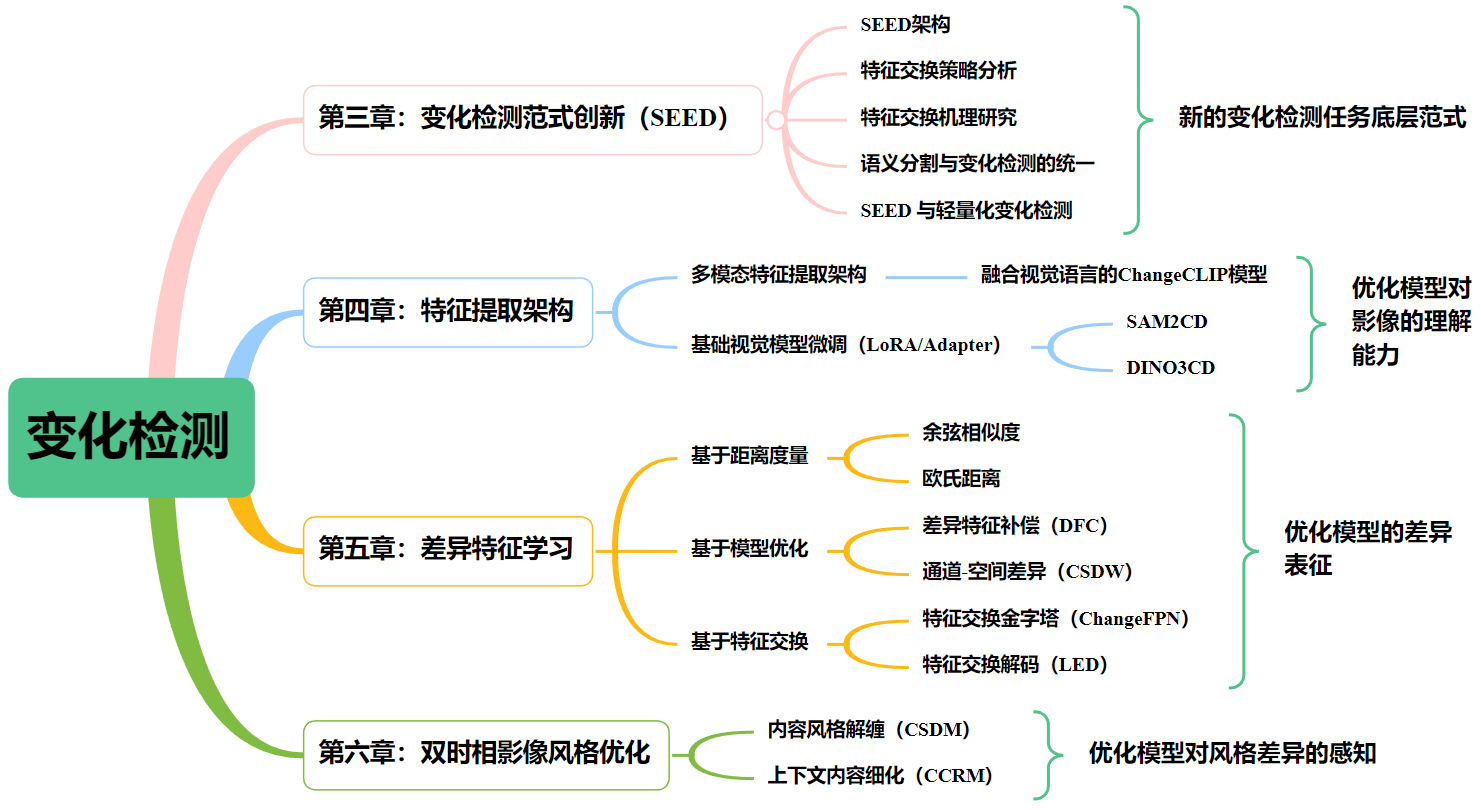
\includegraphics[width=\textwidth]{paper_figures/绪论/研究内容关联.png}
  \caption{研究内容及其关联性}
  \label{fig:research_content}
\end{figure}


\section{研究内容及其关联性}
本文主要聚焦于基于特征交换的高分辨率遥感影像变化检测方法的创新与优化。对于常规的计算机视觉任务而言,通常有如下的研究方向,首先是加强模型的特征提取能力,构建更强大的特征提取架构,增强模型的特征拟合能力,比如VGG~\cite{Simonyan2014VeryDC}、ResNet~\cite{He2015DeepRL}以及ViT~\cite{Dosovitskiy2020AnII}等骨架模型。其次是针对具体的视觉任务,设计加强特征学习能力的模块,比如DeeplabV3plus~\cite{chen2018encoder}、PSPNet~\cite{Zhao2016PyramidSP}以及EMANet~\cite{Li2019ExpectationMaximizationAN}等模型。此外也可以根据具体的视觉任务,设计全新的模型架构,比如FCN~\cite{Shelhamer2014FullyCN}、UNet~\cite{Ronneberger2015UNetCN}以及SETR~\cite{Zheng2020RethinkingSS}等模型。根据上述常规的计算机视觉算法优化研究思路,本文在变化检测任务上围绕上述的思路进行了研究,如图~\ref{fig:research_content}所示。针对变化检测任务,本文从\textbf{变化检测架构设计优化变化检测模型对变化特征的表征方式}、\textbf{特征提取强化提升变化检测模型的对双时相影像的表征能力}、\textbf{双时相特征交互优化变化检测模型对差异特征的学习能力}以及\textbf{双时相影像风格优化减弱变化检测任务风格噪声的影响}四个方面展开了研究。

\subsection{变化检测范式创新}
现有多数变化检测架构沿用“孪生编码—差异计算—解码”的范式,其核心在于显式构造差异特征。不同于此,本文提出孪生-编码-交换-解码(\textbf{Siamese-Encoder-Exchange-Decoder,SEED})基础架构:在共享权重的孪生编码器提取出双时相多尺度特征金字塔后,\textbf{不进行任何显式差分运算},而是于进入解码阶段前执行\textbf{特征交换}(可采用特征层、空间以及通道交换),使两个孪生解码器均接收由\(T_1\)与\(T_2\)混合而成的特征序列,并使用同一变化标注进行监督。该设计将“变化”的定义由手工设定的差异特征学习,转化为模型对\textbf{双时相特征不一致性}的\textbf{隐式判别}。未变化区域在交换后的解码端保持语义—空间一致,则在模型学习中被判别为背景区域。而发生变化的区域在解码端呈现双时相影像特征的语义冲突,从而被网络自适应分割出来。SEED舍弃显式差异计算模块,结构更为简洁、参数与计算更友好,同时避免了固定运算(如相减/拼接)可能带来的信息损失,充分发挥深层网络在端到端学习\textbf{一致性/不一致性}判别上的优势。综上,此部分从理论和实验上证明了特征交换策略在变化检测任务中的有效性,为后文的模型优化奠定了基础。

\subsection{基于 AI 基础模型的变化检测特征提取强化}
针对变化检测中单一模态语义先验不足、模型泛化受限的问题,本文从\textbf{多模态视觉—语言}与\textbf{基础模型参数高效适配}两条路径强化特征提取能力。一方面,本文构建基于CLIP模型的多模态特征提取范式:利用CLIP对双时相遥感影像进行无监督语义推理,生成类别相关的文本提示,并在编码—解码框架中通过低秩双线性注意力将图像特征与文本特征进行融合,从而显式补充遥感影像的\textbf{语义信息},提升模型对复杂遥感影像的辨识能力。另一方面,面向SAM与DINO等视觉基础模型,本文提出结合视觉基础模型参数高效微调(PEFT)策略的变化检测模型PeftCD。在冻结预训练参数的前提下,通过LoRA/Adapter轻量化微调分支注入任务相关表征,有效保留大规模预训练的通用先验并使得模型充分学习到遥感影像相关知识。其中,PeftCD在变化检测范式上采用SEED架构,以此验证了SEED架构的有效性。综上,本文以\textbf{“多模态语义注入+视觉基础模型PEFT适配”}两条路径协同强化特征提取,有效缓解了单一模态语义先验不足与传统视觉模型泛化受限的问题。

\subsection{基于双时相特征交互的差异特征学习}
通常认在变化检测任务中,双时相特征交互是指利用双时相影像提取的特征,通过某种计算方法提取出能表征双时相影像差异的步骤。因此,双时相特征交互是由输入对迈向“学习变化表征”的关键步骤,。本文从互补的三个维度开展设计:(i)\textbf{差异特征计算}:围绕“如何更准确的表达双时相特征的差异”,本文在简单运算(差/和/拼接)之上,提出了基于距离度量方式(欧氏距离、余弦相似度距离)的差异特征学习模块;(ii)\textbf{结合模型设计的差异特征表达方法}: 围绕如何使用网络模块来更好的表达双时相特征的差异性,本文提出了结合空间和通道差异的差异表征方法,将变化检测任务中普遍存在的空间差异特征拓展到了空间-通道相结合的差异特征。(iii)\textbf{特征交换机制}:基于双时相影像\textbf{同地理位置}的先验,设计了基于特征层的双时相影像特征交换策略,在不显式施加差分约束的前提下,促进两时相特征的信息相互流动,使\textbf{语义不一致性}在双时相混合表征中自发显现。这三类机制分别从“显式度量差异”、“模型拟合差异”和“隐式表征差异”出发,在训练时以同一变化监督进行统一优化。

\subsection{双时相影像内容风格解缠}

针对双时相遥感影像因光照、季节等因素造成的风格差异(域偏移)干扰变化检测精度的问题,本文提出了一种基于内容-风格解耦与内容细化的变化检测网络(Content Style Disentanglement Network,CSDNet)。该模型显式分离内容特征与风格特征,并利用门控机制对风格信息进行自适应筛选,在有效抑制无关噪声的同时保留对变化判别有益的纹理等细节。具体而言,CSDNet首先通过内容-风格解缠模块(CSDM)将双时相影像特征分解为内容特征和风格特征。然后,设计了通道-空间门控机制(CSGM)对风格特征进行动态筛选,抑制无关风格信息并保留有助于变化识别的细节。最后,将筛选后的风格特征与内容特征融合,生成更鲁棒的变化表征。通过这种方式,CSDNet有效减弱了风格差异对变化检测的干扰,提高了模型在复杂场景下的精度和泛化能力。此外,本文提出的CSDNet同样采用SEED架构,再次验证了SEED架构在复变化检测任务中的有效性。

\begin{figure}[!htbp]
  \centering
  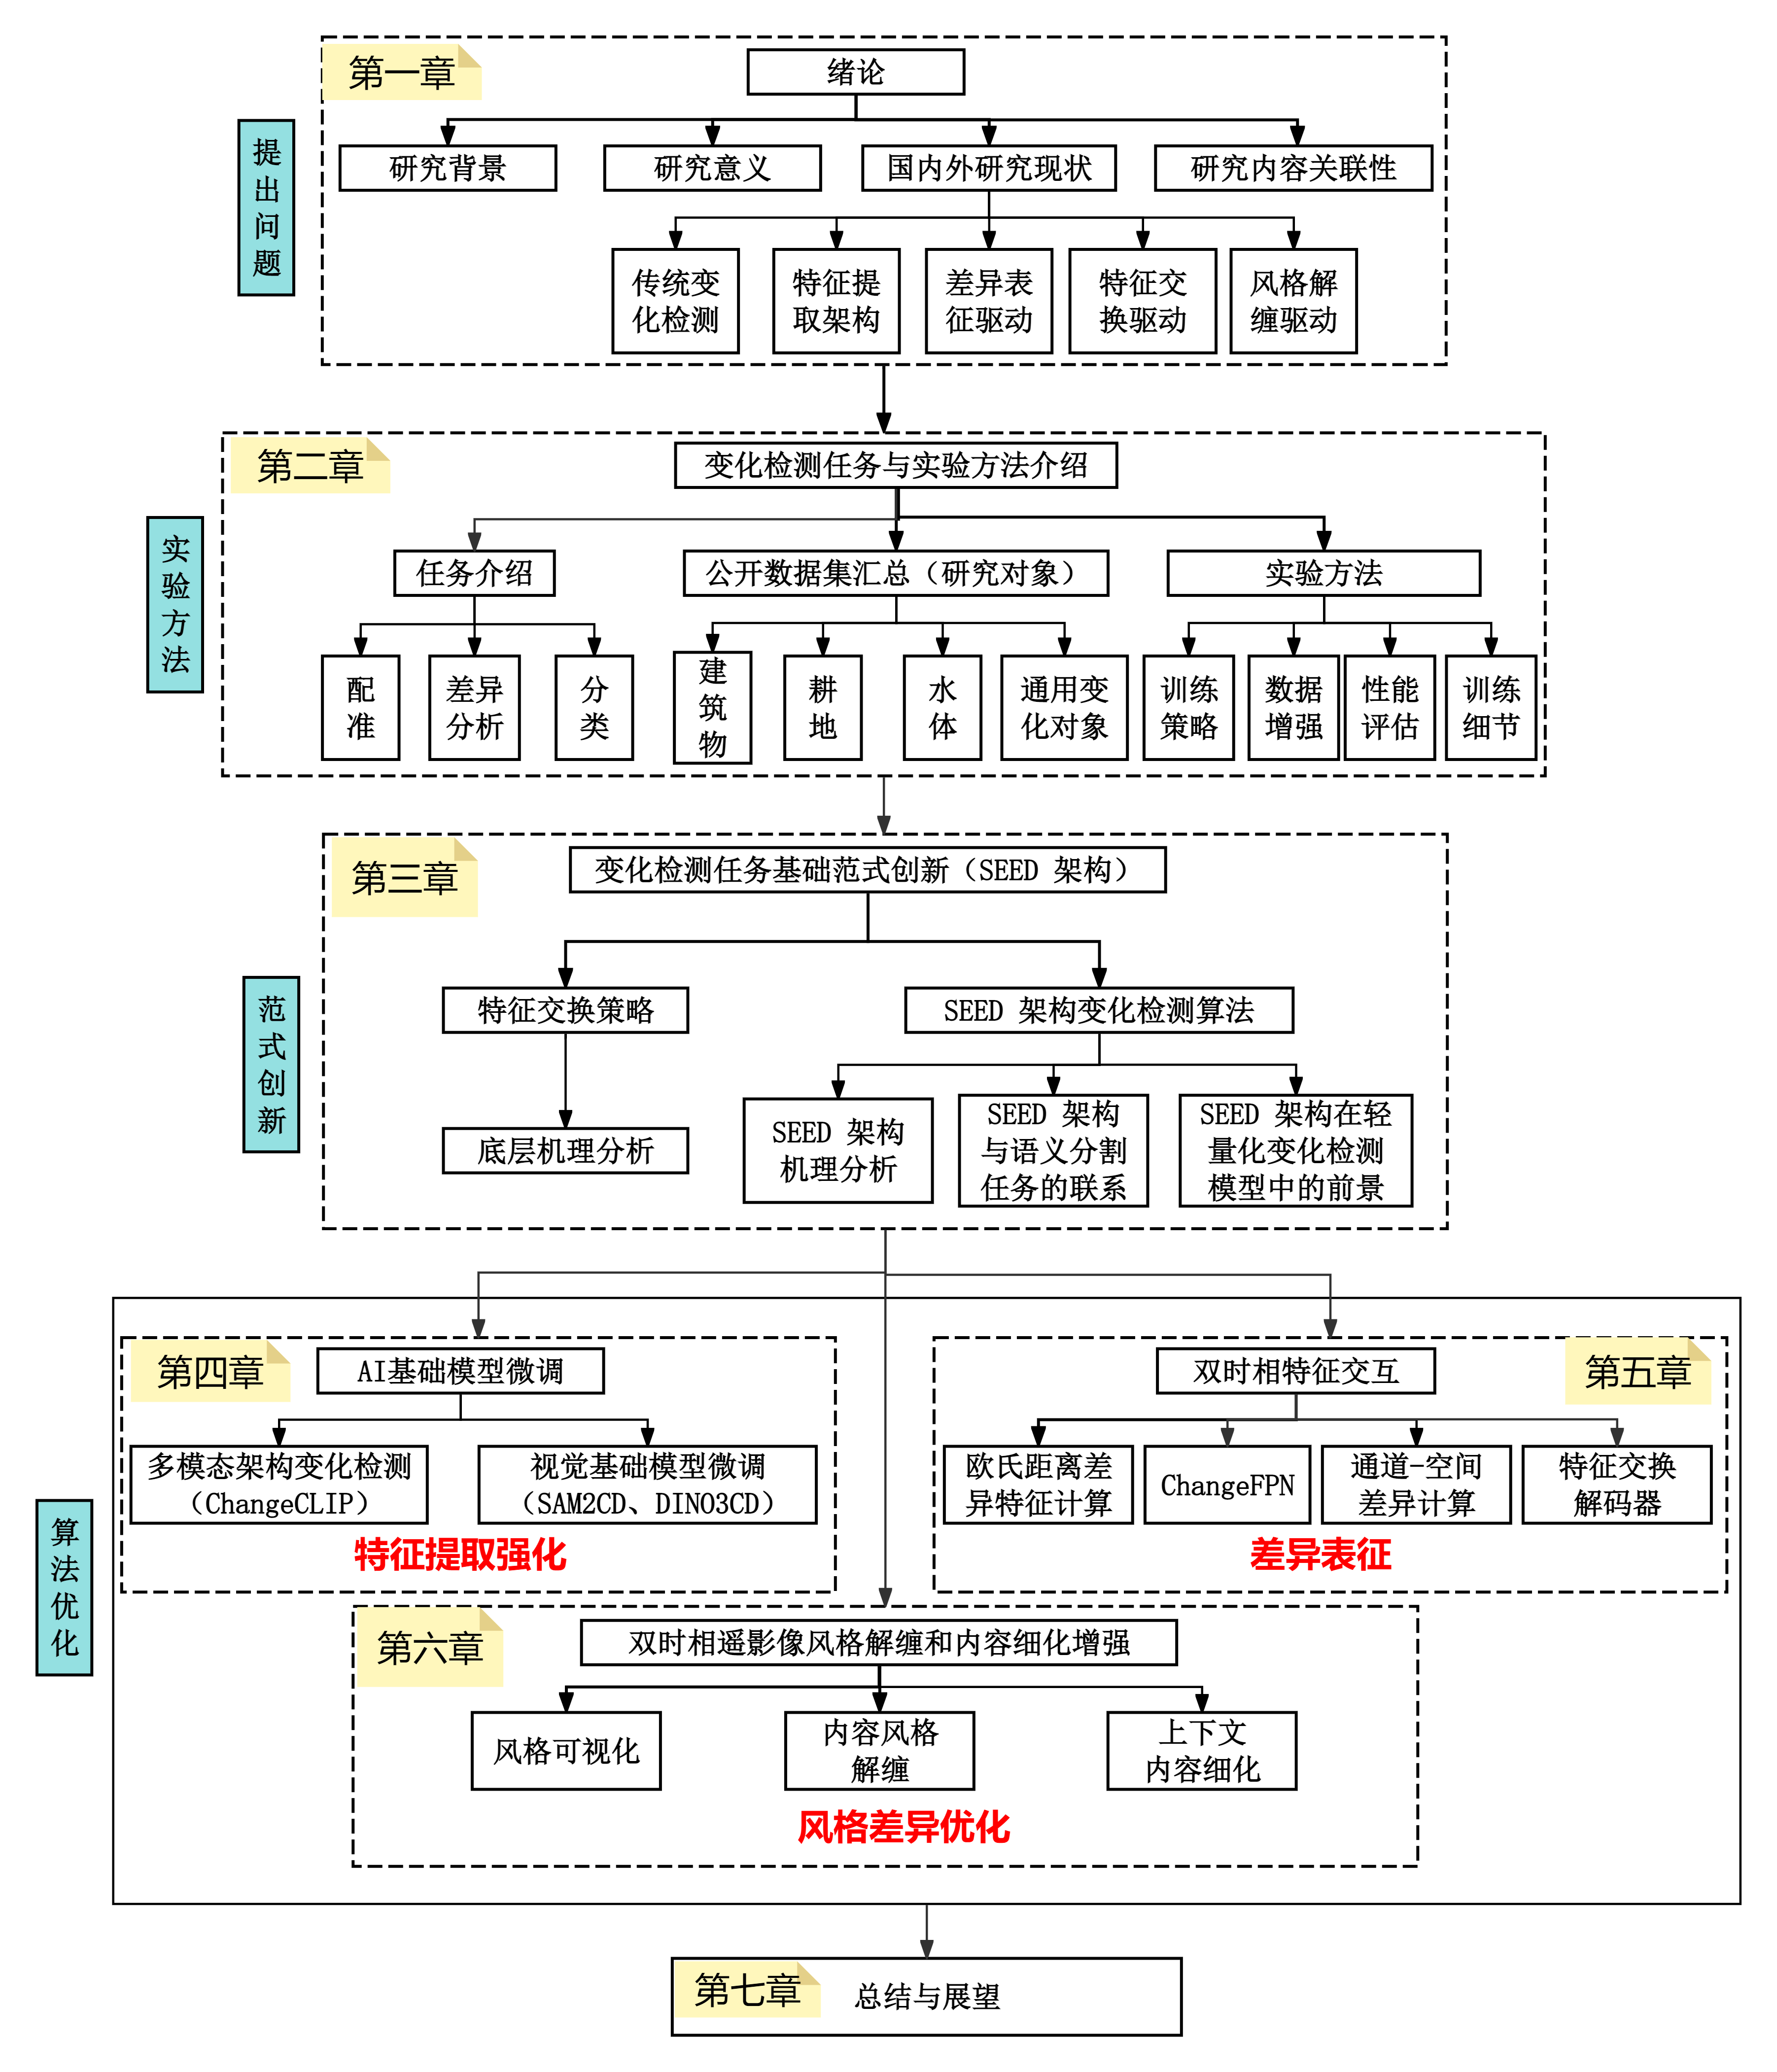
\includegraphics[width=\textwidth]{paper_figures/绪论/论文章节技术路线图.png}
  \caption{论文技术路线}
  \label{fig:paper_overall}
\end{figure}

\section{论文组织结构}
综上,本文的技术路线如图~\ref{fig:paper_overall}所示,整体分为四个层面逐步展开。首先,在绪论部分明确研究背景、意义及国内外研究现状,提出高分辨率遥感影像变化检测中存在的关键问题。其次,在实验方法部分,介绍了变化检测任务的具体实验方法。包括本文使用的多种类的数据集以及实验条件,为后文的算法设计提供了基础。随后,针对于变化检测任务范式创新,提出了Siamese-Encoder-Exchange-Decoder (SEED) 框架,以特征交换为核心机制,突破传统依赖显式差异计算的模式,实现了对变化检测任务的新型范式重构。后文的部分模型围绕SEED架构进行设计,由此证明了SEED架构的有效性。接着,本文从特征提取强化、双时相特征交互以及伪变化抑制三个方面对变化检测任务进行算法优化。在特征提取部分,论文围绕如何提升模型的特征提取能力展开,提出了基于AI基础模型微调的ChangeCLIP和PeftCD模型。在双时相特征交互部分,论文围绕如何更好的表征双时相影像的差异性展开,提出了基于距离度量的EfficientCD以及融合了通道与空间维度的(Layer-Exchange Network,LENet)。在伪变化抑制部分,论文围绕如何减弱风格噪声对变化检测任务的影响展开,提出了基于内容-风格解缠与内容细化的CSDNet模型。在此基础上,论文通过总结与展望进一步指出未来在多模态融合、跨域泛化及大规模基础模型适配等方向的研究潜力。本文的各个章节安排如下:

\textbf{第一章,绪论}。 本章首先阐述了高分辨率遥感影像变化检测的研究背景、重要意义以及当前面临的关键挑战。随后,系统回顾了变化检测算法的发展历程,涵盖了变化检测特征提取架构从传统方法到深度学习中CNN、Transformer、Mamba及AI基础模型的演进。在此基础上,进一步剖析了以差异表征和特征交换为核心的两种主流技术路线。最后,明确了本文的研究内容、核心贡献与总体技术框架,并概述了全文的组织结构。

\textbf{第二章,变化检测任务与实验方法介绍}。 本章为后续的算法研究与验证奠定基础。首先,详细介绍了本文实验所采用的多个公开变化检测数据集,涵盖了建筑物、农田、水体及通用场景等多种变化类型。接着,系统阐述了变化检测的标准实验流程,包括模型训练策略、数据增强技术以及精度验证所使用的各项性能评估指标。

\textbf{第三章,基于特征交换的变化检测基础范式创新设计}。 本章提出了一个颠覆性的变化检测基础架构——SEED (Siamese-Encoder-Exchange-Decoder)。该范式摒弃了传统的差异特征计算模块,仅通过特征交换来驱动模型学习双时相特征的不一致性。本章深入探讨了该范式背后的“像素一致性原则”,并通过实验证明了其在简化模型设计、变化检测轻量化架构、统一变化检测与语义分割任务方面的巨大潜力和卓越性能。此外,本章针对变化检测特征交换的理论和实验证明,为后续模型设计提供了坚实的理论和实验基础。

\textbf{第四章,基于AI基础模型微调的变化检测模型研究}。 本章聚焦于利用AI基础模型的强大先验知识来强化变化检测的特征提取能力。内容分为两个核心部分:第一部分介绍ChangeCLIP模型,探索了将多模态视觉-语言模型(CLIP)引入变化检测任务的方法;第二部分介绍PeftCD模型,研究了如何通过参数高效微调(PEFT)技术,将多种视觉基础模型高效适配于遥感变化检测场景,并对不同基础模型的性能进行了系统性比较。

\textbf{第五章,基于双时相遥感影像特征交互的变化检测算法研究}。 本章重点研究以“差异表征”为核心的双时相特征交互机制。内容涵盖了多种创新的差异特征计算模块,包括基于交互注意力机制的ISANet、基于距离度量的EfficientCD以及融合了通道与空间维度的LENet。通过详尽的对比实验与消融分析,验证了这些差异学习策略在提升模型对复杂变化感知能力方面的有效性。

\textbf{第六章,基于双时相遥感影像风格解缠和内容细化增强遥感变化检测方法}。 本章针对双时相遥感影像间因光照、季节等因素造成的风格差异(域偏移)干扰变化检测精度的问题,提出了一种基于内容-风格解耦与内容细化的变化检测网络(CSDNet)。该模型显式分离内容特征与风格特征,并利用门控机制对风格信息进行自适应筛选,在有效抑制无关噪声的同时保留对变化判别有益的纹理等细节。

\textbf{第七章,总结与展望}。 本章对全文的研究工作进行了全面总结,系统回顾了本文在变化检测领域的理论创新与主要贡献。在此基础上,对未来可能的研究方向进行了展望,指出了多模态融合、自监督学习、模型可解释性等领域的潜在突破口。
% 
\chapter{变化检测任务与实验方法介绍}
遥感影像变化检测(Remote Sensing Change Detection, RSCD)是遥感技术中的一个重要应用,旨在通过对比两幅或多幅在不同时间拍摄的遥感影像,识别出地表的变化区域~\cite{YGXB202407012}。随着遥感技术的进步和深度学习技术的应用,变化检测任务已经逐渐从传统的像素差异法、图像配准方法,发展为基于深度神经网络的方法。这些方法能够更准确地从遥感影像中提取特征,识别变化区域,尤其是在复杂背景和微小变化的情况下。

\section{变化检测任务介绍}

变化检测任务的核心目标是识别在不同时间点拍摄的两幅或多幅遥感影像之间的差异。这一任务对于环境监测、灾害评估、城市扩展检测、资源管理等多个领域具有重要意义。传统的变化检测方法主要依赖于像素级别的差异分析,而随着深度学习技术的引入,基于深度神经网络的变化检测方法通过自动学习多层次特征和复杂模式,显著提高了变化检测的精度和鲁棒性。

在目前普遍应用的基于深度学习的变化检测任务中,通常涉及到以下几个关键任务:

\textbf{双时相影像配准}:由于双时相的遥感影像在获取过程中可能存在拍摄时间、传感器类型及成像角度等方面的差异,图像配准成为变化检测的前提~\cite{WHCH202405001}。高精度的配准能够保证双时相影像在空间位置上的一致性,从而为后续的差异分析和变化识别提供可靠基础。同时,双时相影像在空间位置上的一致性,也是普遍的全监督变化检测任务能够成功进行的前提。配准方法通常包括基于特征点的配准、基于图像块的配准以及基于深度学习的配准等~\cite{YGXB202406011}。

\textbf{双时相影像差异特征分析}:在遥感影像变化检测任务中,双时相影像差异特征分析是至关重要的一步~\cite{CHXB202207001}。传统的差异计算方法通常依赖于像素级别的对比,如直接相减或计算变化指数。然而,随着深度学习技术的引入,基于神经网络的方法可以自动学习影像中的深层次特征,从而更准确地捕捉图像中的微小变化。在深度学习框架下,差异特征计算主要依赖于模型通过训练学习到的高级视觉特征。通过卷积神经网络(CNN)或其他深度学习模型提取双时相影像的多层次特征后,网络能够学习到不同时间点影像之间的差异性~\cite{chen_spatial-temporal_2020,lin_transition_2023,shi_deeply_2022}。这种方法不仅能够识别明显的变化区域,还能够识别由于地形变化、光照变化等因素导致的微小变化。

\textbf{变化区域识别与分类}:在变化区域的分类过程中,深度神经网络能够通过对比不同时间点的影像特征,自动学习变化与不变化区域的区分方法。对于不同的变化类型(如建筑物、新建道路、植被变化等),模型可以进一步将变化区域进行细化分类。通常,变化检测任务在变化区域的分类上与语义分割任务类似,均是利用神经网络进行像素级的分类任务。这些网络结构通过编码器-解码器的架构,可以在编码阶段提取高层次的特征表示,并通过解码阶段逐步恢复图像的空间分辨率,从而实现精细的像素级预测。然而,与侧重于单幅影像空间语义理解的语义分割不同,变化检测的核心目标是识别目标语义类别是否发生变化,而非仅仅是识别静态的语义类别本身,这对其特征提取和差异判别能力提出了更高的要求。在变化检测任务中,网络通过学习图像的时空特征差异,能够自动识别出哪些区域发生了变化,并将变化区域与不变区域区分开来。 

除此之外,为了系统性地评测和比较不同变化检测算法在上述关键环节中的性能,并推动算法向更高精度、更强鲁棒性的方向发展,相关研究人员构建了一系列公开的变化检测任务基准数据集。这些数据集的多样性和挑战性,为算法的有效性验证和泛化能力分析提供了重要的实验基础。

\section{常用的变化检测数据集介绍}
遥感影像变化检测的研究依赖于大量的实验数据集。为了证明本文本在变化检测任务的研究的广泛性和深刻性,本文选用了多种不同数据偏重的变化检测数据集来进行实验。这些数据集涵盖了不同的地理区域、变化类型以及影像质量,从而确保实验结果的广泛适用性。数据集包括了城市区域、农业区域、自然环境、海洋周边区域等多种场景,涉及建筑物变化、农田变化、水体变化等多种变化类型。这些数据集的多样性使得能够从多个角度对变化检测算法进行深入分析,探讨其在不同场景下的表现和局限性。具体而言,这些数据集分别在变化尺度、目标密度、背景复杂性、以及由季节和光照引起的伪变化等方面构成了不同的挑战,从而能够全面地检验变化检测算法的综合性能。

\subsection{针对建筑物区域的变化检测数据集}
\subsubsection{LEVIR-CD与LEVIR-CD+数据集}
LEVIR-CD~\cite{chen_spatial-temporal_2020}是一个大规模的遥感建筑变化检测数据集,旨在为变化检测(CD)算法,特别是基于深度学习的算法,提供一个新的评估基准。该数据集包含637对高分辨率(0.5m/像素)的Google Earth图像块,其中445对训练样本,64对验证样本,128对测试样本。每个图像块的大小为1024 × 1024像素,图像覆盖的时间跨度为5至14年,具有显著的土地利用变化,特别是建筑增长。如图~\ref{fig:levir_cd}所示,LEVIR-CD数据集重点关注与建筑物相关的变化,包括建筑物增长(从土壤、草地或建设中的建筑转变为新的建筑区域)和建筑物的减少。每对图像都由遥感图像解说专家进行二进制标签注释,最终提供了31,333个单独的建筑变化实例。数据集的地理空间分布包括美国德克萨斯州的多个城市,图像采集时间从2002年到2018年不等。由于不同区域的图像拍摄时间存在差异,该数据集引入了季节变化和光照变化的影响,这将有助于开发能够缓解这些不相关变化对实际变化影响的有效方法。LEVIR-CD数据集的构建提供了一个高质量的基准,具有丰富的建筑物变化实例,是建筑物变化检测任务中最常用的开源数据集之一。如图~\ref{fig:levir_cd_plus}所示, LEVIR-CD+~\cite{chen_spatial-temporal_2020}数据集是LEVIR-CD的扩展版本,包含985对遥感图像,其中637对属于训练数据集,其余的用于测试。

\begin{figure}[!htbp]
  \centering
  \includegraphics[width=0.75\textwidth]{paper_figures/变化检测任务与实验方法介绍/levir_cd.png}
  \caption{LEVIR-CD 数据集展示.}
  \label{fig:levir_cd}
\end{figure}

\begin{figure}[!htbp]
  \centering
  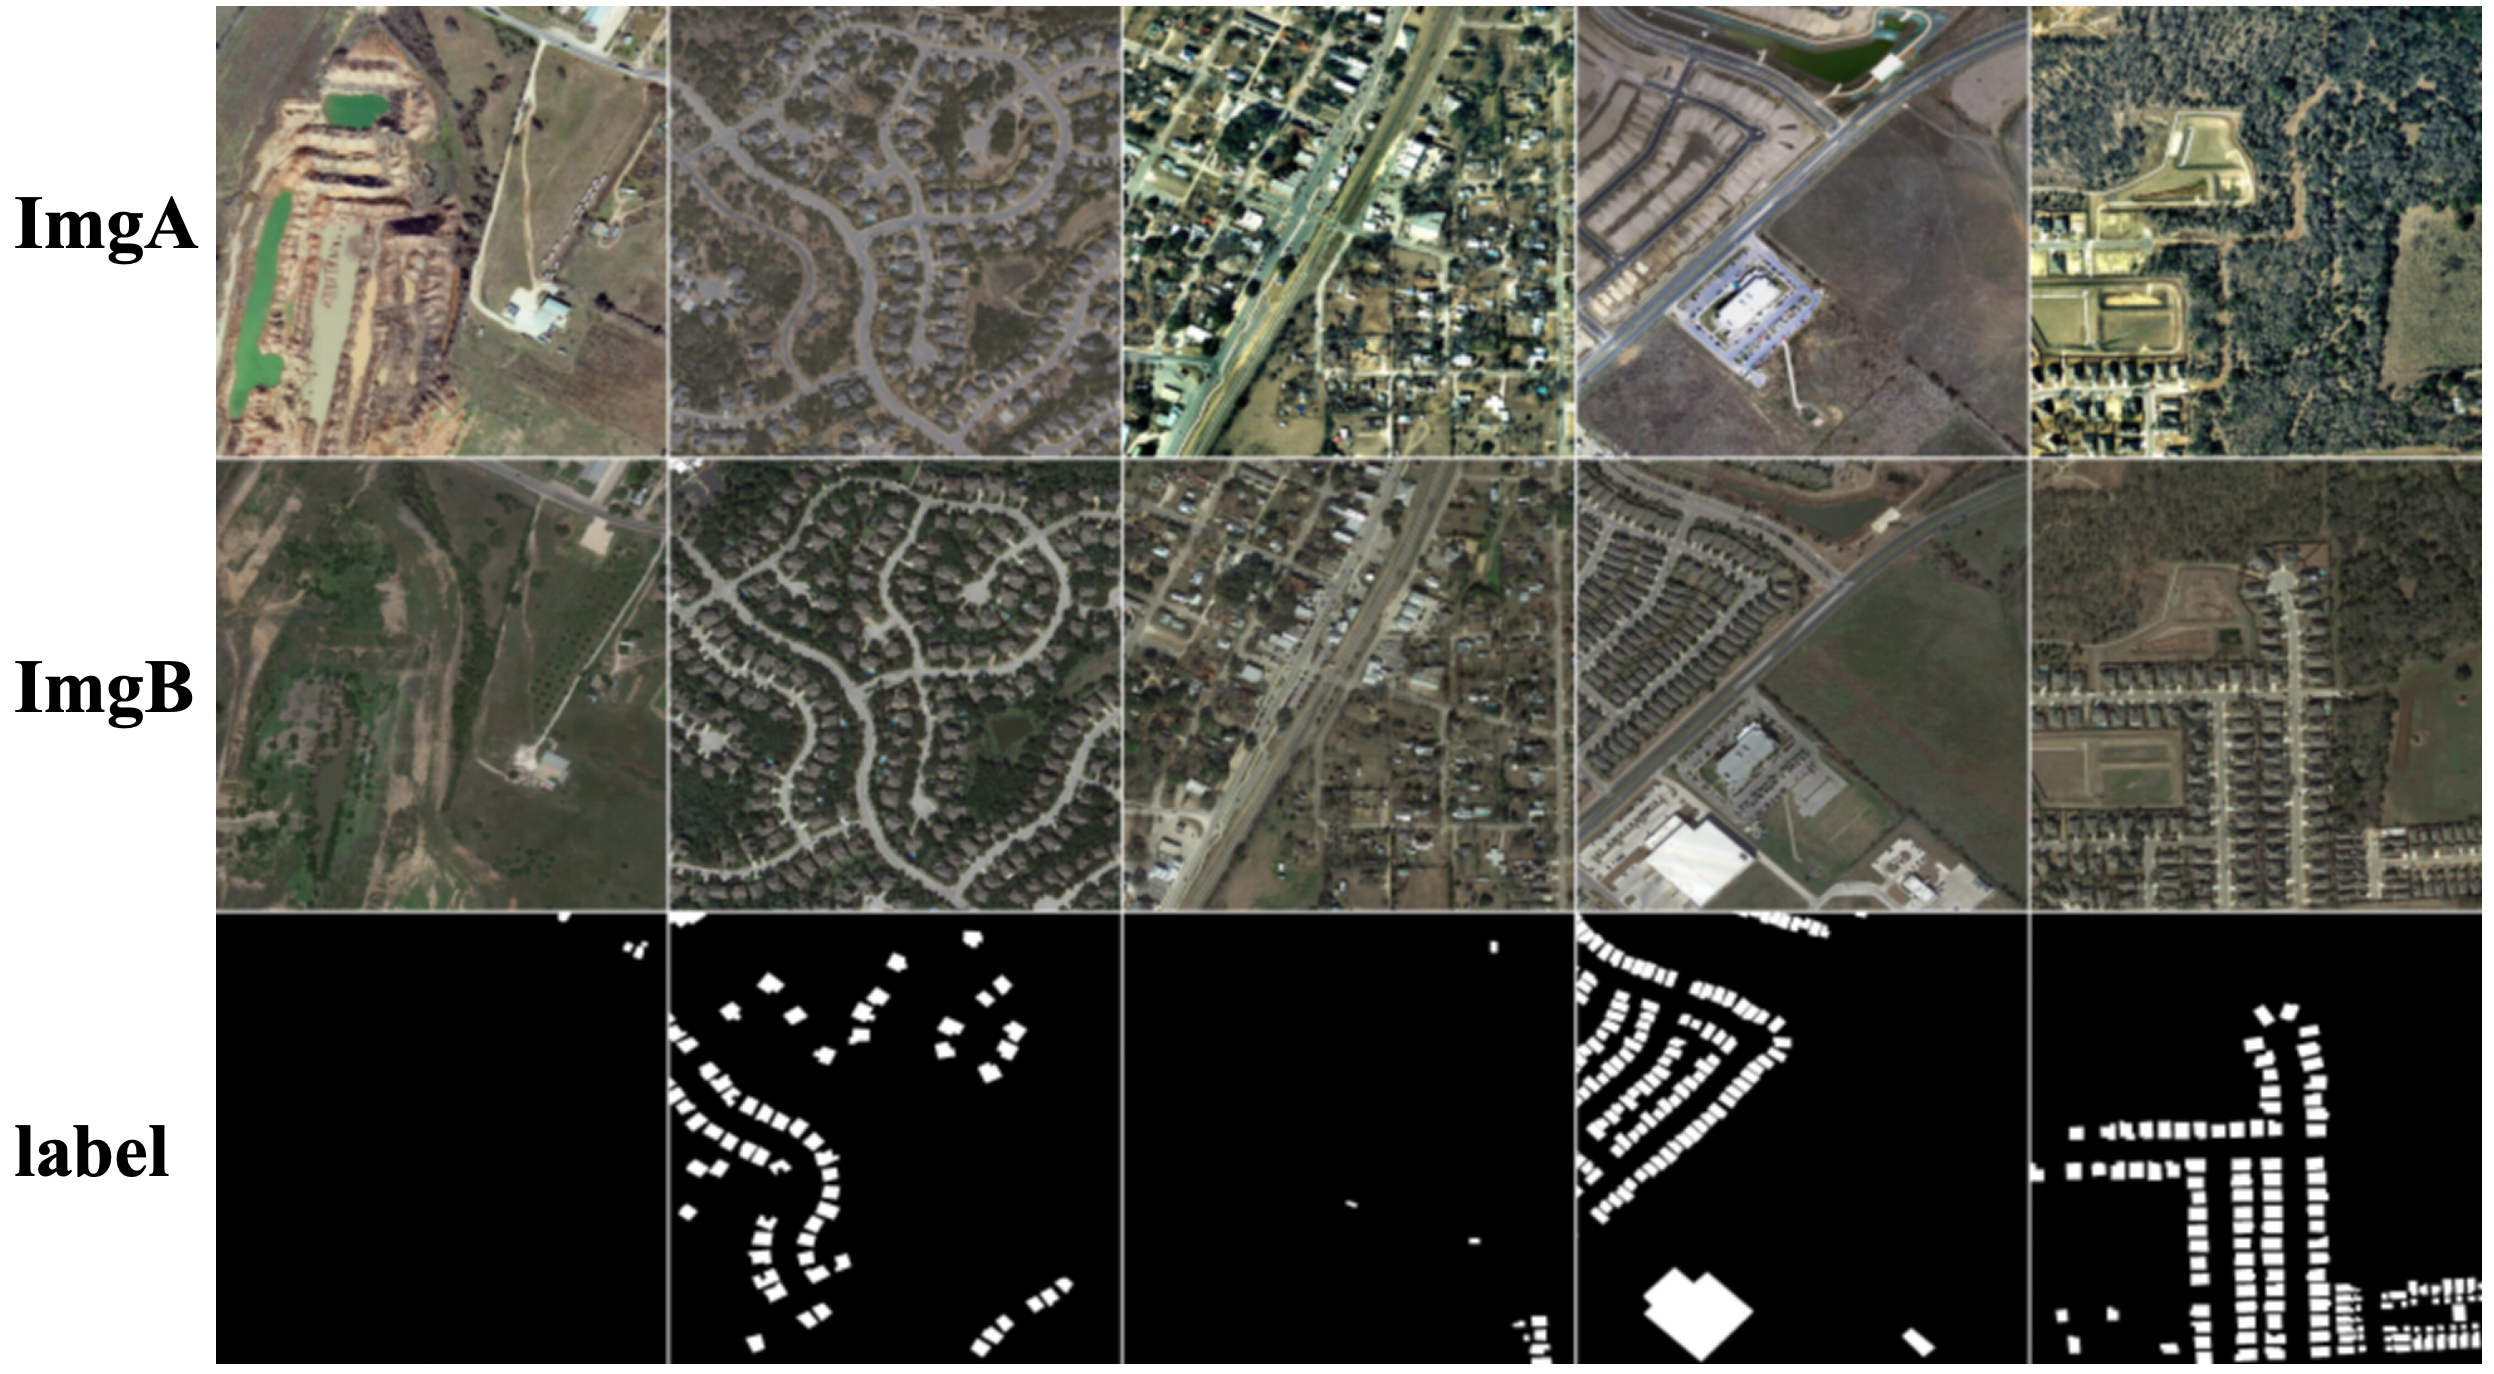
\includegraphics[width=0.75\textwidth]{paper_figures/变化检测任务与实验方法介绍/levir_cd_plus.png}
  \caption{LEVIR-CD+ 数据集展示.}
  \label{fig:levir_cd_plus}
\end{figure}

\subsubsection{S2Looking数据集}
S2Looking数据集~\cite{Shen2021S2LookingAS}是为推动建筑物变化检测研究而创建的,提供了一个新的、更具挑战性的资源。与LEVIR-CD+数据集相比,S2Looking扩展了数据集的规模,涵盖了农村地区的侧视遥感图像。由于其特殊的图像角度,S2Looking数据集所面临的变化检测问题与传统的基于Google Earth图像的数据集有所不同。数据集中包含了大量的建筑物增长和衰退的变化,但由于农村地区建筑物更新的稀疏性,这些变化的检测更具挑战性,如图~\ref{fig:s2looking}所示。

S2Looking数据集的一个显著特点是建筑变化实例的稀疏性。农村地区大多覆盖农田和森林,建筑物较为稀少,而城市地区则是建筑物密集、不断变化的区域。S2Looking中的变化实例数量较少,平均为13.184个,而LEVIR-CD中的变化实例为49.188个。这使得在进行建筑特征提取时,网络需要更好地适应稀疏数据和复杂背景。此外,S2Looking数据集采用侧视遥感图像,建筑物的影像是由卫星从不同的角度拍摄并投影成二维图像,这使得变化检测模型需要能够识别从不同角度拍摄的同一建筑物并检测其变化。由于农村地区季节性变化和与建筑更新无关的土地覆盖变化更加明显,S2Looking数据集面临着更为复杂的环境。农田的季节性变化和不同作物的覆盖使得土地在遥感图像中呈现不同的外观。因此,适用于此数据集的变化检测模型必须能够区分建筑变化与这些无关变化,以减少误检。

\begin{figure}[!htbp]
  \centering
  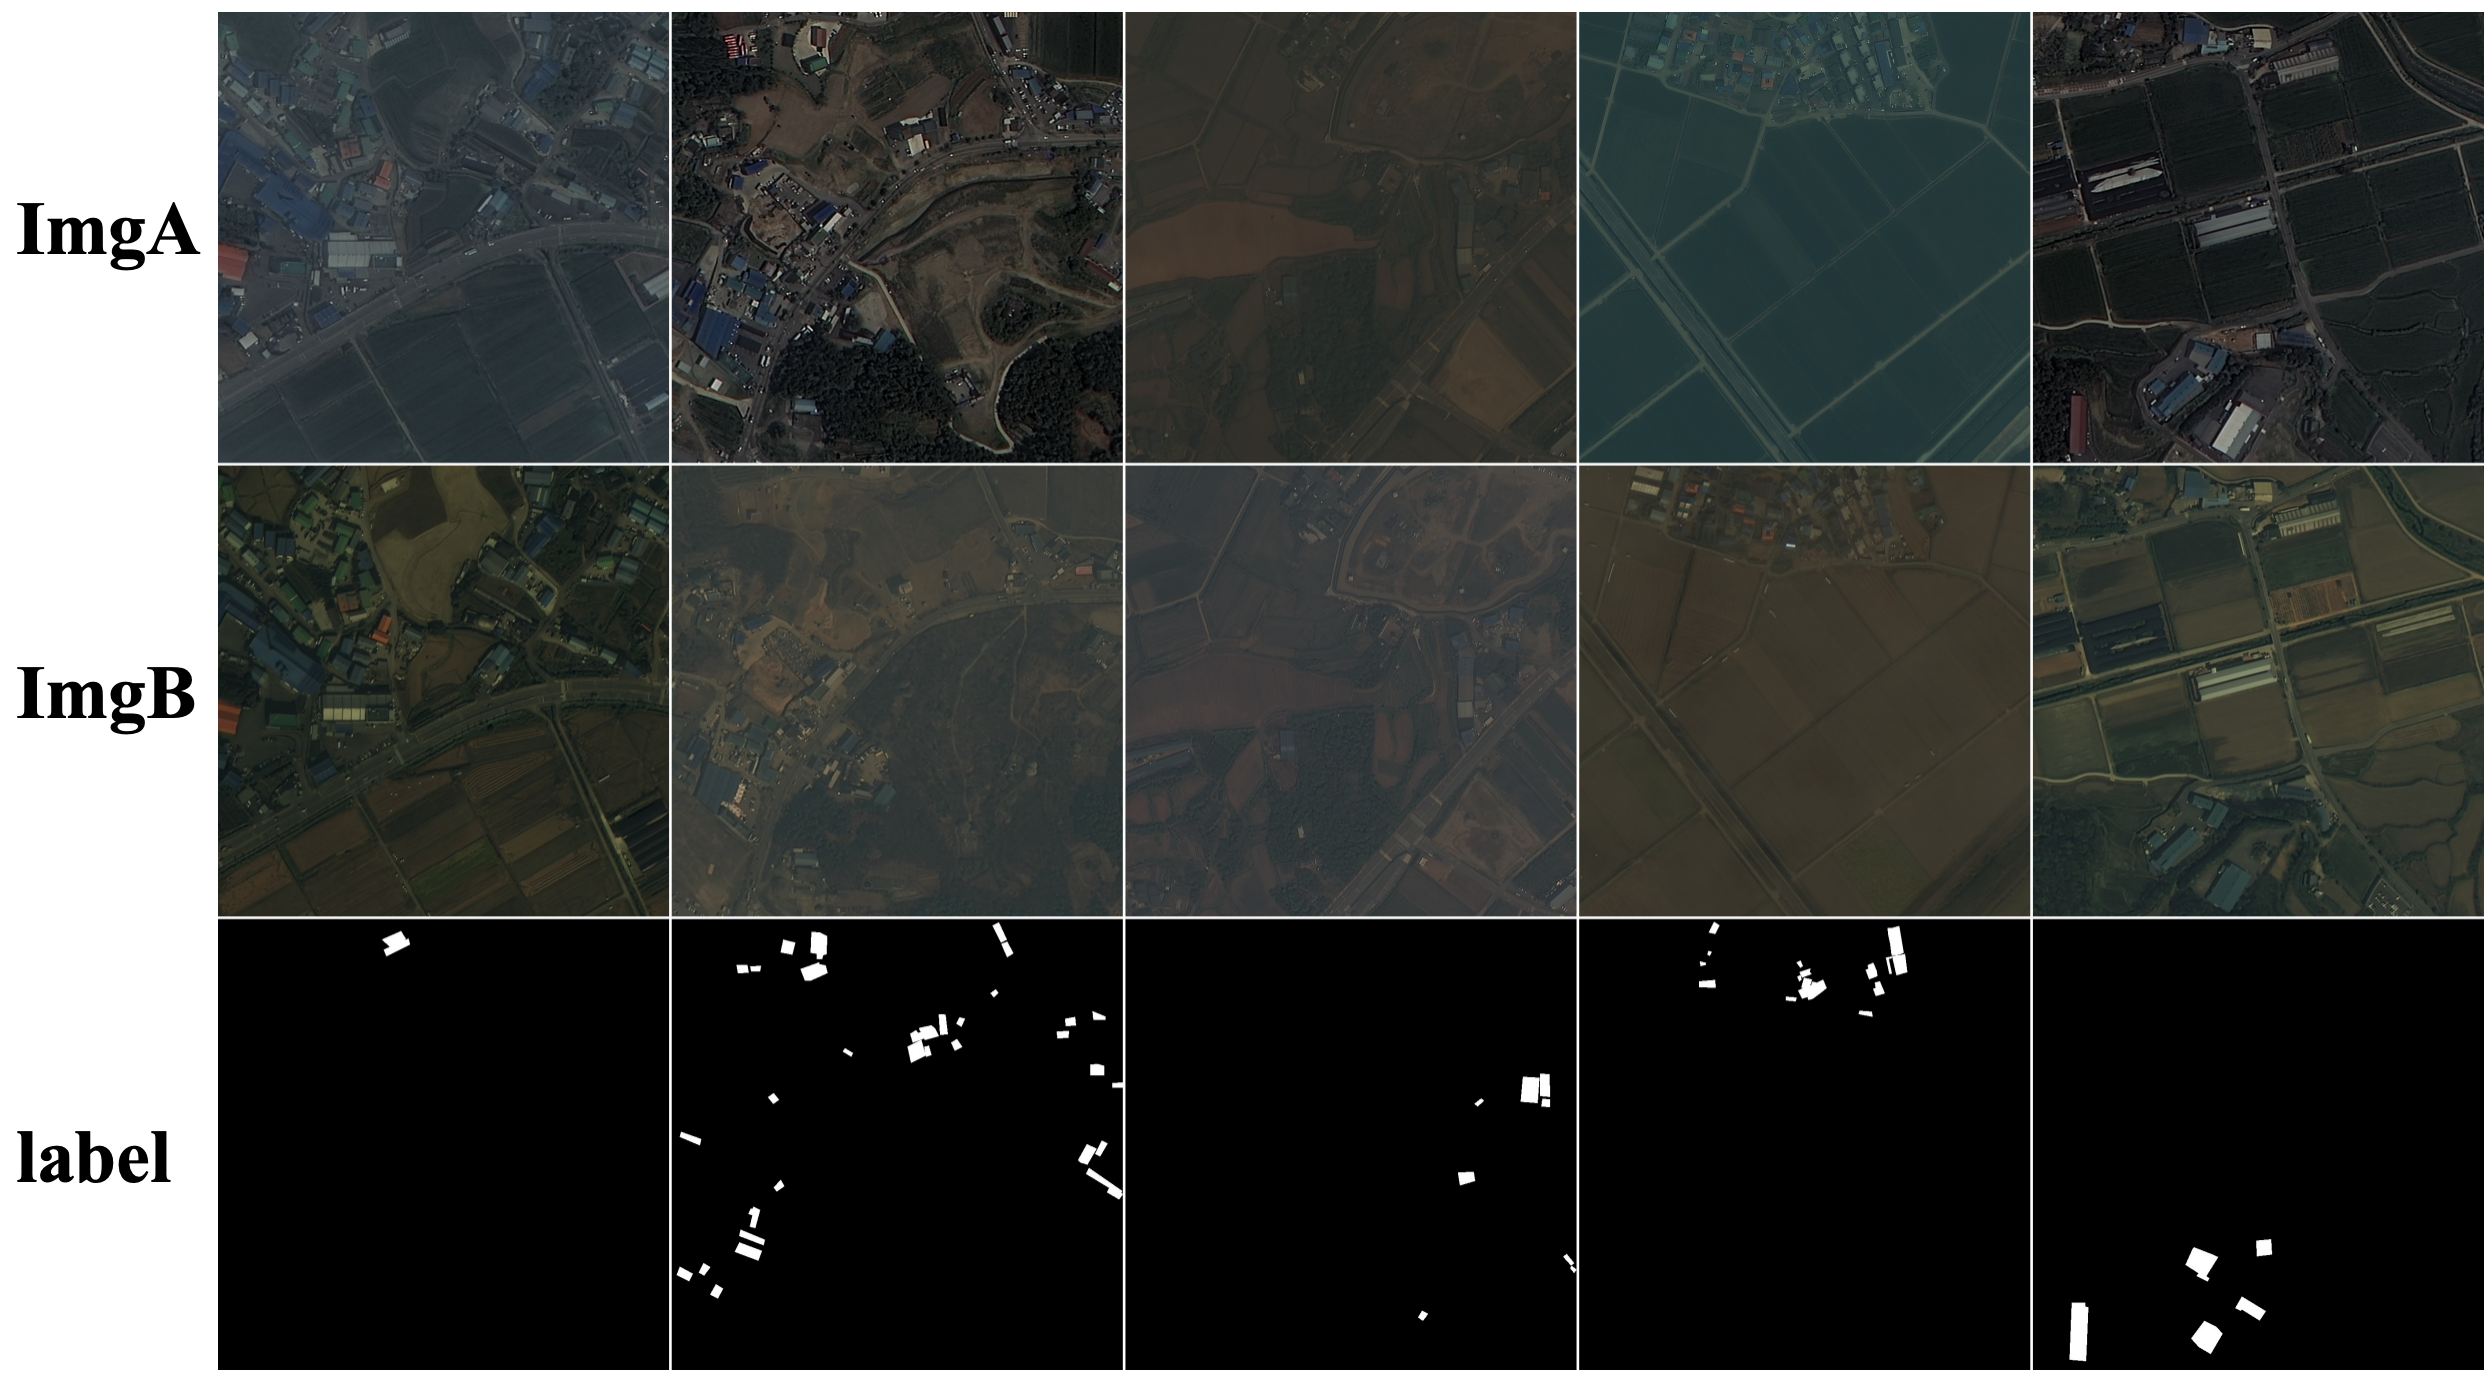
\includegraphics[width=0.75\textwidth]{paper_figures/变化检测任务与实验方法介绍/s2looking.png}
  \caption{S2Looking 数据集展示.}
  \label{fig:s2looking}
\end{figure}


\subsubsection{WHUCD数据集}
WHU建筑物数据集~\cite{Ji2019FullyCN}是一个由航拍图像和卫星图像构成的建筑物样本数据集,旨在为建筑物提取和变化检测研究提供重要的数据支持。该数据集包含超过220,000座独立建筑物,其中航拍数据集来自新西兰基督城,图像的空间分辨率为0.075米,覆盖面积达到450平方公里。在WHUCD的实验中,对原始的大尺寸影像进行裁剪,按照$256 \times 256$大小进行切分,如图~\ref{fig:whucd}所示。最终按照8:1:1的比例,得到6096张训练集图片,762张验证集图片,以及762张测试集图片。


\begin{figure}[!htbp]
  \centering
  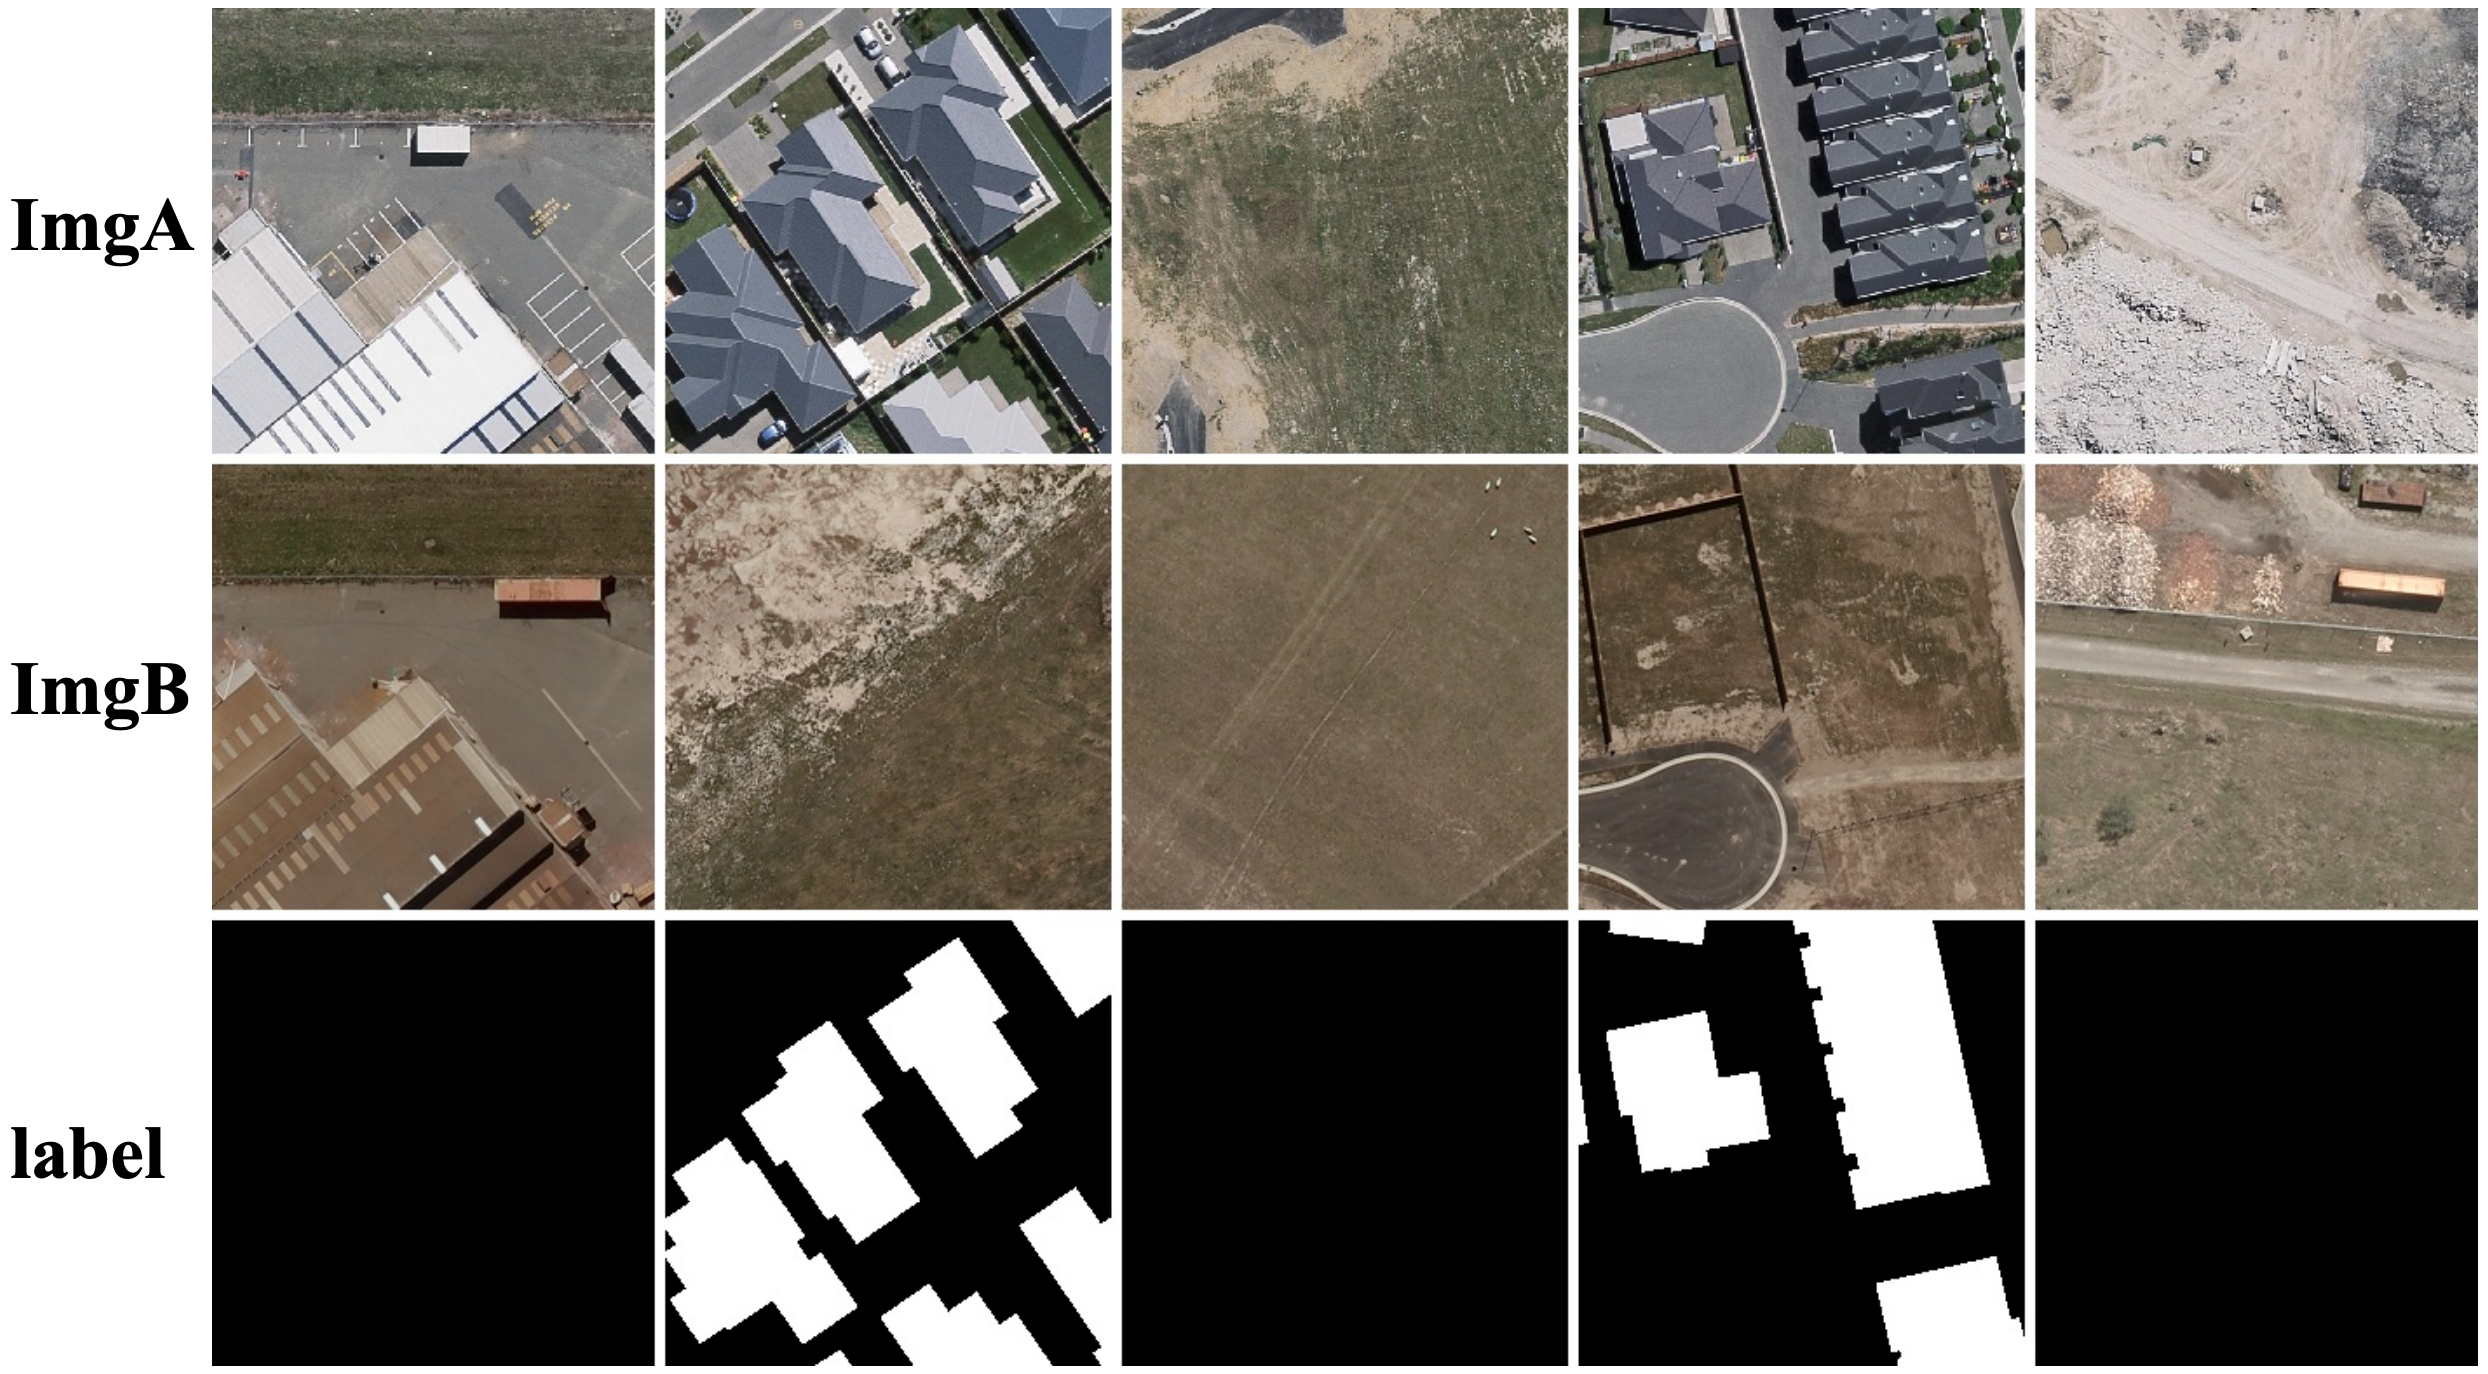
\includegraphics[width=0.75\textwidth]{paper_figures/变化检测任务与实验方法介绍/whucd.png}
  \caption{WHUCD 数据集展示.}
  \label{fig:whucd}
\end{figure}

\subsection{针对农田区域的变化检测数据集}
\subsubsection{CLCD数据集}
CLCD数据集~\cite{Liu2022ACN}由600对农田变化样本图像组成,其中320对用于训练,120对用于验证,120对用于测试。CLCD中的双时相图像分别由高分二号卫星于2017年和2019年在中国广东省采集,空间分辨率范围为0.5米至2米。每组样本由两张512 × 512的图像和对应的农田变化二进制标签组成。如图~\ref{fig:clcd}所示,CLCD中标注的主要变化类型为耕地类型的变化,包括耕地的开垦、休耕和复垦等。

\begin{figure}[!htbp]
  \centering
  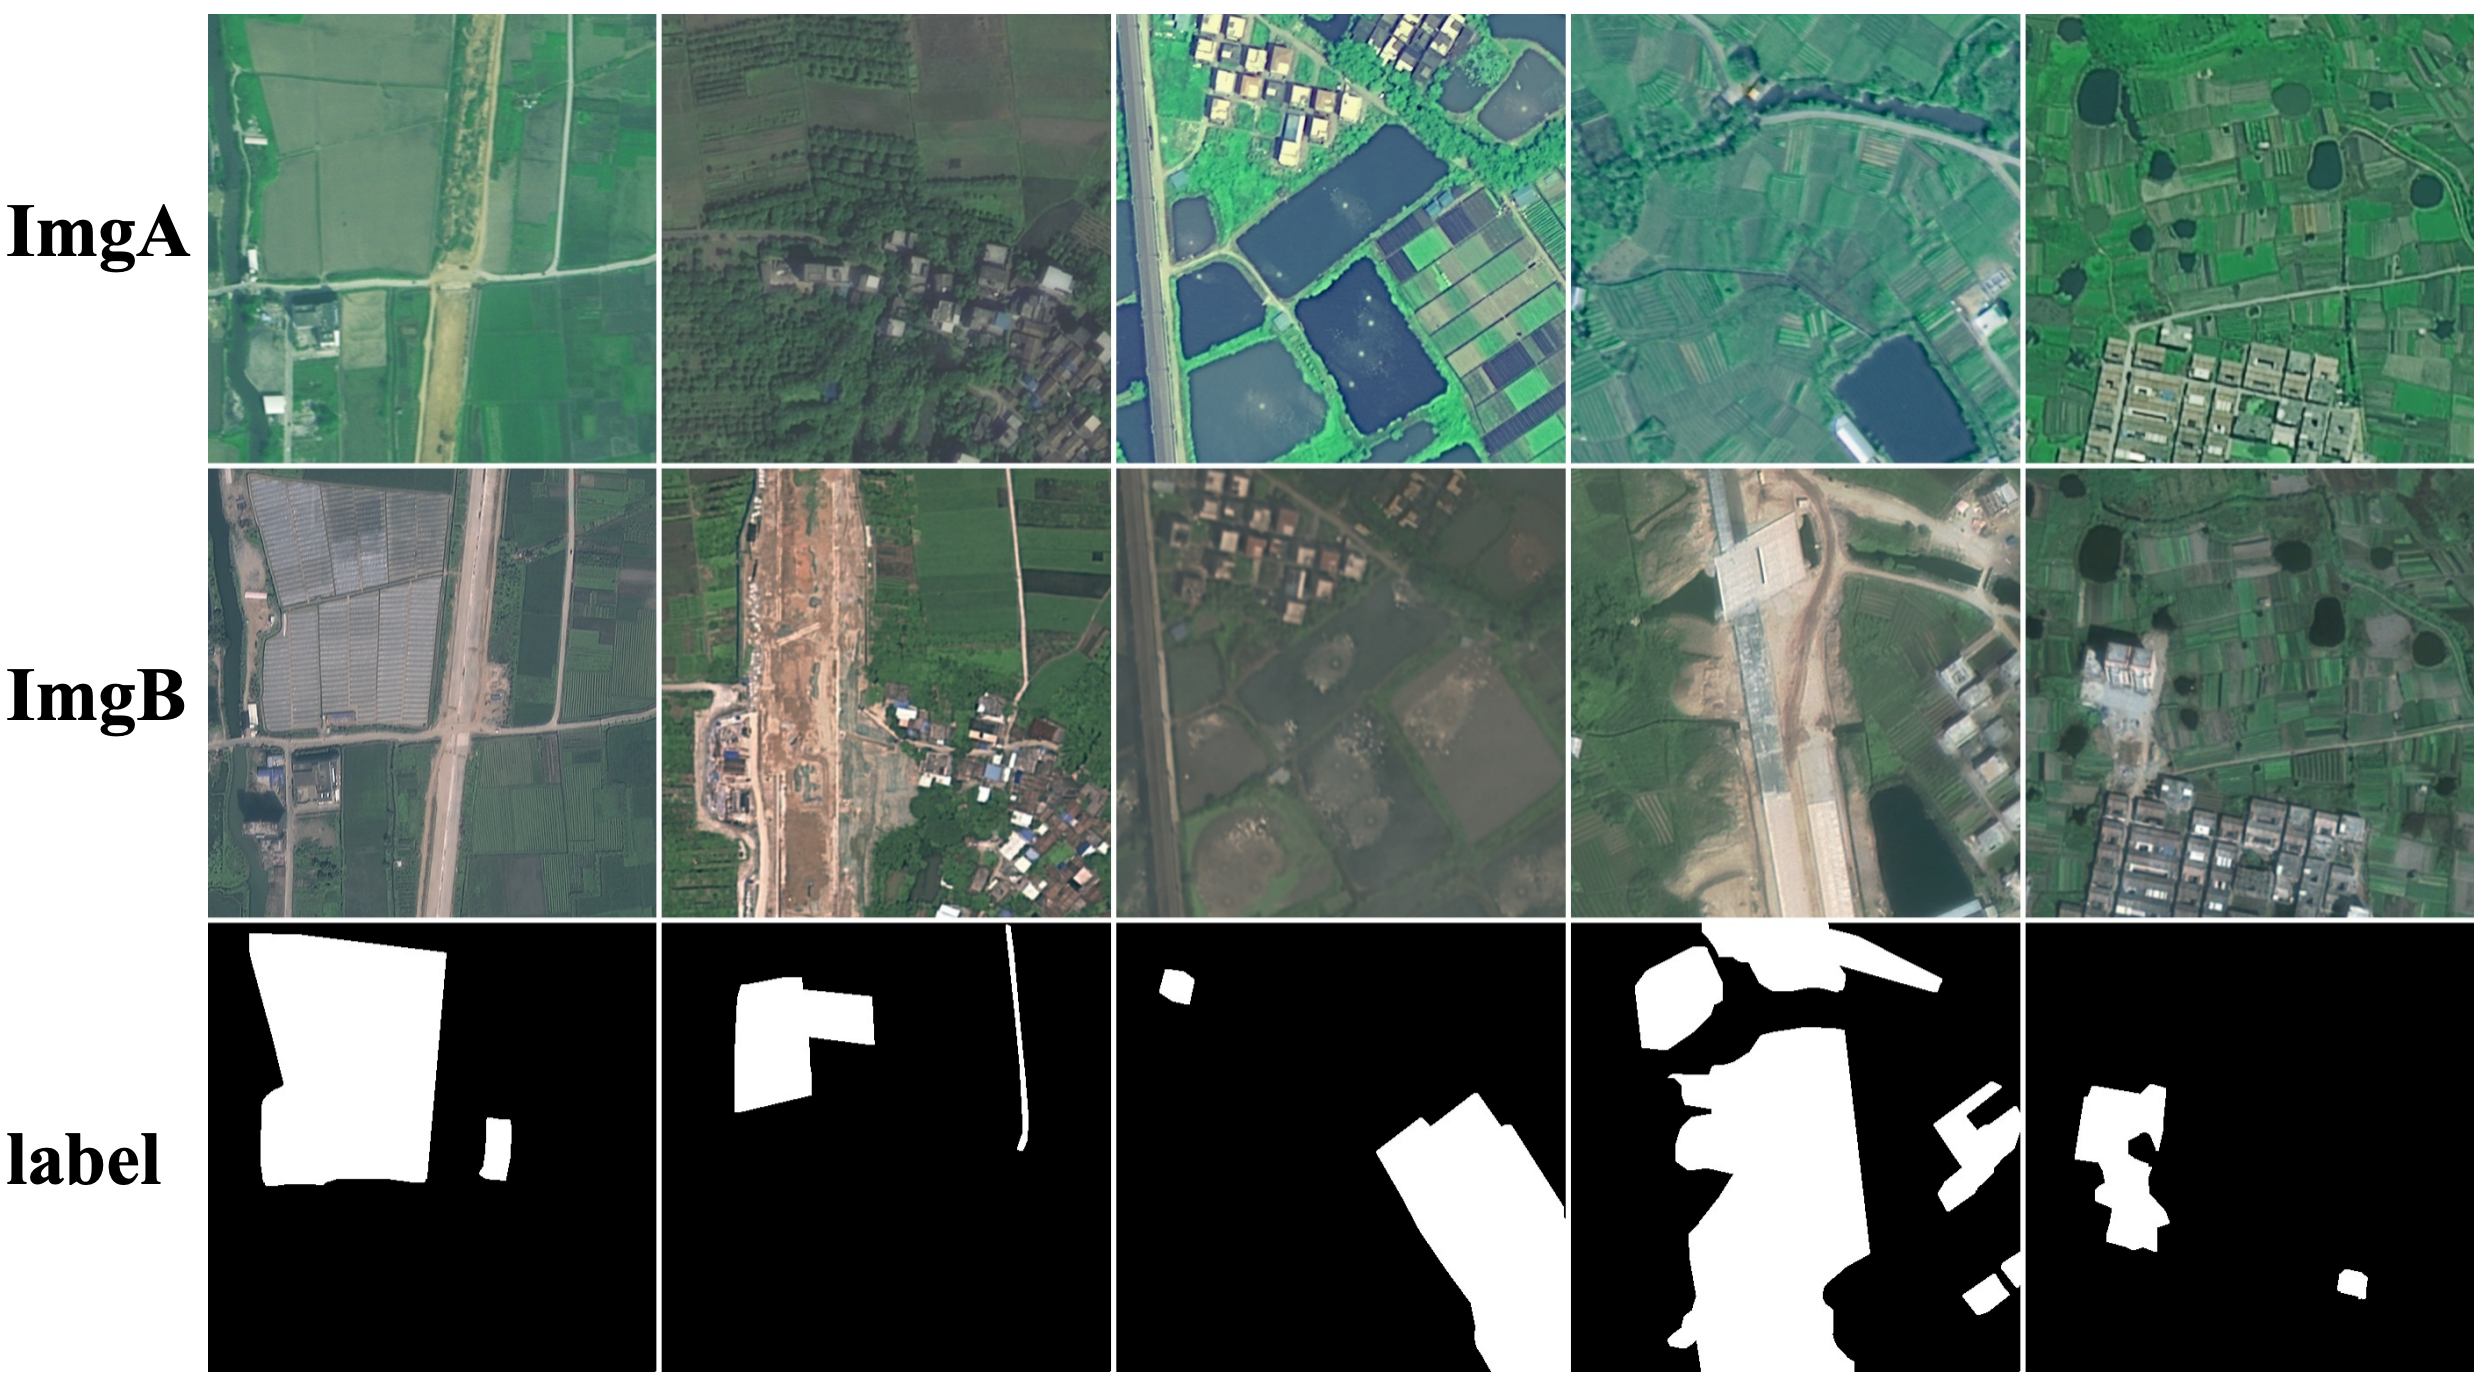
\includegraphics[width=0.75\textwidth]{paper_figures/变化检测任务与实验方法介绍/clcd.png}
  \caption{CLCD 数据集展示.}
  \label{fig:clcd}
\end{figure}

\subsubsection{PX-CLCD数据集}
Peixian耕地变化检测(PX-CLCD)数据集~\cite{miao_snunet3_2024}最初包含5170对具有1米空间分辨率、256×256像素的双时相图像。在数据集的构建过程中,按照6:2:2的比例将数据集划分为训练集、验证集和测试集。为了扩充数据集,研究人员通过应用随机翻转和旋转等数据增强技术,最终生成了PX-CLCD耕地变化检测数据集,分别代表2018年和2021年两年的耕地变化图像。如图~\ref{fig:pxclcd}所示,PX-CLCD数据集的变化类型主要包括耕地上新建温室、耕地上新修硬化道路、耕地上新建人工湖以及耕地上新建房屋等,这些变化类型在数据集中均得到了详细标注。

\begin{figure}[!htbp]
  \centering
  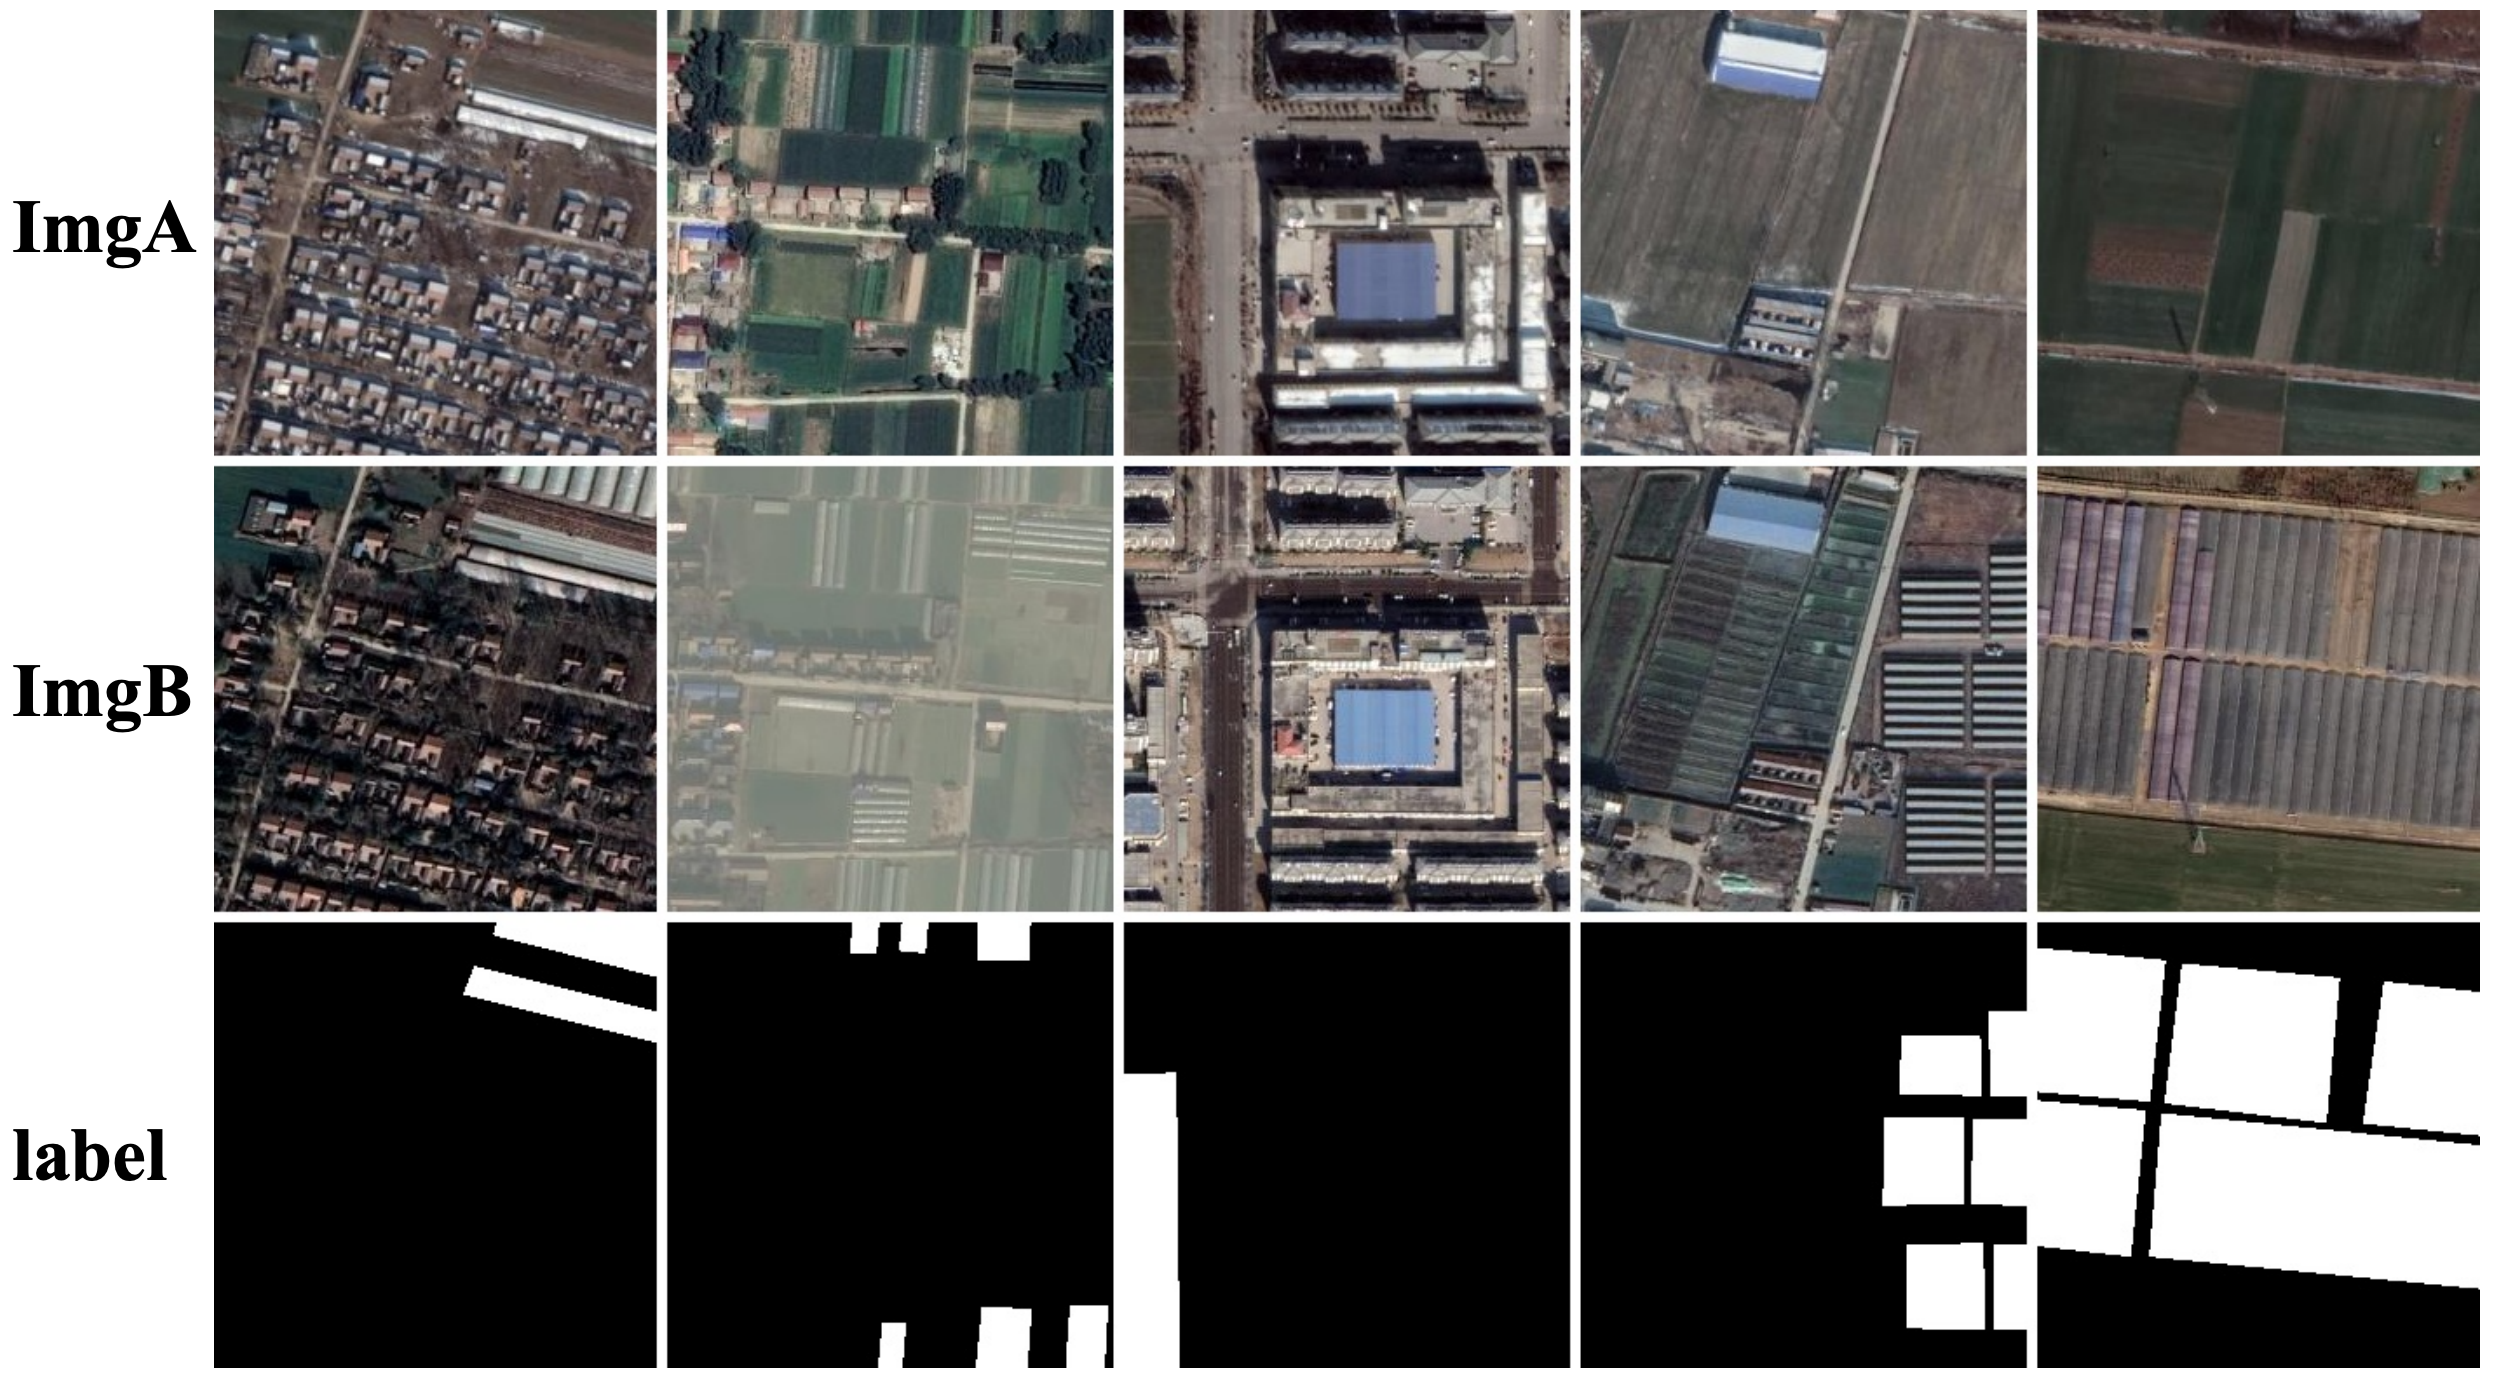
\includegraphics[width=0.75\textwidth]{paper_figures/变化检测任务与实验方法介绍/pxclcd.png}
  \caption{PX-CLCD 数据集展示.}
  \label{fig:pxclcd}
\end{figure}

\subsection{针对水体区域的变化检测数据集}
Water-CD 数据集~\cite{j_li_trsanet_2024}旨在促进水体变化检测,填补了变化检测任务在水体变化检测中的空白。如图~\ref{fig:watercd}所示,Water-CD 数据集包含来自中国长江流域的季节性湖泊,以及南亚朱姆纳河等地的各种季节性水体。Water-CD数据集卫星影像获取了空间分辨率为 10 m 的双时相遥感数据,包含红光(R)、绿光(G)和近红外(NIR)波段,影像均为 2016–2022 年间雨季和旱季拍摄的无云图像。Water-CD水体变化检测图像数据集包含 1149 对双时相影像,每对影像的尺寸为 512 × 512。

\begin{figure}[!htbp]
  \centering
  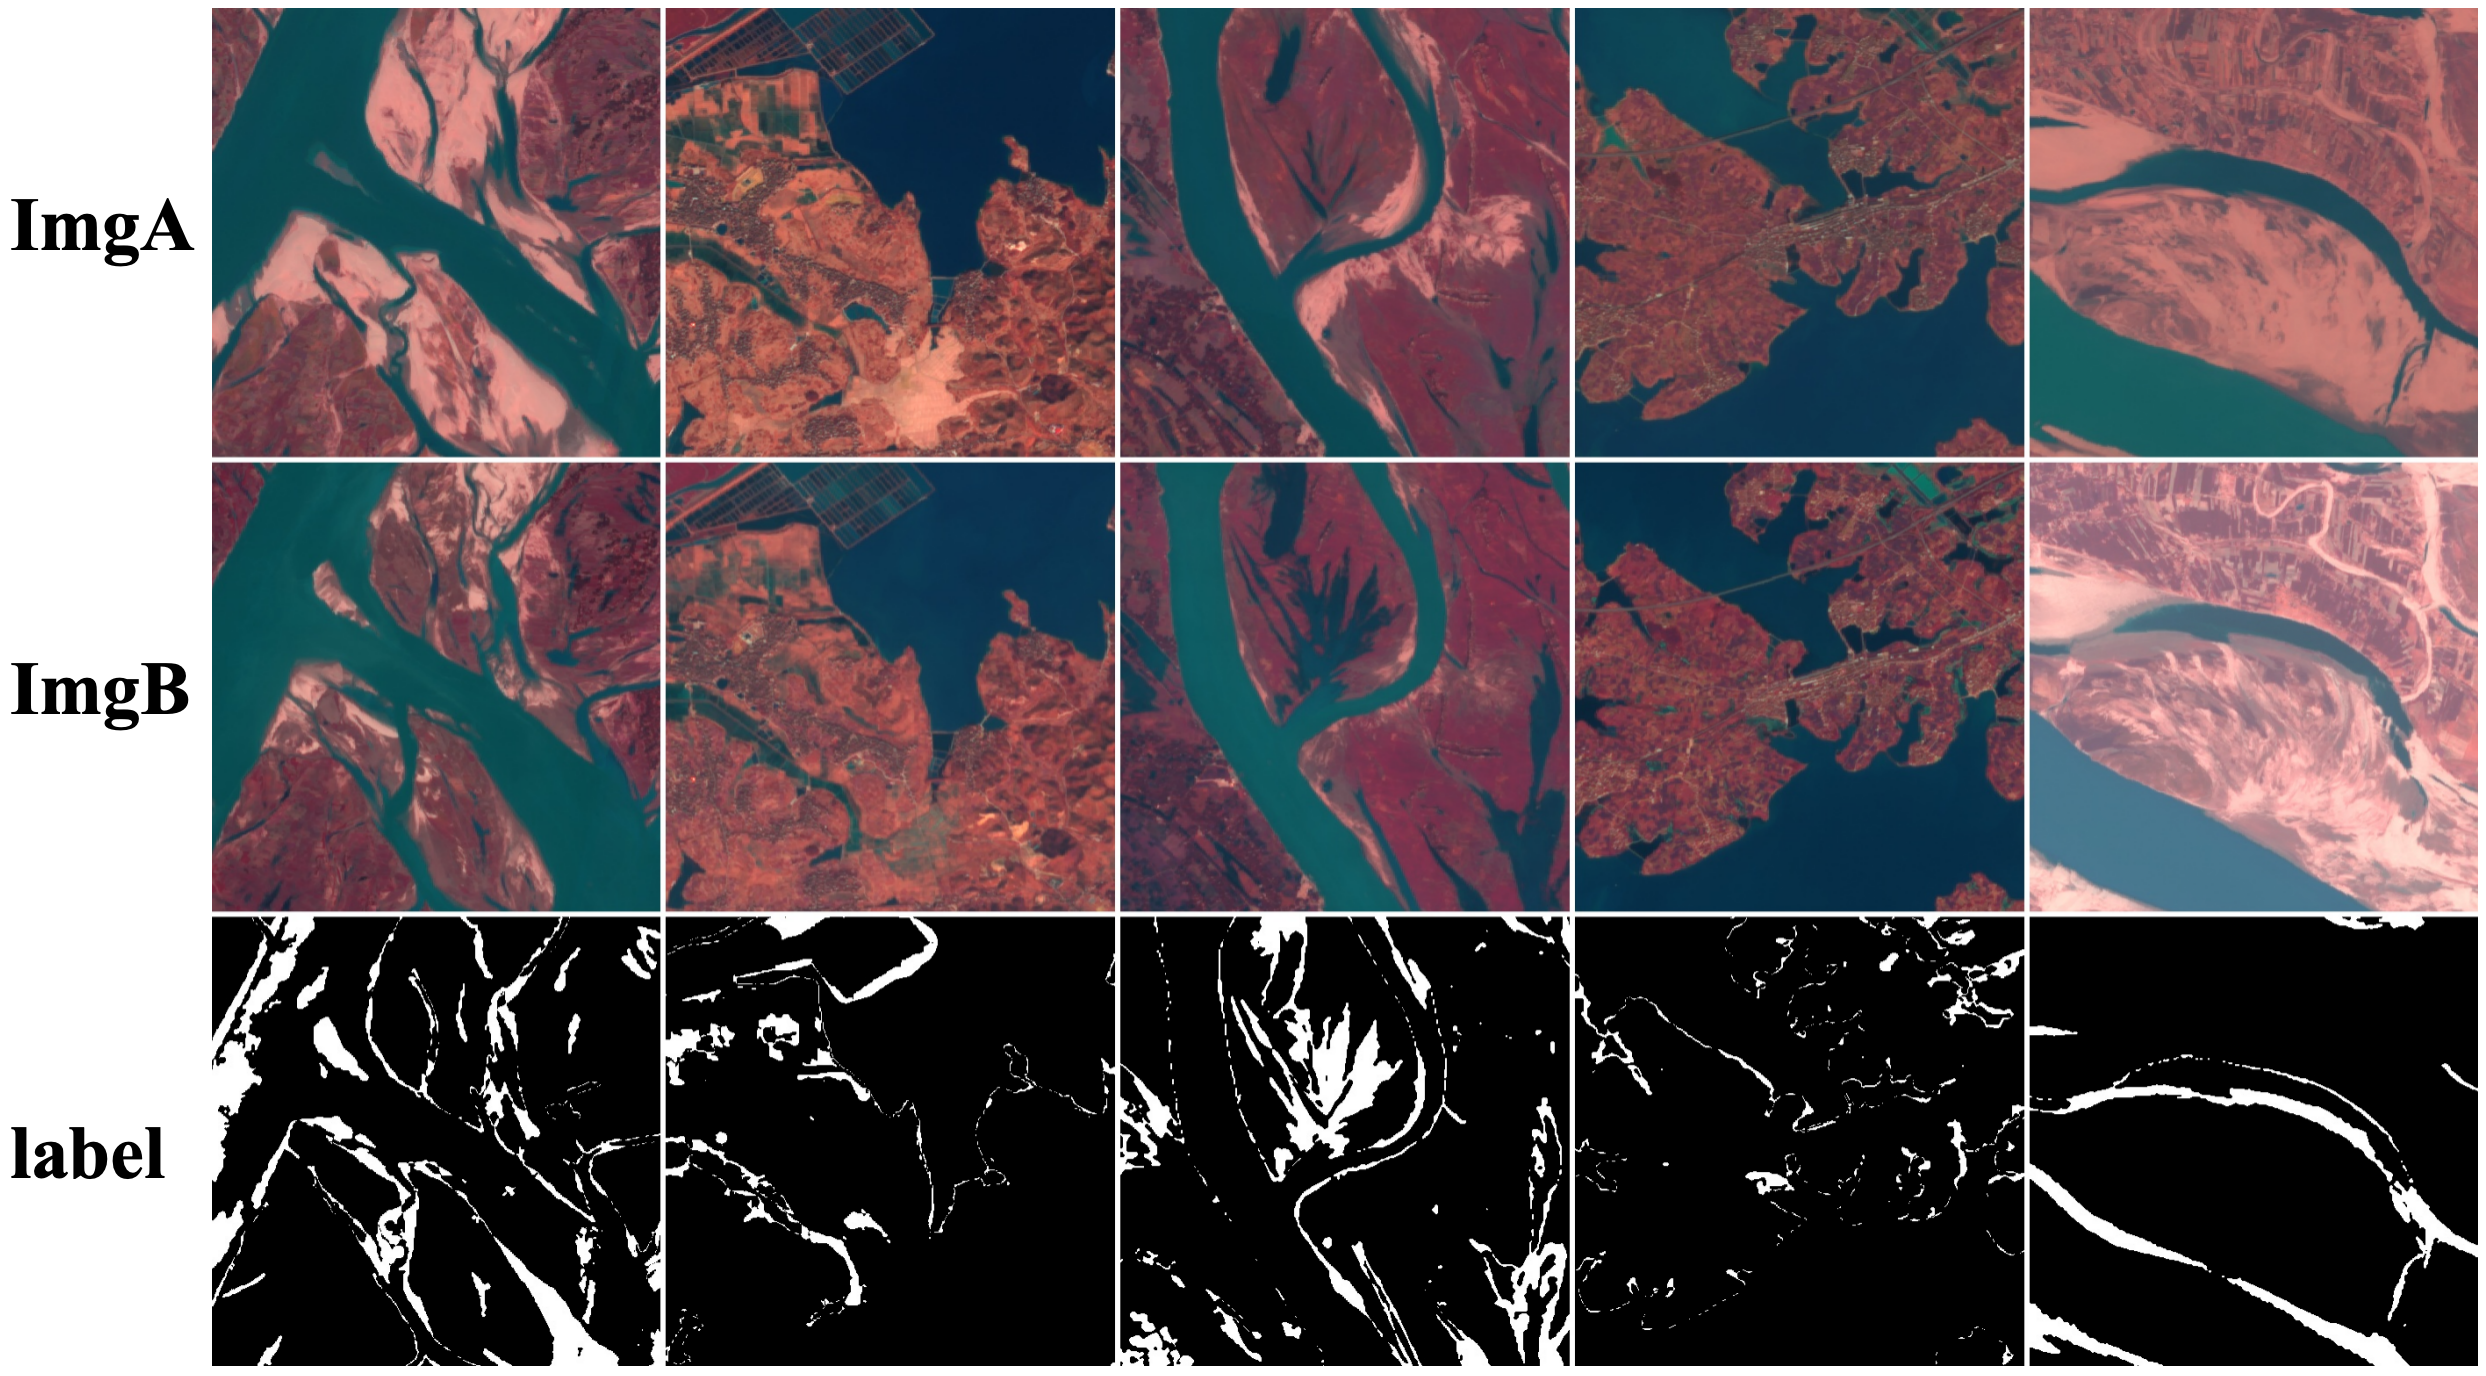
\includegraphics[width=0.75\textwidth]{paper_figures/变化检测任务与实验方法介绍/watercd.png}
  \caption{Water-CD 数据集展示.}
  \label{fig:watercd}
\end{figure}

\subsection{通用变化检测数据集}
\subsubsection{CDD数据集}
CDD变化检测数据集~\cite{Lebedev2018CHANGEDI}包含显示同一区域季节变化的卫星图像。该数据集通过收集来自Google Earth的数据创建,包括分辨率范围从0.03米到1米的图像。数据集中的图像被随机裁剪为256×256的大小。裁剪后,数据集被划分为训练集、验证集和测试集。训练集包含10000张图像,而验证集和测试集各包含3000张图像。该数据集旨在测试变化检测模型在同一区域随时间变化时识别变化的能力。如图~\ref{fig:cdd}所示,数据集包含多种变化类型,如城市发展、植被变化和水体变化,因此它是评估变化检测模型在不同场景下表现的有用工具。

\begin{figure}[!htbp]
  \centering
  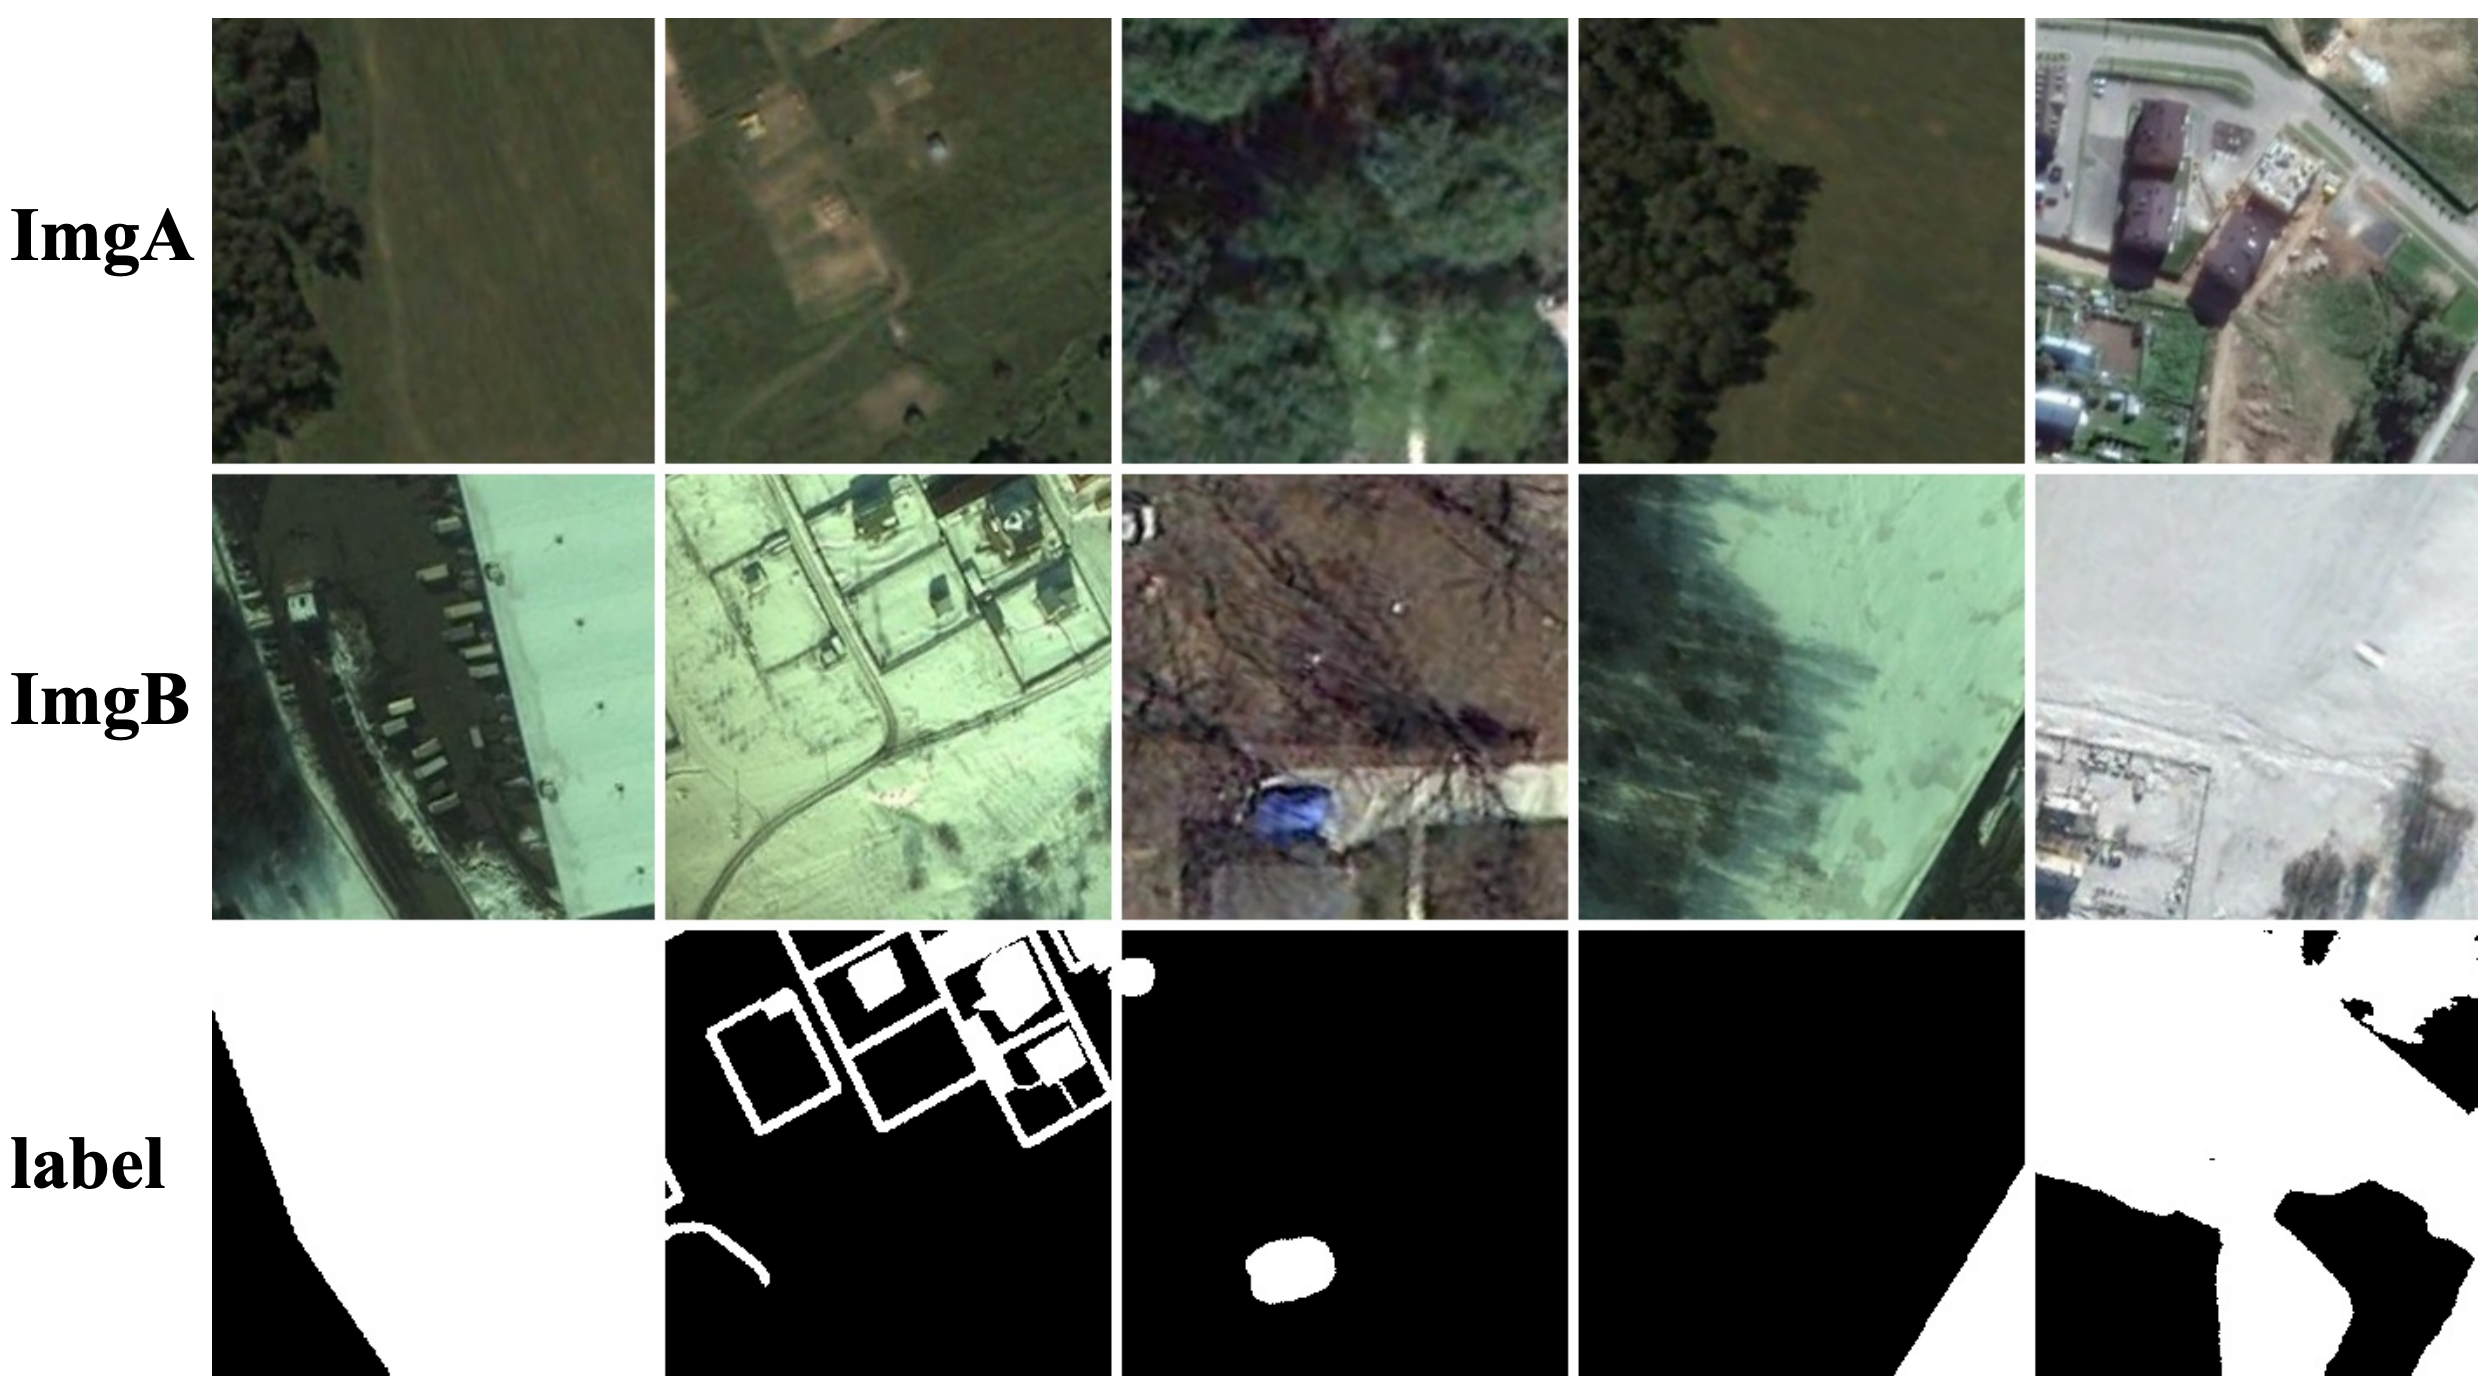
\includegraphics[width=0.75\textwidth]{paper_figures/变化检测任务与实验方法介绍/cdd.png}
  \caption{CDD 数据集展示.}
  \label{fig:cdd}
\end{figure}

\subsubsection{SYSU数据集}
SYSU-CD数据集~\cite{shi_deeply_2022}是一个包含20000对高分辨率航拍图像的集合,每张图像大小为256×256像素,图像采集自2007至2014年间的香港。该数据集包含多种变化类型,包括新建城市建筑、郊区扩展、建设前的地面准备、植被变化、道路扩展以及海上建筑等。如图~\ref{fig:sysu}所示,SYSU-CD数据集高度代表了城市变化,涵盖了大多数在城市环境中发生的变化类型。该数据集被划分为三部分:训练集、验证集和测试集,分别包含12000对、4000对和4000对图像。这种划分遵循了常用的实验程序。SYSU-CD数据集为评估和比较不同类型城市变化的变化检测算法性能提供了宝贵的资源。

\begin{figure}[!htbp]
  \centering
  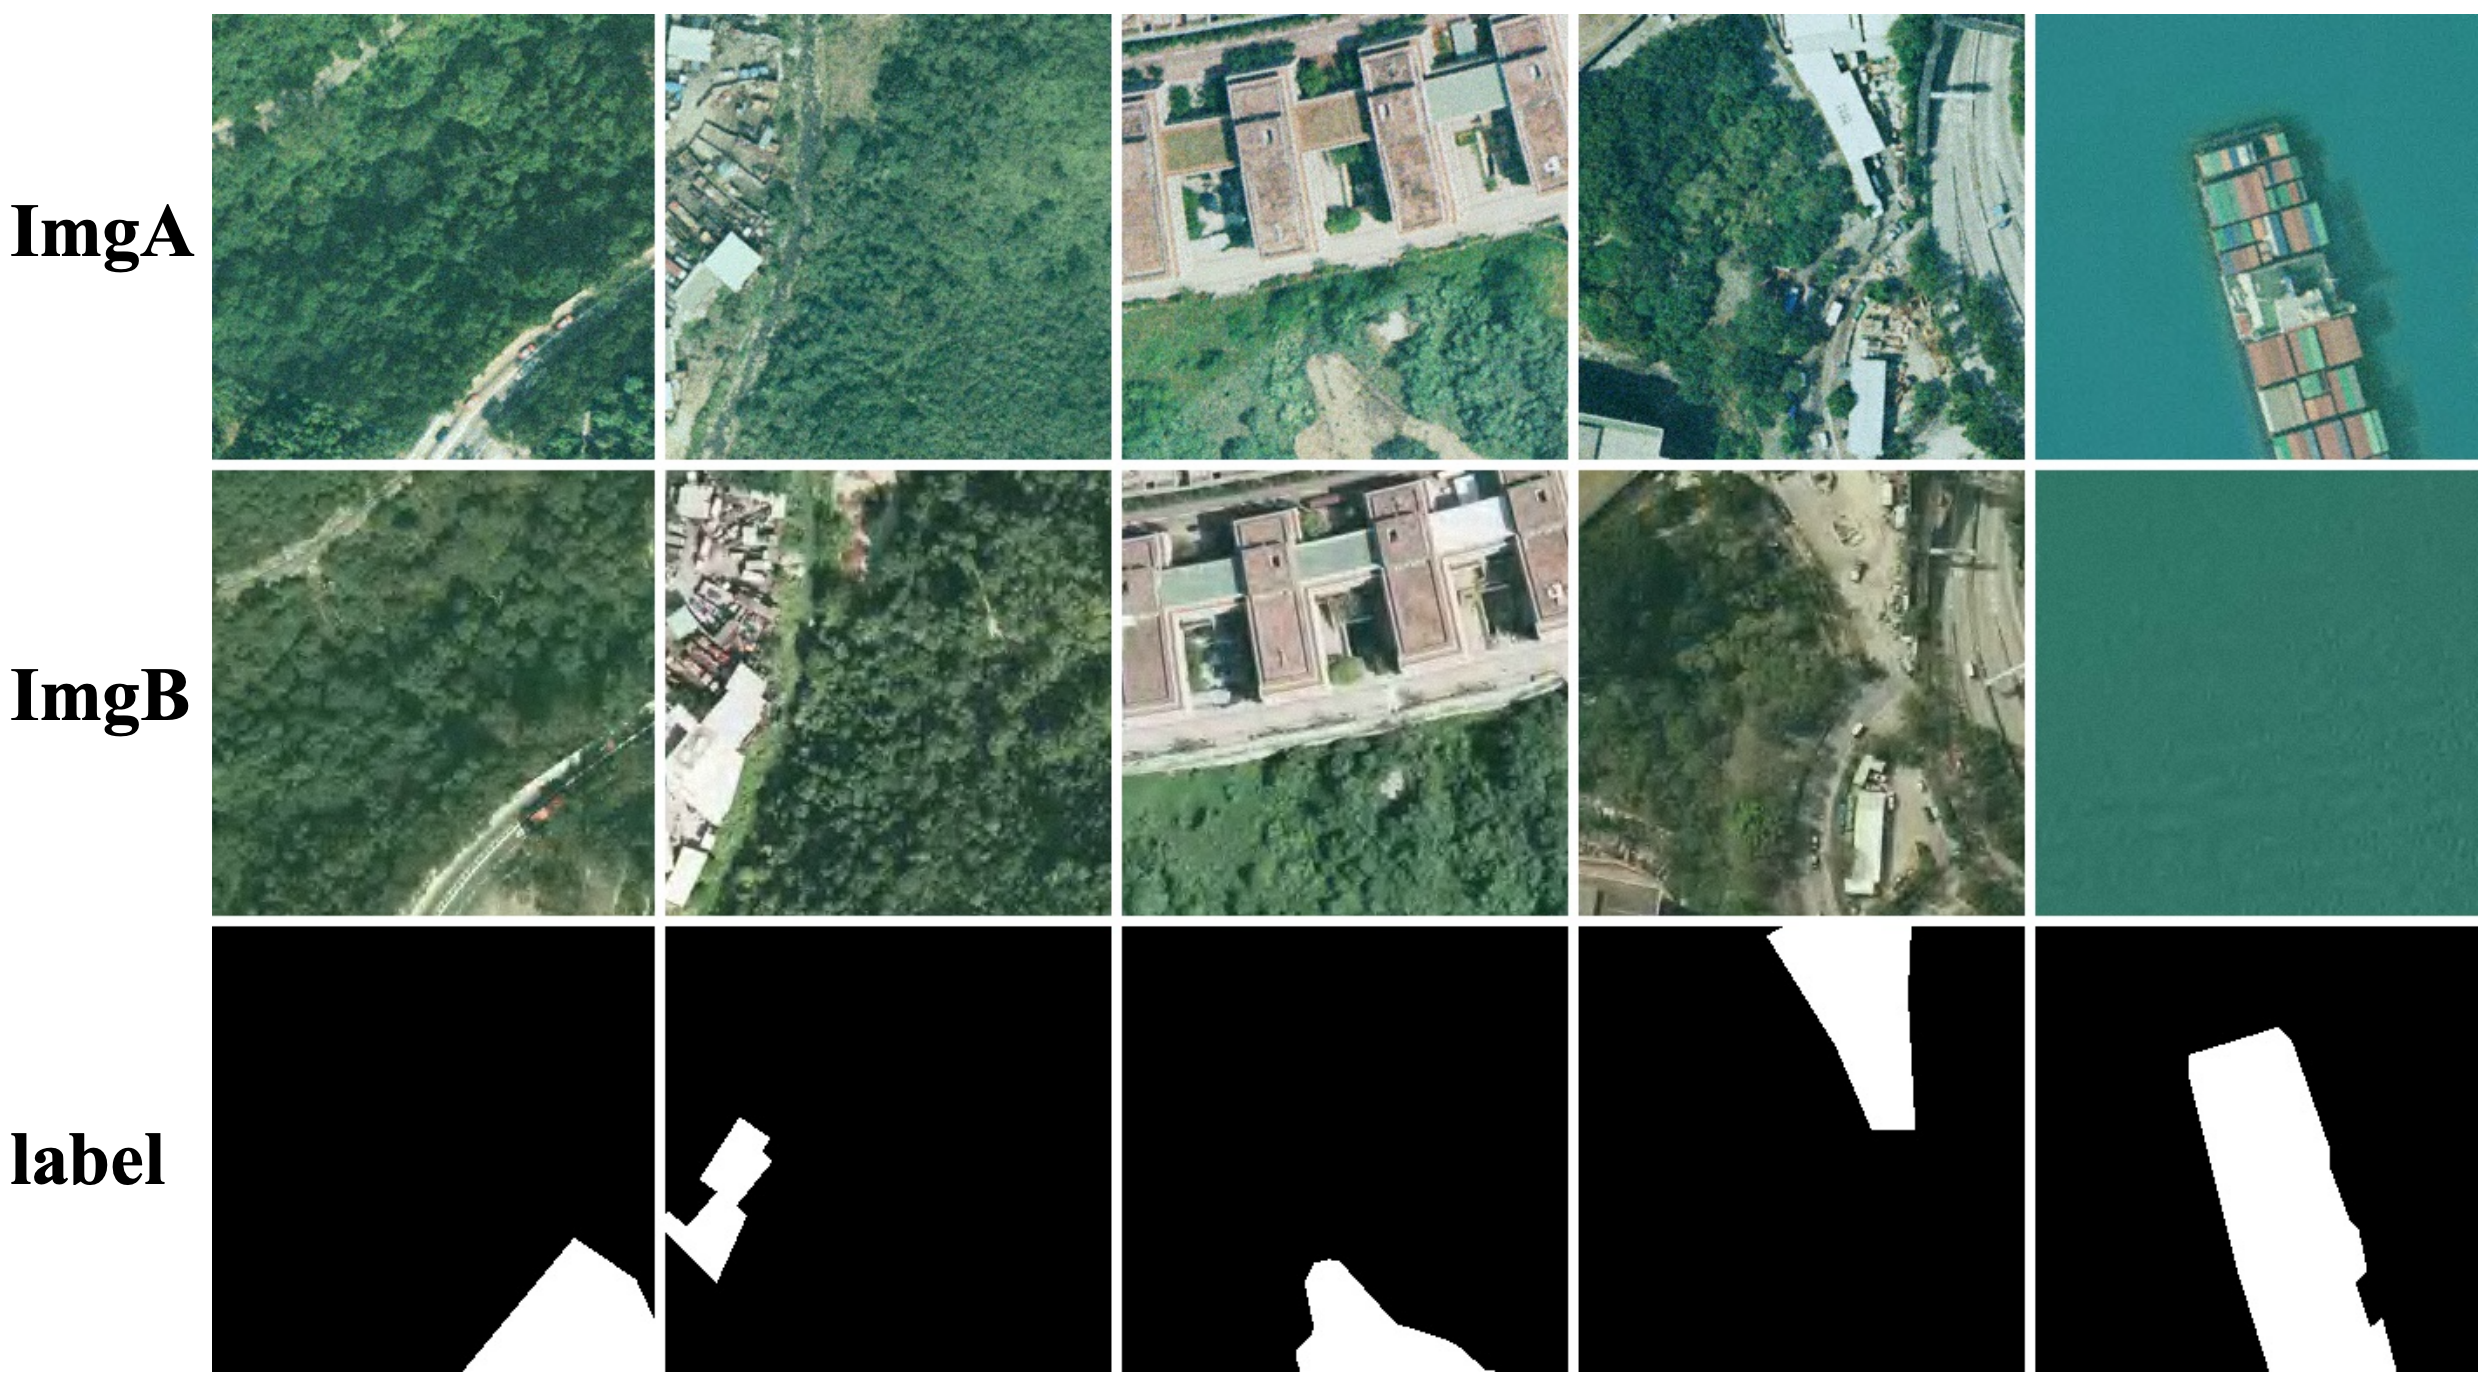
\includegraphics[width=0.75\textwidth]{paper_figures/变化检测任务与实验方法介绍/sysu.png}
  \caption{SYSU-CD 数据集展示.}
  \label{fig:sysu}
\end{figure}

\begin{figure}[!htbp]
  \centering
  \includegraphics[width=0.75\textwidth]{paper_figures/变化检测任务与实验方法介绍/msrscd.png}
  \caption{MSRSCD 数据集展示.}
  \label{fig:msrscd}
\end{figure}


\subsubsection{MSRSCD数据集}
MSRSCD数据集~\cite{Liu2025NetworkAD}在图像分辨率、变化类型、数据集大小和变化维度方面显著补充了现有的遥感影像变化检测数据集,进一步为变化检测任务提供了新的基准。该数据集包括2019年至2023年间在中国南方城市捕获的841对遥感图像,每张图像大小为1024×1024像素,空间分辨率为0.5米。数据集按照7:1:2的比例分为训练集、验证集和测试集。如图~\ref{fig:msrscd}所示,数据集中的主要变化类型包括新建筑、郊区扩张、植被变化和道路建设。

\begin{figure}[!htbp]
  \centering
  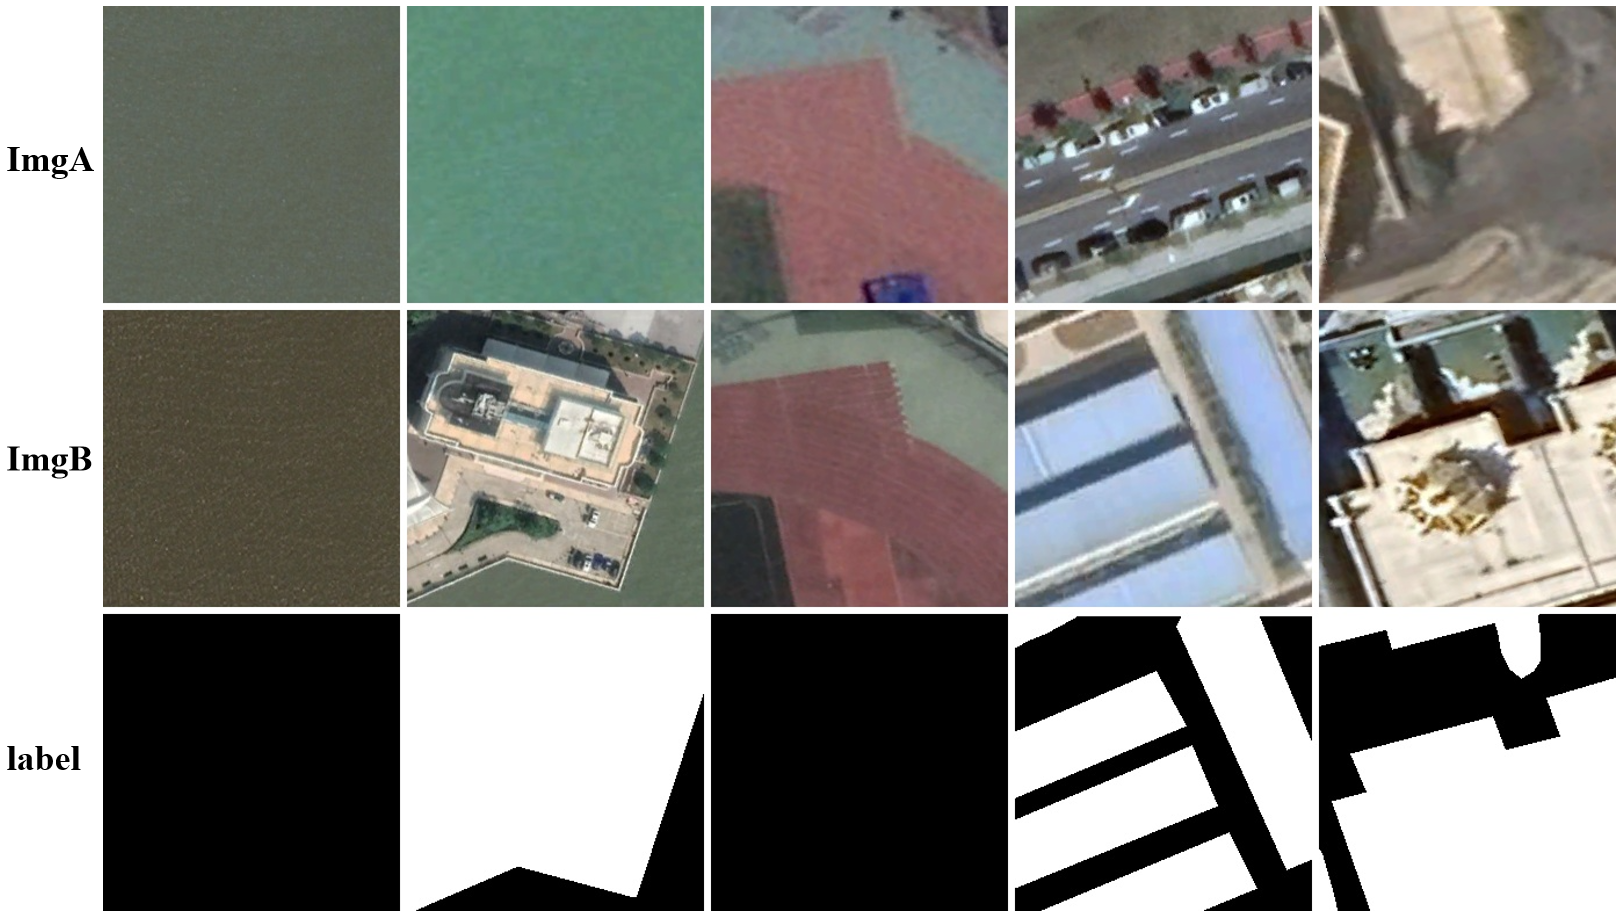
\includegraphics[width=0.75\textwidth]{paper_figures/变化检测任务与实验方法介绍/mlcd.png}
  \caption{MLCD 数据集展示.}
  \label{fig:mlcd}
\end{figure}

\subsubsection{MLCD数据集}
MLCD数据集~\cite{Huang2025SAMBasedEF}(Macao Land Change Detection)聚焦于澳门地区2008至2023年间的土地填海与植被动态变化,基于Google Earth Engine影像构建。如图~\ref{fig:mlcd}所示,该数据集包含10,000对已标注的$256\times256$遥感影像,空间分辨率为0.5–2米,为海岸地貌与土地利用演变研究提供了新的基准。


\begin{table}[!htbp]
\centering
\caption{本文所选用的遥感影像变化检测数据集概览}
\label{tab:change_detection_datasets_review}
\setlength{\tabcolsep}{4pt} % 列间距紧凑一些
\renewcommand{\arraystretch}{1.15}
\small
\begin{tabularx}{\textwidth}{@{} l c c c X X c @{}}
\toprule
\textbf{数据集} & \textbf{切片尺寸} & \textbf{数据总量} & \textbf{影像分辨率} & \textbf{影像地理位置} & \textbf{卫星} & \textbf{应用对象} \\
\midrule
LEVIR-CD~\cite{chen_spatial-temporal_2020}   & 1024$\times$1024 & 637    & 0.5 m        & American cities                                   & Google Earth                     & 建筑物 \\
LEVIR-CD+~\cite{chen_spatial-temporal_2020}  & 1024$\times$1024 & 985    & 0.5 m        & American cities                                   & Google Earth                     & 建筑物 \\
WHUCD~\cite{Ji2019FullyCN}     & 256$\times$256   & 7620   & 0.2 m        & Christchurch, New Zealand                          & --                                & 建筑物 \\
S2Looking~\cite{Shen2021S2LookingAS}  & 1024$\times$1024 & 5000   & 0.5--0.8 m   & --                                                & GaoFen / SuperView / BeiJing-2   & 建筑物 \\
MSRSCD~\cite{Liu2025NetworkAD}     & 1024$\times$1024 & 841    & 0.5 m        & Southern Chinese cities                           & --                                & 全场景 \\
SYSU-CD~\cite{shi_deeply_2022}    & 256$\times$256   & 20{,}000 & 0.5 m       & Hong Kong                                         & --                                & 全场景 \\
CDD~\cite{Lebedev2018CHANGEDI}        & 256$\times$256   & 16{,}000 & 0.03--0.1 m & --                                                & Google Earth                     & 全场景 \\
CLCD~\cite{Liu2022ACN}       & 512$\times$512   & 600    & 0.5--2 m     & Guangdong                                         & Gaofen-2                         & 耕地 \\
PX-CLCD~\cite{miao_snunet3_2024}    & 256$\times$256   & 5170   & 0.5--1 m     & Jiangsu                                           & Gaofen-2                         & 耕地 \\
Water-CD~\cite{j_li_trsanet_2024}   & 512$\times$512   & 1149   & 10 m         & Yangtze River; George Lake; Jamuna River          & Sentinel-2                       & 水体 \\
MLCD~\cite{Huang2025SAMBasedEF}       & 256$\times$256   & 10{,}000 & 0.5--2 m    & Macao                                             & Google Earth                     & 全场景 \\
\bottomrule
\end{tabularx}
\end{table}


如表~\ref{tab:change_detection_datasets_review}所示,总结了本文选取的当前主流变化检测数据集及其基本信息。这些数据集在多个维度上展现了高度的多样性,为全面评估算法性能提供了坚实基础。在应用对象上,既包括专注于建筑物变化的LEVIR-CD、WHU-CD与S2Looking数据集,也有面向耕地(CLCD、PX-CLCD)与水体(Water-CD)等特定自然资源监测的数据集,更有涵盖多种变化类型的全场景数据集(MSRSCD、SYSU-CD、CDD、MLCD)。在技术参数上,空间分辨率覆盖了从10米(Water-CD)的中等分辨率到亚米级乃至厘米级(如WHU-CD的0.2米和CDD的0.03米)的高分辨率影像;数据总量也从数百对样本的CLCD到两万对样本的SYSU-CD不等,充分考验了算法在不同数据规模下的性能。此外,这些数据集在地理范围与传感器类型上也极具代表性,地理上横跨了北美城市、新西兰、中国香港及内地多个省份,数据来源则涵盖了谷歌地球(Google Earth)、高分系列(Gaofen-2)、哨兵系列(Sentinel-2)等多种平台。这种多维度、多层次的多样性确保了本文的实验评估具有广泛的代表性,能够全面检验本文所提模型在不同场景、不同尺度和不同数据条件下的适应性与泛化能力。

\section{变化检测实验方法介绍}
\subsection{变化检测训练策略}
在遥感影像变化检测任务中,深度学习方法已经成为主流。为了使模型能够在不同类型和场景的变化检测任务中表现出色,合理的训练策略与数据增强方法至关重要。良好的训练策略不仅能够加速模型的收敛过程,还能提升模型的泛化能力;而数据增强则通过合成多样化的训练样本,提高模型在复杂场景下的鲁棒性,有效缓解过拟合问题。以下从训练集构建、模型设计、数据增强、损失函数以及优化策略等方面总结常用做法。

变化检测的训练策略通常包括训练集的构建、损失函数的设计以及优化策略的选择。为确保模型能够准确检测变化区域并实现有效分类,训练过程中的设计需要重点关注以下几个方面:
\begin{itemize}
 \item \textbf{训练集的构建}:在构建训练集时,应保证双时相影像来自同一地区,具有配准的地理坐标。此外,为了提高数据的多样性,可以通过裁剪大尺寸影像得到小块样本,从而提升模型的学习效率。
 
 \item \textbf{变化检测模型设计}:模型的设计通常采用孪生结构(Siamese Network)或编码-解码结构,以便有效提取和对比双时相影像特征。近年来,加入注意力机制、多尺度特征融合与特征交互模块的设计能够进一步提升模型对细粒度变化的感知能力。
 
 \item \textbf{数据增强策略}:常见的数据增强方法包括旋转、翻转、镜像以及色彩抖动等。这些操作可以增加样本多样性,使模型更好地适应不同光照、季节和传感器条件下的影像变化。
 
 \item \textbf{损失函数的设计}:损失函数通常采用交叉熵损失、Dice Loss 或两者的组合,以兼顾像素级分类精度与变化区域的整体一致性。在一些方法中,还会引入边界约束损失或对比损失,以增强模型对边界细节与类别差异的刻画能力。
 
 \item \textbf{优化策略的选择}:优化器一般选用Adam或AdamW,并结合余弦退火或多步学习率下降策略,以实现更稳定的收敛过程。同时,可采用早停(Early Stopping)机制,避免模型在后期出现过拟合。
\end{itemize}


\subsection{变化检测数据增强}
数据增强是深度学习中常用的技术,旨在通过人为生成新的训练样本,扩大训练集的多样性,从而提高模型的鲁棒性和泛化能力。在遥感影像变化检测任务中,数据增强的主要目标是模拟各种可能的变化场景,帮助模型在面对不同的环境条件时仍然能保持良好的性能。常见的变化检测数据增强方法包括:

\textbf{几何变换}:几何变换通过对图像进行旋转、缩放、翻转和裁剪等操作,模拟不同视角和尺度下的变化。通过这种方式,模型能够学习到变化区域在不同视角和不同分辨率下的表现,从而提升模型对这些变化的识别能力。尤其是在多时相影像变化检测任务中,图像的旋转和裁剪能够有效地模拟不同时间点拍摄的影像之间的几何差异。

\textbf{光照变化}:由于遥感影像的拍摄时间、季节以及天气条件的不同,光照变化对图像的影响是不可忽视的。通过对图像的亮度、对比度和饱和度进行调整,数据增强方法可以模拟不同光照条件下的影像变化。这有助于模型学习到变化区域在不同光照下的表现,增加其在不同环境条件下的鲁棒性。

\textbf{噪声添加}:遥感影像中经常存在各种噪声,包括盐噪声、椒噪声和高斯噪声等。通过在图像中加入不同类型的噪声,数据增强可以模拟传感器噪声和环境干扰。这有助于提高模型在实际应用中对噪声的处理能力,使其在高噪声环境下仍然能够准确检测到变化区域。

\textbf{图像变换和混合}:图像变换技术,如图像融合、样式转换(style transfer)和伪标签生成等方法,能够进一步丰富训练样本的多样性。例如,利用生成对抗网络(GAN)生成样式相似但内容不同的影像,可以为模型提供更多样化的变化场景。另外,图像混合方法(如Mixup)也可以通过将两幅图像的像素值加权混合,合成出新的训练样本,进一步提高模型对变化区域的感知能力。

\textbf{随机裁剪与填充}:随机裁剪可以帮助模型聚焦于局部区域的变化,这对于提高模型在变化细节处理上的能力至关重要。此外,在进行裁剪时,通常还会在裁剪后的图像中进行填充操作,确保输入图像的尺寸一致,这有助于网络保持输入图像的尺寸一致性。



\begin{sidewaystable}[htbp]
\centering
\scriptsize
\caption{不同研究侧重的变化检测模型汇总}
\label{tab:cd_models_summary}
\begin{tabularx}{\textheight}{@{}l X@{}} % 注意这里要用 \textheight 替代 \textwidth
\toprule
\textbf{研究侧重} & \textbf{模型汇总} \\
\midrule
结合CNN & CDNet~\cite{Alcantarilla2016StreetviewCD}、FC-Siam-Di~\cite{Daudt2018FullyCS}、FresUNet~\cite{Daudt2018MultitaskLF}、L-UNet~\cite{Papadomanolaki2021ADM}、DTCDSCN~\cite{Liu2019BuildingCD}、P2V~\cite{lin_transition_2023}、JFSDNet~\cite{Zhou2022JointFD}、LGPNet~\cite{Liu2022BuildingCD}、AFCF3D-Net~\cite{Ye2023AdjacentLevelFC}、STFF-GA~\cite{h_wei_spatio-temporal_2024}、AMFNet~\cite{zhan_amfnet_2024}、TRSANet~\cite{j_li_trsanet_2024}、HANet~\cite{Han2024HANetAH}、AFCF3DNet~\cite{ye_adjacent-level_2023}、AGFormer~\cite{Chen2025AGFormerAA}、SGSLN~\cite{zhao_exchanging_2023}、FCCDN~\cite{Chen2021FCCDNFC}、AANet~\cite{Hang2024AANetAA}、EfficientCD~\cite{dong_efficientcd_2024}、SSCD~\cite{Wang2024SummatorSubtractorNM}、MSCANet~\cite{m_liu_cnn-transformer_2022}\\
\midrule
结合注意力机制 & STANet~\cite{chen_spatial-temporal_2020}、HMCNet~\cite{Wang2022HMCNetHE}、DMATNet~\cite{Song2022RemoteSI}、DSAMNet~\cite{shi_deeply_2022}、IRA-MRSNet~\cite{Ling2022IRAMRSNetAN}、ISDANet~\cite{h_ren_interactive_2025}、HATNet~\cite{Xu2024HybridAT}、CDNeXt~\cite{wei_robust_2024}、DMINet~\cite{feng_change_2023}、BASNet~\cite{z_wang_bitemporal_2024}、AMTNet~\cite{Liu2023AnAM}、ACABFNet~\cite{Song2023AxialCA}、ACAHNet~\cite{Zhang2023AsymmetricCH}\\
\midrule
结合Transformer & BIT~\cite{chen_remote_2022}、MFATNet~\cite{Mao2022MFATNetMF}、ChangeFormer~\cite{bandara2022transformer}、HMCNet~\cite{Wang2022HMCNetHE}、TransUNetCD~\cite{Li2022TransUNetCDAH}、STransUNet~\cite{Yuan2022STransUNetAS}、SwinSUNet~\cite{zhang_swinsunet_2022}、RCDT~\cite{Lu2022RCDTRR}、DgFA~\cite{f_zhou_dual-granularity_2025}、FTransDF-Net~\cite{li_dual_2025}、ScratchFormer~\cite{Noman2023RemoteSC}、Conv-former~\cite{Yang2025ConvFormerCDHC}、EATDer~\cite{Ma2024EATDerEA}\\
\midrule
结合Mamba & CDMamba~\cite{zhang_cdmamba_2025}、RSM-CD~\cite{zhao_rs-mamba_2024}、CWmamba~\cite{Liu2025CWmambaLC}、CD-STMamba~\cite{Liu2025CDSTMambaTR}、HFIFNet~\cite{Han2025HFIFNetHF}、LCCDMamba~\cite{Huang2025LCCDMambaVS}、Hybrid-MambaCD~\cite{Feng2025HybridMambaCDHM}、ConMamba~\cite{Dong2024ConMambaCA}、FEMCD~\cite{Xing2025FrequencyEnhancedMF}、IMDCD~\cite{Liu2024IterativeMD}、MSA~\cite{Huang2025MSAMS}\\
\midrule
AI 基础模型 & SGANet~\cite{j_chen_sganet_2025}、SAM-Mamba~\cite{Li2025SAMMambaATC}、DepthCD~\cite{Zhou2025DepthCDDP}、EFI-SAM~\cite{Huang2025SAMBasedEF}、SAM-CD2~\cite{Sun2024SegmentAM}、DED-SAM~\cite{Qiu2025DEDSAMAdaptingSA}\\
\midrule
双时相特征融合 & SNUNet~\cite{Fang2021SNUNetCDAD}、DSIFN~\cite{Zhang2020ADS}、ICIF-Net~\cite{Feng2022ICIFNetIC}、DPCCNet~\cite{Papadomanolaki2021ADM}、DARNet~\cite{li_densely_2022}、ISNet~\cite{Cheng2022ISNetTI}、MFCF-Net~\cite{b_huang_remote-sensing_2024}、CMCD~\cite{li_cmcd_2025}、MIFNet~\cite{w_xie_mifnet_2025}、GASNet~\cite{zhang_global-aware_2023}、FHD~\cite{pei_feature_2022}、D-TNet~\cite{wan_d-tnet_2022-3}、SSANet~\cite{Jiang2022JointVL}、SFFCE-CD~\cite{y_xing_sffce-cd_2025}、FTA-Net~\cite{t_zhu_fta-net_2025}、HASNet~\cite{c_tao_hasnet_2025}、DDAM-Net~\cite{feng_ddam-net_2024}、SNUNet3+~\cite{miao_snunet3_2024}、CGNet~\cite{han_change_2023}、ELGCNet~\cite{m_noman_elgc-net_2024}、DEDANet~\cite{Li2025DifferenceEA}、DMFANet~\cite{Zhan2025DifferenceAwareMF}、SAFDNet~\cite{Fu2025BeyondCD}、AEGL-Net~\cite{Ying2025AEGLNetAM}、MSNet~\cite{Liu2025NetworkAD}、DFFNet~\cite{Liu2025FullScaleCD}、DSCRNet ~\cite{Zhang2025ADS}、B2CNet~\cite{Zhang2024B2CNetAP}、Changer~\cite{Fang2022ChangerFI}、MIN-Net~\cite{Zhou2024MultistageIN}、CACG-Net~\cite{Liu2024CandidateAwareAC}、PCAANet~\cite{Xu2023ProgressiveCA}、HCGMNet~\cite{Han2023HCGMNetAH}、STRobustNet~\cite{Zhang2025STRobustNetEC}\\
\midrule
新型架构 & STDF-CD~\cite{y_zhou_stdf_2025}、UA-BCD~\cite{li_overcoming_2025}、RSBuilding~\cite{wang_rsbuilding_2024}、MLDFNet~\cite{d_sidekejiang_mldfnet_2025}、DSFI-CD~\cite{x_li_dsfi-cd_2025}\\
\bottomrule
\end{tabularx}
\end{sidewaystable}

\subsection{变化检测性能评估方法}
为了验证本文提出的方法的有效性,本文与多种先进的变化检测方法进行了详细的对比。通过与先进变化检测模型在相同数据集上的性能比较,能够全面评估所提出方法的优势和创新点。对于每个数据集,计算了多个常用的评估指标,如交并比(IoU)、F1、精度(OA)、召回率(Rec)、精确率(Prec)。这些指标能够综合反映算法在不同类型变化区域上的检测能力和准确性。由于本文所针对的是通用变化检测模型,即分辨样本中发生变化的区域。通常这种样本是类别不均衡样本,因此,在本文中,选用前景类(变化区域)的 IoU 作为评价算法性能的核心标准。这是因为在变化检测任务中,未变化像素(背景)的数量通常远超变化像素(前景),存在严重的类别不平衡问题。在此情况下,像总体准确度(OA)这样的指标会被背景类主导,无法真实反映模型对关键变化区域的识别能力,而IoU能够更鲁棒、更公平地衡量模型在前景类别上的表现。如下所示,定义了各个评估指标的计算公式:
\begin{equation}
OA = \frac{TP + TN}{TP + TN + FN + FP}
\end{equation}

\begin{equation}
IoU = \frac{TP}{TP + FN + FP}
\end{equation}

\begin{equation}
Rec = \frac{TP}{TP + FN}
\end{equation}

\begin{equation}
Prec = \frac{TP}{TP + FP}
\end{equation}

\begin{equation}
F1 = \frac{2 \cdot Prec \cdot Rec}{Prec + Rec}
\end{equation}
其中,TP表示真正例的数量,TN表示真反例的数量,FP表示假阳例的数量,FN表示假反例的数量。这些指标提供了一个综合评估算法在遥感影像中检测和分类变化的能力。

\subsection{本文实验细节}

本文设计的算法的代码框架均在PyTorch编程环境下构建的,基于mmsegmentation库开发了一套变化检测任务训练框架(MMRSCD)。同时,由于基于mmsegmentation 架构的变化检测代码开发存在代码架构封装太完整,因此不适合变化检测模型的开发。因此,基于 Pytorch-Lightning 框架设计了新的变化检测实验平台remote-sensing-change-detection 项目,更适合结合现今的 AI 基础模型开发变化检测算法。MMRSCD与remote-sensing-change-detection框架部署在Ubuntu系统上,实验选取的训练 GPU 包括 NVIDIA 3090、NVIDIA 4090、NVIDIA V100 以及 NVIDIA A100,以促进加速模型训练。为了深入分析本文提出模型的内在性能,本文有意限制了数据增强技术,仅使用了常用的几何变换数据增强,从而最小化外部因素对模型性能的影响。在模型优化方面,本文使用了AdamW优化器,学习率通常设置为0.0001或 0.0003,同时设置了WarmUP 训练策略。在训练过程中,本文所设计的所有模型的损失函数为二分类交叉熵损失。在实验阶段,持续监控验证集上的变化区域IoU指标,标记出表现最好的模型用于后续的最终评估。

在 ChangeCLIP 模型中,为了生成与遥感图像对应的文本提示,初步推理是通过 CLIP 模型对从数据集中提取的原始图像切片进行的。56 个预定义类别的推理结果被系统地存储在数据库中。在训练阶段,我们动态地从该数据库中检索出 9 个高置信度类别,以组装前景和背景特征的文本提示。因此,这种方法最终形成了一个设计良好的多模态输入策略,涵盖了视觉和文本数据。因此,基于 ChangeCLIP 模型引入这种多模态数据构建并没有妥协整体训练效率。

同时,在本文的实验中,除 ChangeCLIP 需要对大尺寸图片进行提前的 $256\times 256$ 的裁剪,以便使用 CLIP 模型对切片生成预置的推理类别结果外,其他模型在训练过程中,若原始数据集尺寸大于 $256\times 256$,则均采用随机裁剪的方式进行训练,裁剪尺寸为 $256\times 256$。在推理过程中,对大尺寸影像采用滑窗预测的方式进行推理得到推理结果。为确保实验的公平性,在全文的实验中,推理过程未采用 TTA 等推理策略进行优化。

\subsection{本文实验对比模型汇总分析}

表~\ref{tab:cd_models_summary} 汇总了近年来遥感影像变化检测领域中,不同研究侧重的变化检测模型。根据模型的架构和设计理念,这些模型可以大致分为如下几类。首先,以卷积神经网络(CNN)为基础的经典变化检测方法奠定了深度学习变化检测的基石。为了增强CNN的特征表达能力,许多研究在其上引入了注意力机制,使其能自适应地聚焦于关键变化区域。随着技术发展,以Transformer架构为代表的模型,利用其自注意力机制的全局建模优势,有效克服了CNN感受野受限的问题,成为近年来的研究主流。同时,也涌现了大量结合两者优点的CNN与Transformer混合架构。近年来不断涌现的前沿架构,包括以线性复杂度实现长距离依赖建模的Mamba架构,以及利用大规模预训练知识、展现出强大泛化能力的AI基础模型,为变化检测带来了新的性能突破。除此之外,不论采用何种骨干网络,如何强化双时相特征的融合与差异表达始终是变化检测的核心问题。该表中此类模型数量最多,涵盖了从特征交互、差异增强到边界感知等多种技术路径。此外,还有部分新型架构,它们基于扩散模型、海量样本以及特定情景而构建变化检测模型。从上述的分析可以看出,本文的对比实验涵盖了当前变化检测领域的主流方法,确保了实验结果的全面性和代表性。

\section{本章小结}

本章系统地介绍了遥感影像变化检测(RSCD)的任务背景、关键技术环节、常用的实验数据集以及标准的实验方法,为后续章节的算法研究与验证奠定了坚实的基础。首先,本章明确了变化检测任务的核心目标,即识别并定位双时相遥感影像间的地表变化。内容涵盖了从双时相影像配准、差异特征分析到变化区域识别与分类等一系列关键步骤,并强调了随着深度学习技术的发展,变化检测方法已从传统的像素级对比演进为基于深度神经网络的自动化特征学习,显著提升了检测的精度与鲁棒性。其次,为了全面验证后续章节所提算法的有效性和泛化能力,本章详细梳理并介绍了多个具有代表性的公开变化检测数据集。这些数据集按变化类型可分为建筑物变化(LEVIR-CD/CD+、S2Looking、WHUCD)、农田变化(CLCD、PX-CLCD)、水体变化(Water-CD)以及通用场景变化(CDD、SYSU-CD、MSRSC、MLCD),覆盖了多样的地理环境、分辨率和变化模式。最后,本章概述了变化检测的标准化实验流程,包括训练策略(如损失函数选择、优化器策略以及WarmUP训练策略)和数据增强方法。这些方法旨在提升模型的收敛速度、鲁棒性与泛化能力。总而言之,本章所介绍的理论基础、基准数据集和实验方法共同构成了一个系统性的变化检测实验体系,将为后续第三至第六章中本文所提出的创新模型的性能验证,提供统一、公平的实验基准。

% 
\chapter{变化检测任务基础范式设计}

\section{引言}
遥感影像变化检测旨在通过比较不同时间获取的同一地理区域影像,自动识别地表变化区域。该任务在土地利用监测、城市扩张分析、生态保护和灾害评估等应用中具有重要意义~\cite{ting_bai_deep_2023}。在计算机视觉领域,变化检测和图像分割均被视为像素级预测任务~\cite{YGXB202309001}。几乎所有像素级任务的算法都采用编码器–解码器架构,其中编码器将输入数据转化为高维特征,解码器则将这些特征重构为特定任务所需的形式。然而,变化检测任务的独特之处在于其对双时相影像的处理,通常需要使用Siamese编码器设计~\cite{dong_efficientcd_2024}。因此,目前大多数变化检测算法均基于深度学习架构~\cite{chen_remote_2022, zhang_swinsunet_2022, wang2022unetformer}。

% % (可选)在导言区统一设置最大高度
% \usepackage{graphicx}
% \setkeys{Gin}{height=0.30\textheight, keepaspectratio}

%—— 图 a ——
\begin{figure}[!htbp]
  \centering
  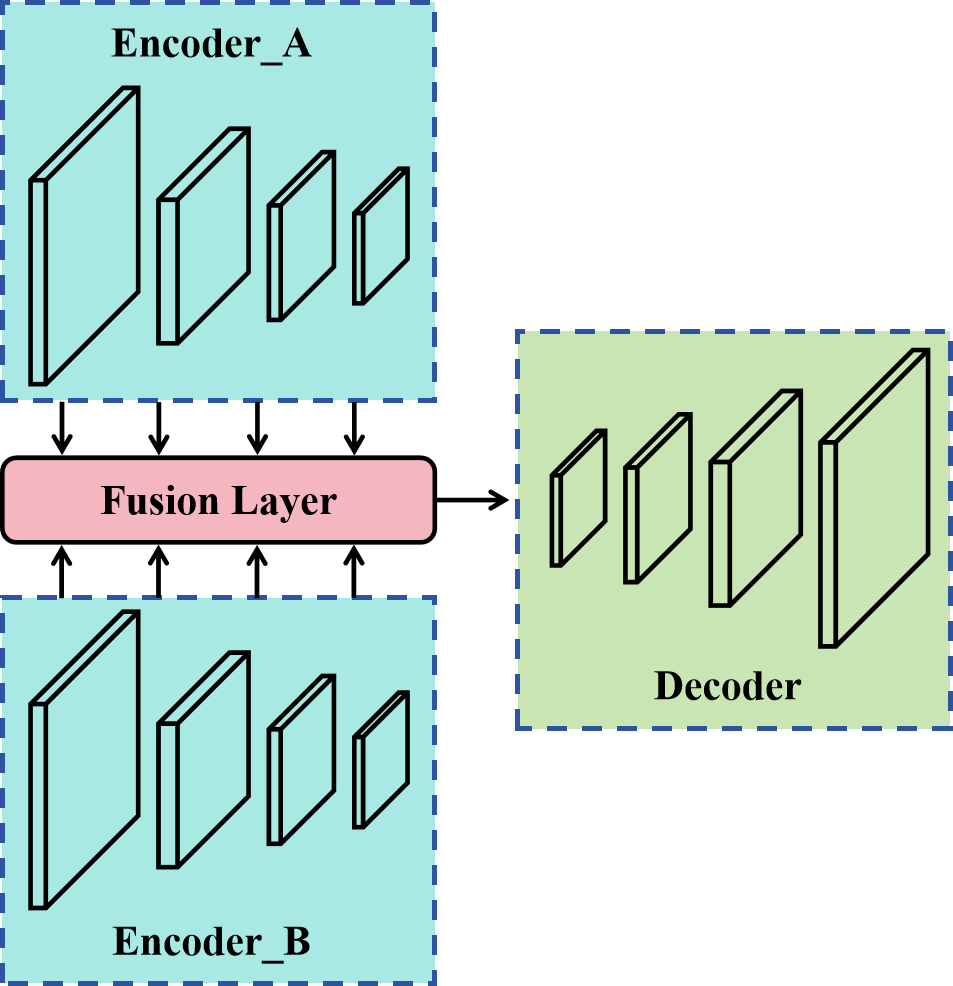
\includegraphics[width=0.6\textwidth]{paper_figures/变化检测任务基础范式设计/SEED1a.png}
  \caption{Siamese 编码器 + 融合 + 解码器。首先,Siamese 编码器提取双时相特征图,然后将这些特征图进行融合,最后对融合后的特征图进行解码。}
  \label{fig:SEED1a}
\end{figure}

%—— 图 b ——
\begin{figure}[!htbp]
  \centering
  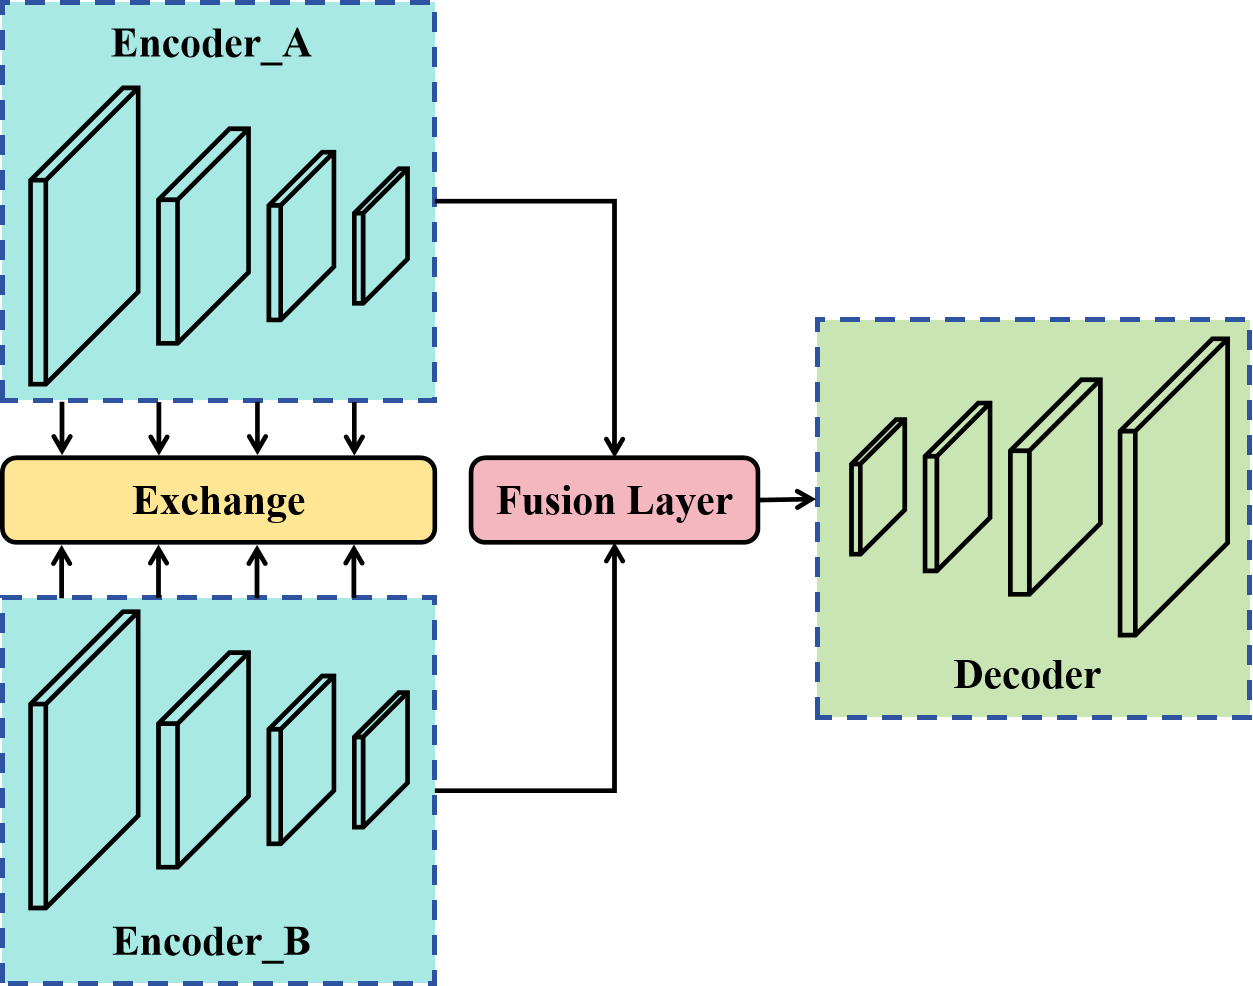
\includegraphics[width=0.6\textwidth]{paper_figures/变化检测任务基础范式设计/SEED1b.png}
  \caption{Siamese 交换(编码器)+ 融合 + 解码器。首先,Siamese 编码器在提取双时相特征图的同时进行特征交换,以增强跨时相的信息交互。交换后的特征图随后进行融合,融合后的特征图最终被解码。}
  \label{fig:SEED1b}
\end{figure}

%—— 图 c ——
\begin{figure}[!htbp]
  \centering
  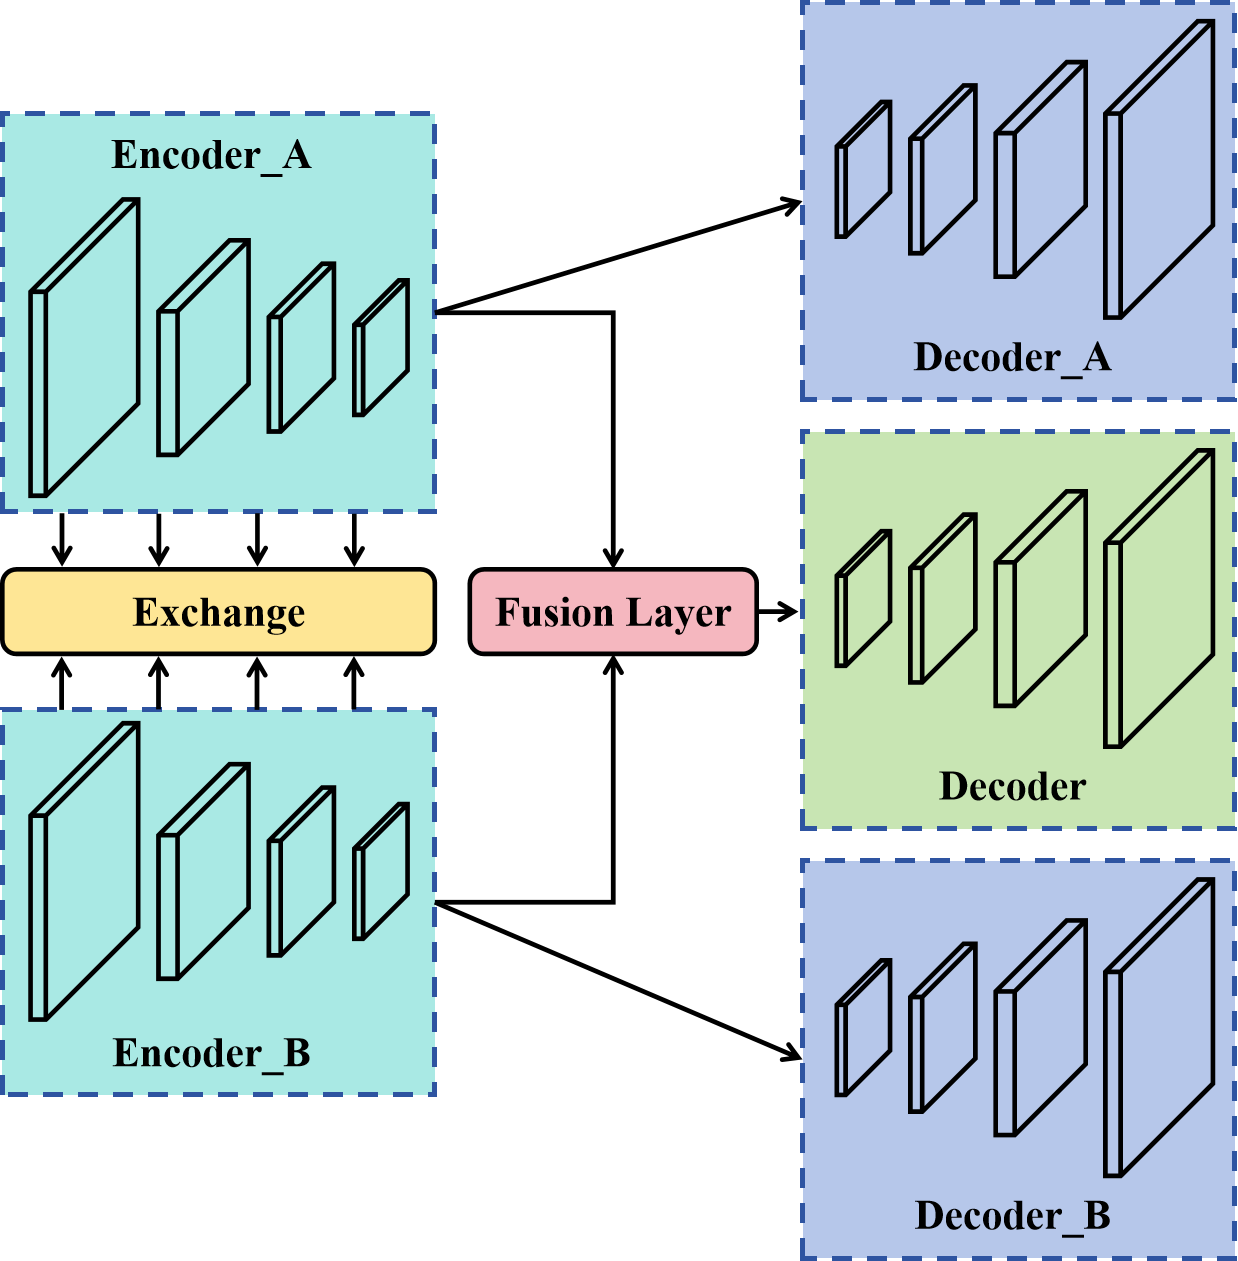
\includegraphics[width=0.6\textwidth]{paper_figures/变化检测任务基础范式设计/SEED1c.png}
  \caption{Siamese 交换(编码器)+ 融合 + 三分支解码器。首先,Siamese 编码器提取双时相特征图,同时进行特征交换,以增强跨时相的信息交互。接下来,交换后的特征图被融合并解码;此外,经过特征交换的 Siamese 编码器分支也被解码。}
  \label{fig:SEED1c}
\end{figure}

%—— 图 d ——
\begin{figure}[!htbp]
  \centering
  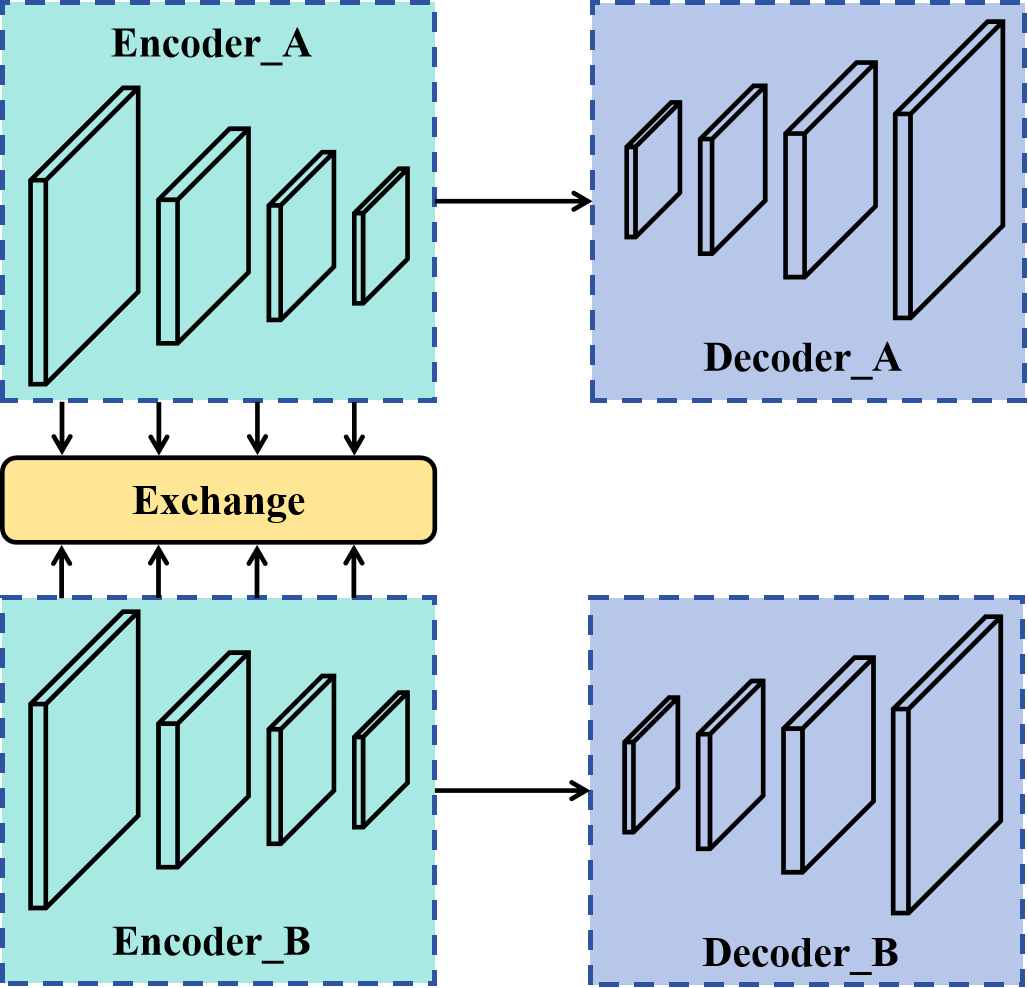
\includegraphics[width=0.6\textwidth]{paper_figures/变化检测任务基础范式设计/SEED1d.png}
  \caption{\textbf{Siamese Encoder-Exchange-Decoder (SEED)}. 首先,Siamese 编码器提取双时相特征图。这些特征图随后被交换,最后对交换后的编码器分支进行解码。}
  \label{fig:SEED1d}
\end{figure}

基于深度学习的变化检测任务的理论基础是,首先利用深度神经网络对双时相影像进行特征提取,然后设计合适的模块来学习差异特征,这些差异特征反映了双时相影像之间的差异~\cite{shi_change_2020,lv_land_2022}。基于这些差异特征,单一解码器能够逐步引导模型识别发生变化的区域。Siamese 神经网络的出现为变化检测任务的特征提取提供了尤为有效的框架~\cite{shi_deeply_2022}。在大多数常用的变化检测模型中,都构建了一个权重共享的特征提取架构。通过该 Siamese 编码器结构,模型可以从双时相影像中提取图像特征,并进一步基于这些双时相特征构建差异特征,以解码变化区域~\cite{zhu_land-useland-cover_2022-1}。


\begin{figure}[!htbp]
  \centering
  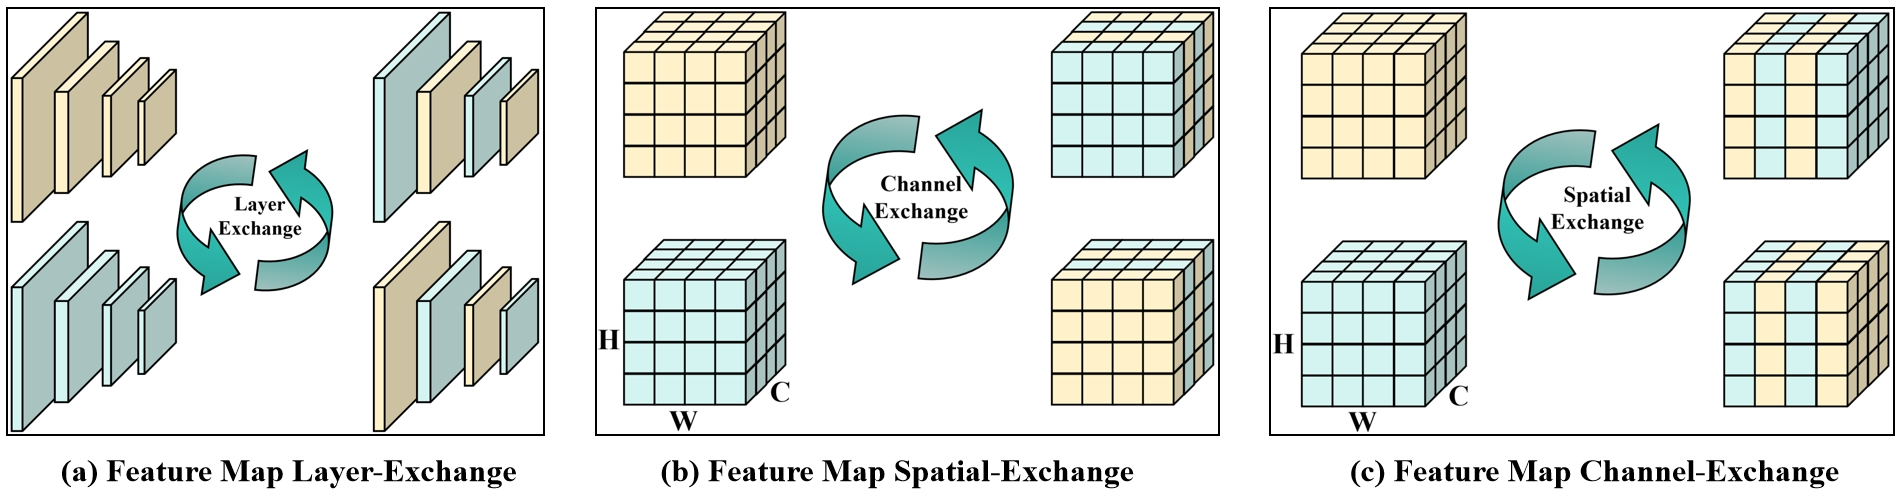
\includegraphics[width=\textwidth]{paper_figures/变化检测任务基础范式设计/seed_exchange.png}
  \caption{三种常见的特征交换方法:层交换、通道交换和空间交换。}
  \label{fig:seed_exchange}
\end{figure}

另一项广泛研究的变化检测内容是差异特征的计算~\cite{pei_feature_2022,x_zhang_difunet_2022,gu2023fdff}。由于变化检测模型以两幅影像作为输入但仅产生单一输出,因此必须在模型内部融合这两幅影像的特征。在常见的变化检测模型中,有三种简单的双时相特征融合方法(Fusion Layer):拼接(concatenation)~\cite{gu2023fdff,wan_d-tnet_2022-3,wang_hmcnet_2022-2}、逐元素相加(element-wise addition)~\cite{pei_feature_2022,gu2023fdff} 和逐元素相减(element-wise subtraction)~\cite{gu2023fdff,shi_deeply_2022,x_zhang_difunet_2022}。拼接方法将双时相特征图在通道维度上堆叠,使模型能够从堆叠后的特征图中学习变化特征;相加方法是一种深度学习中常见的特征融合技术,将两幅特征图逐元素相加,使模型能够从组合特征中提取变化信息;而相减方法则直接计算逐元素差异,以表示变化特征。

然而,利用这类数学运算构建差异特征存在一个根本性问题:这些方法在一定程度上会破坏双时相影像的原始特征。例如,通过相加或相减得到的特征与原始影像特征差异较大,可能会给模型的学习过程带来困难。

为此,研究者们提出了基于特征交换的差异学习方法,并引入了多种以特征交换为核心的范式,如图~\ref{fig:SEED1a}、~\ref{fig:SEED1b}、~\ref{fig:SEED1c}和~\ref{fig:SEED1d}所示。其中,图~\ref{fig:SEED1a} 描绘了经典的基于 Siamese 神经网络的变化检测范式,目前大多数主流变化检测算法即基于此设计;图~\ref{fig:SEED1b} 展示了一个在编码阶段通过特征交换增强双时相影像信息流的特征交换型变化检测框架;图~\ref{fig:SEED1c} 与图~\ref{fig:SEED1b} 类似,只是在解码阶段对交换后的双时相特征图分别进行解码,构建了三分支解码器。从图~\ref{fig:SEED1a}、图~\ref{fig:SEED1b} 和图~\ref{fig:SEED1c} 可以看出,目前的变化检测模型依然依赖 Fusion Layer 来合并双时相特征——因为传统框架普遍认为只有融合双时相特征才能表示变化特征。然而,本章提出了一个新颖的 Siamese Encoder-Exchange-Decoder(SEED)框架。如图~\ref{fig:SEED1d} 所示,SEED 完全摒弃了任何 Fusion Layer,仅依靠特征交换操作。与其他变化检测范式相比,SEED 显得极为简洁。

至于特征交换方法,已有研究者提出了多种基于特征交换的差异方法来改进变化检测模型,主要包括层交换~\cite{dong_efficientcd_2024}、通道交换~\cite{Fang2022ChangerFI,zhao_exchanging_2023} 以及空间交换~\cite{Fang2022ChangerFI,zhao_exchanging_2023},如图~\ref{fig:seed_exchange} 所示。这些方法利用上述三种特征交换技术来加强双时相影像之间的信息交流,从而优化变化检测模型的性能。然而,它们仍然依赖构建差异特征来学习变化区域,尚缺乏对特征交换核心原理的深入分析。

基于前人研究~\cite{dong_efficientcd_2024,Fang2022ChangerFI,zhao_exchanging_2023},可以看出变化检测的核心因素在于:只要保持双时相影像像素对应关系不变,变化检测模型的核心目标就始终是判断每个对应像素在目标类别上是否发生了变化。本章将这一原则称为“像素一致性原则”。基于此洞见,提出了一个简洁的变化检测框架——Siamese Encoder-Exchange-Decoder(SEED)框架。在 SEED 中,完全不计算差异特征,从而在整个模型中保留影像的原始信息。框架仅通过特征交换操作,使模型能在 Siamese 编码器-解码器分支中分别学习变化区域的特征。

在 SEED 框架中,Siamese 编码器共享同一组编码参数,特征交换模块不引入额外参数,Siamese 解码器也共享同一组解码参数。从本质上讲,基于 SEED 框架的变化检测架构仅需一套编码器-解码器参数,在一定程度上将变化检测任务与语义分割任务进行了统一。因此,几乎所有基于编码器-解码器结构的语义分割模型均可直接转化为基于 SEED 框架的变化检测模型。本章的主要贡献可归纳如下:

1. 提出了一种基于特征交换的全新变化检测范式——仅依赖 Siamese 编码器-解码器框架,无需计算任何差异特征,即可识别变化区域。
2. 对特征交换机制进行了深入分析,并通过大量实验验证其可解释性,提出了变化检测任务中的像素一致性原则。
3. SEED 框架实现了变化检测任务与语义分割任务的统一。设计实验证明了,可利用特征交换方法将语义分割模型高效转换为变化检测模型。


\begin{figure}[!htbp]
  \centering
  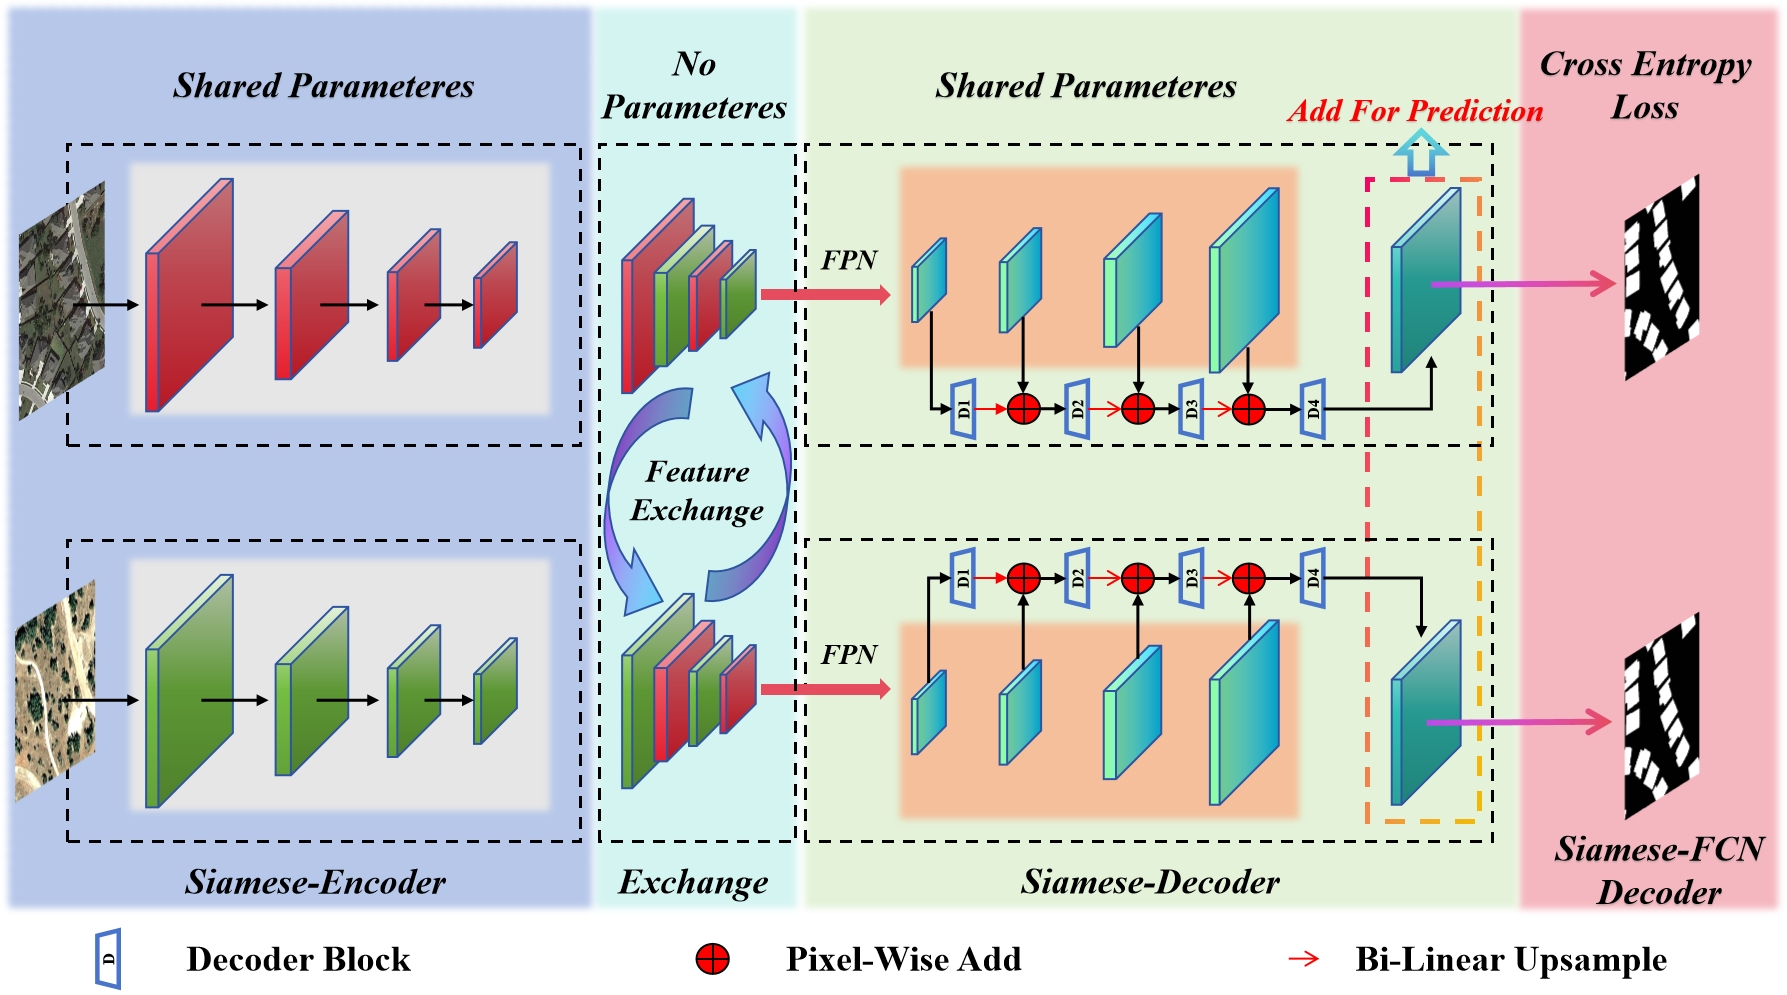
\includegraphics[width=\textwidth]{paper_figures/变化检测任务基础范式设计/SEED_Framework.png}
  \caption{Siamese Encoder-Exchange-Decoder (SEED) 总体架构}
  \label{fig:SEED_Framework}
\end{figure}

\begin{figure}[!htbp]
  \centering
  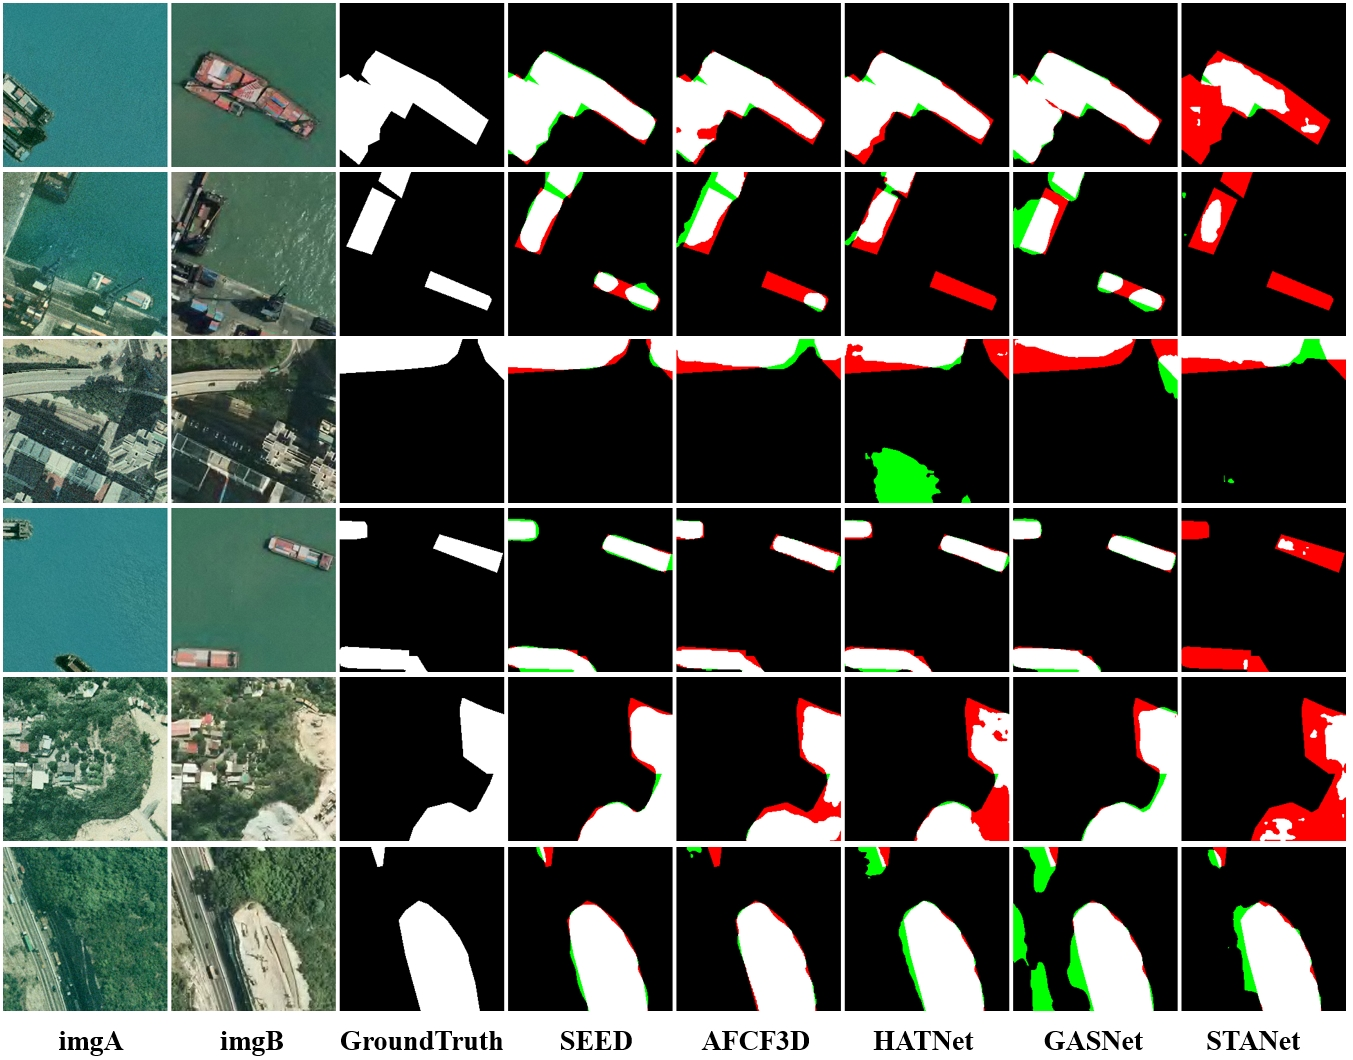
\includegraphics[width=0.8\textwidth]{paper_figures/变化检测任务基础范式设计/seed_sysu.png}
  \caption{ SEED 模型与经典变化检测模型在 SYSU-CD 数据集的可视化对比结果。}
  \label{fig:seed_sysu}
\end{figure}


\begin{table}[!htbp]
\centering
\caption{SEED 模型在 SYSU-CD 数据集上的定量对比结果}
\label{tab:seed_sysu}
\begin{tabular}{lccccc}
\hline
\textbf{Model} & \textbf{OA} & \textbf{IoU} & \textbf{F1} & \textbf{Rec} & \textbf{Prec} \\
\hline
STANet~\cite{chen_spatial-temporal_2020} & 88.24 & 57.22 & 72.79 & 66.71 & 80.08 \\
DSAMNet~\cite{shi_deeply_2022}    & --    & 64.18 & 78.18 & 81.86 & 74.81 \\
P2V~\cite{lin_transition_2023}    & 90.49 & 66.29 & 79.73 & 79.29 & 80.17 \\
RCDT~\cite{lu_cross_2024}         & --    & 67.46 & 80.57 & 86.21 & 75.62 \\
DARNet~\cite{li_densely_2022}     & 91.26 & 68.10 & 81.03 & 79.11 & 83.04 \\
STDF-CD~\cite{y_zhou_stdf_2025}   & 91.42 & 68.83 & 81.53 & 80.35 & 82.76 \\
STFF-GA~\cite{h_wei_spatio-temporal_2024}   & --  & 69.45   & 81.97  & 80.14  & 83.89 \\
SGANet~\cite{j_chen_sganet_2025}  & --    & 69.55 & 82.04 & 76.50 & 88.45 \\
MFCF-Net~\cite{b_huang_remote-sensing_2024}   & 92.05   & 69.79   & 82.21   & 79.37   & 85.25 \\
AMFNet~\cite{zhan_amfnet_2024}     & 92.30  & 69.85 &  82.25 &  82.51 &  88.23 \\
CMCD~\cite{li_cmcd_2025}          & --    & 69.87 & 82.26 & 85.90 & 78.92 \\
MIFNet~\cite{w_xie_mifnet_2025}       & --  & 70.09 & 82.42 & 79.47 & 85.85 \\
\hline
SEED (LE)                             & 92.03 & 70.33 & 82.58 & 80.16 & 85.16 \\
SEED (CE) & 92.16 & 70.91	& 82.98	& 81.01	& 85.05 \\
SEED (SE) & 91.52 & 69.05	& 81.69	& 80.27	& 83.16 \\
\hline
\end{tabular}
\end{table}



\begin{figure}[!htbp]
  \centering
  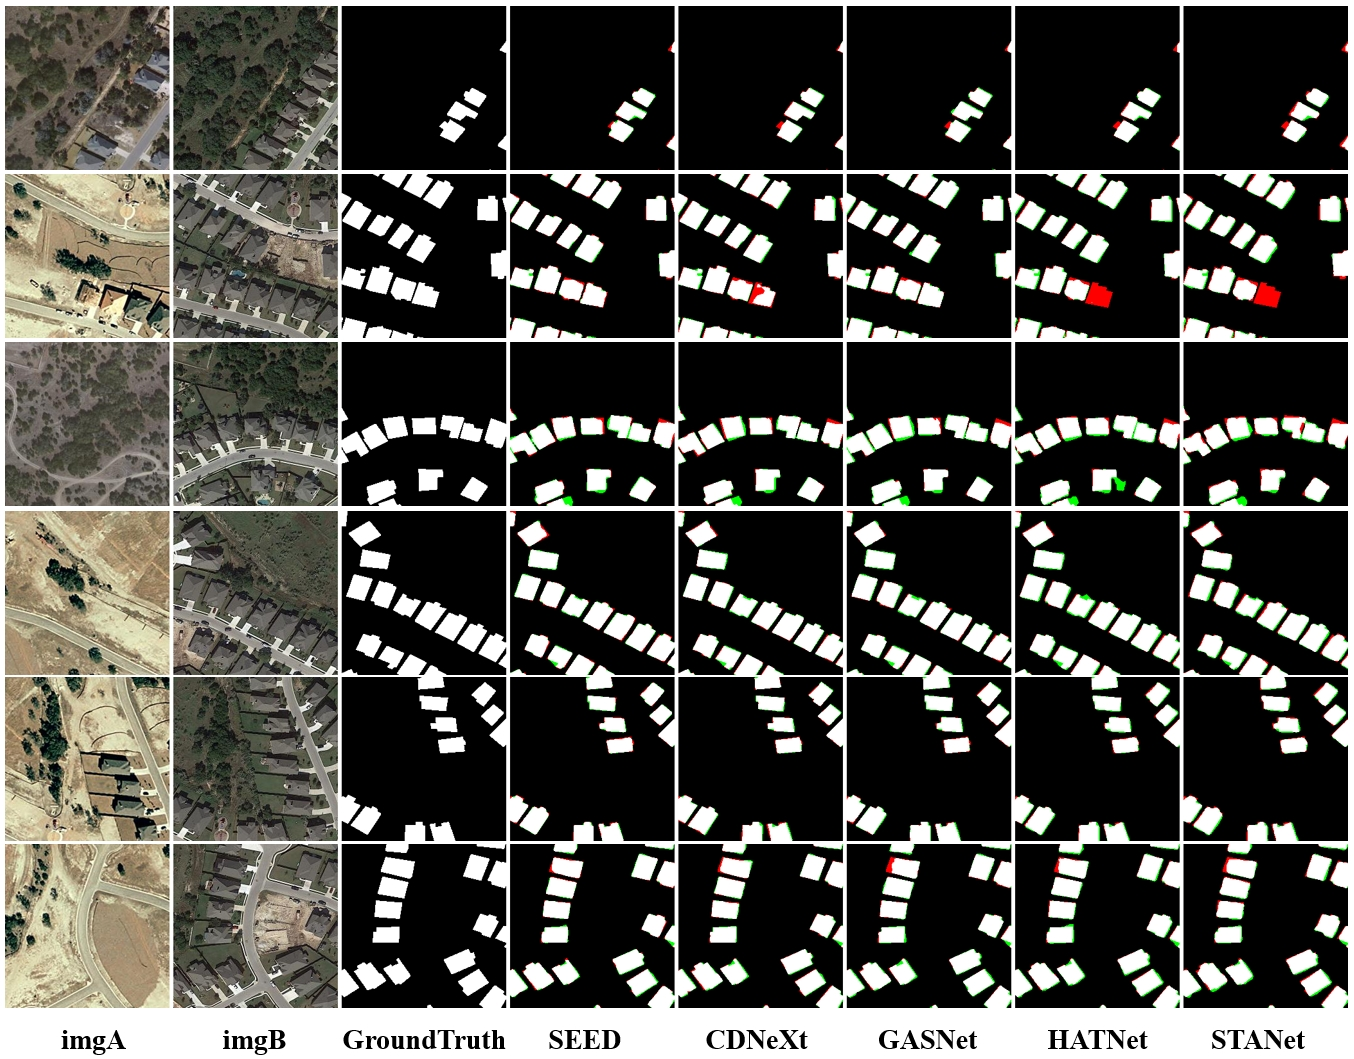
\includegraphics[width=0.8\textwidth]{paper_figures/变化检测任务基础范式设计/seed_levir.png}
  \caption{SEED模型与经典变化检测模型在 LEVIR-CD 数据集的可视化对比结果。}
  \label{fig:seed_levir}
\end{figure}


\begin{table}[!htbp]
\centering
\caption{SEED 模型与经典变化检测模型在 LEVIR-CD 数据集上的定量对比结果}
\label{tab:seed_levir}
\begin{tabular}{lccccc}
\hline
\textbf{Model} & \textbf{OA} & \textbf{IoU} & \textbf{F1} & \textbf{Rec} & \textbf{Prec} \\
\hline
STANet~\cite{chen_spatial-temporal_2020}   & 99.02 & 81.85 & 90.02 & 87.13 & 93.10 \\
CDMamba~\cite{zhang_cdmamba_2025}          & 99.06 & 83.07 & 90.75 & 90.08 & 91.43 \\
AMFNet~\cite{zhan_amfnet_2024}             & 99.07 & 83.13 & 90.79 & 91.15 & 94.77 \\
ISDANet~\cite{h_ren_interactive_2025}      & 99.10 & 83.63 & 91.06 & --    & 92.19 \\
RSM-CD~\cite{zhao_rs-mamba_2024}           & --    & 83.66 & 91.10 & 89.73 & 92.52 \\
DgFA~\cite{f_zhou_dual-granularity_2025}   & 99.11 & 83.93 & 91.26 & 90.84 & 91.69 \\
TRSANet~\cite{j_li_trsanet_2024}           & 99.14 & 84.22 & 91.44 & 89.95 & 92.97 \\
HATNet~\cite{Xu2024HybridAT}             & --    & 84.41 & 91.55 & 90.23 & 92.90 \\
GASNet~\cite{zhang_global-aware_2023}      & 99.11 & --    & 91.21 & 90.62 & 91.82 \\
CMCD~\cite{li_cmcd_2025}                   & --    & 84.50 & 91.60 & 90.48 & 92.74 \\
STFF-GA~\cite{h_wei_spatio-temporal_2024}   & --  & 84.81   & 91.78  & 91.10  & 92.46 \\
MFCF-Net~\cite{b_huang_remote-sensing_2024} & 99.17  & 84.82  & 91.79  & 90.84  & 92.76 \\
STDF-CD~\cite{y_zhou_stdf_2025}            & 99.12 & 85.05 & 91.92 & 91.01 & 92.85 \\
SFFCE-CD~\cite{y_xing_sffce-cd_2025}       & 99.20 & 85.32 & 92.08 & 91.18 & 93.00 \\
MIFNet~\cite{w_xie_mifnet_2025}            & --  & 85.35 & 92.10 & 90.87 & 93.37 \\
SGANet~\cite{j_chen_sganet_2025}           & --    & 85.45 & 92.14 & 91.03 & 93.30 \\
RCDT~\cite{lu_cross_2024}                  & --    & 85.50 & 92.18 & 93.27 & 91.12 \\
FTA-Net~\cite{t_zhu_fta-net_2025}          & --    & 85.58 & 92.23 & 92.68 & 91.79 \\
CDNeXt~\cite{wei_robust_2024}              & 99.24 & 85.86 & 92.39 & 90.92 & 93.91 \\
HASNet~\cite{c_tao_hasnet_2025}            & 99.53 & 85.90 & 92.42 & 92.04 & 92.80 \\
UA-BCD~\cite{li_overcoming_2025}           & --    & 85.99 & 92.47 & 91.57 & 93.38 \\
FTransDF-Net~\cite{li_dual_2025}           & --    & 86.04 & 92.50 & 91.40 & 93.62 \\
RSBuilding~\cite{wang_rsbuilding_2024}     & --    & 86.19 & 92.59 & 91.80 & 93.39 \\
\hline
SEED (LE)                                      & 99.26 & 86.25 & 92.62 & 90.97 & 94.32 \\
SEED (CE) & 99.25	& 86.03	& 92.49	& 91.08	& 93.94 \\
SEED (SE) & 99.26	& 86.24	& 92.61	& 91.42	& 93.83 \\
\hline
\end{tabular}
\end{table}

\section{SEED架构设计方法}
\subsection{整体架构}  
本工作主要探讨变化检测任务的框架设计~\cite{dong_efficientcd_2024, Fang2022ChangerFI, zhao_exchanging_2023},提出了 Siamese Encoder-Exchange-Decoder(SEED)框架,如图~\ref{fig:SEED_Framework} 所示。在 SEED 框架的编码阶段,基于 SwinTv2-Base~\cite{liu_swin_2021-5}、EfficientNet-B4~\cite{tan_efficientnet_2019} 和 ResNet50~\cite{He2015DeepRL} 构建了权重共享的 Siamese 编码器。在特征交换阶段,采用了三种不同的交换方式:特征图层交换、特征图通道交换和特征图空间交换。在颈部阶段,使用参数共享的特征金字塔网络(FPN)~\cite{lin_feature_2017} 对交换后的双时相特征金字塔进行处理。在解码阶段,为了充分验证 SEED 框架的潜力,构建了一个极其简洁的逐层解码结构,并共享解码器参数。此外,对于 SwinTv2 主干网络,在解码器中集成了简单的 Swin Transformer V2 模块以优化特征;而对于 EfficientNet 和 ResNet,则采用 ResNet 的 BottleNeck 模块进行特征优化。在训练阶段,解码器的两个分支分别计算损失;在推理阶段,将两个分支的预测结果相加并取平均,作为变化检测模型的最终输出。

\subsection{特征交换方法}  
在前人工作~\cite{dong_efficientcd_2024, Fang2022ChangerFI, zhao_exchanging_2023}的基础上,本章深入研究了三种特征交换方案,并通过实验结果验证了变化检测任务中的像素一致性定理。首先,这些方案在不引入任何额外可学习参数的条件下,即可促进双时相影像间的特征信息交互,增强模型对双时相数据的理解;其次,基于这些特征交互的框架摒弃了复杂的差异特征计算,使模型在保留原始特征完整性的同时,学习到有效的变化特征。以下分别介绍这三种方案。

\subsubsection{特征图层交换(Layer-Exchange, LE)}
特征图层交换在层级维度上进行特征交换,如图~\ref{fig:seed_exchange}(a) 所示。给定来自双时相影像的两组特征列表 \(\{x_i\}\) 和 \(\{y_i\}\),按照预设步长(例如每隔一层)交换对应层的特征。具体而言,假设特征列表为 \(\{x_0, x_1, x_2, x_3\}\) 与 \(\{y_0, y_1, y_2, y_3\}\),则以步长 \(2\) 交换 \(x_0 \leftrightarrow y_0\)、\(x_2 \leftrightarrow y_2\),其余层保持不变。

\subsubsection{特征图通道交换(Channel-Exchange, CE)} 
特征图通道交换按固定规则交换通道,如图~\ref{fig:seed_exchange}(b) 所示。例如,在通道交换中,依据预设步长(如 $2$)选择部分通道进行交换。假设共有 $C$ 个通道,则依次交换通道索引为 $0,2,4,\ldots$ 的通道与另一路分支的对应通道,其余通道保持不变。


\begin{figure}[!htbp]
  \centering
  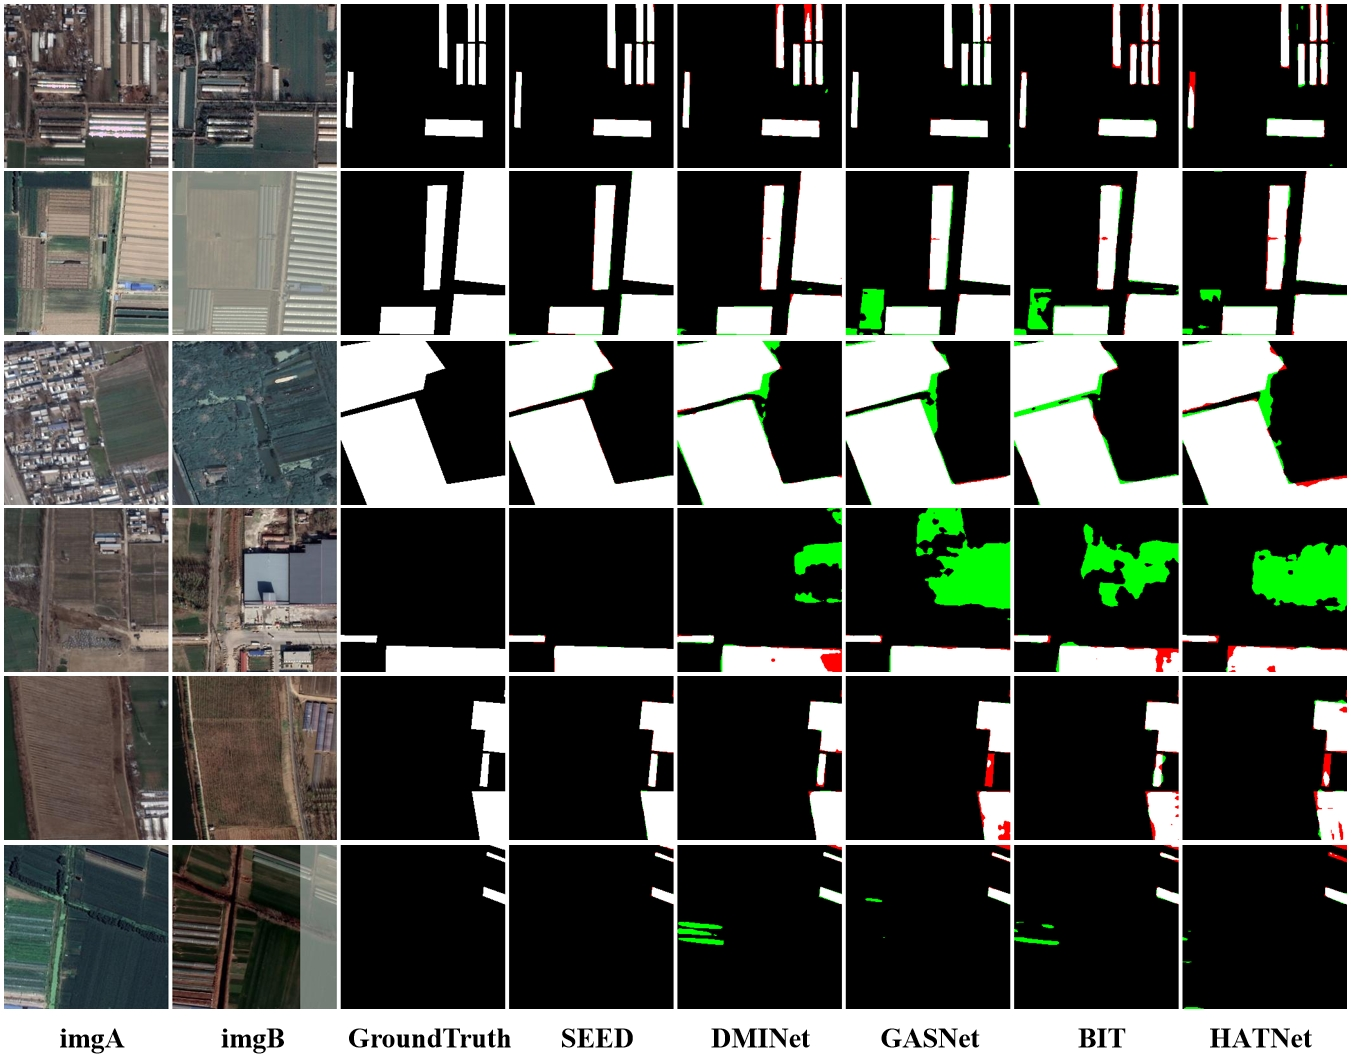
\includegraphics[width=0.8\textwidth]{paper_figures/变化检测任务基础范式设计/seed_pxclcd.png}
  \caption{SEED 模型与经典变化检测模型在 PX-CLCD 数据集的可视化对比结果。}
  \label{fig:seed_pxclcd}
\end{figure}

\subsubsection{特征图空间交换(Spatial-Exchange, SE)}
特征图空间交换在空间维度上进行特征交换,如图~\ref{fig:seed_exchange}(c) 所示。具体而言,给定双时相影像的两幅特征图,按照预设步长(例如 $2$)在宽度(或高度)方向上按指定间隔将特征图划分为若干列(或行),并交换两幅特征图中对应的列(或行)。


\begin{table}[!htbp]
\centering
\caption{SEED 模型与经典变化检测模型在 PX-CLCD 数据集上的定量对比结果}
\label{tab:seed_pxclcd}
\begin{tabular}{lccccc}
\hline
\textbf{Model} & \textbf{OA} & \textbf{IoU} & \textbf{F1} & \textbf{Rec} & \textbf{Prec} \\
\hline
HANet~\cite{Han2024HANetAH}         & 98.50 & 88.99 & 94.18 & 93.83 & 94.53 \\
MSCANet~\cite{m_liu_cnn-transformer_2022}       & 98.50 & 89.00 & 94.18 & 93.95 & 94.41 \\
DDAM-Net~\cite{feng_ddam-net_2024} & -- & 90.70 & 95.12 & 94.78 & 95.47 \\
BIT~\cite{chen_remote_2022}           & 98.76 & 90.78 & 95.17 & 94.80 & 95.54 \\
GASNet~\cite{zhang_global-aware_2023}    & 98.99 & 92.51 & 96.11 & 96.42 & 95.80 \\
DMINet~\cite{feng_change_2023}         & 99.04 & 92.83 & 96.28 & 96.31 & 96.25 \\
SNUNet3+~\cite{miao_snunet3_2024}     & 99.19 & 93.61 & 96.64 & 96.79 & 96.60 \\
CGNet~\cite{han_change_2023}         & 99.17 & 93.82 & 96.81 & 97.33 & 96.30 \\
\hline
SEED (LE)          & 99.38 & 95.34 & 97.61 & 97.46 & 97.76 \\
SEED (CE)          & 99.40	& 95.50	& 97.70	& 98.07	& 97.33 \\
SEED (SE)          & 99.32 & 94.86 & 97.36 & 96.89 & 97.84 \\
\hline
\end{tabular}
\end{table}

\subsubsection{随机交换(Random Exchange)}
为了进一步验证特征交换方法的有效性及像素一致性原则在变化检测任务中的正确性,在上述三种特征交换方法的基础上引入随机性,提出了一种随机交换策略,以在训练过程中实现更丰富的特征混合。具体而言,随机交换不再按照固定规则(如固定步长或索引)进行特征交换,而是基于一定的概率或随机选择策略,在不同层级、通道或空间位置有选择地交换特征,具体如下:

\textbf{随机层交换(Random Layer Exchange, RLE)}: 对每一层生成一个随机数;若该随机数小于给定阈值(例如 0.5),则交换对应层的特征,否则保持不变。

\textbf{随机通道交换(Random Channel Exchange, RCE)}: 首先随机打乱通道索引,然后按一定比例(例如 0.5)选择部分通道进行交换,其余通道保持不变。

\textbf{随机空间交换(Random Spatial Exchange, RSE)}: 在空间维度上,对每个位置(如列或行)生成一个随机数,并以一定概率(例如 0.5)决定是否交换该位置的特征。  



\begin{figure}[!htbp]
  \centering
  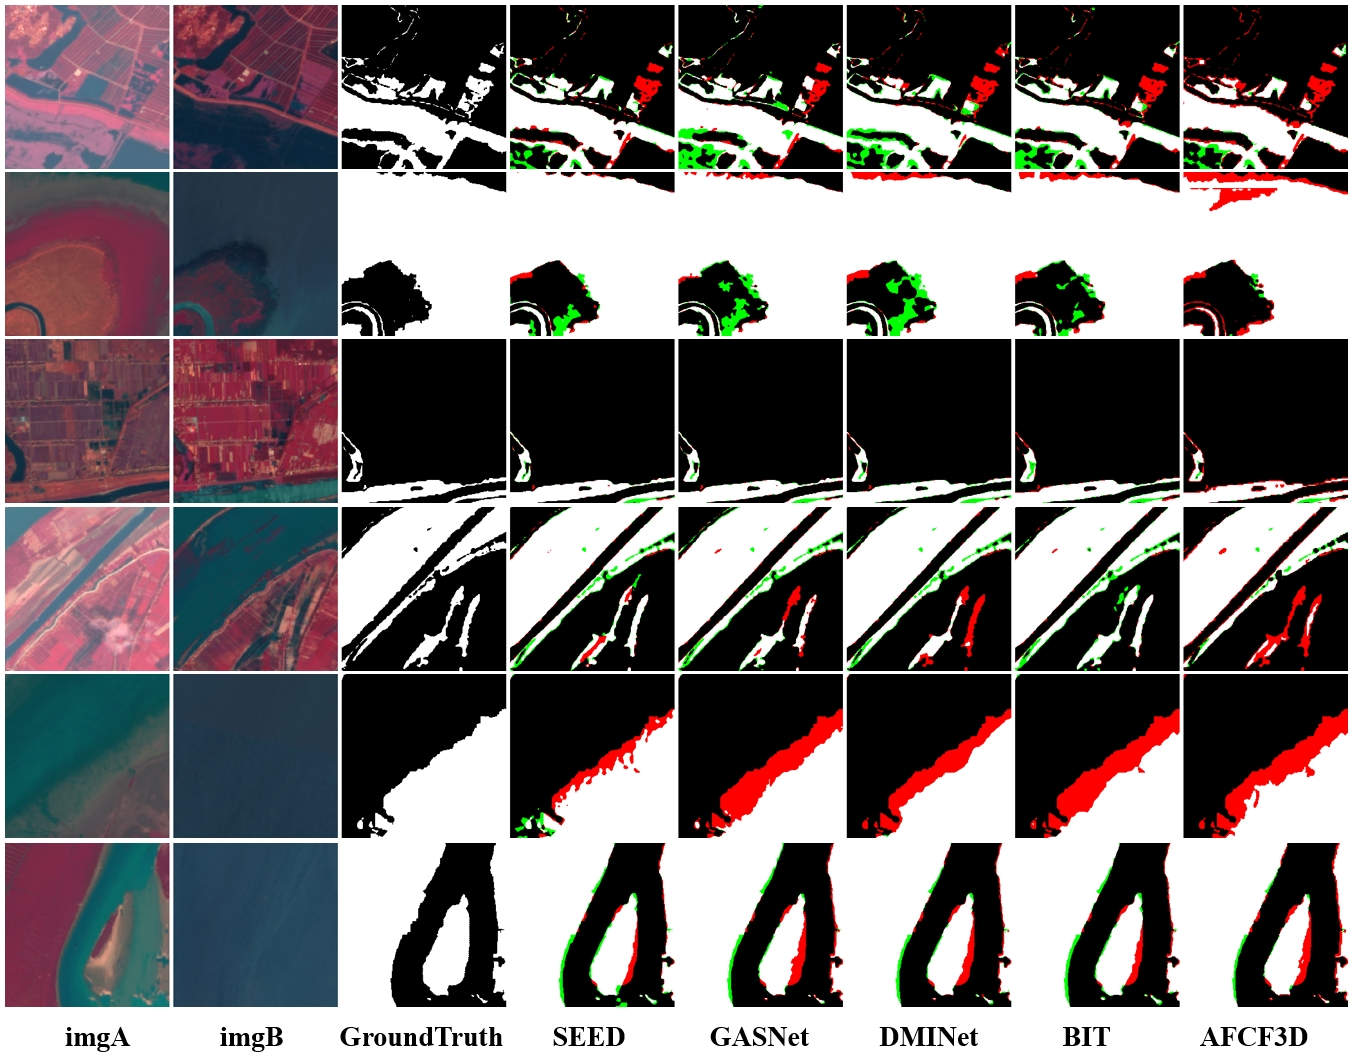
\includegraphics[width=0.8\textwidth]{paper_figures/变化检测任务基础范式设计/seed_watercd.png}
  \caption{SEED 模型与经典变化检测模型在 Water-CD 数据集的可视化对比结果}
  \label{fig:seed_watercd}
\end{figure}

使用上述特征交换方案进行了大量实验。结果表明,这些方案均未对变化检测模型的性能产生负面影响。在随机交换实验中,传统计算机视觉通常将通道信息与语义内容关联、将空间信息与纹理关联,因此对其进行更改时往往需要谨慎。然而在变化检测任务中,可以按照特定规则交换特征图,甚至采用随机交换策略。这一现象验证了变化检测任务中的像素一致性原则。实验结果表明,基于深度学习的变化检测模型并不依赖于构建差异特征,而是通过特征交换直接从双时相特征中学习变化区域的特征。


\begin{table}[!htbp]
\centering
\caption{SEED 模型与经典变化检测模型在 Water-CD 数据集上的定量对比结果}
\label{tab:seed_watercd}
\begin{tabular}{lccccc}
\hline
\textbf{Model} & \textbf{OA} & \textbf{IoU} & \textbf{F1} & \textbf{Rec} & \textbf{Prec} \\
\hline
AFCF3DNet~\cite{ye_adjacent-level_2023} & 95.63 & 77.06 & 87.04 & 80.17 & 95.20 \\
HANet~\cite{Han2024HANetAH}    & 95.94 & 79.94 & 88.85 & 88.34 & 89.37 \\
ELGCNet~\cite{m_noman_elgc-net_2024}   & 96.14 & 80.79 & 89.37 & 88.60 & 90.16 \\
BIT~\cite{chen_remote_2022}           & 96.52 & 82.52 & 90.42 & 89.55 & 91.31 \\
DMINet~\cite{feng_change_2023}         & 96.55 & 82.67 & 90.51 & 89.87 & 91.17 \\
GASNet~\cite{zhang_global-aware_2023}    & 96.72 & 83.48 & 91.00 & 90.41 & 91.59 \\
CDNeXt~\cite{wei_robust_2024}        & 96.88 & 84.21 & 91.43 & 90.71 & 92.15 \\
TRSANet~\cite{j_li_trsanet_2024}     & 97.01 & 84.69 & 91.71 & 90.22 & 93.25 \\
\hline
SEED (LE)          & 96.98 & 84.64 & 91.68 & 90.69 & 92.69 \\
SEED (CE) & 96.94	& 84.43	& 91.56	& 90.64	& 92.50 \\
SEED (SE) & 96.86	& 84.06	& 91.34	& 90.42	& 92.27 \\
\hline
\end{tabular}
\end{table}


\subsection{孪生-编码-交换-解码(SEED)框架设计原理}
尽管在语义分割任务中,特征交换方案可能会破坏图像特征,但在变化检测任务中,只要双时相影像中成对像素的空间对应关系得以保持,无论如何交换特征,模型的学习目标均保持不变。本章将双时相影像中对应像素对的空间关系保持称为“像素一致性原则”。换言之,只要遵循像素一致性原则,任何形式的特征交换都不会影响变化检测模型的基本性能。因此,在保持像素一致性的前提下,可基于多种特征交换规则设计灵活的变化检测模型。  


\begin{figure}[!htbp]
  \centering
  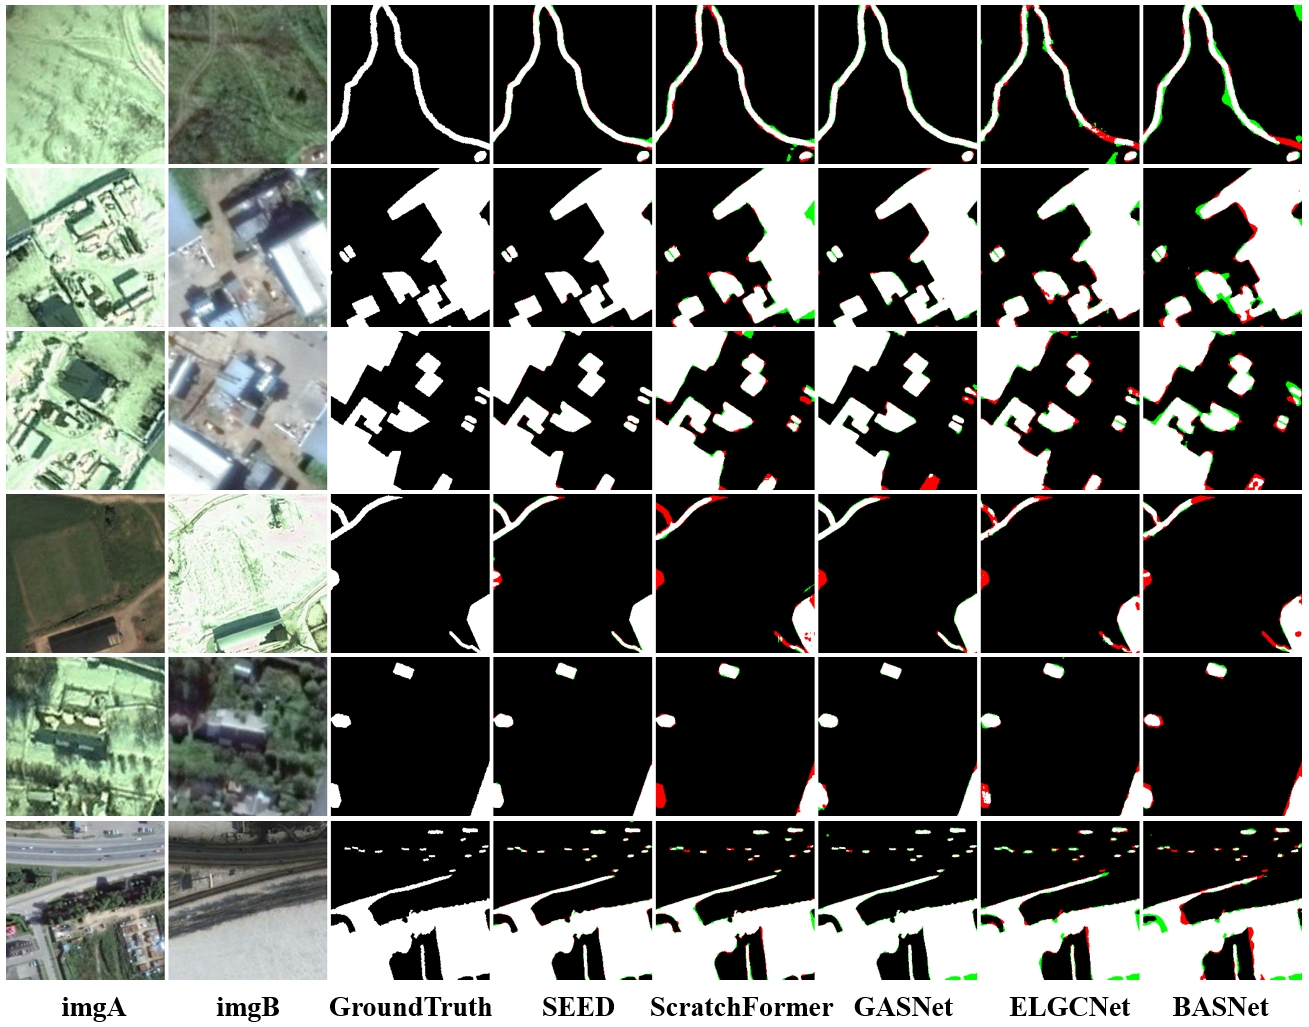
\includegraphics[width=0.8\textwidth]{paper_figures/变化检测任务基础范式设计/seed_cdd.png}
  \caption{SEED 模型与经典变化检测模型在 CDD 数据集的可视化对比结果}
  \label{fig:seed_cdd}
\end{figure}

基于上述特征,设计了如图~\ref{fig:SEED_Framework} 所示的方案。采用常见的主干网络作为编码器进行特征提取,并实现了权重共享的双分支结构。特征提取完成后,加入特征交换阶段,并分别对前文讨论的三种特征交换方案进行实验验证。随后,将经过特征交换的双时相特征金字塔输入参数共享的特征金字塔网络(FPN)进行进一步处理。FPN 模块通过融合与信息交换,实现了双分支特征金字塔的全面融合,等效地将两条分支转换为两组等价的特征金字塔序列。最后,基于这两组特征金字塔,设计了一个基于逐层上采样的简单特征融合解码器作为基础解码方案。此外,由于经过特征交换后 FPN 处理的双时相特征金字塔在本质上是等价的,因此在解码阶段同样采用了参数共享的解码器。基于上述 SEED 框架的构建,仅使用一套编码器—解码器参数,即可构建出高性能的变化检测模型。  


\begin{table}[!htbp]
\centering
\caption{SEED 模型与经典变化检测模型在 CDD 数据集上的定量对比结果}
\label{tab:seed_cdd}
\begin{tabular}{lccccc}
\hline
\textbf{Model} & \textbf{OA} & \textbf{IoU} & \textbf{F1} & \textbf{Rec} & \textbf{Prec} \\
\hline
BASNet~\cite{z_wang_bitemporal_2024} & 99.18 & 93.29 & 96.53 & 96.30 & 96.76 \\  
UA-BCD~\cite{li_overcoming_2025}     & --    & 93.49 & 96.64 & 96.90 & 96.38 \\
RCDT~\cite{lu_cross_2024}                  & --    & 93.79 & 96.80 & 96.97 & 96.63 \\
CDMamba~\cite{zhang_cdmamba_2025}    & 99.26 & 93.93 & 96.87 & 96.84 & 96.90 \\
SFFCE-CD~\cite{y_xing_sffce-cd_2025}   & 99.29 & 94.42 & 97.13 & 96.94 &  97.32 \\
ELGCNet~\cite{m_noman_elgc-net_2024}   & 99.33  &  94.50   & 91.17  & --   & -- \\   
DgFA~\cite{f_zhou_dual-granularity_2025} & 99.41 & 95.12 & 97.50 & 97.60 & 97.40 \\
GASNet~\cite{zhang_global-aware_2023}  & 99.41  & 95.34  & 97.61  & 98.06  & 97.17 \\
MLDFNet~\cite{d_sidekejiang_mldfnet_2025}  & -- & 95.78 & 97.84 & 97.97 & 97.72 \\
ScratchFormer~\cite{Noman2023RemoteSC}   & 99.50 & 95.85  & 97.88 & -- & -- \\ 
FTransDF-Net~\cite{li_dual_2025}   & -- & 95.85 &  97.88 & 97.63 & 98.13 \\
DSFI-CD~\cite{x_li_dsfi-cd_2025}  & 99.52 & 96.10 &  98.01 & 98.34 & 97.68 \\
HASNet~\cite{c_tao_hasnet_2025}        & 99.56 & 96.49 & 98.21 & 98.12 & 98.32 \\
\hline
SEED (LE)                               & 99.64	& 97.11	& 98.53	& 98.44	& 98.63 \\
SEED (CE) & 99.59	& 96.75	& 98.35	& 98.36	& 98.34 \\
SEED (SE) & 99.55	& 96.40	& 98.17	& 98.02	& 98.32 \\
\hline
\end{tabular}
\end{table}


\section{实验结果与分析}

\subsection{实验结果量化指标与可视化分析}
在本章中,对 SEED 架构与最先进的变化检测算法进行了详细的对比实验。表中所有 SEED 的结果均基于 Swin Transformer V2 主干网络。正如表~\ref{tab:seed_sysu}、表~\ref{tab:seed_levir}、表~\ref{tab:seed_pxclcd}、表~\ref{tab:seed_watercd}和表~\ref{tab:seed_cdd} 所示,SEED 框架在SYSU-CD、LEVIR-CD、PX-CLCD、Water-CD 以及 CDD数据集上均表现优异,充分展示了其有效性和鲁棒性。此外,无论是层交换(LE)、通道交换(CE)还是空间交换(SE),SEED 架构的各项准确率指标均十分出色,进一步验证了特征交换方法的合理性。


\begin{figure}[!htbp]
    \centering
    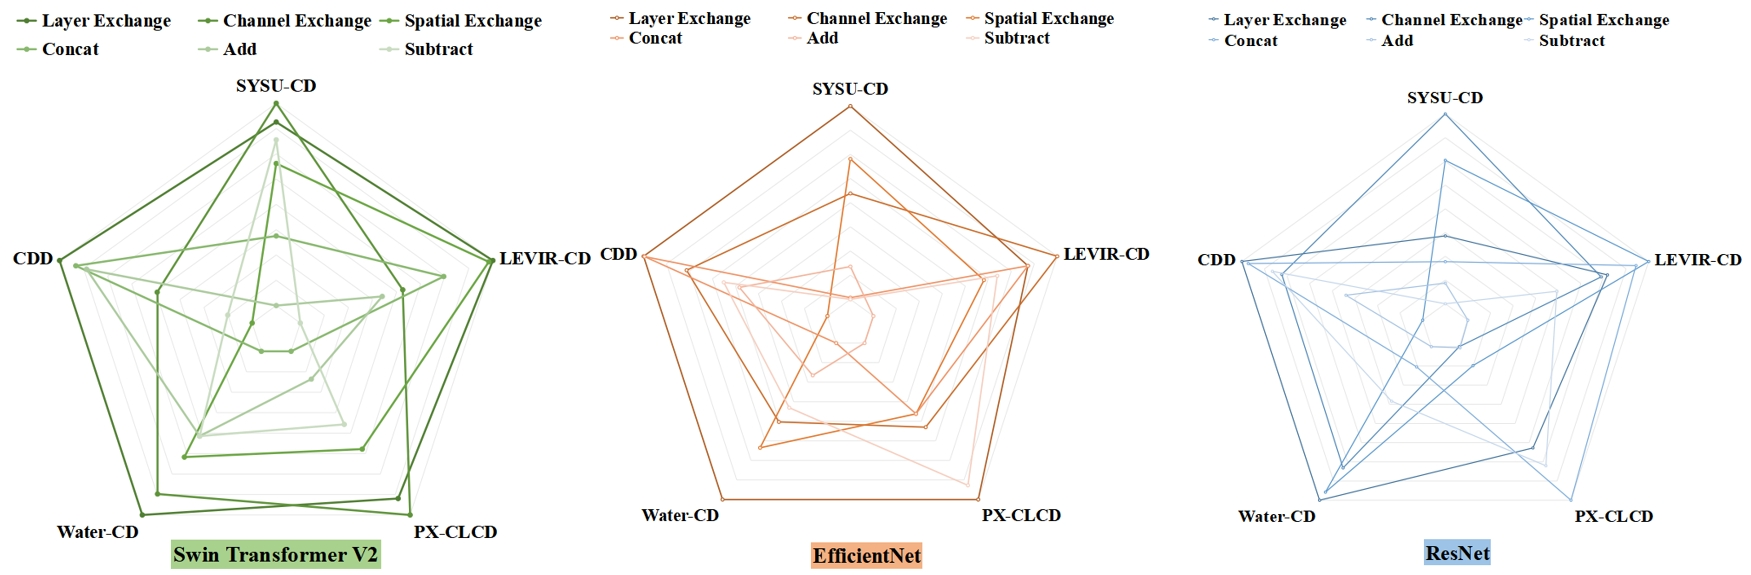
\includegraphics[width=\textwidth]{paper_figures/变化检测任务基础范式设计/seed_rader_image.png} % 
    \caption{基于IoU指标的SEED 架构配合不同特征交换方法在变化检测数据集上的对比结果}
    \label{fig:seed_rader_image}
\end{figure}

首先,在 SYSU‐CD 数据集上,SEED 模型实现了 92.16\% 的整体准确率(OA)和 70.91\% 的 IoU,F1 分数为 82.98\%。这不仅显著超过了 DSAMNet、P2V、DARNet 和 STDF‐CD 等模型,而且在 Recall 与 Precision 上表现均衡,表明 SEED 即使在复杂场景中也能有效捕捉双时相影像中的细微变化。

其次,在以建筑变化检测为主的 LEVIR‐CD 数据集上,大多数模型已取得较高分数,但 SEED 仍以 99.26\% 的 OA 和 86.25\% 的 IoU 排名第一。与在更大建筑数据集上训练的 RSBuilding 模型相比,SEED 在 F1 与 Precision 上虽优势有限却稳定,展现了其在建筑变化检测任务中准确识别变化区域的卓越能力。

在以耕地变化检测为主且需要提取细节的 PX‐CLCD 数据集上,SEED 模型取得了 99.40\% 的 OA、95.50\% 的 IoU 以及 97.70\% 的 F1 分数,远超 SNUNet3+、CGNet 等其他模型。该结果证明 SEED 框架具备更强的细节提取与区分能力,更加适用于复杂耕地变化检测场景。  


\begin{figure}[!htbp]
    \centering
    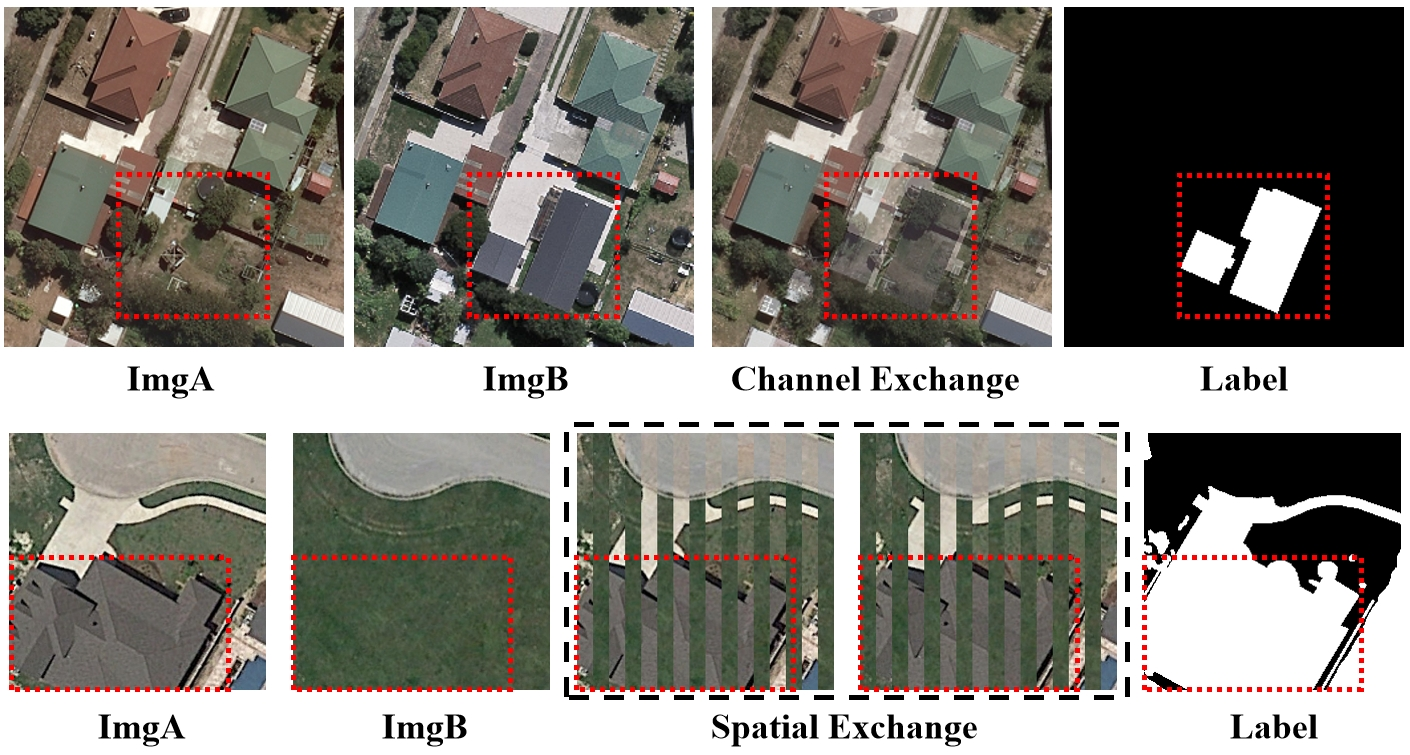
\includegraphics[width=\textwidth]{paper_figures/变化检测任务基础范式设计/seed_exchange_vis.png} % 
    \caption{针对于原始图像的特征交换的可视化结果,突出显示了变化区域。}
    \label{fig:seed_exchange_vis}
\end{figure}

\begin{figure}[!htbp]
  \centering
    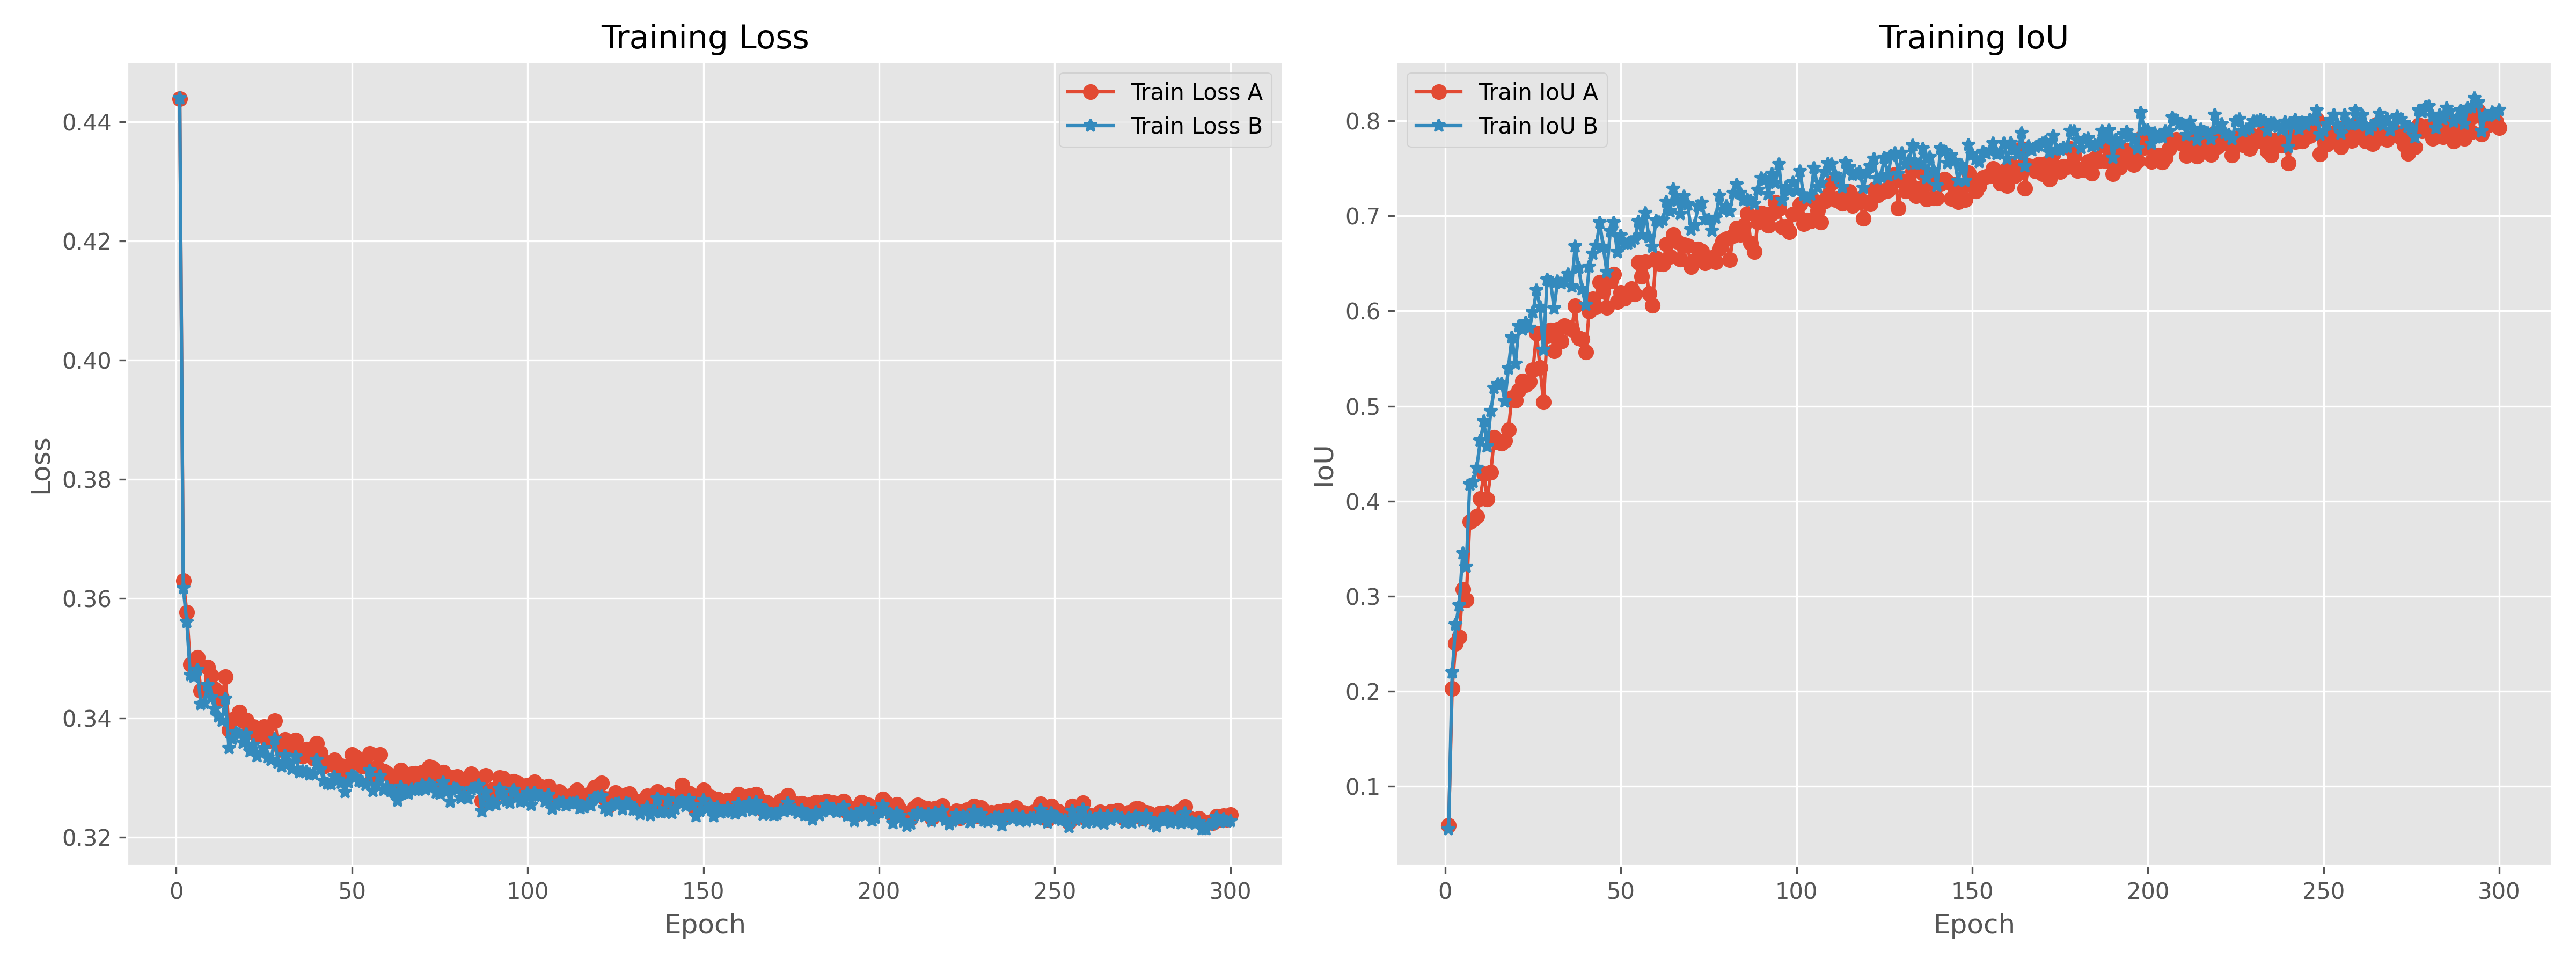
\includegraphics[width=0.8\textwidth]{paper_figures/变化检测任务基础范式设计/chanel_training_log.png} % 
    \caption{基于通道交换的训练日志}
    \label{fig:chanel_training}
\end{figure}
  
\begin{figure}[!htbp]
    \centering
    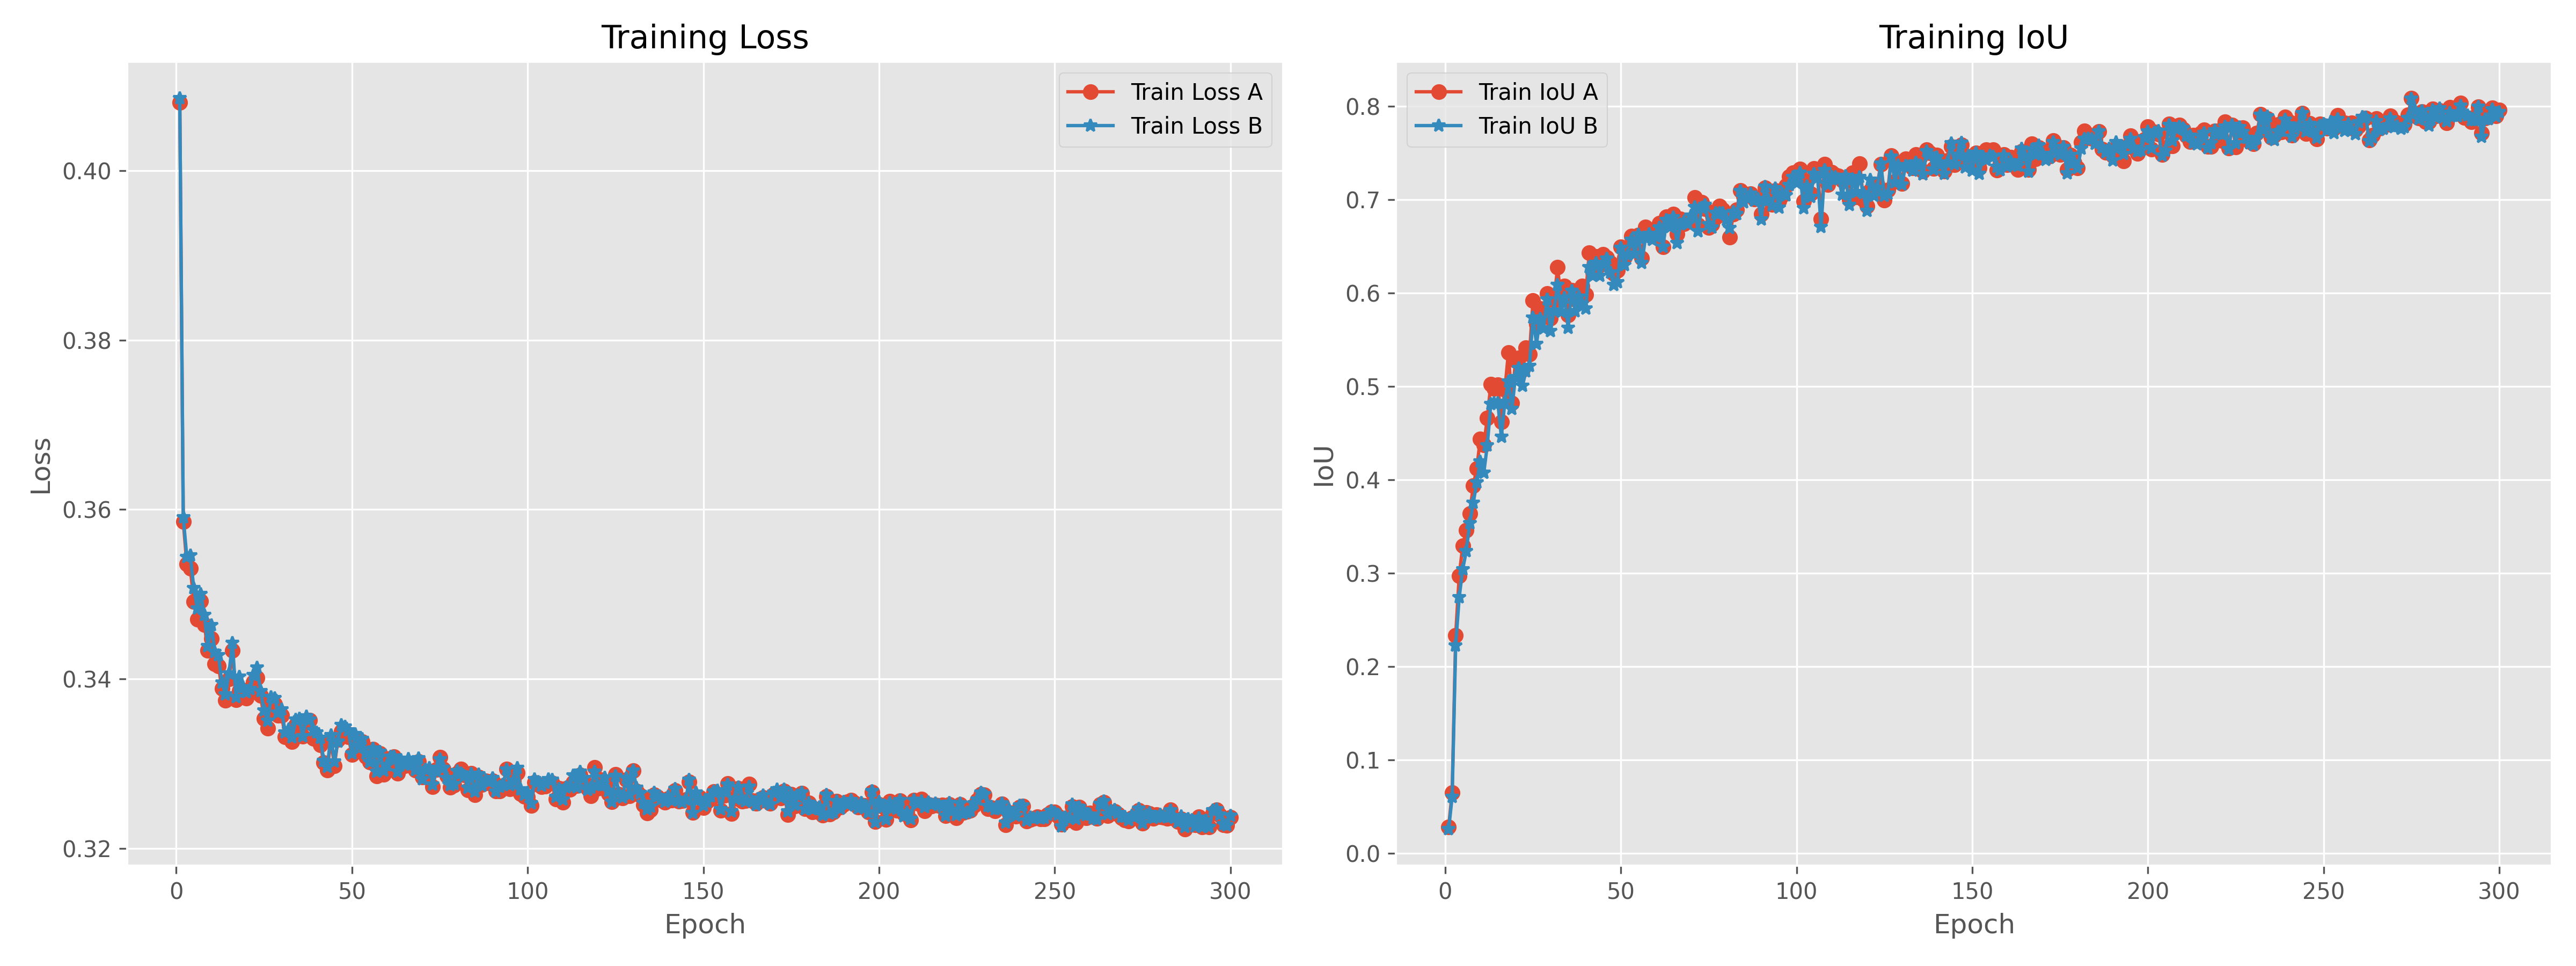
\includegraphics[width=0.8\textwidth]{paper_figures/变化检测任务基础范式设计/spatial_training_log.png} % 
    \caption{基于空间交换的训练日志}
    \label{fig:spatial_training}
\end{figure}

首先,在 Water-CD 数据集上,SEED 模型仍取得了 96.98\% 的整体准确率(OA)和 84.64\% 的 IoU,F1 分数为 91.68\%,在所有指标上均超越了 AFCF3DNet、HANet 和 ELGCNet 等方法。这表明 SEED 框架能够有效处理水资源变化检测中固有的复杂特征,具有很高的实用价值。

最后,在面向季节变化且需要高精度捕捉细微连续变化的 CDD 数据集上,SEED 模型表现卓越,以 99.64\% 的 OA、97.11\% 的 IoU 和 98.53\% 的 F1 分数领先所有对比模型,展现了极高的检测准确性和稳定性。

总体而言,SEED 框架通过摒弃传统的差异特征计算方法,而将特征交换与简洁的编码器–解码器结构相结合,不仅在各类场景和数据集上取得了优异性能,还在建筑变化、耕地变化、水资源变化和季节变化等应用中展现了强大的适应性和鲁棒性。这些实验结果充分验证了特征交换策略在变化检测任务中的有效性。

此外,图~\ref{fig:seed_sysu}、图~\ref{fig:seed_levir}、图~\ref{fig:seed_pxclcd}、图~\ref{fig:seed_watercd}和图~\ref{fig:cdd} 展示了 SEED 模型在 SYSU-CD、LEVIR-CD、PX-CLCD、Water-CD 和 CDD 等五个数据集上的测试结果可视化。这些数据集代表了多种变化检测场景:SYSU-CD 涵盖多目标变化,LEVIR-CD 主要关注建筑物变化,PX-CLCD 强调耕地变化,Water-CD 聚焦水体变化,而 CDD 则反映季节性变化特征。在这些可视化图像中,真阳性(TP)以白色像素表示,真阴性(TN)以黑色像素表示,假阳性(FP)以绿色像素表示,假阴性(FN)以红色像素表示。直观的可视化结果表明,SEED 模型能够在多种场景中准确捕捉变化区域,其检测结果与真实标注高度一致,不仅具有极高的检测精度,还展现了出色的鲁棒性和稳定性。这些丰富的可视化进一步验证了 SEED 框架在处理各类变化类型和复杂环境中的卓越性能。

\subsection{消融研究}
在本章中,提出了一种新颖的变化检测框架——SEED 架构。该框架完全摒弃了变化检测任务中常用的差异特征计算模块,而仅在双时相特征金字塔上应用特征交换。如表~\ref{tab:seed_sysu_backbone} 至表~\ref{tab:seed_cdd_backbone} 所示,在 SYSU-CD、LEVIR-CD、PX-CLCD、Water-CD 和 CDD 数据集上进行了实验。特征提取阶段,分别采用 Swin Transformer V2、EfficientNet-B4 和 ResNet50 作为主干网络;特征交换阶段,依次应用了层交换、通道交换和空间交换三种方法;解码设计中,对于基于 Swin Transformer V2 的主干,使用 Swin Transformer Block 构建解码器;对于 EfficientNet-B4 与 ResNet50 主干,采用 ResNet 的 BottleNeck 模块进行特征优化。为与传统差异特征构建方法比较,还选取了拼接、相加和相减三种方法作为基线。实验结果表明,在大多数条件下,结合特征交换的 SEED 框架性能均优于基于传统差异特征构建方法的变化检测框架。图~\ref{fig:seed_rader_image} 展示了基于 IoU 指标绘制的多个实验结果雷达图:深色指标代表采用特征交换的实验,浅色指标代表依赖传统差异学习的实验。可以看到,深色结果始终更靠近图的外圈,表明基于特征交换的变化检测架构较传统差异特征学习架构具有更优的性能。

此外,计算了层交换、通道交换、空间交换、拼接、相加和相减六种方法的参数量。如表~\ref{tab:seed_params_gflops} 所示,特征交换方法所需参数量与相加和相减方法一致,且略低于拼接方法。这进一步证实,SEED 框架在参数配置上与传统差异特征构建方法保持一致,并且由于其简洁的架构,能够在变化检测任务中取得卓越的性能。


\begin{table}[!htbp]
\centering
\caption{基于 SEED 架构结合不同主干网络以及多种特征交换机制在 SYSU-CD 数据集上的测试结果}
\label{tab:seed_sysu_backbone}
\begin{tabular}{l l c c c c c}
\hline
\textbf{Backbone} & \textbf{Exchange Method} & \textbf{OA} & \textbf{IoU} & \textbf{F1} & \textbf{Rec} & \textbf{Prec} \\
\hline
%======================= SwinT V2 =======================
\multirow{6}{*}{SwinT V2}
 & Layer Exchange    & 92.03 & 70.33 & 82.58 & 80.16 & 85.16 \\
 & Channel Exchange  & 92.16 & 70.91	& 82.98	& 81.01	& 85.05 \\
 & Spatial Exchange  & 91.52 & 69.05 & 81.69 & 80.27 & 83.16 \\
\cline{2-7}
 & Concat           & 91.24 & 66.81 & 80.10 & 74.76 & 86.27 \\
 & Add              & 90.42 & 64.66 & 78.54 & 74.32 & 83.27 \\
 & Subtract            & 92.08 & 69.78 & 82.20 & 77.50 & 87.51 \\
\hline
%======================= ResNet50 =======================
\multirow{6}{*}{ResNet50}
 & Layer Exchange    & 91.87 & 68.54 & 81.34 & 75.07 & 88.74 \\
 & Channel Exchange  & 91.84 & 69.96 & 82.33 & 80.57 & 84.16 \\
 & Spatial Exchange  & 91.86 & 69.42 & 81.95 & 78.32 & 85.93 \\
\cline{2-7}
 & Concat           & 91.45 & 68.24 & 81.13 & 77.94 & 84.58 \\
 & Add              & 91.22 & 67.99 & 80.94 & 79.03 & 82.95 \\
 & Subtract            & 91.20 & 67.75 & 80.78 & 78.41 & 83.29 \\
\hline
%======================= EfficientNet =======================
\multirow{6}{*}{EfficientNet-B4}
 & Layer Exchange    & 92.20 & 70.01 & 82.36 & 77.23 & 88.23 \\
 & Channel Exchange  & 91.53 & 67.93 & 80.90 & 76.09 & 86.37 \\    % redo
 & Spatial Exchange  & 91.60 & 68.75 & 81.48 & 78.34 & 84.88 \\    % redo
\cline{2-7}
 & Concat            & 90.93	& 65.45	& 79.12	& 72.9	& 86.51 \\
 & Add               & 90.85	& 66.19	& 79.66	& 75.94	& 83.75 \\
 & Subtract             & 91.07	& 65.41	& 79.09	& 71.59	& 88.34 \\

\hline
\end{tabular}
\end{table}

\begin{table}[!htbp]
\centering
\caption{基于 SEED 架构结合不同主干网络以及多种特征交换机制在 LEVIR-CD 数据集上的测试结果}
\label{tab:seed_levir_backbone}
\begin{tabular}{l l c c c c c}
\hline
\textbf{Backbone} & \textbf{Exchange Method} & \textbf{OA} & \textbf{IoU} & \textbf{F1} & \textbf{Rec} & \textbf{Prec} \\
\hline
\multirow{6}{*}{SwinT V2} 
 & Layer Exchange    & 99.26 & 86.25 & 92.62 & 90.97 & 94.32 \\
 & Channel Exchange  & 99.25 & 86.03 & 92.49 & 91.08 & 93.94 \\
 & Spatial Exchange  & 99.26 & 86.24 & 92.61 & 91.42 & 93.83 \\
\cline{2-7}
 & Concat            & 99.25 & 86.13 & 92.55 & 90.97 & 94.18 \\
 & Add               & 99.24 & 85.98 & 92.46 & 91.35 & 93.61 \\
 & Subtract             & 99.23 & 85.78 & 92.35 & 90.74 & 94.01 \\
\hline
\multirow{6}{*}{ResNet50} 
 & Layer Exchange    & 99.21 & 85.26 & 92.04 & 89.63 & 94.59 \\ 
 & Channel Exchange  & 99.21 & 85.22 & 92.02 & 89.83 & 94.32 \\
 & Spatial Exchange  & 99.22 & 85.52 & 92.19 & 90.55 & 93.89 \\    % redo
\cline{2-7}
 & Concat            & 99.21 & 85.44 & 92.15 & 90.78 & 93.57 \\    % redo
 & Add               & 99.14 & 84.38 & 91.53 & 90.85 & 92.22 \\
 & Subtract             & 99.19 & 84.94 & 91.85 & 90.12 & 93.66 \\
\hline
\multirow{6}{*}{EfficientNet-B4} 
 & Layer Exchange    & 99.21 & 85.34  & 92.09 & 89.74 & 94.57 \\
 & Channel Exchange  & 99.22 & 85.56	& 92.22	& 90.29	& 94.23 \\
 & Spatial Exchange  & 99.19 & 85.01	& 91.9	& 89.73	& 94.17 \\
\cline{2-7}
 & Concat            & 99.21	& 85.34	& 92.09	& 90.77	& 93.45 \\
 & Add               & 99.15	& 84.18	& 91.41	& 88.57	& 94.43 \\
 & Subtract             & 99.19	& 85.11	& 91.95	& 90.71	& 93.24 \\
\hline
\end{tabular}
\end{table}

\begin{table}[!htbp]
\centering
\caption{基于 SEED 架构结合不同主干网络以及多种特征交换机制在 PX-CLCD 数据集上的测试结果}
\label{tab:seed_pxclcd_backbone}
\begin{tabular}{l l c c c c c}
\hline
\textbf{Backbone} & \textbf{Exchange Method} & \textbf{OA} & \textbf{IoU} & \textbf{F1} & \textbf{Rec} & \textbf{Prec} \\
\hline
\multirow{6}{*}{SwinT V2} 
 & Layer Exchange    & 99.38 & 95.34 & 97.61 & 97.46 & 97.76 \\
 & Channel Exchange  & 99.40 & 95.50 & 97.70 & 98.07 & 97.33 \\
 & Spatial Exchange  & 99.32 & 94.86 & 97.36 & 96.89 & 97.84 \\
\cline{2-7}
 & Concat            & 99.19 & 93.91 & 96.86 & 96.56 & 97.15 \\
 & Add               & 99.23 & 94.18 & 97.00 & 96.93 & 97.07 \\
 & Subtract             & 99.29 & 94.62 & 97.24 & 96.75 & 97.72 \\
\hline
\multirow{6}{*}{ResNet50} 
 & Layer Exchange    & 99.12 & 93.35 & 96.56 & 95.45 & 97.70 \\
 & Channel Exchange  & 99.00 & 92.44 & 96.07 & 94.84 & 97.33 \\
 & Spatial Exchange  & 99.02 & 92.61 & 96.16 & 95.22 & 97.12 \\
\cline{2-7}
 & Concat            & 99.18 & 93.82 & 96.81 & 96.32 & 97.30 \\
 & Add               & 99.01 & 92.45 & 96.08 & 94.39 & 97.83 \\ 
 & Subtract             & 99.13 & 93.51 & 96.65 & 96.65 & 96.64 \\
\hline
\multirow{6}{*}{EfficientNet-B4} 
 & Layer Exchange    & 99.13	& 93.41	& 96.59	& 95.76	& 97.44 \\
 & Channel Exchange  & 99.00 & 92.49 & 96.10 & 95.02 & 97.20 \\
 & Spatial Exchange  & 98.98	& 92.32	& 96.01	& 95.23	& 96.79 \\
\cline{2-7}
 & Concat            & 99.09	& 93.19	& 96.47	& 96.72	& 96.23 \\
 & Add               & 98.85 & 91.42 & 95.52 & 95.05 & 95.99 \\
 & Subtract          & 99.10	& 93.23	& 96.50	& 96.26	& 96.73 \\

\hline
\end{tabular}
\end{table}

\begin{table}[!htbp]
\centering
\caption{基于 SEED 架构结合不同主干网络以及多种特征交换机制在 Water-CD 数据集上的测试结果}
\label{tab:seed_watercd_backbone}
\begin{tabular}{l l c c c c c}
\hline
\textbf{Backbone} & \textbf{Exchange Method} & \textbf{OA} & \textbf{IoU} & \textbf{F1} & \textbf{Rec} & \textbf{Prec} \\
\hline
\multirow{6}{*}{SwinT V2} 
 & Layer Exchange    & 96.98 & 84.64 & 91.68 & 90.69 & 92.69 \\
 & Channel Exchange  & 96.94 & 84.43 & 91.56 & 90.64 & 92.50 \\
 & Spatial Exchange  & 96.86 & 84.06 & 91.34 & 90.42 & 92.27 \\
\cline{2-7}
 & Concat            & 96.64 & 83.00 & 90.71 & 89.55 & 91.91 \\
 & Add               & 96.82 & 83.85 & 91.22 & 90.11 & 92.36 \\ 
 & Subtract             & 96.83 & 83.85 & 91.21 & 89.70 & 92.78 \\
\hline
\multirow{6}{*}{ResNet50} 
 & Layer Exchange    & 96.78 & 83.61 & 91.08 & 89.74 & 92.45 \\
 & Channel Exchange  & 96.72 & 83.29 & 90.89 & 89.30 & 92.53 \\
 & Spatial Exchange  & 96.76 & 83.53 & 91.03 & 89.80 & 92.29 \\
\cline{2-7}
 & Concat            & 96.51 & 82.29 & 90.28 & 88.57 & 92.06 \\
 & Add               & 96.48 & 82.09 & 90.17 & 88.12 & 92.31 \\
 & Subtract             & 96.57 & 82.63 & 90.49 & 88.97 & 92.06 \\
\hline
\multirow{6}{*}{EfficientNet-B4} 
 & Layer Exchange    & 96.84 & 83.93 & 91.26 & 90.15 & 92.40 \\
 & Channel Exchange  & 96.74 & 83.33 & 90.91 & 89.08 & 92.81 \\
 & Spatial Exchange  & 96.76 & 83.53 & 91.03 & 89.80 & 92.29 \\
\cline{2-7}
 & Concat            & 96.60	& 82.72	& 90.54	& 88.89	& 92.26 \\
 & Add               & 96.63	& 82.97	& 90.69	& 89.61	& 91.81 \\
 & Subtract          & 96.72	& 83.22	& 90.84	& 88.82	& 92.96 \\

\hline
\end{tabular}
\end{table}

\begin{table}[!htbp]
\centering
\caption{基于 SEED 架构结合不同主干网络以及多种特征交换机制在 CDD 数据集上的测试结果}
\label{tab:seed_cdd_backbone}
\begin{tabular}{l l c c c c c}
\hline
\textbf{Backbone} & \textbf{Exchange Method} & \textbf{OA} & \textbf{IoU} & \textbf{F1} & \textbf{Rec} & \textbf{Prec} \\
\hline
\multirow{6}{*}{SwinT V2} 
 & Layer Exchange    & 99.64 & 97.11 & 98.53 & 98.44 & 98.63 \\
 & Channel Exchange  & 99.59 & 96.75 & 98.35 & 98.36 & 98.34 \\
 & Spatial Exchange  & 99.55 & 96.40 & 98.17 & 98.02 & 98.32 \\
\cline{2-7}
 & Concat            & 99.63 & 97.05 & 98.50 & 98.58 & 98.43 \\
 & Add               & 99.63 & 97.01 & 98.48 & 98.42 & 98.54 \\
 & Subtract             & 99.56	& 96.49	& 98.22	& 98.11	& 98.32 \\

\hline
\multirow{6}{*}{ResNet50} 
 & Layer Exchange    & 99.27 & 94.22 & 97.02 & 96.51 & 97.55 \\
 & Channel Exchange  & 99.22 & 93.84 & 96.82 & 96.40 & 97.24 \\
 & Spatial Exchange  & 99.05 & 92.50 & 96.11 & 95.34 & 96.88 \\
\cline{2-7}
 & Concat            & 99.26	& 94.16	& 96.99	& 96.56	& 97.42 \\
 & Add               & 99.14 & 93.23 & 96.50 & 95.92 & 97.09 \\
 & Subtract             & 99.23 & 93.93 & 96.87 & 96.76 & 96.99 \\
\hline
\multirow{6}{*}{EfficientNet-B4} 
 & Layer Exchange    & 99.28 & 94.30 & 97.06 & 96.65 & 97.48 \\
 & Channel Exchange  & 99.22 & 93.86 & 96.83 & 96.91 & 96.76 \\
 & Spatial Exchange  & 99.03 & 92.42 & 96.06 & 95.87 & 96.26 \\
\cline{2-7}
 & Concat            & 99.28	& 94.29	& 97.06	& 96.89	& 97.23 \\
 & Add               & 99.15	& 93.32	& 96.54	& 96.35	& 96.73 \\
 & Subtract             & 99.17	& 93.48	& 96.63	& 96.38	& 96.88 \\

\hline
\end{tabular}
\end{table}


% \begin{table}[!htbp]
%     \centering
%     \caption{Comparison of Params (M) and FLOPs (G) between SEED architecture and Fusion methods}
%     \label{tab:seed_params_gflops}
%     \makebox[\textwidth][c]{
%     \begin{tabular}{l|ccc|ccc}
%         \hline
%         \multirow{2}{*}{\textbf{Method}} 
%         & \multicolumn{3}{c|}{\textbf{Params(M)}} 
%         & \multicolumn{3}{c}{\textbf{FLOPs(G)}} \\
%         \cline{2-7}
%          & \textbf{SwinTv2} & \textbf{EfficientNet-B4} & \textbf{ResNet50}
%          & \textbf{SwinTv2} & \textbf{EfficientNet-B4} & \textbf{ResNet50} \\
%         \hline
%         SEED (LE)   & 74.18 & 25.53 & 33.22 & 109.51 & 61.92 & 77.61 \\
%         SEED (CE) & 74.18 & 25.53 & 33.22 & 109.51 & 61.92 & 77.61 \\
%         SEED (SE) & 74.18 & 25.53 & 33.22 & 109.51 & 61.92 & 77.61 \\
%         SEED (Single Decoder)  & 74.18 & 25.53 & 33.22 & 84.82  & 34.78 & 49.60 \\
%         \hline 
%         Add              & 74.18 & 25.53 & 33.22 & 84.82  & 34.78 & 49.60 \\
%         Subtract            & 74.18 & 25.53 & 33.22 & 84.82  & 34.78 & 49.60 \\
%         \hline
%         Concat           & 74.68 & 25.71 & 34.21 & 85.33  & 34.91 & 50.61 \\
%         \hline
%     \end{tabular}
%     }
% \end{table}

\begin{table}[!htbp]
  \centering
  \caption{SEED 架构与传统差异特征融合方法在参数 (M) 和 FLOPs (G) 方面的对比}
  \label{tab:seed_params_gflops}
  \begin{tabular}{l|ccc}
    \hline
    \textbf{Method}
      & \multicolumn{3}{c}{\textbf{Params (M) / FLOPs (G)}} \\
    \cline{2-4}
      & \textbf{SwinTv2} & \textbf{EfficientNet-B4} & \textbf{ResNet50} \\
    \hline
    SEED (LE)               & 74.18 / 109.51 & 25.53 / 61.92  & 33.22 / 77.61 \\
    SEED (CE)               & 74.18 / 109.51 & 25.53 / 61.92  & 33.22 / 77.61 \\
    SEED (SE)               & 74.18 / 109.51 & 25.53 / 61.92  & 33.22 / 77.61 \\
    \hline
    SEED (Single Decoder)   & 74.18 / 84.82  & 25.53 / 34.78  & 33.22 / 49.60 \\
    \hline
    Add                     & 74.18 / 84.82  & 25.53 / 34.78  & 33.22 / 49.60 \\
    Subtract                & 74.18 / 84.82  & 25.53 / 34.78  & 33.22 / 49.60 \\
    \hline
    Concat                  & 74.68 / 85.33  & 25.71 / 34.91  & 34.21 / 50.61 \\
    \hline
  \end{tabular}
\end{table}


\section{讨论}
\subsection{为何在变化检测任务中,特征交换有效?}
在变化检测中应用特征交换方法并非新颖之举。先前研究虽利用特征交换增强模型从双时相影像中学习变化的能力,但仍然依赖于构建差异特征来表示变化,将特征交换仅作为辅助机制。与此不同,本章提出了一种全新变化检测架构,完全依赖特征交换来表示变化,移除了差异特征学习模块。实验结果表明,仅将编码器–解码器结构与特征交换相结合,就能在变化检测任务中取得显著优异的性能,从而验证了基于特征交换的 SEED 框架的合理性。这一观察引出了一个根本性问题:为何仅依赖特征交换——而无需显式计算差异特征——就能完成变化检测任务?此前工作尚未充分探讨此问题。

通过分析 SEED 框架中的特征交换方法,发现层交换(Layer Exchange)和通道交换(Channel Exchange)在本质上是等价的:它们都相当于交换原始双时相影像的 RGB 通道信息。空间交换(Spatial Exchange)则对应于交换原始影像的列(或行)信息。如图\ref{fig:seed_exchange_vis} 所示,选取了若干变化幅度较大的样本,对原图分别施加通道交换和空间交换。从图中可见,经过信息交换后,变化区域已能被大致识别。以计算机视觉视角来看,任何能被人眼识别的区域,都可由深度学习模型在有监督数据下学习到。因此,尝试构建一个简单的编码器–解码器模型,从特征交换后的图像中直接识别变化区域。

针对层交换、通道交换和空间交换三种策略,层交换与通道交换实质上均交换了原始影像的通道信息,而空间交换则交换了空间信息。基于上述分析,在 LEVIR‐CD 数据集上分别验证了通道交换和空间交换的有效性。首先,构建了一个非常简单的语义分割模型,以 EfficientNet‐B3 为编码器、基于残差卷积模块的逐层解码器为解码器;然后,对双时相图像 \(x_A\) 和 \(x_B\) 分别应用通道交换和空间交换,得到特征交换后的数据集记为 \(x_{AB}'\) 与 \(x_{BA}'\),如图~\ref{fig:seed_exchange_vis} 所示。在训练时,使用同一组编码器–解码器参数分别训练 \(x_{AB}'\) 和 \(x_{BA}'\),以 \(x_A\) 与 \(x_B\) 的变化掩码作为标签,计算模型对 \(x_{AB}'\) 和 \(x_{BA}'\) 的预测与真实标注之间的损失。换言之,为了证明模型能够直接从特征交换后的数据中学习变化区域,构建了一个简单的语义分割模型,将其拟合至变化掩码。正如图~\ref{fig:chanel_training} 和图~\ref{fig:spatial_training} 所示,分别进行了通道交换和空间交换的独立实验。实验曲线表明,即便是一个独立的编码器–解码器模型,也能有效地从特征交换后的图像中学习并拟合变化区域,从而验证了特征交换在变化检测任务中的有效性。  


\begin{table}[!htbp]
    \centering
    \caption{SEED 架构上基于随机交换方法的变化检测数据集性能指标}
    \makebox[\textwidth][c]{
    \label{tab:random_exchange_results}
    \begin{tabular}{l l c c c c c}
        \hline
        \textbf{Backbone} & \textbf{Random Exchange Method} & \textbf{OA} & \textbf{IoU} & \textbf{F1} & \textbf{Rec} & \textbf{Prec} \\
        \hline
        \multirow{3}{*}{SYSU-CD} 
            & Layer Exchange   & 91.09 & 67.49 & 80.59 & 78.40 & 82.90 \\
            & Channel Exchange & 91.32 & 67.11 & 80.32 & 75.10 & 86.31 \\
            & Spatial Exchange & 91.31 & 67.95 & 80.91 & 78.15 & 83.88 \\
        \hline
        \multirow{3}{*}{LEVIR-CD} 
            & Layer Exchange   & 99.10 & 83.43 & 90.96 & 89.31 & 92.69 \\
            & Channel Exchange & 99.24 & 85.97 & 92.45 & 91.04 & 93.92 \\
            & Spatial Exchange & 99.21 & 85.46 & 92.16 & 90.83 & 93.53 \\
        \hline
        \multirow{3}{*}{PX-CLCD} 
            & Layer Exchange   & 99.25 & 94.30 & 97.07 & 96.70 & 97.43 \\
            & Channel Exchange & 99.30 & 94.73 & 97.30 & 97.51 & 97.08 \\
            & Spatial Exchange & 99.32 & 94.83 & 97.35 & 97.12 & 97.57 \\
        \hline
        \multirow{3}{*}{Water-CD} 
            & Layer Exchange   & 96.93 & 84.29 & 91.48 & 89.89 & 93.12 \\
            & Channel Exchange & 96.86 & 84.04 & 91.33 & 90.22 & 92.46 \\
            & Spatial Exchange & 96.80 & 83.81 & 91.19 & 90.44 & 91.96 \\
        \hline
        \multirow{3}{*}{CDD} 
            & Layer Exchange   & 99.44 & 95.55 & 97.73 & 97.61 & 97.85 \\
            & Channel Exchange & 99.53 & 96.26 & 98.09 & 97.93 & 98.26 \\
            & Spatial Exchange & 99.50 & 96.02 & 97.97 & 97.74 & 98.20 \\
        \hline
    \end{tabular}
    }
\end{table}

在前述讨论中,实验结果表明,通过采用特征交换,即便是一个简单的编码器–解码器模型也能够有效地学习变化区域的特征。为了进一步验证特征交换的灵活性,进行了更为极端的实验:在训练阶段,特征交换的随机性意味着每次迭代中都会以随机方式选择要交换的特征,从而使双时相输入在不同迭代中产生不同的交换结果;而在验证和推理阶段,则采用固定的特征交换方法。为此,基于 Swin Transformer V2 主干的 SEED 框架开展了实验,结果如表~\ref{tab:random_exchange_results} 所示。具体而言,在 LEVIR‐CD 数据集上,随机空间交换实现了 85.97\% 的 IoU;在 CDD 数据集上,随机空间交换实现了 96.26\% 的 IoU。这些结果表明,在保持像素一致性的前提下,基于 SEED 框架的新型变化检测模型在设计特征交换策略时具有极高的灵活性。  


\begin{table}[!htbp]
\centering
\caption{结合 SEED 架构与经典语义分割模型在 LEVIR-CD 数据集上的定量对比结果}
\label{tab:seg2cd_seed_levir}
\makebox[\textwidth][c]{
\begin{tabular}{l l l c c c c c}
\hline
\textbf{Type} & \textbf{Model} & \textbf{Backbone} & \textbf{OA} & \textbf{IoU} & \textbf{F1} & \textbf{Rec} & \textbf{Prec} \\
\hline
\multirow{4}{*}{RS}
    & UNetFormer~\cite{wang2022unetformer}     & ResNet18              & 99.12 & 83.62 & 91.08 & 87.92 & 94.47 \\
    & A2FPN~\cite{li_a2-fpn_2022}         & ResNet18              & 99.09 & 83.33 & 90.91 & 89.51 & 92.35 \\
    & MANet~\cite{li_multiattention_2022}         & ResNet50              & 99.19 & 84.87 & 91.81 & 88.89 & 94.94 \\
    & AFENet~\cite{gao_adaptive_2025}        & ResNet18              & 99.22 & 85.65 & 92.27 & 90.88 & 93.70 \\
    & CMTFNet~\cite{wu_cmtfnet_2023}       & ResNet50              & 99.12 & 83.59 & 91.06 & 88.05 & 94.28 \\
\hline
\multirow{3}{*}{CV}
    & DeeplabV3plus~\cite{chen2018encoder}  & Xception65            & 99.18 & 84.76 & 91.75 & 89.19 & 94.47 \\
    & SegFormer~\cite{xie_segformer_2021}      & MixVisionTransformer  & 99.10 & 83.35 & 90.92 & 88.83 & 93.12 \\
    & UPerNet~\cite{xiao_unified_2018}       & ResNet50              & 99.22 & 85.39 & 92.12 & 89.69 & 94.69 \\
\hline
\end{tabular}
}
\end{table}


\begin{table}[!htbp]
\centering
\caption{结合 SEED 架构与经典语义分割模型在 SYSU-CD 数据集上的定量对比结果}
\label{tab:seg2cd_seed_sysu}
\makebox[\textwidth][c]{
\begin{tabular}{l l l c c c c c}
\hline
\textbf{Type} & \textbf{Model} & \textbf{Backbone} & \textbf{OA} & \textbf{IoU} & \textbf{F1} & \textbf{Rec} & \textbf{Prec} \\
\hline
\multirow{4}{*}{RS}
    & UNetFormer~\cite{wang2022unetformer}     & ResNet18              & 91.73 & 68.82 & 81.53 & 77.43 & 86.09 \\
    & A2FPN~\cite{li_a2-fpn_2022}          & ResNet18              & 91.19 & 66.55 & 79.92 & 74.36 & 86.37 \\
    & MANet~\cite{li_multiattention_2022}          & ResNet50              & 90.95 & 65.98 & 79.51 & 74.45 & 85.29 \\
    & AFENet~\cite{gao_adaptive_2025}         & ResNet18              & 92.03 & 69.98 & 82.34 & 78.73 & 86.29 \\
    & CMTFNet~\cite{wu_cmtfnet_2023}        & ResNet50              & 90.76 & 67.90 & 80.88 & 82.84 & 79.01 \\
\hline
\multirow{3}{*}{CV}
    & DeeplabV3plus~\cite{chen2018encoder}  & Xception65            & 91.67 & 68.53 & 81.33 & 76.93 & 86.26 \\
    & SegFormer~\cite{xie_segformer_2021}      & MixVisionTransformer  & 91.36 & 67.87 & 80.86 & 77.42 & 84.62 \\
    & UPerNet~\cite{xiao_unified_2018}        & ResNet50              & 91.50 & 68.31 & 81.17 & 77.68 & 85.00 \\
\hline
\end{tabular}
}
\end{table}

\subsection{如何利用特征交换统一语义分割与变化检测框架?}  
在语义分割算法研究中,早期工作通常侧重于增强模型的感受野~\cite{chen2018encoder},以及从图像中学习上下文信息的方法~\cite{h_zhang_context_2018}。然而,变化检测任务主要关注学习变化特征,因此早期研究常将双时相影像简单拼接后输入语义分割模型进行变化检测~\cite{peng_end--end_2019, x_zhang_difunet_2022},但后续研究表明该方法性能欠佳。前文分析可得,特征交换机制可将任意基于编码器–解码器的模型有效地转化为 SEED 结构,使其更适用于变化检测任务。因此,所提 SEED 框架实现了语义分割与变化检测的统一:通过引入特征交换,SEED 框架无需显式构建差异特征,而是直接在交换后的双时相特征图上采用 Siamese 编码器–解码器结构学习变化特征,从而在算法设计策略上缩小了变化检测与语义分割之间的差距。

为了验证 SEED 在将常规模型从语义分割任务转化为变化检测任务(SEG2CD)上的有效性,选取了若干经典的遥感影像语义分割模型(RS)和自然场景语义分割模型(CV)进行实验。上述所有语义分割模型均基于编码器–解码器架构:将其编码器改为共享参数的 Siamese 编码器,解码器改为共享参数的 Siamese 解码器,并在编码器与解码器之间使用层交换(Layer Exchange)实现双时相特征交互。如此,仅需极简的方式便可将语义分割模型转化为变化检测模型。如表~\ref{tab:seg2cd_seed_levir} 所示,在 LEVIR-CD 数据集上评估了多种 SEG2CD 算法。实验结果表明,无论是基于 RS 的模型(如 UNetFormer、A2FPN、MANet、AFENet、CMTFNet),还是基于 CV 的模型(如 DeeplabV3+、SegFormer、UPerNet),在整体准确率(OA)、IoU 和 F1 指标上均表现优异。在 SYSU-CD 数据集上也获得了类似结果(见表~\ref{tab:seg2cd_seed_sysu}):例如,基于 ResNet18 的 AFENet 实现了 92.03\% 的 OA、69.98\% 的 IoU 和 82.34\% 的 F1,而基于 Xception65 的 DeeplabV3+ 则分别取得了 91.50\%、68.31\% 和 81.17\%。值得注意的是,这些模型所选主干的参数量相对较小,且未对模型参数或结构进行额外调整,仅通过将单流编码器–解码器结构转换为 SEED 框架,即可实现这一改造。因此,这些实验进一步验证了 SEED 架构的有效性,并真正搭建了从语义分割模型到变化检测模型的桥梁。  

\begin{table}[!htbp]
    \centering
    \scriptsize % 或者换成 \footnotesize / \tiny 看效果
    \caption{基于 IoU 指标的 SEED 架构的单解码器推理量化结果}
    \label{tab:inference_single_decoder}
    \begin{tabularx}{\textwidth}{l X c X X X X X}
        \hline
        \textbf{Dataset} & \textbf{Exchange Method} & \textbf{Decoder} & \textbf{OA} & \textbf{IoU} & \textbf{F1} & \textbf{Rec} & \textbf{Prec} \\
        \hline
        \multirow{6}{*}{SYSU-CD}
            & \multirow{2}{*}{Layer Exchange}   & A & 91.91 & 69.96 & 82.33 & 79.90 & 84.91 \\
            &                                   & B & 92.00 & 70.27 & 82.54 & 80.19 & 85.03 \\
            \cline{2-8}
            & \multirow{2}{*}{Channel Exchange} & A & 92.06 & 70.65 & 82.80 & 81.08 & 84.59 \\
            &                                   & B & 92.14 & 70.79 & 82.90 & 80.75 & 85.17 \\
            \cline{2-8}
            & \multirow{2}{*}{Spatial Exchange} & A & 91.36 & 68.66 & 81.42 & 81.46 & 82.59 \\
            &                                   & B & 91.39 & 68.72 & 80.28 & 80.22 & 82.74 \\
        \hline
        \multirow{6}{*}{LEVIR-CD}
            & \multirow{2}{*}{Layer Exchange}   & A & 99.25 & 86.09 & 92.53 & 90.67 & 94.46 \\
            &                                   & B & 99.25 & 86.01 & 92.48 & 91.09 & 93.90 \\
            \cline{2-8}
            & \multirow{2}{*}{Channel Exchange} & A & 99.21 & 85.40 & 92.13 & 90.45 & 93.87 \\
            &                                   & B & 99.25 & 86.16 & 92.57 & 91.43 & 93.73 \\
            \cline{2-8}
            & \multirow{2}{*}{Spatial Exchange} & A & 99.22 & 85.57 & 92.23 & 91.20 & 93.27 \\
            &                                   & B & 99.27 & 86.38 & 92.69 & 91.39 & 94.04 \\
        \hline
        \multirow{6}{*}{PX-CLCD}
            & \multirow{2}{*}{Layer Exchange}   & A & 99.37 & 95.24 & 97.56 & 97.42 & 97.71 \\
            &                                   & B & 99.36 & 95.14 & 97.51 & 97.37 & 97.65 \\
            \cline{2-8}
            & \multirow{2}{*}{Channel Exchange} & A & 99.35 & 95.11 & 97.50 & 97.92 & 97.08 \\
            &                                   & B & 99.41 & 95.53 & 97.71 & 98.04 & 97.38 \\
            \cline{2-8}
            & \multirow{2}{*}{Spatial Exchange} & A & 99.27 & 94.50 & 97.17 & 96.63 & 97.72 \\
            &                                   & B & 99.30 & 94.71 & 97.28 & 96.83 & 97.74 \\
        \hline
        \multirow{6}{*}{Water-CD}
            & \multirow{2}{*}{Layer Exchange}   & A & 96.96 & 84.54 & 91.62 & 90.64 & 92.63 \\
            &                                   & B & 96.97 & 84.60 & 91.66 & 90.69 & 92.64 \\
            \cline{2-8}
            & \multirow{2}{*}{Channel Exchange} & A & 96.90 & 84.28 & 91.47 & 90.59 & 92.37 \\
            &                                   & B & 96.89 & 84.23 & 91.44 & 90.58 & 92.32 \\
            \cline{2-8}
            & \multirow{2}{*}{Spatial Exchange} & A & 96.82 & 83.88 & 91.23 & 90.36 & 92.12 \\
            &                                   & B & 96.81 & 83.83 & 91.20 & 90.33 & 92.09 \\
        \hline
        \multirow{6}{*}{CDD}
            & \multirow{2}{*}{Layer Exchange}   & A & 99.61 & 96.91 & 98.43 & 98.36 & 98.51 \\
            &                                   & B & 99.61 & 96.92 & 98.43 & 98.34 & 98.53 \\
            \cline{2-8}
            & \multirow{2}{*}{Channel Exchange} & A & 99.56 & 96.48 & 98.21 & 98.24 & 98.18 \\
            &                                   & B & 99.56 & 96.48 & 98.21 & 98.22 & 98.20 \\
            \cline{2-8}
            & \multirow{2}{*}{Spatial Exchange} & A & 99.51 & 96.07 & 98.00 & 97.87 & 98.13 \\
            &                                   & B & 99.50 & 96.05 & 97.99 & 97.84 & 98.13 \\
        \hline
    \end{tabularx}
\end{table}

\subsection{探索 SEED 范式在变化检测任务中的应用}  
\subsubsection{轻量化变化检测中的 SEED}  
在 SEED 范式引入之前,变化检测模型一直未能突破差异特征构建模块。简单的差异特征构建方法(拼接、相加、相减)在准确性方面并无优势,而更复杂的差异特征构建方法则天然带来更高的计算开销。SEED 范式以无参数的特征交换机制代替传统差异特征构建模块,彻底打破差异特征构建的局限性,并显著提升轻量化设计的优势。具体来说,SEED 范式采用 Siamese 编码器–交换–解码器结构,其中 Siamese 编码器和解码器参数共享,大幅降低模型的参数量和内存占用。

为此,统计了基于 SEED 范式和差异特征构建方法的参数量,如表\ref{tab:seed_params_gflops} 所示。在参数量指标上,SEED 范式与拼接/相加/相减方法一致;但由于 SEED 采用双解码器结构,其 FLOPs 指标更高。但如果在推理阶段仅使用单解码器,则 SEED 的 FLOPs 与拼接等 Fusion 方法完全相同,如表\ref{tab:seed_params_gflops} 中 “SEED(单解码器)” 所示。

进一步反思 SEED 范式,发现其双通路编码器–解码器结构本质等价。因此,SEED 中的两个解码器均可独立产生推理结果。为验证这一点,进行了表\ref{tab:inference_single_decoder} 所示的实验,结果表明基于 SEED 范式的变化检测模型仅使用单分支进行推理,即可获得良好准确性。本实验消除了 SEED 范式在 FLOPs 上相较于传统 Fusion 方法的劣势。此外,SEED 范式结构简单,与现有语义分割模型或图像分类模型高度兼容,可无缝集成各类轻量化语义分割或主干网络,从而支持更灵活的轻量化变化检测方案设计。

\subsubsection{自监督变化检测中的 SEED}  
近年来,自监督学习算法在计算机视觉领域取得了显著进展。但相比自然场景图像,遥感影像因域间差异面临更多挑战,亟需更适合的预训练模型。与图像分割和分类任务不同,变化检测算法尚缺乏通用的预训练模型。SEED 范式引入了首个纯编码器–解码器结构的变化检测框架。因此,与那些集成差异计算模块的模型相比,SEED 范式可与 Mask Autoencoder (MAE)~\cite{he_masked_2021} 结合,构建双输入、双输出的自监督模型。具体地,基于 SEED 范式的自监督 MAE 模型可接收双时相图像输入,通过特征交换在双时相图像之间交换 token,最后由 Siamese 解码器重构原始图像。由此,可在 MAE 框架下构建专门用于变化检测算法的预训练模型。

\section{本章小结}  
本章基于特征交换提出了一种新颖的变化检测框架——SEED 范式。该框架以特征交换结合简洁的编码器–解码器结构取代传统差异特征构建模块,不仅有效捕获双时相影像中的变化信息,还在变化检测与语义分割之间搭建了桥梁。对特征交换方法进行了深入的理论分析,并通过大量实验验证了其在变化检测任务中的有效性。丰富的实验结果表明,基于 SEED 范式的方法在 SYSU‐CD、LEVIR‐CD、PX‐CLCD、Water‐CD 和 CDD 等多个数据集上显著优于依赖显式差异特征构建的传统方法,取得了卓越的检测性能。因此,SEED 范式为解决变化检测任务提供了全新视角,并为未来变化检测系统的设计奠定了坚实基础。  


%   
\chapter{基于AI基础模型微调的变化检测模型研究}

在计算机视觉领域,许多深度学习模型依赖于在 ImageNet 等自然场景数据集上的大规模预训练。然而,自然场景图像与遥感影像之间存在显著差异。如图~\ref{fig:changeclip2}所示,前者通常来自水平或倾斜视角拍摄,呈现明显的透视效应和单一目标结构。而后者多为垂直俯视获取,涵盖范围广泛、尺度跨度大,且地物之间紧密排列。此外,遥感影像还具有多源、多分辨率、多时相等特性,这些因素使得直接将基于 ImageNet 预训练的模型迁移到遥感任务中往往存在域偏移现象。随着现如今 AI 基础模型的发展,一些基础模型通常会基于海量样本进行训练。比如,CLIP模型~\cite{Radford2021LearningTV}包含 4 亿(400 million)图像‑文本对用于自监督训练。SAM 模型~\cite{Kirillov2023SegmentA}包含1100 万分割图像数据,涉及到11 亿个分割掩码,用于创建大型的图像分割模型。DINOv2~\cite{Oquab2023DINOv2LR} 于 2023 年训练时使用了 1 亿 4 千万张无标签图像进行自监督训练,最新的 DINOv3~\cite{simeoni2025dinov3} 训练规模进一步扩大,训练数据集达到 170 亿 图像规模。因此,此类的 AI 基础模型通常具有非常强大的数据泛化能力,同时针对遥感影像也具有极强的无监督泛化能力。为此,在本章中,本章针对遥感场景特点开展基于 AI 基础模型的变化检测研究。具体而言,本章一方面探索了结合 CLIP 架构的多模态变化检测模型,另一方面探索了如何通过参数高效微调与领域自适应策略,使视觉基础预训练模型能够更好地适配遥感数据特性,从而提升在多源、多尺度和多时相条件下的遥感影像变化检测性能。

\section{基于多模态架构的变化检测方法}
\subsection{结合多模态的变化检测方法概述}

在遥感影像变化检测(Remote Sensing Change Detection,RSCD)领域,Siamese神经网络是最流行的基线方法~\cite{Koch2015SiameseNN, Wang2022AnES}。Siamese神经网络采用并行结构,具有两个相同的子网络,可以提取稳健且具辨识性的特征,并直接输出变化结果。基于这一结构,许多变化检测方法应运而生,有的应用卷积神经网络(CNN)~\cite{chen2023continuous, Tian2022LargescaleDL, zhu_land-useland-cover_2022-1},有的采用Transformer架构~\cite{chen_remote_2022, Li2022TransUNetCDAH, Liu2022RemoteSI}。然而,这些方法仅考虑了单一模态的数据,即图像,而忽视了多模态数据中的丰富语义信息,因此面临瓶颈。为了解决这些限制,探索一个基于基础模型的多模态RSCD框架是十分必要的。

近年来,视觉-语言表征学习成为计算机视觉中的一个热门研究课题,该方法通过深度学习模型从图像-文本对中学习表征。得益于这种模式,这种方法已在许多多模态任务中取得了进展,如图像描述~\cite{Chen2021VisualGPTDA}、视觉问答~\cite{Song2022CLIPMA}和跨模态检索~\cite{Tang2023InteractingEnhancingFT}。例如,Visual-BERT模型扩展了BERT~\cite{Devlin2019BERTPO},通过双流结构对图像和文本进行编码,并从多模态层捕获丰富的语义信息。在遥感领域,Rahhal等人~\cite{AlRahhal2022MultilanguageTF}采用Transformer网络作为编码器,处理图像和文本描述,用于精确的遥感图像检索。Liu等人~\cite{Liu2022RemoteSI}提出了LEVIR变化描述数据集,并引入文本描述表示遥感图像中的变化区域。特别地,CLIP~\cite{Radford2021LearningTV}通过图像-文本对的对比学习,展示了强大的图像识别能力和显著的零-shot适应性。

\begin{figure}[!htbp]
  \centering
  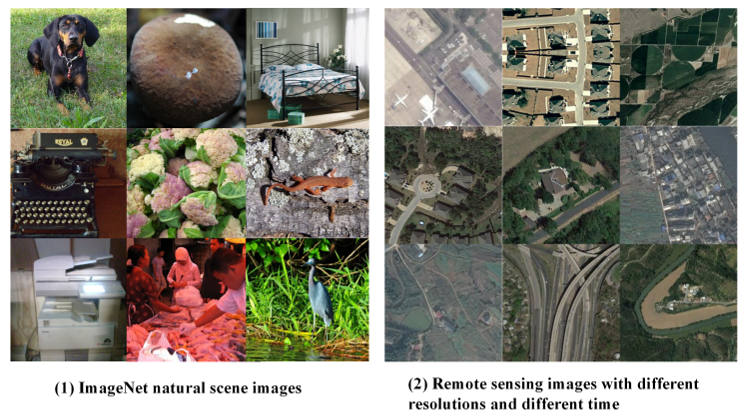
\includegraphics[width=\textwidth]{paper_figures/基于AI基础模型微调的变化检测模型研究/ChangeCLIP/changeclip2.png}
  \caption{ImageNet自然场景图像与遥感图像的比较.}
  \label{fig:changeclip2}
\end{figure}

\begin{figure}[!htbp]
  \centering
  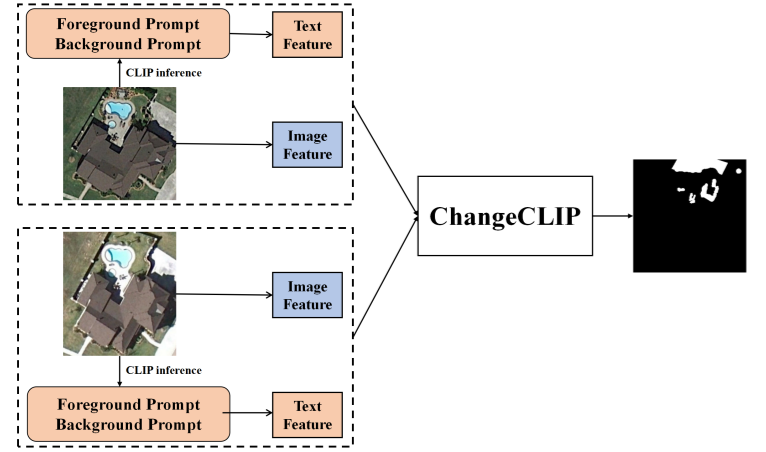
\includegraphics[width=\textwidth]{paper_figures/基于AI基础模型微调的变化检测模型研究/ChangeCLIP/changeclip1.png}
  \caption{多模态遥感变化检测架构.}
  \label{fig:changeclip1}
\end{figure}




本节将CLIP引入RSCD任务,并提出了一个多模态变化检测框架,命名为ChangeCLIP,如图~\ref{fig:changeclip1}所示。在多模态变化检测任务中,通常使用单一模态,主要是遥感影像,来识别变化。为了结合基于文本的提示信息,利用CLIP模型基于56个常见的地表覆盖分类生成描述性提示,如表I所示。这些分类涵盖了遥感数据集中常见的目标元素。本节进一步将这56种类型归类为更广泛的分类,以便参考,如表~\ref{tab:remote_sensing_categories}所示。如图~\ref{fig:changeclip2}的文本框所示,为遥感图像的前景和背景特征设计了特定的提示,利用CLIP模型作为基础。通过这种方式,构建了一个基本数据集,丰富了用于变化检测任务的多模态先验信息。在图像编码阶段,本节构建了一个Siamese神经网络,从双时相遥感影像中提取图像特征。在文本编码阶段,本节应用Transformer网络从文本提示中提取文本特征。为了充分利用多模态特征学习的优势,本节在ChangeCLIP中有效地结合了视觉和文本特征。此外,本节提出了一种新颖的差异特征补偿(Differential Feature Compensation,DFC)模块,用于输出语义变化。


\begin{table}[!htbp]
  \centering
  \caption{遥感影像中的常见地物类别}
  \label{tab:remote_sensing_categories}
  \begin{tabularx}{\linewidth}{@{}l X@{}}
    \toprule
    Category                      & Items \\
    \midrule
    Natural Environment           & Beach, Forest, Lake, Meadow, Mountain, Sea, Wetland, Cotton Field, Farmland, Prairie, Desert, River, Tree, Shrubbery, Chaparral, Fertile Land, Snow Land, Pond, Island \\
    \midrule
    Transportation                & Airport, Bridge, Freeway, Harbor, Railway, Interchange, Intersection, Road, Highway \\
    \midrule
    Recreation \& Sports          & Basketball Court, Ground Track Field, Stadium, Tennis Court, Golf Course \\
    \midrule
    Residential \& Buildings      & Dense Residential, Single-Family Residential, Building, Church, Cabin \\
    \midrule
    Commercial \& Industrial      & Commercial Area, Industrial Area, Oil Tank, Storage Tanks, Container, Mine \\
    \midrule
    Other Man-made Structures     & Terrace, Campus, Park, Parking Lot, Square, Solar Panel, Cars, Ship, Airplane, Runway, Impermeable Surface \\
    \bottomrule
  \end{tabularx}
\end{table}

\subsection{ChangeCLIP网络设计}
\subsubsection{ChangeCLIP总体结构设计}
本节提出了一种创新的方法ChangeCLIP,利用大规模视觉-语言模型来处理遥感变化检测(RSCD)任务。如图~\ref{fig:changeclip3}所示,ChangeCLIP的综合框架分为四个主要部分:多模态数据、多模态编码器、差异特征补偿和视觉-语言驱动解码器。在第一个部分,利用CLIP模型的无监督分类能力为遥感影像生成文本提示,从而构建多模态输入数据,用于变化检测任务。第二部分,采用CLIP模型构建图像和文本编码器,作为多模态RSCD任务的基础双时相特征提取器。此外,将图像特征与文本特征相结合,有效补偿了传统单模态变化检测方法中的局限性。第三部分,为了增强模型捕捉双时相变化的能力,引入了差异特征补偿(DFC)模块。该模块利用多种计算方法表示差异特征,并通过特征图的加权融合,优化了对不同双时相影像差异的适应能力。在最后一个部分,充分利用从编码阶段获得的视觉-语言特征。通过将这些视觉-语言特征与解码阶段的特征相结合,设计了一个视觉-语言驱动的解码器。

\begin{figure}[!htbp]
  \centering
  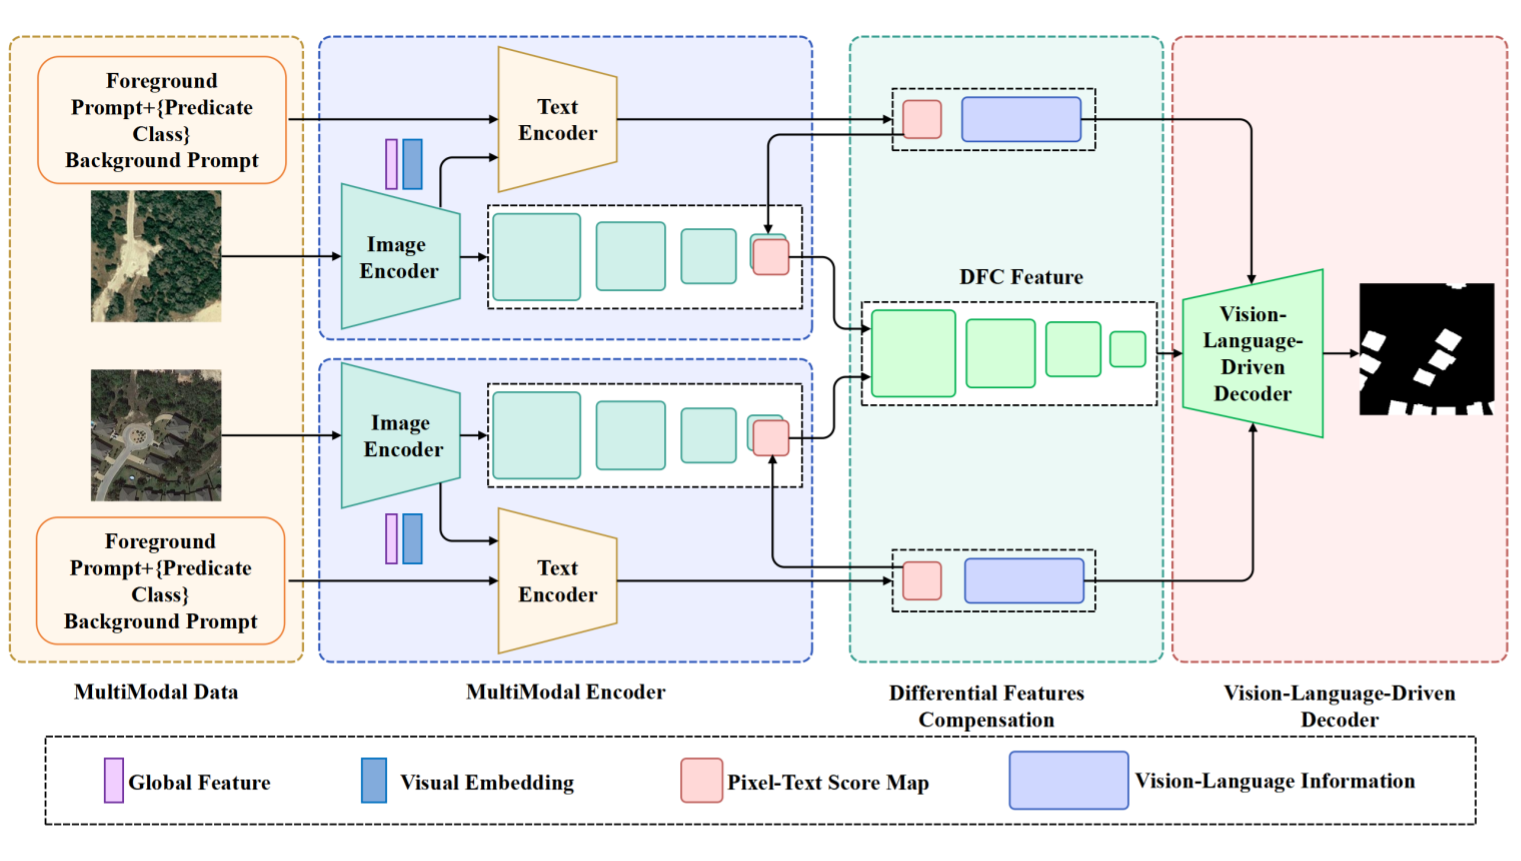
\includegraphics[width=\textwidth]{paper_figures/基于AI基础模型微调的变化检测模型研究/ChangeCLIP/changeclip3.png}
  \caption{ChangeCLIP 变化检测架构。Global Feature (全局特征) 是从图像中获取的、具有物体识别能力的特征信息。Visual Embedding (视觉嵌入) 是高层特征图,被视为图像的嵌入。Pixel-Text Score Map (像素-文本得分图) 是图像与文本提示之间的相关性图。Vision-Language Information (视觉-语言信息) 意味着结合了图像特征和文本特征。}\label{fig:changeclip3}
\end{figure}

\subsubsection{多模态编码器}
如今,计算机视觉和自然语言处理(NLP)越来越紧密地结合在一起,催生了许多将计算机视觉和NLP相结合的优秀项目~\cite{Chen2021VisualGPTDA, Lu2019ViLBERTPT}。在ChangeCLIP模型中,通过将CLIP的大规模图像-文本先验知识与变化检测相结合,提出了一种多模态遥感影像变化检测(RSCD)框架,如图\ref{fig:changeclip3}所示。由于当前没有像素级的变化检测数据集提供文本提示标签,本节利用CLIP的无监督预测能力来制定原始的遥感影像文本提示。具体而言,为了获得双时相影像的文本表示,本节使用CLIP模型对这56个类别进行预测,如表I所示。本节选择了具有最高置信度的9个类作为预测类别。因此,前景的文本描述设置为``遥感影像前景物体,\{预测类别\}'', 而``遥感影像背景物体''作为背景的文本描述。本节的目标是变化区域,因此使用预测类别组成前景的文本提示,正如上述所提到的那样。通过这种方式,变化物体可以通过双时相文本提示直接展示,而双时相文本提示提供了遥感先验知识。最终,ChangeCLIP的输入由两对并行的图像编码器和文本编码器组成。

图像编码器和文本编码器从 CLIP 模型的图像编码器和文本编码器中选取,以有效利用 CLIP 模型强大的图像–文本建模能力。在特征提取阶段,双流图像编码器获得两组特征金字塔$\{F_{a1},F_{a2},F_{a3},F_{a4}\}$ 和 $\{F_{b1},F_{b2},F_{b3},F_{b4}\}$,分别表示双时相的多级特征。在计算机视觉中,深度网络的特征维度较高且具有更强的判别能力,因此通常认为高层次图像特征能够表征图像的语义信息。因此,将高层次语义特征图与文本序列特征相结合。为了结合高层次语义特征图与文本序列特征,ResNet~\cite{He2015DeepRL}主干和 ViT~\cite{Dosovitskiy2020AnII}主干有所区别:在 ResNet 的情况下,使用注意力池化模块生成高层次语义特征,将其视为图像序列特征;而在 ViT 中,则直接将高层次特征作为图像序列特征。这种在 ViT 中的图像序列特征与文本序列特征的对齐有助于促进两种模态之间更紧密的表示。来自 ViT 主干的图像序列特征天然地与文本序列特征对齐,增强了模型捕捉两种模态内在关系和语义一致性的能力。相比 ResNet 主干,ViT 在多模态任务上通常具有更好的表征能力。以 ResNet 为例来描述该部分的计算步骤,因为 ResNet 的序列特征提取算法相较 ViT 更为复杂。视觉编码过程结束时,使用注意力池化模块对高层次特征图进行视觉嵌入,以构建图像序列特征。进一步地,在多模态特征提取阶段有效地结合图像信息和文本信息,共同更新多模态特征提取的权重。计算步骤如下:
\begin{align}
x_1 &= \mathrm{Reshape}(x) \label{eq:changeclip-1}\\
x_{\mathrm{avg}}(i,j) &= \frac{1}{HW}\sum_{h_w=1}^{HW} x(h_w, i, j) \label{eq:changeclip-2}\\
x_2 &= \mathrm{Concat}\bigl(x_{\mathrm{avg}}, x_1\bigr) \label{eq:changeclip-3}\\
x_3 &= x_2 + \mathrm{pos\_embedding} \label{eq:changeclip-4}\\
x_4 &= \mathrm{softmax}\!\Bigl(\frac{x_3 x_3^{\mathrm{T}}}{\sqrt{d_k}}\Bigr)\,x_3 \label{eq:changeclip-5}\\
x_5 &= \mathrm{Reshape}(x_4) \label{eq:changeclip-6}\\
\mathrm{global\_feature} &= x_5[:,:,0] \label{eq:changeclip-7}\\
\mathrm{visual\_embedding} &= \mathrm{Reshape}\bigl(x_5[:,:,1]\bigr) \label{eq:changeclip-8}
\end{align}

其中,$x\in\mathbb{R}^{n\times c\times h\times w}$ 表示 ResNet 在编码阶段提取的高层次特征图,包含了整个图像的高维语义信息;$n,c,h,w$ 分别表示批大小(batch size)、通道数、特征图的高度和宽度。$x_1\in\mathbb{R}^{hw\times nc}$ 将输入特征图从二维重塑为一维序列。$x_{\mathrm{avg}}$ 表示平均池化的结果,代表输入特征图的全局信息。将二维特征图重塑为一维序列会破坏像素间的空间关系,因此使用位置嵌入(pos\_embedding)来补充特征图的位置信息。如公式 \eqref{eq:changeclip-5} 所示,多头注意力模块用于处理带有全局信息的视觉序列特征图,产生 $\mathrm{global\_feature}\in\mathbb{R}^{n\times (c/2)}$ 和 $\mathrm{visual\_embedding}\in\mathbb{R}^{n\times (c/2)\times h\times w}$。$d_k$ 是用于调整注意力模块敏感度的缩放因子。$\mathrm{global\_feature}$ 表示原始输入图像的全局语义类别信息;$\mathrm{visual\_embedding}$ 是经过嵌入编码后的视觉特征图,可与后续的文本序列特征结合。为了适应变化检测双流网络的特性,分别提取双时相图像的特征,然后计算双时相图像的 $\mathrm{global\_feature}$ 和 $\mathrm{visual\_embedding}$。

为了更好地利用文本提示提供的语义信息与图像信息之间的关联,需要将文本编码特征与图像特征结合,以计算文本与图像结合后的特征序列。在 ChangeCLIP 中,图像序列特征由上述提到的 \(\mathrm{global\_feature}\) 和 \(\mathrm{visual\_embedding}\) 组成。从文本编码器获得的文本语义特征通过 Transformer 模块与图像的特征序列相结合。其计算步骤如下:
\begin{align}
t_2 &= F_{\mathrm{te}}(t_1) \label{eq:changeclip-9}\\
\hat t_2 &= F_{\mathrm{cd}}(t_2, V) \label{eq:changeclip-10}\\
t_3 &= t_2 + \gamma \times \hat t_2 \label{eq:changeclip-11}\\
\mathrm{score\_map} &= \eta(t_3)\times \eta(V') \label{eq:changeclip-12}
\end{align}

其中,\(t_1\) 是文本 token;\(F_{\mathrm{te}}\) 是基于 Transformer 的文本编码器;\(t_2\) 是 Transformer 生成的文本嵌入;\(V\) 表示将 \(\mathrm{global\_feature}\) 和 \(\mathrm{visual\_embedding}\) 结合后的特征表示;\(F_{\mathrm{cd}}\) 是图像特征序列与文本嵌入之间进行上下文解码的解码器;通过 \(F_{\mathrm{cd}}\) 的计算,图像特征序列和文本嵌入得以通过上下文解码器中的 Transformer 块有效结合,而 \(\hat t_2\) 是 \(F_{\mathrm{cd}}\) 的输出。在公式 \eqref{eq:changeclip-11} 中,通过可学习系数 \(\gamma\) 将 \(\hat t_2\) 与 \(t_2\) 相结合,以有效关联图像特征与文本特征。于是,包含文本与图像信息的 \(t_3\) 可以表征图像视觉特征与文本语义特征结合后的信息。因此,在解码阶段将 \(t_3\) 作为视觉–语言特征的补充,与解码中的视觉特征 \(V'\) 结合。\(V'\) 是在图像编码阶段从高层次语义特征计算得到的 \(\mathrm{visual\_embedding}\),\(\eta\) 是归一化函数。通过上述计算方法得到逐像素—文本的 \(\mathrm{score\_map}\)。\(\mathrm{score\_map}\) 表示图像视觉嵌入与文本特征序列之间的关系。在本节中,\(\mathrm{score\_map}\) 与图像特征提取中的高层次语义特征结合,以补充高层次语义特征中的文本相关语义信息,使高层次语义特征图更加具有判别力。

\subsubsection{结合余弦相似度计算的混合差异特征计算方法}

传统的变化检测方法通常基于语义分割来进行任务处理。然而,这种方法存在一个缺点,即忽略了任务中最重要的变化特征。变化检测的主要关注点是遥感影像在不同时间段的变化区域,而不是特定的语义类别。通过使用语义分割,重点在于将像素分类为不同的语义类别,这对于遥感影像中的变化检测并不适用。因此,遥感影像变化检测(RSCD)的核心在于模型对变化特征的表示能力。为了解决这个问题,提出了一种新型的差异特征补偿(DFC)模块,该模块基于不同时间段遥感影像的差异特征计算,如图4所示。通过DFC模块,网络可以专注于通过不同的特征计算模块学习双时相遥感影像的变化特征,而不是语义类别。因此,本节提出的方法比依赖语义分割的传统方法更能针对遥感影像的变化检测。

具体来说,双时相遥感影像在空间上表现出一致性,但在地理上存在时间差异。在这一阶段,常见的双时相特征融合策略是使用Concat计算方法。从深度学习的理论基础出发,Concat的计算方法只是将双时相特征图合并,差异特征的体现通过反向传播算法学习。在双时相特征融合中,Concat并没有突出差异特征在RSCD任务中的重要性。因此,我们考虑使用另外两种更直接的差异特征计算方法。对于双时相特征,特征的差异主要体现在两个方面,一方面是像素特征序列的数值差异,如减法。另一方面是基于余弦相似度的像素特征序列在高维空间中的语义差异。对于前者,简单的减法计算方法可以更好地表达高层特征图中的差异。但在低层特征图中,由于不同时间阶段的相同类型地物可能具有较大的颜色差异,减法计算方法很难准确表达变化特征。对于后者,余弦相似度可以有效捕捉高维向量的相似性。在双时相特征分析的背景下,余弦相似度弥补了减法在表示向量方向差异方面的不足。因此,从差异表示的角度来看,减法和余弦相似度是互补的。

基于上述分析,本节设计了用于差异学习的 DFC 模块。首先,通过特征图相减计算差异。由于算法的识别目标是变化区域,单纯的特征图相减结果无法充分表达该区域在语义上的特征。因此,为更好地适配双时相图像变化的特点,对相减结果取绝对值,以更好地表达通过相减获得的兴趣区域显著图,并引入卷积模块,使网络能够自适应地优化相减后的特征图。由此生成的特征图能够突出显示变化区域的特征。与此同时,考虑到余弦距离能够在高维空间中表示不同特征向量的相似性,设计了另一种基于余弦距离的特征差异计算模块。综上,DFC 的计算步骤如下:
\begin{align}
F_{\mathrm{sub}} &= \sigma\bigl(\lvert F_a - F_b\rvert\bigr) \label{eq:changeclip-13}\\
\varphi &= \frac{x_1 \cdot x_2}{\max\bigl(\lVert x_1\rVert_2 \cdot \lVert x_2\rVert_2,\ \varepsilon\bigr)},\quad x_1\in F_a,\ x_2\in F_b,\ \varepsilon=1\times10^{-8} \label{eq:changeclip-14}\\
m &= \varphi\bigl(1 - \varphi(F_a, F_b)\bigr) \label{eq:changeclip-15}\\
X &= \mathrm{FPN}\bigl(\mathrm{concat}(F_a, F_b)\bigr) \label{eq:changeclip-16}\\
\hat X &= \mathrm{CA}\bigl(\mathrm{concat}(X \times m,\ F_{\mathrm{sub}},\ X)\bigr) \label{eq:changeclip-17}
\end{align}

其中,$F_a$、$F_b$ 是融合了不同时相视觉–语言信息的特征图;$\sigma$ 表示卷积模块;$F_{\mathrm{sub}}$ 为特征图相减后取绝对值得到的差异图;$\varphi$ 表示余弦相似度计算;$\varepsilon$ 为防止分母为零的极小常数;$m$ 是通过双时相特征图的余弦相似度图计算得到的差异图。采用 FPN 模型~\cite{lin_feature_2017}来融合多层级信息;$\hat X$ 为不同计算方法生成的差异特征;CA~\cite{Hu2017SqueezeandExcitationN}为通道注意力模块,用于融合上述方法生成的特征。正如上述所示,本节改变了传统变化检测算法的常规做法,深入探索并成功集成了多种变异特征提取方法。特征图相减虽保留了差异特征的基本计算方式,却牺牲了原始特征图的语义信息;而特征图拼接则保留了完整的双时相特征信息,却缺乏差异特征的显式表征,需要在整个网络中进行学习。为此,引入了基于余弦相似度的计算方案,利用余弦相似度刻画双时相特征的差异图。通过结合特征相减、特征融合与相似性特征学习,网络涵盖多种判别性特征学习策略。此外,在此基础上引入注意力机制,以自适应地控制三种差异特征表示的重要性。该注意力机制能够根据变化区域的重要性自动调整差异特征的权重分布,从而增强网络对变化特征的感知能力。

\subsubsection{视觉-语言驱动的变化检测解码器}

在ChangeCLIP 模型,利用了Swin Transformer~\cite{Liu2021SwinTH}模块,在解码阶段建立了全局注意力关系,从而增强了ChangeCLIP的特征表示能力。此外,本节还提出了一种视觉-语言驱动的解码器,通过引入低秩双线性注意力模块,将编码阶段的视觉-语言特征与解码阶段的图像特征结合,从而补充了解码阶段的语义特征。编码阶段的视觉-语言特征学习了来自图像和文本的丰富语义信息。通过将这些语义信息融入解码阶段,模型能够更好地识别变化区域,并提高整体性能。低秩双线性注意力模块的计算步骤如下:
\begin{align}
q &= W_I \cdot I \label{eq:changeclip-18}\\
k &= W_T \cdot T \label{eq:changeclip-19}\\
v &= W_V \cdot T \label{eq:changeclip-20}\\
\mathrm{attn\_scores} &= \mathrm{softmax}\!\Bigl(\frac{q\,k^{\mathrm{T}}}{\sqrt{d_k}}\Bigr) \label{eq:changeclip-21}\\
\mathrm{output} &= \mathrm{attn\_scores}\,\cdot\,v \label{eq:changeclip-22}
\end{align}

其中,\(I\in\mathbb{R}^{n\times l_1\times d}\) 表示编码阶段提取的 DFC 特征图,\(T\in\mathbb{R}^{n\times l_2\times d}\) 表示编码阶段提取的视觉–语言信息。\(W_I, W_T\in\mathbb{R}^{d\times d_k},\ W_V\in\mathbb{R}^{d\times d_v}\) 是将输入特征映射到低维空间的三个线性变换矩阵。该输出融合了图像特征与文本特征之间的关联信息,生成了一种新的表示,用以刻画图像特征与文本特征之间的互依关系和匹配程度。该表示不仅强化了文本特征与图像特征之间的相关性,也增强了 ChangeCLIP 的表示能力。与此同时,双时相图像的类别信息被包含在文本特征中,因此 ChangeCLIP 对双时相图像中的目标变化更加敏感。

\begin{figure}[!htbp]
  \centering
  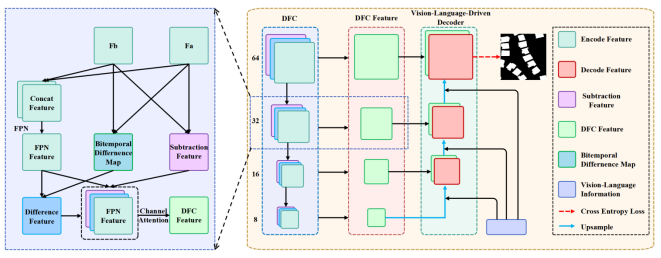
\includegraphics[width=\textwidth]{paper_figures/基于AI基础模型微调的变化检测模型研究/ChangeCLIP/changeclip4.png}
  \caption{ChangeCLIP 的差分特征补偿模块和解码结构。Concat Feature 指的是在编码阶段通过将双时相图像拼接而获得的特征图。Bitemporal Difference Map 指的是通过计算余弦相似度得到的差异图。Subtraction Feature 指的是将双时相图像的特征图相减而得到的特征。}
  \label{fig:changeclip4}
\end{figure}

为了增强 ChangeCLIP 在解码阶段的学习能力,基于 Swin Transformer 块设计了逐层的多级特征融合结构。该结构将高层特征信息传递至低层,并在每个融合级别使用 Swin Transformer 块提升解码表征能力。如图~\ref{fig:changeclip4}所示,详细介绍了 ChangeCLIP 的视觉–语言驱动解码器。在编码阶段,ChangeCLIP 将文本语义信息与图像特征图融合;在解码阶段,对双时相遥感影像的不同特征应用多级特征融合的多模态解码模块,最终获得解码预测结果。其计算步骤如下:
\begin{align}
F_3 &= \mathrm{concat}\bigl(f(D_4,\;\text{text}),\;D_3\bigr)\, \label{eq:changeclip-23}\\
F_2 &= \mathrm{concat}\bigl(f(F_3,\;\text{text}),\;D_2\bigr)\, \label{eq:changeclip-24}\\
F_1 &= \mathrm{concat}\bigl(f(F_2,\;\text{text}),\;D_1\bigr)\, \label{eq:changeclip-25}\\
\mathrm{output} &= \mathrm{Upsample}(F_1)\, \label{eq:changeclip-26}
\end{align}
其中,$D_1, D_2, D_3, D_4$ 是由 DFC 模块生成的不同特征图,$\text{text}$ 是编码阶段提取的双时相视觉–语言特征序列;$f$ 表示 Swin Transformer 块,$\mathrm{output}$ 是通过上采样操作得到的最终预测结果。

总而言之,本节提出了一种强大的视觉-语言驱动解码器,应用于遥感影像变化检测(RSCD)任务中。视觉-语言驱动解码器利用Swin Transformer模块建立全局注意力关系,从而能够在不同层级上对差异特征图进行优化解码,增强了模型在解码阶段的特征表示能力。为了进一步增强解码阶段的表现,引入了一个低秩双线性注意力模块。该模块有效地将编码阶段的视觉-语言特征与解码阶段的视觉特征结合,通过补充解码阶段的语义特征,使得模型能够从遥感影像中提取重要的变化特征,从而实现更精确的变化检测。最后,设计了一个逐层结构来构建解码模块。基于Swin Transformer模块的逐层特征融合结构确保了特征信息从高层到低层的传递,从而保证了在解码阶段能够全面利用重要特征,提升了遥感影像变化检测的性能。总体而言,ChangeCLIP在RSCD任务中利用了视觉-语言驱动的解码器。通过有效地整合视觉和文本信息,实现了对遥感影像变化的更好理解和检测。

\subsection{实验结果与分析}

\begin{figure}[!htbp]
  \centering
  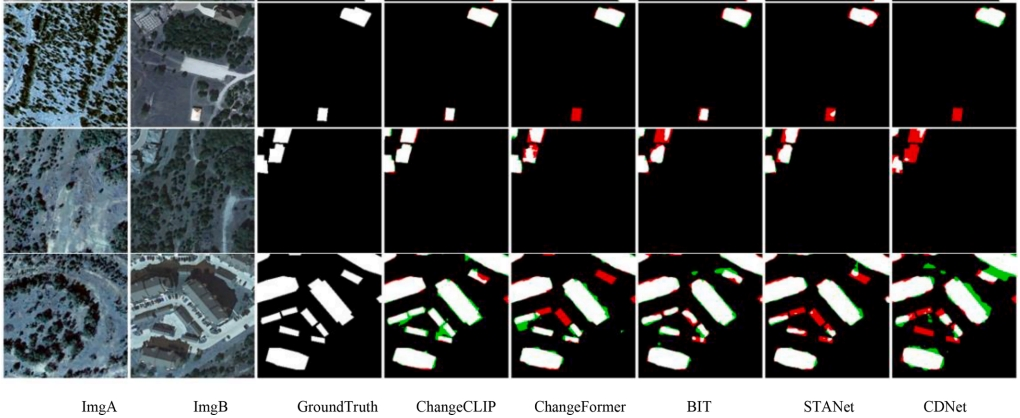
\includegraphics[width=\textwidth]{paper_figures/基于AI基础模型微调的变化检测模型研究/ChangeCLIP/changeclip_levir.png}
  \caption{ChangeCLIP 模型与对比模型在 LEVIR-CD 上的局部可视化对比结果}
  \label{fig:changeclip_levir}
\end{figure}

与之相比,ChangeCLIP首创了一种专门针对遥感变化检测(RSCD)的创新多模态视觉-语言框架,巧妙地融合了视觉和文本数据。通过引入独特的模块,如差异特征补偿(DFC)模块和视觉-语言驱动解码器,进一步创新。这些组件协同作用,增强了变化相关特征的学习和语义理解。多模态输入、差异特征学习和视觉-语言综合的结合使得ChangeCLIP在多个数据集上达到了新的性能基准,取得了最先进的结果。对比分析实验证实了ChangeCLIP在执行RSCD任务时,在CNN、注意力、Transformer、特征融合/差异化和边界感知等多个类别的现有模型中的优越性。

\subsubsection{实验结果量化指标与可视化分析}

如表~\ref{tab:changeclip_levir}、表~\ref{tab:changeclip_levirplus}、表~\ref{tab:changeclip_whucd}、表~\ref{tab:changeclip_cdd}至表~\ref{tab:changeclip_sysu}所示,在五个数据集(LEVIR-CD、LEVIR-CD+、WHUCD、CDD和SYSU-CD)上广泛评估了ChangeCLIP。根据各种评估指标,ChangeCLIP在所有数据集上都达到了最先进的性能。符号``--''表示原始论文中缺失的数据。对于这些情况,重新训练了部分模型,以获得更高的准确性。与其他变化检测方法相比,ChangeCLIP算法在多种评估指标上表现出了优越的性能。由于这些是二分类变化检测任务,前景变化类别的交并比(IoU)作为主要指标。

对实验结果进行仔细分析发现,在LEVIR-CD数据集上,ChangeCLIP在所有指标上超越了最近的经典变化检测算法。特别是,RN50主干网络达到了85.20\%的IoU。在LEVIR-CD+数据集上,ChangeCLIP在所有标准上都领先于其他方法,且优势显著。此外,ViT主干网络的IoU达到了75.63\%,超过了RN50主干网络。在WHUCD数据集上,ViT和RN50主干网络的IoU均超过了90\%。在这三个以建筑物为重点的数据集中,ChangeCLIP在处理密集小物体场景方面展现出了强大的有效性。ChangeCLIP在LEVIR-CD、LEVIR-CD+和WHUCD上的召回率分别为90.67\%、83.90\%和94.02\%,表明其具有较高的真正检测率和较低的假阴性发生率。这表明ChangeCLIP在实际应用中具有显著的实用价值。

\begin{figure}[!htbp]
  \centering
  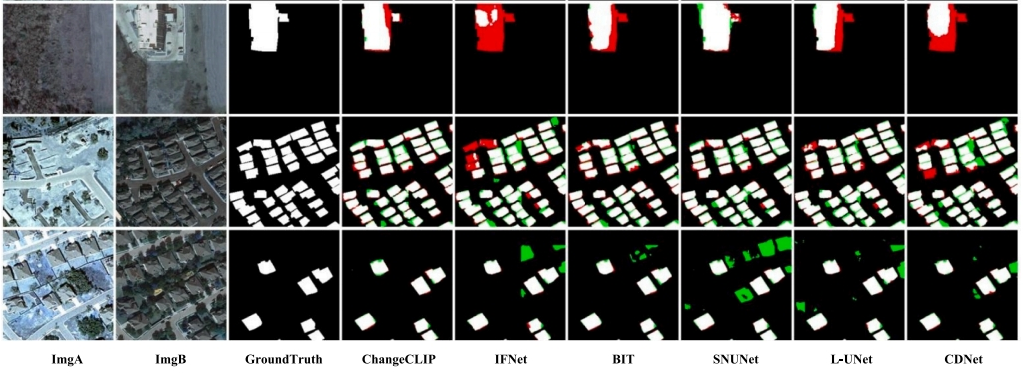
\includegraphics[width=\textwidth]{paper_figures/基于AI基础模型微调的变化检测模型研究/ChangeCLIP/changeclip_levirplus.png}
  \caption{ChangeCLIP 模型与对比模型在 LEVIR-CD+ 上的局部可视化对比结果}
  \label{fig:changeclip_levirplus}
\end{figure}

在CDD数据集上,ChangeCLIP达到了95.87\%的IoU,超过了最近提出的变化检测算法。这一表现展示了ChangeCLIP在检测一般变化区域方面的能力,同时也证明了CDD数据集高质量的标注,使得ChangeCLIP强大的拟合能力得以充分发挥。在SYSU-CD数据集上,ChangeCLIP达到了71.41\%的IoU,同样超越了最新的算法。与CDD类似,SYSU-CD也是为检测一般变化区域而设计的。

在图~\ref{fig:changeclip_levir}、图~\ref{fig:changeclip_levirplus}、图~\ref{fig:changeclip_whucd}、图~\ref{fig:changeclip_cdd}和图~\ref{fig:changeclip_sysu}中,展示了在LEVIR-CD、LEVIR-CD+、WHUCD、CDD和SYSU-CD上的测试结果可视化。选择了ChangeCLIP模型中IoU得分最高的模型,并将其与近年来的经典算法进行比较。在这些可视化结果中,真正阳性(TP)由白色像素表示,真正阴性(TN)由黑色表示,假阳性(FP)由绿色表示,假阴性(FN)由红色表示。可视化结果明确展示了ChangeCLIP在各种数据集和应用场景中都能实现出色的检测性能,与地面真实标注紧密对齐。

\begin{table}[!htbp]
  \centering
  \caption{ChangeCLIP 模型在 LEVIR-CD 数据集上的定量结果}
  \label{tab:changeclip_levir}
  \begin{tabular*}{\textwidth}{@{\extracolsep{\fill}} l c c c c c c c}
    \toprule
    Model & OA & mF1 & mIoU & IoU & F1 & Rec & Prec \\
    \midrule
    CDNet~\cite{Alcantarilla2016StreetviewCD}                         & 98.35 & 91.49 & 85.25 & 72.21 & 83.87 & 84.14 & 83.61 \\
    STANet~\cite{chen_spatial-temporal_2020}                        & 98.92 & 94.22 & 89.54 & 80.20 & 89.02 & 85.80 & 92.49 \\
    BIT~\cite{chen_remote_2022}                           & 98.95 & 93.22 & 89.93 & 80.86 & 89.48 & 87.53 & 90.65 \\
    MFATNet~\cite{Mao2022MFATNetMF}                       & 99.03 & --    & --    & 82.42 & 90.36 & 88.93 & 91.85 \\
    ChangeFormer~\cite{bandara2022transformer}                  & 99.04 & --    & 90.82 & 82.66 & 90.50 & 90.18 & 90.83 \\
    HMCNet~\cite{Wang2022HMCNetHE}                        & 99.07 & --    & --    & 83.05 & 90.74 & 89.82 & 91.68 \\
    AFCF3D-Net~\cite{Ye2023AdjacentLevelFC}                    & --    & --    & --    & 83.08 & 90.76 & 90.17 & 91.35 \\
    LGPNet~\cite{Liu2022BuildingCD}                        & 99.16 & --    & 91.38 & 83.63 & 91.09 & 89.38 & 92.87 \\
    TransUNetCD~\cite{Li2022TransUNetCDAH}                   & --    & --    & --    & 83.67 & 91.11 & 89.82 & 92.43 \\
    FHD~\cite{pei_feature_2022}                           & 99.10 & 95.33 & 91.39 & 83.72 & 91.14 & 90.32 & 91.97 \\
    DMATNet~\cite{Song2022RemoteSI}                       & 98.25 & --    & --    & 84.13 & 90.75 & 89.98 & 91.56 \\
    STransUNet~\cite{Yuan2022STransUNetAS}                    & 99.13 & --    & --    & 84.19 & 91.41 & 90.55 & 92.30 \\
    \textbf{ChangeCLIP (RN50)}    & \textbf{99.20} & \textbf{95.79} & \textbf{92.18} & \textbf{85.20} & \textbf{92.01} & \textbf{90.67} & \textbf{93.40} \\
    ChangeCLIP (ViT-B/16)         & 99.14 & 95.42 & 91.54 & 83.99 & 91.30 & 89.04 & 93.68 \\
    \bottomrule
  \end{tabular*}
\end{table}

\begin{table}[!htbp]
  \centering
  \caption{ChangeCLIP 模型在 LEVIR-CD+ 数据集上的定量结果}
  \label{tab:changeclip_levirplus}
  \begin{tabular*}{\textwidth}{@{\extracolsep{\fill}} l c c c c c}
    \toprule
    Model & OA & IoU & F1 & Rec & Prec \\
    \midrule
    FC-Siam-Di~\cite{Daudt2018FullyCS}               & 98.14 & 61.37 & 76.06 & 72.55 & 79.94 \\
    CDNet~\cite{Alcantarilla2016StreetviewCD}                    & 98.01 & 61.58 & 76.22 & 78.45 & 74.12 \\
    FresUNet~\cite{Daudt2018MultitaskLF}                 & 98.28 & 65.24 & 78.96 & 79.30 & 78.62 \\
    L-UNet~\cite{Papadomanolaki2021ADM}                   & 98.36 & 67.19 & 80.38 & 82.25 & 78.59 \\
    SNUNet~\cite{Fang2021SNUNetCDAD}                   & 98.42 & 68.17 & 80.82 & 79.43 & 80.52 \\
    DTCDSCN~\cite{Liu2019BuildingCD}                  & 98.58 & 68.76 & 81.19 & 79.08 & 83.41 \\
    BIT~\cite{chen_remote_2022}                      & 98.49 & 69.07 & 81.71 & 82.84 & 80.61 \\
    DSIFN~\cite{Zhang2020ADS}                    & 98.61 & 70.97 & 82.29 & 80.32 & 83.77 \\
    ICIF-Net~\cite{Feng2022ICIFNetIC}                 & 98.73 & 71.89 & 83.65 & 80.88 & 87.79 \\
    ChangeCLIP (RN50)        & 98.79 & 73.61 & 84.80 & 82.69 & 87.02 \\
    \textbf{ChangeCLIP (ViT-B/16)} & \textbf{98.90} & \textbf{75.63} & \textbf{86.12} & \textbf{83.90} & \textbf{88.46} \\
    \bottomrule
  \end{tabular*}
\end{table}

\begin{table}[!htb]
  \centering
  \caption{ChangeCLIP 模型在 WHUCD 数据集上的定量结果}
  \label{tab:changeclip_whucd}
  \begin{tabular}{@{}lccccccc@{}}
    \toprule
    Model                      & OA    & mF1   & mIoU  & IoU   & F1    & Rec   & Prec   \\
    \midrule
    DPCCNet~\cite{Papadomanolaki2021ADM}                    & 98.27 & 90.42 & 83.67 & 69.13 & 81.75 & 83.77 & 79.83  \\
    SNUNet~\cite{Fang2021SNUNetCDAD}                     & 98.22 & 90.92 & 84.38 & 70.61 & 82.77 & 92.31 & 75.03  \\
    BIT~\cite{chen_remote_2022}                        & 98.62 & 90.50 & 86.78 & 75.00 & 85.71 & 89.74 & 82.04  \\
    DARNet~\cite{li_densely_2022}                     & 98.75 & 93.14 & 87.79 & 76.89 & 86.93 & 89.85 & 84.20  \\
    ICIFNet~\cite{Feng2022ICIFNetIC}                    & 99.01 & 94.32 & 89.70 & 80.43 & 89.16 & 87.58 & 90.79  \\
    DSIFN~\cite{Zhang2020ADS}                      & 99.14 & 94.94 & 90.74 & 82.37 & 90.33 & 87.13 & 93.78  \\
    P2V~\cite{lin_transition_2023}                        & 99.32 & 96.08 & 92.68 & 86.07 & 92.52 & 90.91 & 94.18  \\
    ChangeCLIP (RN50)          & 99.52 & 97.29 & 94.83 & 90.15 & 94.82 & 94.02 & 95.63  \\
    ChangeCLIP (ViT-B/16)      & 99.52 & 97.27 & 94.79 & 90.08 & 94.78 & 93.58 & 96.02  \\
    \bottomrule
  \end{tabular}
\end{table}

\begin{table}[!htb]
  \centering
  \caption{ChangeCLIP 模型在 CDD 数据集上的定量结果}
  \label{tab:changeclip_cdd}
  \begin{tabular*}{\textwidth}{@{\extracolsep{\fill}} l c c c c c c c}
    \toprule
    Model & OA & mF1 & mIoU & IoU & F1 & Rec & Prec \\
    \midrule
    DSAMNet~\cite{shi_deeply_2022}                 & --    & --    & --    & 88.13 & 93.69 & 92.77 & 94.54 \\
    BESNet~\cite{Lei2022BoundaryEC}                  & 98.51 & --    & 93.30 & 88.28 & 93.77 & 92.39 & 95.20 \\
    SwinSUNet~\cite{zhang_swinsunet_2022}               & 98.50 & --    & --    & --    & 94.00 & 92.30 & 95.70 \\
    ISNet~\cite{Cheng2022ISNetTI}                   & 98.78 & 97.06 & 94.37 & 90.12 & 94.80 & 94.43 & 95.18 \\
    D-TNet~\cite{wan_d-tnet_2022-3}                  & 98.90 & --    & --    & 91.18 & 95.39 & 96.75 & 94.06 \\
    JFSDNet~\cite{Zhou2022JointFD}                 & 99.07 & --    & --    & --    & 95.55 & 92.60 & \textbf{98.75} \\
    IRA-MRSNet~\cite{Ling2022IRAMRSNetAN}              & 99.14 & --    & --    & --    & 96.47 & 96.13 & 96.81 \\
    RCDT~\cite{Lu2022RCDTRR}                    & --    & --    & --    & 93.79 & 96.80 & 96.97 & 96.63 \\
    SSANet~\cite{Jiang2022JointVL}                  & --    & --    & --    & 95.20 & 94.33 & 96.06 & \textbf{99.07} \\
    \textbf{ChangeCLIP (RN50)}    & \textbf{99.48} & \textbf{98.80} & \textbf{97.64} & \textbf{95.87} & \textbf{97.89} & 97.77 & 98.02 \\
    ChangeCLIP (ViT-B/16)   & 99.47 & 98.77 & 97.59 & 95.78 & 97.85 & \textbf{97.81} & 97.88 \\
    \bottomrule
  \end{tabular*}
\end{table}

\begin{table}[!htb]
  \centering
  \caption{ChangeCLIP 模型在SYSU-CD数据集上的定量结果}
  \label{tab:changeclip_sysu}
  \begin{tabular*}{\textwidth}{@{\extracolsep{\fill}} l c c c c c c c}
    \toprule
    Model & OA & mF1 & mIoU & IoU & F1 & Rec & Prec \\
    \midrule
    DSAMNet~\cite{shi_deeply_2022}                   & --    & --    & --    & 64.18 & 78.18 & \textbf{81.86} & 74.81 \\
    CDNet~\cite{Alcantarilla2016StreetviewCD}                     & 89.90 & 85.86 & 75.99 & 64.34 & 78.30 & 77.29 & 79.34 \\
    ISNet~\cite{Cheng2022ISNetTI}                     & 90.01 & --    & --    & 64.44 & 78.29 & 80.27 & 76.41 \\
    SNUNet~\cite{Fang2021SNUNetCDAD}                    & 90.79 & 86.80 & 77.41 & 66.02 & 79.54 & 75.87 & 83.58 \\
    L-UNet~\cite{Papadomanolaki2021ADM}                    & 90.58 & 86.75 & 77.30 & 66.15 & 79.63 & 78.08 & 81.24 \\
    DSIFN~\cite{Zhang2020ADS}                       & 90.74 & 87.06 & 77.75 & 66.90 & 80.17 & 79.37 & 80.98 \\
    DPCC-Net~\cite{Papadomanolaki2021ADM}                  & --    & --    & --    & 66.63 & 79.97 & 78.93 & 81.05 \\
    DARNet~\cite{li_densely_2022}                    & 91.26 & --    & --    & 68.10 & 81.03 & 79.11 & 83.04 \\
    ICIFNet~\cite{Feng2022ICIFNetIC}                   & 91.24 & --    & --    & 68.12 & 80.74 & 78.51 & 83.37 \\
    SSANet~\cite{Jiang2022JointVL}                    & --    & --    & --    & 68.18 & 81.08 & 79.73 & 82.48 \\
    ChangeCLIP (RN50)         & 92.08 & 88.79 & 80.38 & 70.53 & 82.72 & 80.41 & 85.16 \\
    AFCF3D-Net~\cite{Ye2023AdjacentLevelFC}                & --    & --    & --    & 71.09 & 83.11 & \textbf{83.88} & 82.30 \\
    \textbf{ChangeCLIP (ViT-B/16)} & \textbf{92.46} & \textbf{89.23} & \textbf{81.06} & \textbf{71.41} & \textbf{83.32} & 79.80 & \textbf{87.16} \\
    \bottomrule
  \end{tabular*}
\end{table}

\begin{figure}[!htbp]
  \centering
  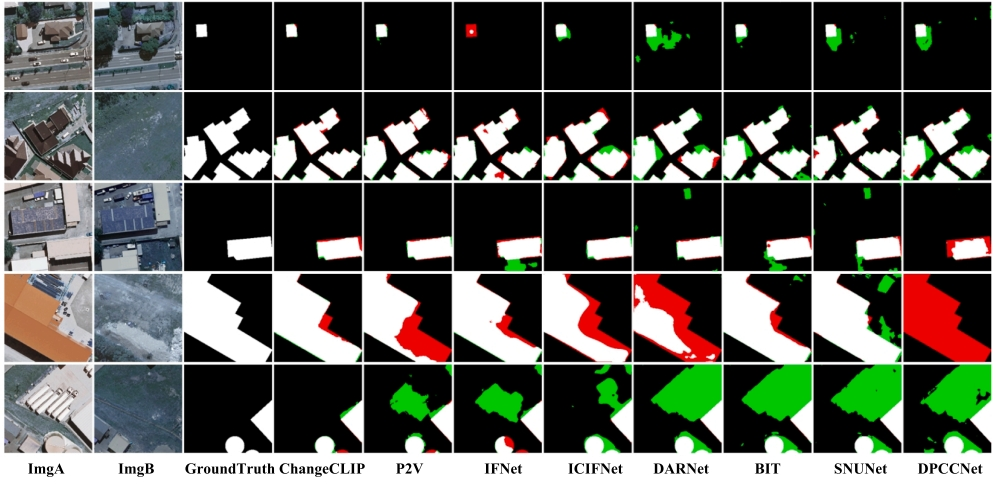
\includegraphics[width=\textwidth]{paper_figures/基于AI基础模型微调的变化检测模型研究/ChangeCLIP/changeclip_whucd.png}
  \caption{ChangeCLIP 模型与对比模型在WHUCD数据集上的可视化对比结果}
  \label{fig:changeclip_whucd}
\end{figure}

% \begin{comment}

\subsubsection{ChangeCLIP消融实验}

如表~\ref{tab:changeclip_ablation_resnet}和表~\ref{tab:changeclip_ablation_vit}所示,进行了广泛的消融实验,以验证ChangeCLIP中关键组件的贡献,包括多模态编码器(ME)、差异特征补偿(DFC)模块和视觉-语言驱动解码器(VLDD)。由于变化检测任务中前景类和背景类的比例差异很大,表VIII使用前景类的IoU指数作为比较的基础。基线模型仅使用CLIP的主干网络作为图像编码器,并使用基础的FPN结构进行双时相特征融合。基线模型中的解码器是FCN。该单模态模型提供了性能基准。逐步添加ME、DFC和VLDD模块在各数据集上持续提高准确性,证明了每个创新的价值。ME指的是使用图像和文本信息的多模态编码器,DFC表示加入差异特征补偿模块,VLDD表示视觉-语言驱动解码器。

在消融实验的三个实验中比较了变化检测任务中常用的差异特征计算模块,包括Concat、减法和DFC模块。该部分的消融实验结果表明,直接使用减法进行差异特征计算的表现不如使用Concat进行双时相特征融合。这与前文的分析一致。与Concat相比,DFC模块通过结合不同方面的差异特征,具有更强的差异特征表示能力。

\begin{figure}[!htbp]
  \centering
  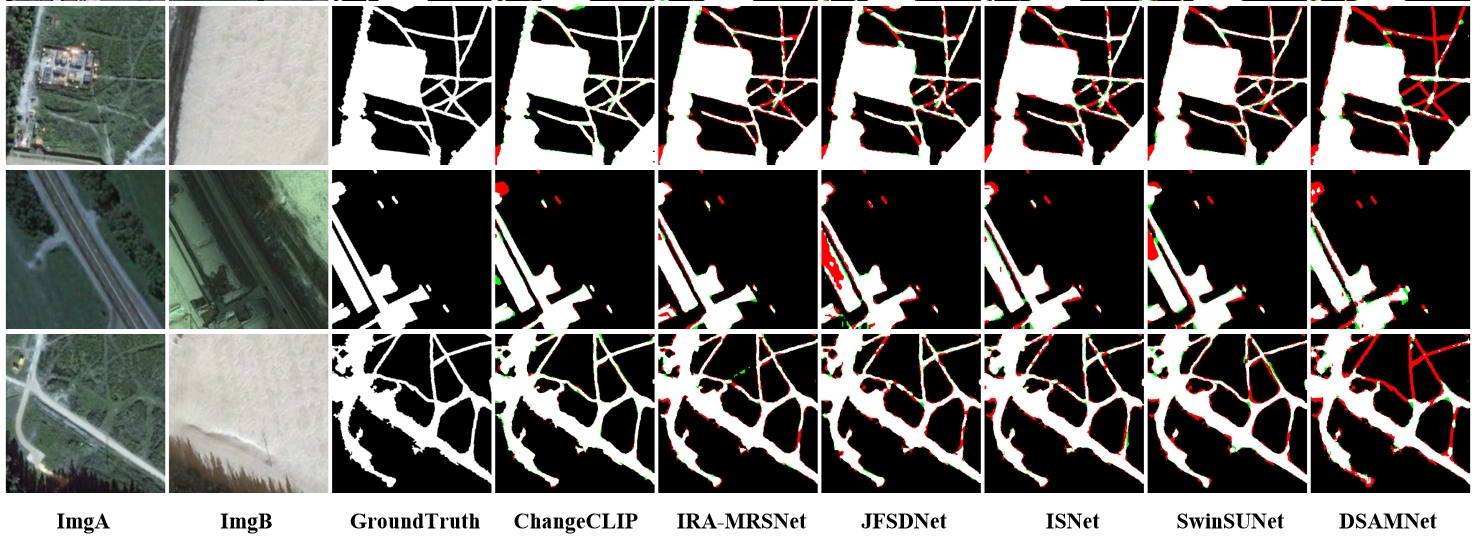
\includegraphics[width=\textwidth]{paper_figures/基于AI基础模型微调的变化检测模型研究/ChangeCLIP/changeclip_cdd.png}
  \caption{ChangeCLIP 模型与对比模型在 CDD 上的可视化对比结果}
  \label{fig:changeclip_cdd}
\end{figure}

\begin{figure}[!htbp]
  \centering
  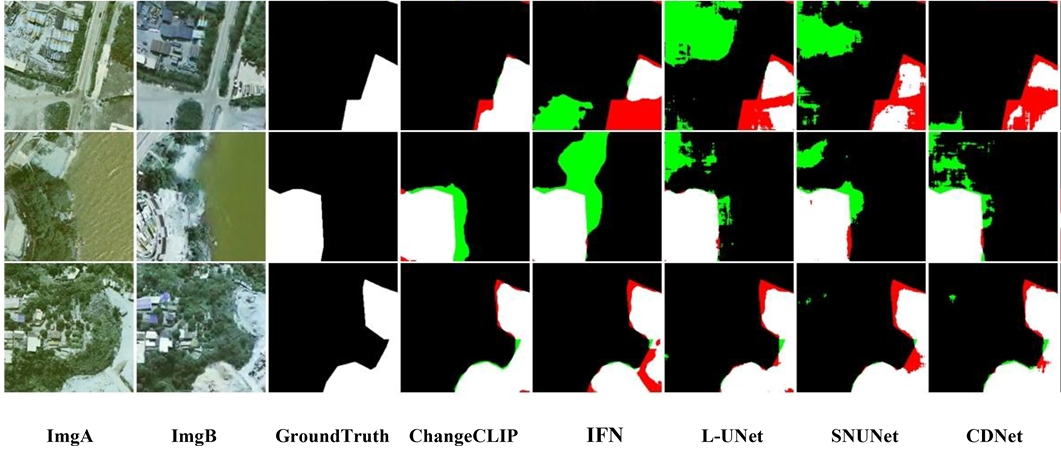
\includegraphics[width=\textwidth]{paper_figures/基于AI基础模型微调的变化检测模型研究/ChangeCLIP/changeclip_sysu.png}
  \caption{ChangeCLIP 模型与对比模型在 SYSU-CD 上的可视化对比结果}
  \label{fig:changeclip_sysu}
\end{figure}

\begin{figure}[!htbp]
  \centering
  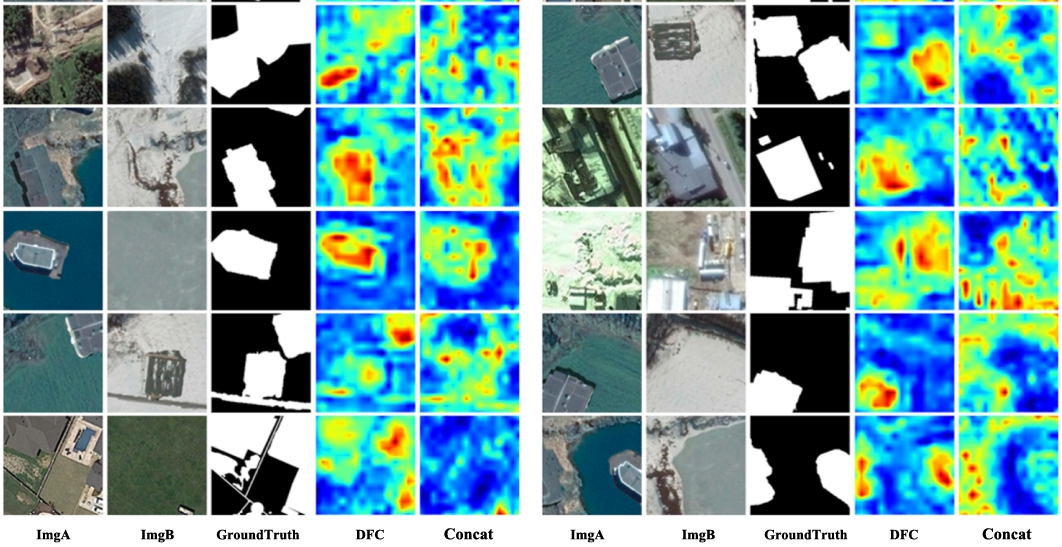
\includegraphics[width=\textwidth]{paper_figures/基于AI基础模型微调的变化检测模型研究/ChangeCLIP/changeclip_hotmap.png}
  \caption{不同的差异特征方法与 ChangeCLIP 的特征热图在 CDD 数据集上的可视化对比结果}
  \label{fig:changeclip_hotmap}
\end{figure}

具体来说,通过ME集成文本语义与基于视觉的基线相比,性能有所提升,突出了多模态的优势。显然,通过多模态信息补充图像信息,有助于增强模型对遥感图像中语义特征的理解。由于VLDD需要包括来自ME组件的视觉-语言信息,无法仅对Baseline+VLDD进行消融研究。因此,将Baseline+ME和Baseline+ME+VLDD的实验结果进行了比较。可以看出,VLDD在解码器中结合了文本和视觉表示,带来了额外的提升。

\begin{table}[!htb]
\centering
\small
\setlength{\tabcolsep}{2pt} % 紧凑列距
\caption{基于 RN50 骨干的 IoU 消融实验。Base:仅用图像编码器;ME:多模态编码器;I:Image Encoder;T:Text Encoder;DFC:差异特征补偿;VLDD:视觉-语言驱动解码器;FPN:特征金字塔;FCN:全卷积;Sub:减法。}
\label{tab:changeclip_ablation_resnet}
\begin{tabular}{@{}l c c c *{5}{c}@{}}
\toprule
\textbf{Model} & \textbf{Encoder} & \textbf{Neck} & \textbf{Decoder} &
\makecell{\textbf{LEVIR-}\\\textbf{CD}} &
\makecell{\textbf{LEVIR-}\\\textbf{CD+}} &
\textbf{CDD} &
\makecell{\textbf{SYSU-}\\\textbf{CD}} &
\textbf{WHU} \\
\midrule
Base            & I     & FPN       & FCN  & 75.25 & 68.61 & 89.74 & 61.71 & 87.56 \\
Base(Sub)       & I     & FPN(Sub)  & FCN  & 71.19 & 60.98 & 86.37 & 44.13 & 80.88 \\
Base+DFC        & I     & FPN+DFC   & FCN  & 75.85 & 70.46 & 89.86 & 69.34 & 89.01 \\
Base+ME         & I\&T  & FPN       & FCN  & 76.01 & 70.51 & 89.91 & 65.64 & 87.74 \\
Base+ME+VLDD    & I\&T  & FPN       & VLDD & 84.72 & 72.62 & 95.72 & 68.68 & 89.59 \\
ChangeCLIP      & I\&T  & FPN+DFC   & VLDD & 85.20 & 73.61 & 95.87 & 70.53 & 90.15 \\
\bottomrule
\end{tabular}
\end{table}


\begin{table}[!htb]
\centering
\small
\setlength{\tabcolsep}{2pt}
\caption{基于 ViT-B/16 骨干的 IoU 消融实验。记号同表 \ref{tab:changeclip_ablation_resnet}。}
\label{tab:changeclip_ablation_vit}
\begin{tabular}{@{}l c c c *{5}{c}@{}}
\toprule
\textbf{Model} & \textbf{Encoder} & \textbf{Neck} & \textbf{Decoder} &
\makecell{\textbf{LEVIR-}\\\textbf{CD}} &
\makecell{\textbf{LEVIR-}\\\textbf{CD+}} &
\textbf{CDD} &
\makecell{\textbf{SYSU-}\\\textbf{CD}} &
\textbf{WHU} \\
\midrule
Base            & I     & FPN       & FCN  & 74.73 & 68.16 & 88.77 & 64.82 & 79.22 \\
Base(Sub)       & I     & FPN(Sub)  & FCN  & 74.31 & 68.75 & 83.67 & 64.45 & 79.73 \\
Base+DFC        & I     & FPN+DFC   & FCN  & 75.24 & 68.59 & 90.25 & 68.42 & 82.53 \\
Base+ME         & I\&T  & FPN       & FCN  & 75.35 & 69.12 & 90.54 & 65.64 & 82.83 \\
Base+ME+VLDD    & I\&T  & FPN       & VLDD & 83.41 & 71.73 & 94.13 & 69.76 & 82.81 \\
ChangeCLIP      & I\&T  & FPN+DFC   & VLDD & 83.99 & 75.63 & 95.78 & 71.41 & 90.08 \\
\bottomrule
\end{tabular}
\end{table}




有趣的是,DFC本身的表现几乎与ME相同,这表明在ChangeCLIP中,变化特征建模和多模态信息对变化检测任务的影响是相等的。将减法作为双时相图像融合方法在FPN之前的效果比Concat更差。这可能是因为直接使用特征减法会丢失大部分双时相图像的信息,使得网络难以学习变化的表示。包含所有组件的完整ChangeCLIP模型达到了最佳结果,每个模块提供了互补的优势。总之,广泛消融分析定量展示了ChangeCLIP中提出的多模态编码器、差异特征补偿模块和视觉-语言驱动解码器的独特贡献。通过与消融版本和基线模型的准确性提升,验证了ChangeCLIP 模型中的创新。

\begin{table}[!htb]
  \centering
  \caption{ChangeCLIP模型在RSCD数据集上基于ResNet-50和ViT-B/16骨干模型的结果}
  \label{tab:changeclip_backbone}
  \begin{tabular*}{\textwidth}{@{\extracolsep{\fill}} l l c c c c c c c}
    \toprule
    Dataset       & Backbone     & OA    & mF1   & mIoU  & IoU   & F1    & Rec   & Prec  \\
    \midrule
    \multirow{2}{*}{WHUCD}
                  & RN50         & 99.52 & 97.29 & 94.83 & 90.15 & 94.82 & 94.02 & 95.63 \\
                  & ViT-B/16     & 99.52 & 97.27 & 94.79 & 90.08 & 94.78 & 93.58 & 96.02 \\
    \midrule
    \multirow{2}{*}{CDD}
                  & RN50         & 99.48 & 98.80 & 97.64 & 95.87 & 97.89 & 97.77 & 98.02 \\
                  & ViT-B/16     & 99.47 & 98.77 & 97.59 & 95.78 & 97.85 & 97.81 & 97.88 \\
    \midrule
    \multirow{2}{*}{SYSU-CD}
                  & RN50         & 92.08 & 88.79 & 80.38 & 70.53 & 82.72 & 80.41 & 85.16 \\
                  & ViT-B/16     & 92.46 & 89.23 & 81.06 & 71.41 & 83.32 & 79.80 & 87.16 \\
    \midrule
    \multirow{2}{*}{LEVIR-CD}
                  & RN50         & 99.20 & 95.79 & 92.18 & 85.20 & 92.01 & 90.67 & 93.40 \\
                  & ViT-B/16     & 99.14 & 95.42 & 91.54 & 83.99 & 91.30 & 89.04 & 93.68 \\
    \midrule
    \multirow{2}{*}{LEVIR-CD+}
                  & RN50         & 98.79 & 92.08 & 86.18 & 73.61 & 84.80 & 82.69 & 87.02 \\
                  & ViT-B/16     & 98.90 & 92.77 & 87.24 & 75.63 & 86.12 & 83.90 & 88.46 \\
    \bottomrule
  \end{tabular*}
\end{table}



\subsubsection{ChangeCLIP在不同的骨架网络的结果}

根据本节的实验,对CLIP模型中的两个骨干网络,RN50(ResNet50)和ViT(ViT-B/16),进行了详细比较。根据表表~\ref{tab:changeclip_backbone}中的结果,在使用的5个代表性数据集上,ViT骨干网络在SYSU-CD和LEVIR-CD+数据集上的表现远优于RN50骨干网络,在CDD和WHUCD数据集上接近RN50,在LEVIR-CD数据集上的表现则较差。可以看出,ViT和RN50在不同数据集上的表现有所不同,但总体上它们都表现出了较高的准确性。ViT的整体表现略优于RN50。这可以归因于几个因素。首先,ViT相比RN50模型具有更广泛的全局感受野。这意味着ViT能够更好地捕捉遥感影像中目标个体之间的全局关联信息。其次,在RN50骨干网络中,使用了一个注意力池化模块来生成高层语义特征,这些特征被用来替代图像序列特征。而在ViT框架中,直接将高层特征作为图像序列特征。与RN50骨干网络相比,ViT骨干网络生成的图像序列特征与文本序列特征更加一致,这使得ViT骨干网络在多模态任务中表现得更好。

\subsubsection{ChangeCLIP中差异特征图热图可视化分析}

可视化热图为ChangeCLIP在遥感影像变化检测(RSCD)任务中感知变化特征的能力提供了宝贵的见解。观察可得,使用ChangeCLIP能够生成具有更强判别性的特征图,这表明其对遥感影像中变化区域的敏感度增强。与传统的特征图热图通常突出前景中的显著区域不同,变化检测的主要目标是识别变化区域。在图~\ref{fig:changeclip_hotmap}中,展示了ChangeCLIP在CDD数据集上的特征图可视化。具体而言,``DFC''表示通过DFC模块处理后的融合特征图的编码部分特征,而``Concat''表示双时相影像在图像特征提取后得到的融合特征图。从图中可以看出,与DFC模块之前的特征图相比,经过DFC模块处理后的特征图在变化特征上展现了更好的效果。特征热图展示了ChangeCLIP在双时相遥感影像中对变化区域的强烈感知能力,突显了本节提出的方法在变化检测任务中的优越性。

\subsection{ChangeCLIP模型的可行性分析与未来工作展望}

\subsubsection{基于多模态视觉-语言表示学习的变化检测}

在本节中,结合了CLIP的无监督推理能力,为遥感影像构建了基本的文本提示。然而,类别语义信息通常在遥感影像语义分割中更为重要,因为在变化检测中,目标是感知变化区域,而不是区分特定的类别。因此,在变化检测任务中指定文本提示需要更好地契合变化检测的任务需求。因此,背景类别很难为变化检测任务制定合适的文本提示。根据提出的消融实验,显然,结合文本的多模态变化检测在多个数据集上始终能达到卓越的算法精度。可以明确看出,多模态信息的融合确实为推动遥感影像变化检测(RSCD)在不同数据集上的进展做出了贡献。同时,在提出的方法的解码阶段,引入了一种新机制,进一步增强了变化检测的性能。通过引入低秩双线性注意力模块,促进了来自解码阶段的图像特征与编码阶段的视觉-语言特征的融合。这种集成使得模型能够有效捕捉视觉和文本模态之间的互补信息,从而提升特征表示和增强RSCD性能。低秩双线性注意力机制促进了解码特征与编码的视觉-语言特征的对齐和交互,增强了模型捕捉遥感影像语义上下文的能力。这种创新的融合方法加强了模型对RSCD任务的理解,并提高了其在遥感影像变化识别中的判别能力。然而,针对解码阶段的视觉-语言结合,可以探索一种更合适的方式,将编码阶段的视觉-语言特征与解码阶段的视觉特征进行结合。

\subsubsection{image-score map的应用}

在本节提出的ChangeCLIP中,基于文本提示和图像视觉信息计算了图像-文本得分图。对于图像-文本得分图的应用,将得分图与视觉编码阶段的高层语义特征图进行拼接,并直接利用文本信息来补充语义信息。依据在语义分割任务中广泛应用的多层次特征融合理论,得分图可以与高层语义特征图及浅层特征图进行结合,以在浅层网络阶段补充文本的语义信息。然而,在实际的网络设计中,生成多层次的得分图需要大量的计算。因此,在结合得分图与视觉编码阶段的过程中,仍有很大的改进空间,可以构思出一个合适的模块来更好地将得分图与视觉编码阶段结合。

\subsubsection{差异特征计算}

在标准变化检测模型中,依赖语义分割任务是常见的做法。然而,在变化检测任务中,重点应该是提取和学习目标区域的变化特征。基于常用的差异特征计算方法,设计了一个差异特征补偿(DFC)模块。DFC模块整合了几种常用的差异特征构建方法,使网络能够以自适应的方式有效学习来自不同差异特征构建方法的差异特征。通过增强变化检测网络学习变化特征的能力,DFC模块有效提升了ChangeCLIP的性能。

在不同数据集上的实验结果揭示了提高变化检测准确性的两种主要方式。首先,像Transformer这样的强大特征提取器可以增强网络对遥感影像的表示能力。其次,像特征融合和差异化这样的技术可以帮助网络更好地捕捉变化特征。在LEVIR-CD+和CDD等数据集上的结果显著提高了网络的性能,其中ChangeCLIP利用Transformer和DFC模块取得了最先进的结果。因此,未来应该更多关注变化相关特征的学习,使得网络更符合变化的识别,从而提高变化检测算法的效果。

\subsection{小结}

在本节中,提出了一种名为ChangeCLIP的多模态框架,用于通过利用多模态视觉-语言信息在遥感影像中进行变化检测。通过整合遥感影像的文本语义信息,增强了视觉模型感知遥感变化的能力。提出的差异特征补偿模块整合了常用的差异特征计算方法,优化了变化检测中差异特征融合的方式。此外,还提出了一种名为视觉-语言驱动解码器的多模态变化检测解码方法,旨在补充解码阶段的语义信息。在解码阶段融合文本和视觉特征,使得ChangeCLIP能够生成更准确和全面的表示,提升变化检测任务的性能。为了评估ChangeCLIP的有效性,在5个基准变化检测数据集(LEVIR-CD、LEVIR-CD+、WHUCD、CDD和SYSU-CD)上进行了全面的实验。实验结果表明,提出的ChangeCLIP模型显著优于现有的最先进方法,在所有5个数据集上达到了前所未有的性能。此外,本节还对ChangeCLIP进行了系统分析,揭示了其潜在的机制,并为未来可能的改进提供了见解。展望未来,多模态范式将在遥感图像处理领域获得越来越多的关注。通过开发更有效的变化检测语言提示,ChangeCLIP的性能有着巨大的提升空间,同时,ChangeCLIP也将成为多模态遥感影像变化检测(RSCD)的基准。这些合适的提示可以更好地引导模型学习与变化相关的特征,进而进一步提高变化检测性能。


\section{基于视觉基础模型微调的变化检测方法}

\subsection{视觉基础模型与变化检测任务概述}

遥感影像变化检测(Remote Sensing Change Detection, RSCD)是遥感领域的重要研究方向,其目标是通过对比多时相遥感影像来识别地表的变化区域。在实际应用中,RSCD 面临多重挑战。首先,遥感数据具有多时相性、多源多样性和多尺度变化等特征。其次,现有高分辨率遥感数据集往往规模有限,标注成本高昂,且缺乏充足的大规模预训练样本。此外,由于异构传感器和成像条件变化所导致的域偏移问题,严重阻碍了现有模型的跨域泛化能力。这些问题在复杂场景下会导致变化检测模型性能的下降。

近年来,深度学习的快速发展不断推动着变化检测方法的演进。从早期的卷积神经网络(CNNs)到视觉 Transformer,再到近期的通用视觉基础模型(Vision Foundation Models, VFMs),模型的特征提取与泛化能力逐步增强。VFMs 如 SAM~\cite{Kirillov2023SegmentA}、DINO~\cite{Caron2021EmergingPI,simeoni2025dinov3} 和 CLIP~\cite{Radford2021LearningTV},通常在大规模图像语料上进行预训练,展现出强大的零样本与迁移学习能力。然而,这些模型的预训练数据主要来自自然场景图像,而遥感影像则多为垂直俯视视角拍摄,具有复杂的目标组合和大尺度空间结构。这一显著的分布差异在将 VFMs 直接应用于遥感变化检测时,造成了性能瓶颈。

为应对上述挑战,一方面需要充分利用 VFMs 的表征优势,另一方面需要采用针对遥感任务的有效适配策略。尽管全参数微调能够带来较强的任务适应性,但其计算与存储开销巨大,限制了在资源受限场景中的部署。因此,近年来参数高效微调(Parameter-Efficient Fine-Tuning, PEFT)方法逐渐受到关注。通过冻结大部分预训练参数,仅更新少量新增模块,PEFT 在显著降低训练成本的同时,能够实现高效的任务适应并保持性能。

\begin{figure}[!htbp]
  \centering
  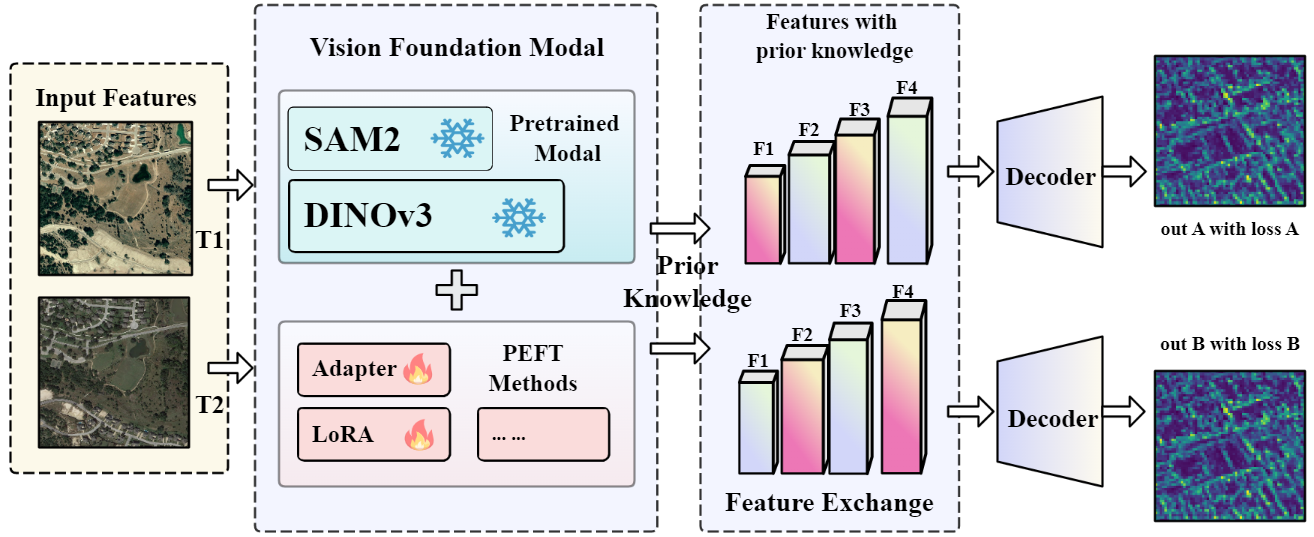
\includegraphics[width=\textwidth]{paper_figures/基于AI基础模型微调的变化检测模型研究/PeftCD/peftcd_framework.png}
  \caption{PeftCD 架构示意图。双时相影像通过注入 PEFT 模块的共享视觉基础模型编码器进行特征提取,特征在解码前进行交换,最终生成变化检测图。}
  \label{fig:peftcd_framework}
\end{figure}

基于上述动机,本节提出了一种基于 VFM 微调的全新变化检测框架——\textbf{PeftCD(Parameter-Efficient Fine-Tuning Change Detection)}。如图~\ref{fig:peftcd_framework}所示,我们选取了两类具有代表性的 VFMs 作为骨干:具备强大分割先验的 \textbf{Segment Anything Model v2 (SAM2)},以及自监督表征学习模型 \textbf{DINOv3}。在此基础上,我们引入了两种典型的 PEFT 方法:\textbf{LoRA}~\cite{LORA} 与 \textbf{Adapter}~\cite{adapter},以实现对遥感场景的高效适配。值得注意的是,除适配外,我们进一步观察到,ViT 类骨干(如 DINOv3)在经过 patch embedding 之后会以固定分辨率进行特征表示,缺乏类似 FPN 的多尺度金字塔结构,这在直接应用于像素级 RSCD 时容易导致边界模糊与伪变化敏感性。为释放其潜力,我们设计了 \textbf{多层融合与上下文增强(Multi-layer Fusion and Context Enhancement, MFCE)解码器},其结构如图~\ref{fig:peftcd_dino3cd} 所示。MFCE 在同尺度下实现跨 Transformer 层的深度注意力融合,并通过 ASPP 风格的上下文模块增强感受野。MFCE 解码器在不引入复杂解码头的前提下,有效补充了 DINOv3 的语义表征能力。而在另一实例中,SAM2 的实现(SAM2CD;见图~\ref{fig:peftcd_sam2cd})则结合了 FPN 与轻量级 ResBlock 解码器,更好地利用其分割先验。

\subsection{视觉基础模型简介}

\subsubsection{分割基础模型:SAM2}
Segment Anything Model 2 (SAM2)~\cite{ravi2024sam} 是原始 SAM~\cite{Kirillov2023SegmentA} 的一次重大升级,旨在提供更高质量且更高效的交互式与自动化图像分割。SAM2 在包含超过 11 亿分割掩膜的 SA-1B 数据集上进行训练,从而学习到丰富的目标结构、边界以及层次关系。与传统的分割模型不同,SAM2 的核心在于其可提示分割(promptable segmentation)能力,即模型能够根据点、边界框、掩膜或文本等多种提示,对图像中的任意目标进行分割。即使在缺少提示的情况下,模型也能自动生成场景中所有目标的分割结果。

在变化检测任务中,分割的本质是对目标边界进行精确刻画,以识别新增、消失或形态发生变化的对象。得益于大规模训练,SAM2 在边界捕获方面展现出卓越的能力,这与变化检测的核心需求高度契合。尤其是在建筑物、道路或水体的细粒度变化场景中,SAM2 可作为强有力的先验知识来源,提供高质量的目标级空间线索,从而提升整体的分割精度。

\subsubsection{自监督表征学习模型:DINOv3}
DINOv3~\cite{simeoni2025dinov3} 代表了自监督视觉 Transformer 的最新进展,标志着大规模无标签数据学习的前沿。不同于依赖人工标注的监督学习,自监督学习直接从数据本身中提取监督信号(如预测图像的被遮挡 patch),迫使模型在无标签条件下学习更加本质且鲁棒的表征。DINOv3 借鉴了 iBOT~\cite{Zhou2021iBOTIB} 等先进范式,并在高达 170 亿张无标签图像上进行训练,从而获得了可广泛迁移至多样化视觉任务的通用语义特征。

这些特征不仅具备强大的语义判别能力,同时对光照、视角或颜色变化的敏感性较低,更稳定地反映了目标的结构与语义属性。在遥感影像变化检测任务中,这种鲁棒性尤为关键。季节变换、光照差异与气候波动往往会引入大量伪变化,而传统基于特征的模型容易将其误判为真实变化。相比之下,DINOv3 通过自监督学习得到的表征能够有效抑制由外观变化引起的干扰,从而更准确地区分真实的地物覆盖变化与环境噪声,为变化检测提供稳定可靠的特征支持。


\subsection{参数高效微调方法}

为了有效地将基础模型适配于遥感变化检测任务,本节引入了两种具有代表性的参数高效微调(Parameter-Efficient Fine-Tuning, PEFT)方法:低秩适配(LoRA)~\cite{LORA} 和 Adapter~\cite{adapter}。

\subsubsection{低秩适配(LoRA)}

LoRA~\cite{LORA} 假设下游任务适配所需的权重更新可以通过低秩分解进行良好近似。设原始投影权重为 $\mat{W}_0\in\mathbb{R}^{d\times k}$。通过冻结 $\mat{W}_0$,引入一个低秩增量:
\begin{equation}
\Delta \mat{W}=\frac{\alpha}{r}\,\mat{B}\mat{A},\qquad
\mat{A}\in\mathbb{R}^{r\times k},\;\mat{B}\in\mathbb{R}^{d\times r},\;r\ll\min(d,k)
\end{equation}
从而得到更新后的权重:
\begin{equation}
\widehat{\mat{W}}=\mat{W}_0+\Delta \mat{W}
\end{equation}
前向传播可表示为:
\begin{equation}
\vect{h}=\widehat{\mat{W}}\,\vect{x}
=\mat{W}_0\vect{x}+\frac{\alpha}{r}\,\mat{B}\mat{A}\,\vect{x}
\end{equation}
在训练过程中,仅有 $\mat{A}$ 和 $\mat{B}$(以及可选的缩放超参数 $\alpha$)会被更新,而 $\mat{W}_0$ 保持冻结不变。在本节中,LoRA 模块被注入到 Transformer 的多头自注意力(Multi-Head Self-Attention, MHSA)中的特定线性投影部分。其超参数设置为 $r{=}8$,$\alpha{=}32$。LoRA 的优势在于其简洁高效,仅引入少量额外参数,却能够有效引导模型朝向任务相关的表征。

\subsubsection{Adapter}

Adapter~\cite{adapter} 是最早提出的 PEFT 方法之一。其核心思想是在每个 Transformer 块内部,以与主干网络并行的方式插入一个轻量级的“瓶颈”结构。典型的 Adapter 模块由一个降维全连接层、一个非线性激活函数(如 GELU),以及一个升维全连接层构成。在前向传播中,输入特征首先通过降维投影进行压缩,再经过非线性激活,最后通过升维投影恢复维度,并通过残差连接与原始特征相加。Adapter 的灵活性在于其插入位置的多样性,可以在特定层增强任务适应性,因此特别适合定制化微调。其计算过程可表示为:
\begin{equation}
    h_{\text{Adapter}}(x) = W_{\text{up}} f(W_{\text{down}} x) + x,
    \label{eq:adapter}
\end{equation}
其中 $x$ 表示 Transformer 块的输出,$f$ 为非线性激活函数。在微调过程中,仅有 Adapter 模块的内部权重 $W_{\text{down}}$ 与 $W_{\text{up}}$ 会被更新。Adapter 的优势在于其结构灵活且模块化,能够方便地集成至任意层的现有模型中。


\begin{table}[!htbp]
\centering
\caption{PeftCD 所用的 PEFT 配置。LoRA 设置 \textbf{dropout}=0.1,注入于 \texttt{qkv} 投影层。所有编码器权重均被冻结,仅 PEFT 模块可训练。Adapter 在每个编码器块前插入残差 MLP 结构。}
\label{tab:peftcd_cfg}
\begin{tabular}{l l l c c}
\toprule
\textbf{Backbone} & \textbf{Strategy} & \textbf{Injected Layers} & \textbf{Rank/Dim} & \textbf{Scale $\alpha$} \\
\midrule
SAM2   & LoRA    & MHSA (\texttt{qkv})    & r=8   & 32 \\
SAM2   & Adapter & Pre-block    & dim=32 & -- \\
DINOv3 & LoRA    & MHSA (\texttt{qkv})     & r=8   & 32 \\
DINOv3 & Adapter & Pre-block     & dim=32 & -- \\
\bottomrule
\end{tabular}
\end{table}

\begin{figure}[!htbp]
  \centering
  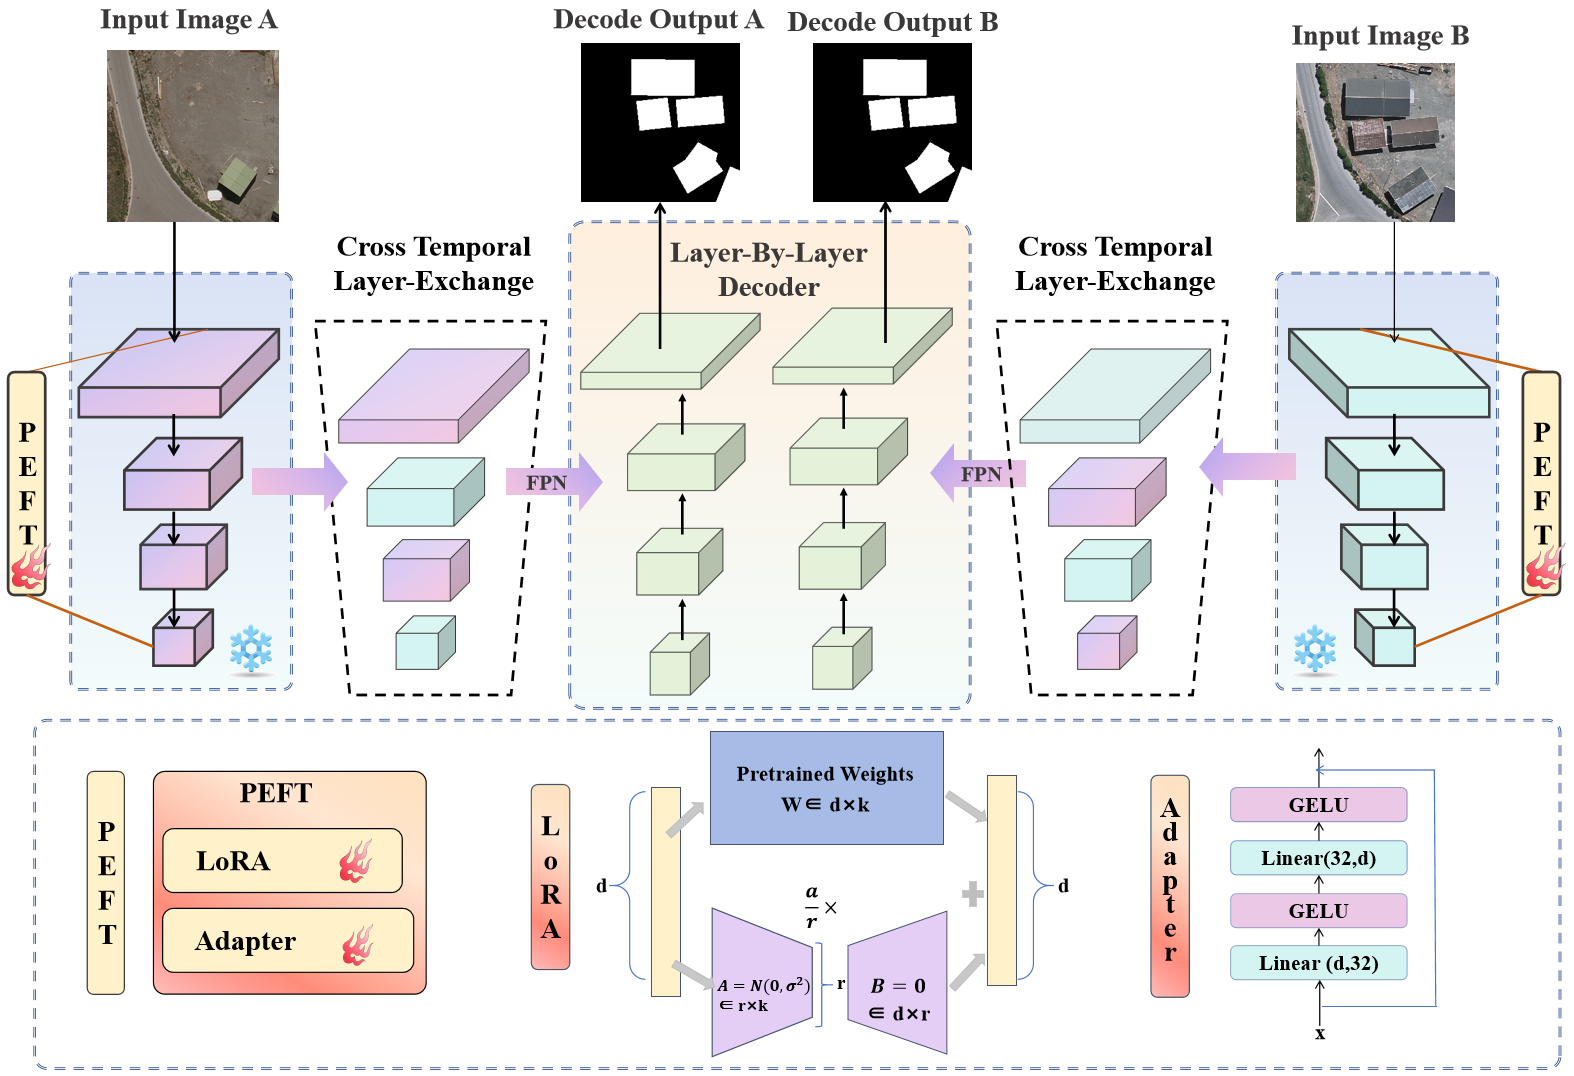
\includegraphics[width=\textwidth]{paper_figures/基于AI基础模型微调的变化检测模型研究/PeftCD/peftcd_sam2cd.png}
  \caption{基于 SAM2 的 PeftCD 模型架构示意图(SAM2CD)。双时相影像输入共享的、插入了PEFT模块的SAM2编码器。提取的特征金字塔经过特征交换后,送入共享的解码器,最终生成变化图。}
  \label{fig:peftcd_sam2cd}
\end{figure}


\subsection{PeftCD模型架构}

\subsubsection{整体思路}

所提出的 PeftCD 框架如图~\ref{fig:peftcd_framework} 所示,基础的变化检测范式采用前文提及的SEED架构。对于一对双时相遥感影像 $X_t$ 和 $X_{t'}$,首先通过共享权重的骨干网络(可选 SAM2 或 DINOv3)提取特征表示。在实验中,我们采用 \texttt{sam2\_hiera\_large} 与 \texttt{dinov3\_vitl16} 作为骨干网络。  
\textbf{参数高效适配}的具体配置如表~\ref{tab:peftcd_cfg} 所示:(i) LoRA被注入至每一个Transformer 块的多头自注意力(MHSA)\texttt{qkv} 投影中,设置秩 $r{=}8$、缩放系数 $\alpha{=}32$、dropout 为 $0.1$;(ii) Adapter则对 每一个编码器块进行封装,采用前置残差 MLP 结构(两层瓶颈结构,激活函数为 GELU,瓶颈维度为 $32$)。在两种策略下,所有骨干网络的参数保持冻结,仅有 PEFT 模块可训练。在编码之后,我们在双时相特征流之间引入特征层交换操作,以促进模型学习与变化相关的表征。交换后的特征再通过一个刻意设计的轻量化解码头进行解码,从而凸显 VFM 骨干网络的表征能力。在基于 SAM2 的架构中,我们采用 FPN 融合特征金字塔,并结合基于 ResBlock 的渐进式上采样解码器生成预测图。而在基于 DINOv3 的架构中,由于其输出为单尺度的高维语义特征,我们设计了解码器,先进行同尺度的多层特征融合与上下文增强(ASPP),再逐步上采样至原始分辨率。

\subsubsection{双时相特征处理与变化检测范式}
在特征交互和解码阶段,PeftCD框架采纳了本文在第六章中提出的SEED(Siamese-Encoder-Exchange-Decoder)范式。我们认为,这种摒弃了显式差异计算的架构,能够最大程度地保留基础模型提取的原始特征信息,充分发挥其强大的表征能力。
\begin{itemize}
    \item \textbf{孪生编码器 (Siamese Encoder):} 双时相影像 $X_t$ 和 $X_{t'}$ 分别通过同一个PEFT微调后的VFM编码器,生成两组多尺度特征金字塔 $\{F_t^i\}_{i=1}^L$ 和 $\{F_{t'}^i\}_{i=1}^L$。权重共享确保了对两幅影像的特征提取具有一致性。
    \item \textbf{特征交换 (Feature Exchange):} 在进入解码器之前,两组特征金字塔进行特征层交换(Layer-Exchange)。例如,奇数层的特征保持不变,偶数层的特征进行交换,从而生成两组混合了双时相信息的特征金字塔。
    \item \textbf{孪生解码器 (Siamese Decoder):} 两组混合特征金字塔分别输入到共享权重的孪生解码器中。解码器通过跳跃连接融合来自编码器的浅层空间信息,并逐层上采样恢复分辨率。最终,两个解码器分支都输出一个变化概率图。在训练时,两个输出都受到同一真实变化标签的监督。
\end{itemize}
在该范式下,模型被训练来识别由特征交换所引入的“时空特征不一致性”,这种不一致性在变化区域表现得尤为剧烈,从而使模型能够隐式地学习到变化的概念。

\begin{figure}[!htb]
  \centering
  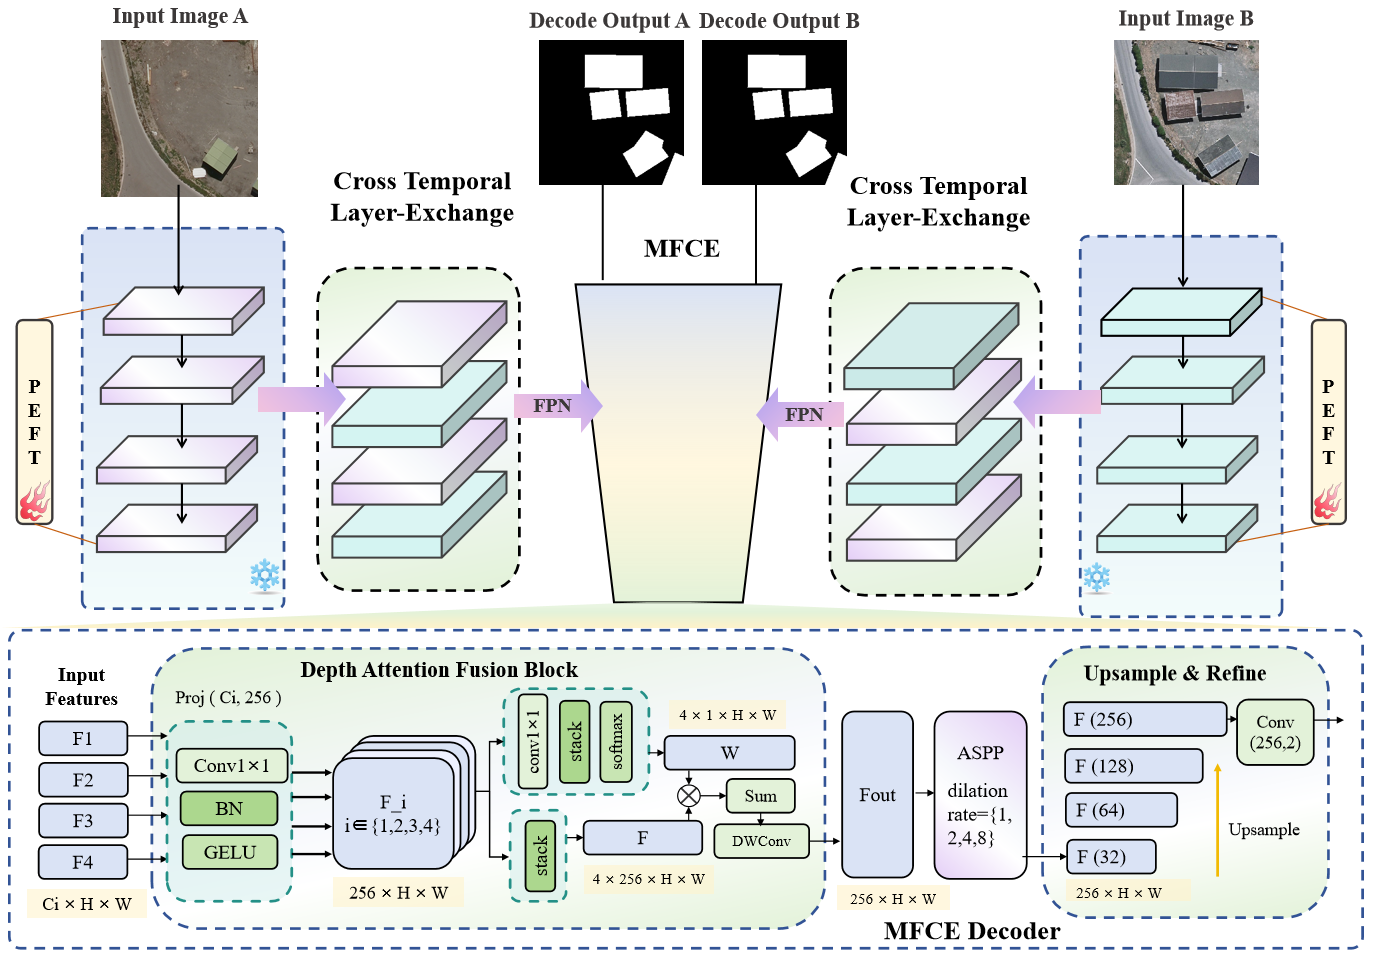
\includegraphics[width=\textwidth]{paper_figures/基于AI基础模型微调的变化检测模型研究/PeftCD/peftcd_dino3cd.png} % 请确保图片路径正确
  \caption{基于DINOv3的PeftCD模型架构(DINO3CD)。该模型采用与SAM2CD类似的SEED范式,但其核心编码器替换为DINOv3,旨在利用其强大的自监督表征来提升对伪变化的鲁棒性。}
  \label{fig:peftcd_dino3cd}
\end{figure}

\subsubsection{基于 SAM2 的 PeftCD架构}

为了将SAM2强大的分割先验知识有效迁移至遥感变化检测任务,我们设计了如图~\ref{fig:peftcd_sam2cd}所示的SAM2CD模型架构。该架构是PeftCD框架的一个具体实现,其核心在于将参数高效微调(PEFT)技术与本文提出的SEED变化检测范式深度融合。

\paragraph{孪生编码器与PEFT注入}
该模型采用孪生编码器(Siamese Encoder)结构来处理双时相输入 $T_1$ 与 $T_2$。其编码器骨干为共享权重的 SAM2 图像编码器,构建于 Vision Transformer (ViT) 之上,能够捕获图像的全局上下文信息。为了在不改变其大规模预训练参数的前提下,将 SAM2 适配于变化检测任务,我们在每个 Transformer 块中注入 PEFT 模块(LoRA 或 Adapter)。具体而言,在每个 Transformer 块中,我们将 LoRA 添加到 MHSA 的 \texttt{qkv} 投影中,参数设置为 $(r{=}8,\ \alpha{=}32,\ \text{dropout}{=}0.1)$;或者,替代性地,用一个前置残差 Adapter MLP(瓶颈维度为 $32$,激活函数为 GELU)对该块进行封装。所有原始的 SAM2 参数保持冻结,仅更新 LoRA/Adapter 的参数。这样的设计既保留了 SAM2 的强边界感知先验,又能高效地引导表征朝向双时相变化特征。  

编码器在每个时相生成一组多尺度特征金字塔。该设计既能保留 SAM2 的通用分割能力,又能高效学习针对双时相遥感影像的判别性特征,从而为后续的变化识别奠定基础。最终,编码器输出两组多尺度特征金字塔,分别以层次化的方式表征对应时相图像,从低层纹理到高层语义。  


\begin{table}[!htb]
\centering
\caption{PeftCD 与经典变化检测模型在 SYSU-CD 数据集上的定量对比结果}
\label{tab:peftcd_sysu}
\begin{tabular}{l c c c c c}
\toprule
\textbf{Model} & \textbf{OA} & \textbf{IoU} & \textbf{F1} & \textbf{Rec} & \textbf{Prec} \\
\midrule
STANet~\cite{chen_spatial-temporal_2020} & 88.24 & 57.22 & 72.79 & 66.71 & 80.08 \\
DSAMNet~\cite{shi_deeply_2022} & -- & 64.18 & 78.18 & 81.86 & 74.81 \\
BIT~\cite{chen_remote_2022} & 90.64 & 66.03 & 79.54 & 77.13 & 82.10 \\
P2V~\cite{lin_transition_2023} & 90.49 & 66.29 & 79.73 & 79.29 & 80.17 \\
HATNet~\cite{Xu2024HybridAT} & 90.92 & 67.00 & 80.24 & 78.23 & 82.36 \\
DARNet~\cite{li_densely_2022} & 91.26 & 68.10 & 81.03 & 79.11 & 83.04 \\
SSANet~\cite{Jiang2022JointVL} & -- & 68.18 & 81.08 & 79.73 & 82.48 \\
CDNeXt~\cite{wei_robust_2024} & 91.99 & 68.57 & 81.36 & 74.10 & 90.20 \\
BASNet~\cite{z_wang_bitemporal_2024} & 91.80 & 69.71 & 82.15 & 80.01 & 84.41 \\
ChangeCLIP~\cite{dong2024changeclip} & 92.08 & 70.53 & 82.72 & 80.41 & 85.16 \\
AGFormer~\cite{Chen2025AGFormerAA} & 92.04 & 70.91 & 82.98 & 82.26 & 83.71 \\
SGSLN~\cite{zhao_exchanging_2023} & -- & 71.05 & 83.07 & 81.45 & 84.76 \\
ChangeMamba~\cite{chen2024changemamba} & 92.30 & 71.10 & 83.11 & 80.31 & 86.11 \\
DEDANet~\cite{Li2025DifferenceEA} & 92.01 & 71.12 & 83.12 & 83.45 & 82.79 \\
DMFANet~\cite{Zhan2025DifferenceAwareMF} & 92.33 & 71.27 & 83.23 & 80.72 & 85.90 \\
UA-BCD~\cite{li_overcoming_2025} & -- & 71.38 & 83.30 & 79.66 & 87.28 \\
DgFA~\cite{f_zhou_dual-granularity_2025}   & 92.42 & 71.86 & 83.63 & 82.08 & 85.24 \\
FTA-Net~\cite{t_zhu_fta-net_2025}   & -- & 72.54 & 84.08 & 82.33 & 85.91 \\
CWmamba~\cite{Liu2025CWmambaLC} & 92.96 & 72.90 & 84.33 & 80.27 & 88.82 \\
SAM-Mamba~\cite{Li2025SAMMambaATC}  & -- & 73.09 & 84.45 & 83.79 & 85.12 \\
DepthCD~\cite{Zhou2025DepthCDDP}   & -- & 73.33 & 84.61 & 83.83 & 85.41 \\
CD-STMamba~\cite{Liu2025CDSTMambaTR} & 93.01 & 73.45 & 84.70 & 82.04 & 87.53 \\
\midrule
PeftCD(DINOv3)  & 93.25 & 73.81 & 84.93 & 80.71 & 89.61 \\
\bottomrule
\end{tabular}
\end{table}

\begin{figure}[!htb]
  \centering
  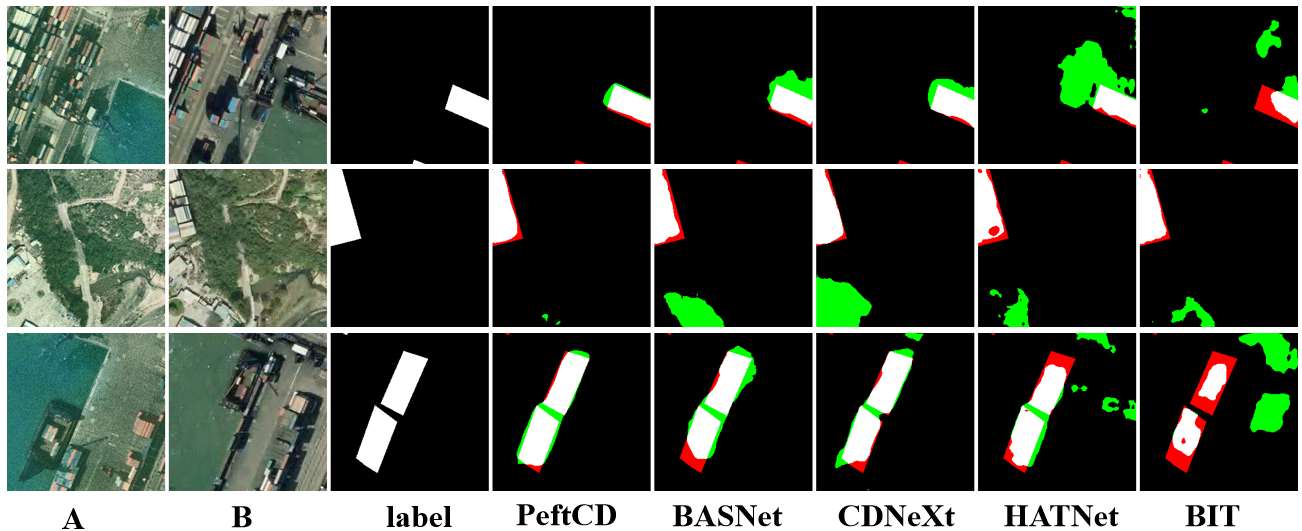
\includegraphics[width=\textwidth]{paper_figures/基于AI基础模型微调的变化检测模型研究/PeftCD/peftcd_sysu.png}
  \caption{PeftCD 模型与对比模型在 SYSU-CD 数据集上的可视化对比结果}
  \label{fig:peftcd_sysu}
\end{figure}


\begin{table}[!htb]
\centering
\caption{PeftCD 与经典变化检测模型在 WHUCD 数据集上的定量对比结果}
\label{tab:peftcd_whucd}
\begin{tabular}{l c c c c c}
\toprule
\textbf{Model} & \textbf{OA} & \textbf{IoU} & \textbf{F1} & \textbf{Rec} & \textbf{Prec} \\
\midrule
P2V~\cite{lin_transition_2023} & 99.31 & 85.91 & 92.42 & 90.93 & 93.97 \\
DSIFN~\cite{Zhang2020ADS} & 99.34 & 86.36 & 92.68 & 90.20 & 95.30 \\
MSCANet~\cite{m_liu_cnn-transformer_2022} & 99.36 & 86.65 & 92.85 & 89.98 & 95.90 \\
SGSLN~\cite{zhao_exchanging_2023} & 99.38 & 87.47 & 93.32 & 92.91 & 93.72 \\
BIT~\cite{chen_remote_2022} & 99.43 & 88.22 & 93.74 & 92.00 & 95.56 \\
HCGMNet~\cite{Han2023HCGMNetAH} & 99.52 & 90.10 & 94.79 & 95.31 & 94.27 \\
ChangeCLIP~\cite{dong2024changeclip} & 99.52 & 90.15 & 94.82 & 94.02 & 95.63 \\
CDNeXt~\cite{wei_robust_2024} & 99.54 & 90.35 & 94.93 & 92.56 & 97.43 \\
CGNet~\cite{han_change_2023} & 99.54 & 90.41 & 94.96 & 94.61 & 95.32 \\
EfficientCD~\cite{dong_efficientcd_2024} & 99.55 & 90.71 & 95.13 & 94.19 & 96.08 \\
SAFDNet~\cite{Fu2025BeyondCD} & 99.55 & 90.73 & 95.14 & 94.47 & 95.82 \\
\midrule
PeftCD & 99.62 & 92.05 & 95.86 & 94.95 & 96.79 \\
\bottomrule
\end{tabular}
\end{table}

\begin{figure}[!htb]
  \centering
  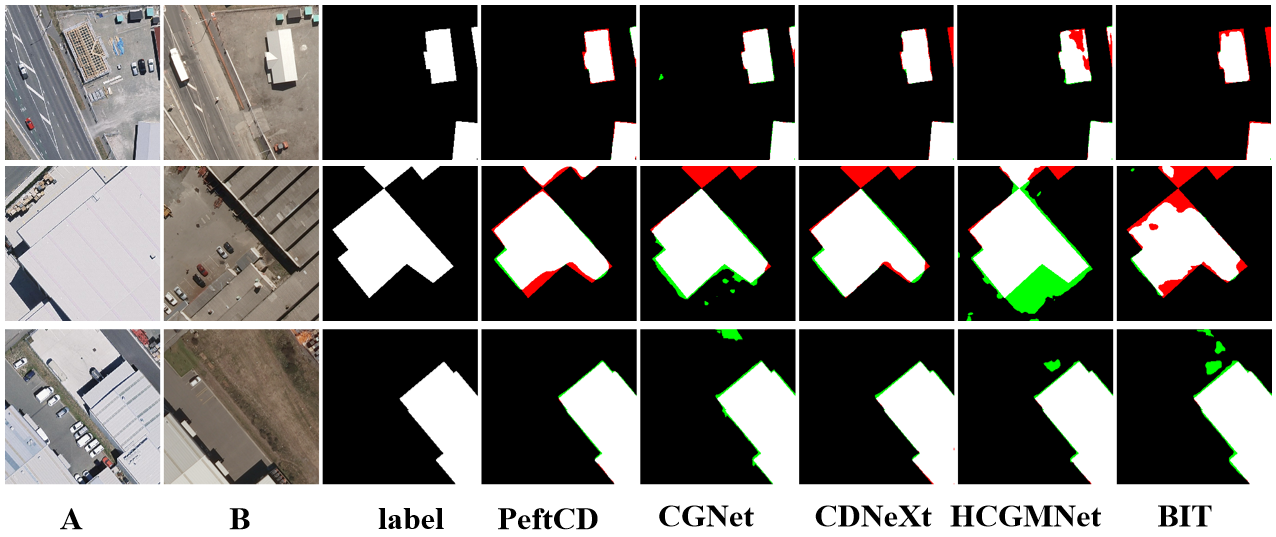
\includegraphics[width=\textwidth]{paper_figures/基于AI基础模型微调的变化检测模型研究/PeftCD/peftcd_whucd.png}
  \caption{PeftCD 模型与对比模型在 WHUCD 数据集上的可视化对比结果}
  \label{fig:peftcd_whucd}
\end{figure}



\begin{table}[!htb]
\centering
\caption{PeftCD 与经典变化检测模型在 S2Looking 数据集上的定量对比结果}
\label{tab:peftcd_s2looking}
\begin{tabular}{l c c c c c}
\toprule
\textbf{Model} & \textbf{OA} & \textbf{IoU} & \textbf{F1} & \textbf{Rec} & \textbf{Prec} \\
\midrule
HATNet~\cite{Xu2024HybridAT} & - & 47.08 & 64.02 & 60.90 & 67.48 \\
FHD~\cite{pei_feature_2022} & - & 47.33 & 64.25 & 56.71 & 74.09 \\
BIT~\cite{chen_remote_2022} & - & 47.94 & 64.81 & 58.15 & 73.20 \\
SAM-CD~\cite{ding2024adapting} & - & 48.29 & 65.13 & 58.92 & 72.80 \\
DMINet~\cite{feng_change_2023} & - & 48.33 & 65.16 & 62.13 & 68.51 \\
AEGL-Net~\cite{Ying2025AEGLNetAM} & - & 48.36 & 65.19 & 60.69 & 70.05 \\
HFIFNet~\cite{Han2025HFIFNetHF} & 99.22 & 48.54 & 65.35 & 61.04 & 70.33 \\
SGANet~\cite{j_chen_sganet_2025} & - & 48.72 & 66.01 & 57.26 & 77.91 \\
CDNeXt~\cite{wei_robust_2024} & - & 50.05 & 66.71 & 63.08 & 70.78 \\
AGFormer~\cite{Chen2025AGFormerAA} & 99.21 & 50.14 & 66.80 & 65.31 & 68.35 \\
Changer~\cite{Fang2022ChangerFI} & - & 50.47 & 67.08 & 62.04 & 73.01 \\
CWmamba ~\cite{Liu2025CWmambaLC} & 99.24 & 51.43 & 67.93 & 66.19 & 68.38 \\
Conv-former~\cite{Yang2025ConvFormerCDHC} & 99.21 & 51.51 & 68.00 & 62.81 & 74.12 \\
PeftCD & 99.30 & 52.25 & 68.64 & 63.53 & 74.64 \\
\bottomrule
\end{tabular}
\end{table}


\begin{figure}[!htb]
  \centering
  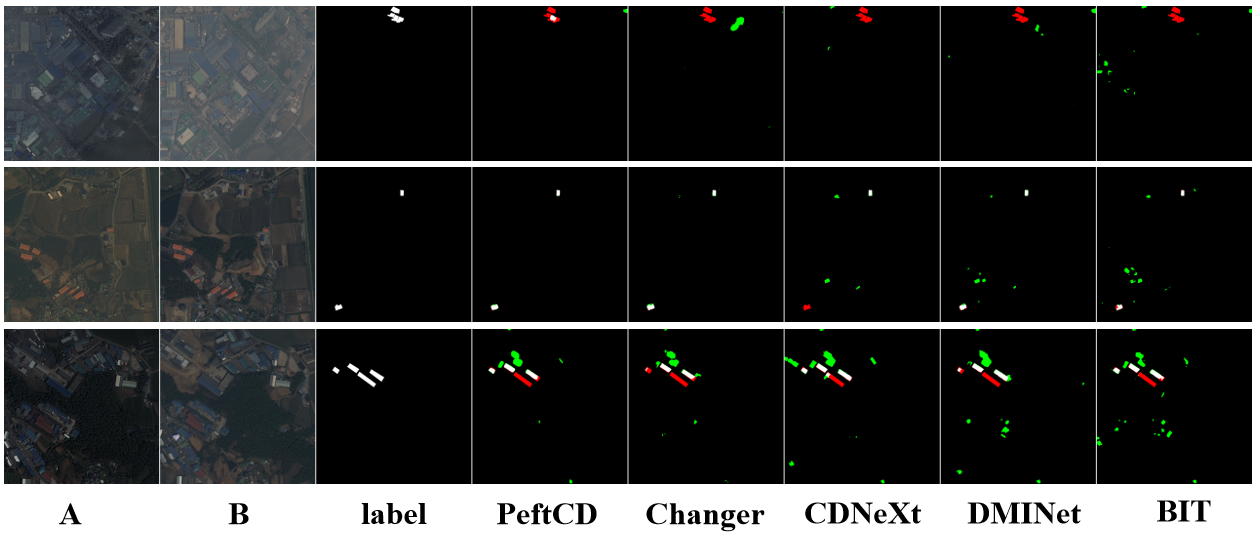
\includegraphics[width=\textwidth]{paper_figures/基于AI基础模型微调的变化检测模型研究/PeftCD/peftcd_s2looking.png}
  \caption{PeftCD 模型与对比模型在 S2Looking 数据集上的可视化对比结果}
  \label{fig:peftcd_s2looking}
\end{figure}



\paragraph{基于交换的特征交互}
在特征交互阶段,我们遵循SEED范式,摒弃了传统的差异计算模块(如特征相减或拼接融合),转而采用特征层交换(Feature Layer Exchange)机制。具体而言,从编码器输出的两组特征金字塔中,部分层级(例如,偶数层)的特征图在两个处理流之间进行交换,而其他层级(例如,奇数层)则保持不变。通过这种方式,我们得到了两组新的“混合时相”特征金字塔。这一操作的核心目的,是为后续的解码器创造一个必须解决“时空特征不一致性”的学习任务。随后,这两组混合特征金字塔被送入一个共享权重的特征金字塔网络(Shared FPN),以增强跨尺度的特征融合,为解码阶段提供更丰富的特征表示。

\paragraph{孪生解码与监督}
解码阶段同样采用共享权重的孪生解码器(Siamese Decoder)结构。每个解码器分支接收来自FPN的混合时相特征,并基于 ResBlock 构建特征提取,从而以逐层上采样的方式进行逐层特征优化和解码。
\begin{itemize}
    \item 对于未变化区域,两个时相的特征在语义和空间上高度一致,即使经过交换,解码器也能顺利重构,输出低变化概率。
    \item 对于变化区域,解码器会面临剧烈的特征冲突(例如,用“植被”的空间细节去重构“建筑”的语义),这种不一致性正是模型学习识别为“变化”的强大监督信号。
\end{itemize}
最终,两个解码器分支分别输出一个变化概率图。在训练时,这两个输出图同时受到同一个真实变化标签(Change Mask)的监督。在推理阶段,则将两个输出图进行逐像素平均,以获得更稳定和鲁棒的最终变化检测结果。



\begin{table}[!htbp]
\centering
\caption{PeftCD 与经典变化检测模型在 MSRSCD 数据集上的定量对比结果}
\label{tab:peftcd_msrscd}
\begin{tabular}{l c c c c c}
\toprule
\textbf{Model} & \textbf{OA} & \textbf{IoU} & \textbf{F1} & \textbf{Rec} & \textbf{Prec} \\
\midrule
STANet~\cite{chen_spatial-temporal_2020} & 91.44 & 54.52 & 70.57 & 69.46 & 71.71 \\
SGSLN~\cite{zhao_exchanging_2023} & 92.52 & 56.28 & 73.36 & 69.73 & 77.39 \\
ChangeFormer~\cite{bandara2022transformer} & 91.86 & 56.96 & 72.58 & 72.94 & 72.22 \\
FCCDN~\cite{Chen2021FCCDNFC} & 92.36 & 57.94 & 73.37 & 71.30 & 75.56 \\
AANet~\cite{Hang2024AANetAA} & 92.17 & 59.23 & 74.40 & 77.03 & 71.94 \\
EATDer~\cite{Ma2024EATDerEA} & 91.47 & 59.29 & 74.44 & 84.17 & 66.73 \\
MSNet~\cite{Liu2025NetworkAD} & 93.03 & 59.80 & 75.74 & 74.73 & 76.79 \\
DMINet~\cite{feng_change_2023} & 93.05 & 61.24 & 75.96 & 74.37 & 77.63 \\
BASNet~\cite{z_wang_bitemporal_2024} & 92.87 & 61.31 & 76.02 & 76.51 & 75.53 \\
CDNeXt~\cite{wei_robust_2024} & 93.24 & 61.59 & 76.23 & 73.42 & 79.27 \\
DFFNet~\cite{Liu2025FullScaleCD} & 93.23 & 61.82 & 77.44 & 78.69 & 76.22 \\
\midrule
PeftCD & 93.83 & 64.07 & 78.10 & 74.19 & 82.44 \\
\bottomrule
\end{tabular}
\end{table}


\begin{figure}[!htb]
  \centering
  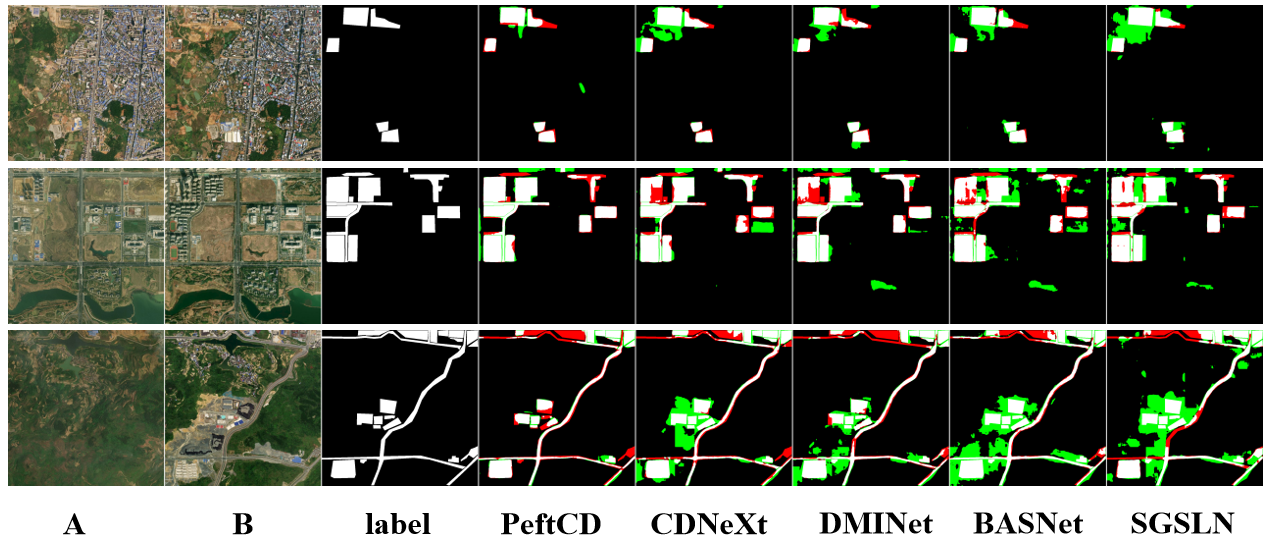
\includegraphics[width=\textwidth]{paper_figures/基于AI基础模型微调的变化检测模型研究/PeftCD/peftcd_msrscd.png}
  \caption{PeftCD 与对比模型在 MSRSCD 数据集上的可视化对比结果.}
  \label{fig:peftcd_msrscd}
\end{figure}


\begin{table}[!htb]
\centering
\caption{PeftCD 与经典变化检测模型在 MLCD 数据集上的定量对比结果}
\label{tab:peftcd_mlcd}
\begin{tabular}{l c c c c c}
\toprule
\textbf{Model} & \textbf{OA} & \textbf{IoU} & \textbf{F1} & \textbf{Rec} & \textbf{Prec} \\
STANet~\cite{chen_spatial-temporal_2020}         & 86.97 & 60.87 & 75.67 & 73.4  & 78.09 \\
ISDANet~\cite{h_ren_interactive_2025}            & 88.3  & 66.52 & 79.89 & 84.2  & 76    \\
EFI-SAM~\cite{Huang2025SAMBasedEF}          & -- & 67.72 & 80.75 & -- & -- \\
DARNet~\cite{li_densely_2022}         & 90.24 & 69.05 & 81.69 & 78.84 & 84.75 \\
BASNet~\cite{z_wang_bitemporal_2024}         & 90.51 & 70.55 & 82.73 & 82.29 & 83.17 \\
BIT~\cite{chen_remote_2022}            & 91.23 & 72.02 & 83.73 & 81.74 & 85.83 \\
DMINet~\cite{feng_change_2023}         & 91.94 & 74.03 & 85.08 & 83.18 & 87.07 \\
\midrule
PeftCD & 92.94 & 76.89 & 86.93 & 85.02 & 88.94 \\
\bottomrule
\end{tabular}
\end{table}

\begin{figure}[!htb]
  \centering
  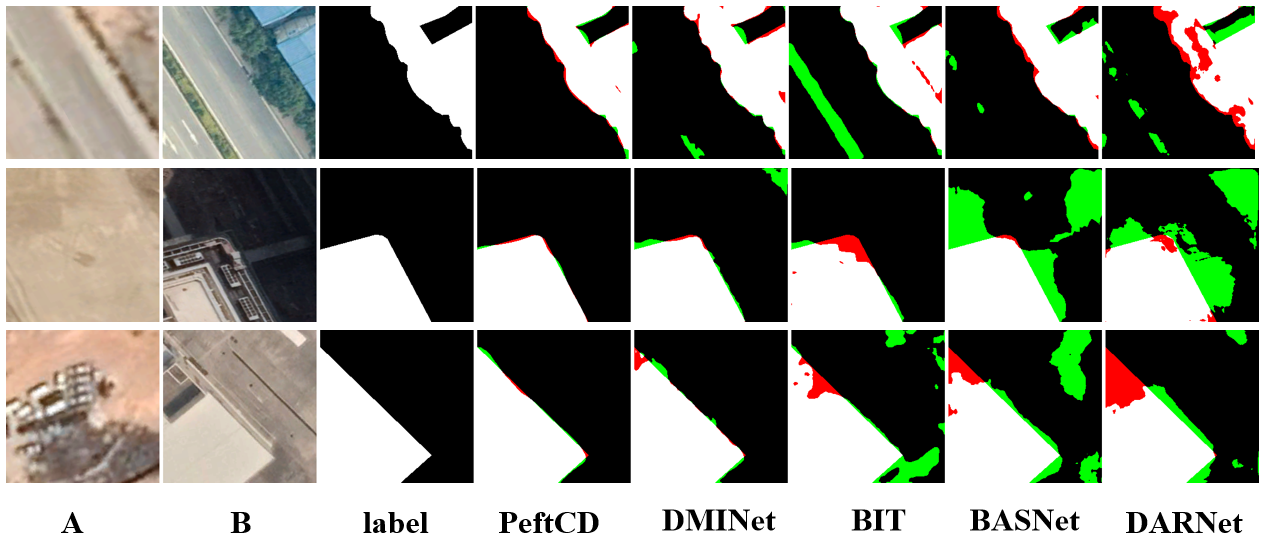
\includegraphics[width=\textwidth]{paper_figures/基于AI基础模型微调的变化检测模型研究/PeftCD/peftcd_mlcd.png}
  \caption{PeftCD 与对比模型在 MLCD 数据集上的可视化对比结果.}
  \label{fig:peftcd_mlcd}
\end{figure}


\subsubsection{基于 DINOv3 的 PeftCD架构}

我们还在 DINOv3 上实例化了 PeftCD(见图~\ref{fig:peftcd_dino3cd})。与 SAM2 不同,DINOv3 并非面向分割设计,其在 patch embedding 之后以固定空间分辨率进行运算,在各层中均输出同尺度特征。根据表~\ref{tab:peftcd_cfg} 的设置,每个 Transformer 块均通过 LoRA 注入至 MHSA 的 \texttt{qkv} 投影($r{=}8$, $\alpha{=}32$, dropout $0.1$),或通过前置残差 Adapter MLP(瓶颈维度 $32$,激活函数为 GELU)进行适配。在此过程中,骨干网络权重保持冻结,仅有 PEFT 模块参数参与训练。在使用共享权重对双时相图像进行编码后,我们执行特征层交换,以增强双时相之间的交互。解码器随后依次执行:(i) 同尺度多层特征的深度注意力融合;(ii) 基于 ASPP 的上下文增强;以及 (iii) 渐进式上采样,最终生成变化检测结果图。该设计弥补了 ViT 类骨干缺乏空间金字塔结构的不足,同时保留了 DINOv3 在语义表征和跨域泛化方面的优势。  



\subsection{基于同尺度多层融合与上下文增强的解码器}

传统的基于卷积神经网络(CNN)的编码器-解码器架构,通常依赖于编码器生成的多尺度特征金字塔(Feature Pyramid Network, FPN)。这些由不同下采样阶段产生的特征图,既包含了高层语义信息(深层、低分辨率特征),也保留了精细的空间细节(浅层、高分辨率特征),为解码器逐层恢复分辨率和精确分割提供了关键信息~\cite{lin_feature_2017}。

然而,当采用以 DINO 或其他视觉 Transformer(ViT)为代表的视觉基础模型作为编码器主干时,这一经典范式面临挑战。ViT 架构在初始的“块嵌入”(Patch Embedding)阶段,便将输入图像直接下采样 16 倍,并将图像块序列化。后续的所有 Transformer 块均在这一固定分辨率(例如 $H/16 \times W/16$)上进行特征变换与信息交互。虽然不同 Transformer 层的输出特征捕获了从低级到高级的不同层次语义,但它们在空间分辨率上是单一的,并未形成传统意义上的特征金字塔。这种架构特性导致解码器在进行上采样时,严重缺乏多尺度的空间信息,特别是对于恢复物体边界和细微变化至关重要的高频细节,从而可能导致预测结果边缘模糊、小目标丢失等问题。

为了解决 ViT 骨干网络缺乏特征金字塔的问题,我们设计了一种专门的解码器(Multi-Layer Fusion and Contextual Enhancement, MFCE)。该解码器不依赖于多尺度的空间输入,而是通过两个核心步骤,在单尺度特征图上构建强大的特征表示,并以此为基础进行上采样恢复。首先,为了在解码阶段充分利用不同层级的特征信息,对来自 ViT 不同层的同尺度特征进行深度注意力融合。其次,为了在解码阶段,扩展模型对影像特征的上下文理解能力,利用空洞空间金字塔池化(ASPP)模块构建感受野金字塔以增强上下文信息。由此,解码端的输入特征既融合了不同层级的特征信息,同时也获取了丰富的多尺度上下文感知能力。最后,解码器通过渐进式上采样路径,逐步恢复分辨率并生成最终的变化检测结果。

\subsubsection{同尺度多层特征的深度注意力融合}
尽管 ViT 的各层输出特征图分辨率相同,但它们在语义层面构成了“深度金字塔”。浅层特征更关注局部纹理和边缘,而深层特征则编码了更抽象的全局语义。为了充分且智能地利用这些信息,解码器的首要任务是对其进行高效融合。

我们为此设计了一个深度注意力融合模块,用以处理来自编码器不同层级的多个同尺度特征图。在本节中,参考ResNet与Swin Transformer等模型的架构设计方法,选用5,11,17,23层的输出作为同尺度特征图融合输入。对于输入的 4 个特征图 $\{F_1, F_2, F_3, F_4\}$,其中 $F_i \in \mathbb{R}^{B \times C_i \times H \times W}$,该模块首先将它们投影到统一的中间维度 $C_{mid}$,得到 $\{X_1, X_2, X_3, X_4\}$。随后,为每个空间位置 $(h, w)$ 的每个特征层 $X_i$ 学习一个注意力权重 $A_i(h, w)$。该权重由一个 $1 \times 1$ 卷积网络生成,并通过沿深度(层)维度的 Softmax 函数进行归一化:
\begin{equation}
    A_i(h, w) = \frac{\exp(S_i(h, w))}{\sum_{j=1}^{N} \exp(S_j(h, w))}
\end{equation}
其中 $S_i$ 是从 $X_i$ 生成的分数图。最终的融合特征 $\mathbf{X}_{\text{fused}}$ 是所有特征层的加权和:
\begin{equation}
    \mathbf{X}_{\text{fused}} = \sum_{i=1}^{N} A_i \odot X_i
\end{equation}
其中 $\odot$ 表示逐元素乘法。这种空间可变的深度注意力机制,使得模型能够根据每个像素的具体内容,自适应地决定更依赖于哪一层级的语义信息(是纹理还是类别),从而生成一个信息高度浓缩的、强大的单尺度特征图。

\subsubsection{上下文增强与渐进式上采样}
在特征融合之后,我们利用空洞空间金字塔池化(Atrous Spatial Pyramid Pooling, ASPP)模块进一步增强特征的上下文感知能力。ASPP 在融合后的特征图上并行应用多个不同膨胀率的深度可分离空洞卷积。这能够在不改变特征图分辨率的前提下,捕获多尺度的上下文信息,构建出一个“感受野金字塔”(receptive field pyramid),有效弥补了原始骨干网络在空间尺度多样性上的不足,为后续的上采样提供了更鲁棒的语义信息。

最后,经过上下文增强的特征图(分辨率仍为 $1/16$)将进入一个渐进式上采样路径。该路径通过三次“双线性插值上采样 + 深度可分离卷积”的组合,将分辨率从 $1/16$ 逐步提升至 $1/8$、$1/4$,并最终恢复到原始尺寸。其中的深度可分离卷积模块用于在上采样后平滑和优化特征,以此获取更丰富的细节信息。最终,由预测头生成像素级的变化检测结果。

\begin{table}[!htb]
\centering
\caption{PeftCD 与经典变化检测模型在 CDD 数据集上的定量对比结果}
\label{tab:peftcd_cdd}
\begin{tabular}{l c c c c c}
\toprule
\textbf{Model} & \textbf{OA} & \textbf{IoU} & \textbf{F1} & \textbf{Rec} & \textbf{Prec} \\
\midrule
BASNet~\cite{z_wang_bitemporal_2024} & 99.18 & 93.29 & 96.53 & 96.30 & 96.76 \\  
UA-BCD~\cite{li_overcoming_2025}     & --    & 93.49 & 96.64 & 96.90 & 96.38 \\
RCDT~\cite{lu_cross_2024}                  & --    & 93.79 & 96.80 & 96.97 & 96.63 \\
CDMamba~\cite{zhang_cdmamba_2025}    & 99.26 & 93.93 & 96.87 & 96.84 & 96.90 \\
SFFCE-CD~\cite{y_xing_sffce-cd_2025}   & 99.29 & 94.42 & 97.13 & 96.94 &  97.32 \\
ELGCNet~\cite{m_noman_elgc-net_2024}   & 99.33  &  94.50   & 91.17  & --   & -- \\   
DgFA~\cite{f_zhou_dual-granularity_2025} & 99.41 & 95.12 & 97.50 & 97.60 & 97.40 \\
GASNet~\cite{zhang_global-aware_2023}  & 99.41  & 95.34  & 97.61  & 98.06  & 97.17 \\
DEDANet~\cite{Li2025DifferenceEA} & 99.40 & 95.46 & 97.67 & 97.14 & 98.22 \\
DSCRNet ~\cite{Zhang2025ADS} & -- & 95.46 & 97.68 & 97.85 & 97.51 \\
CD-STMamba~\cite{Liu2025CDSTMambaTR} & 99.41 & 95.56 & 97.73 & 97.45 & 98.01 \\
MLDFNet~\cite{d_sidekejiang_mldfnet_2025}  & -- & 95.78 & 97.84 & 97.97 & 97.72 \\
ScratchFormer~\cite{Noman2023RemoteSC}   & 99.50 & 95.85  & 97.88 & -- & -- \\ 
FTransDF-Net~\cite{li_dual_2025}   & -- & 95.85 &  97.88 & 97.63 & 98.13 \\
DSFI-CD~\cite{x_li_dsfi-cd_2025}  & 99.52 & 96.10 &  98.01 & 98.34 & 97.68 \\
HASNet~\cite{c_tao_hasnet_2025}        & 99.56 & 96.49 & 98.21 & 98.12 & 98.32 \\
\midrule
PeftCD & 99.63 & 97.01 & 98.48 & 98.30 & 98.67 \\
\bottomrule
\end{tabular}
\end{table}

\begin{figure}[!htb]
  \centering
  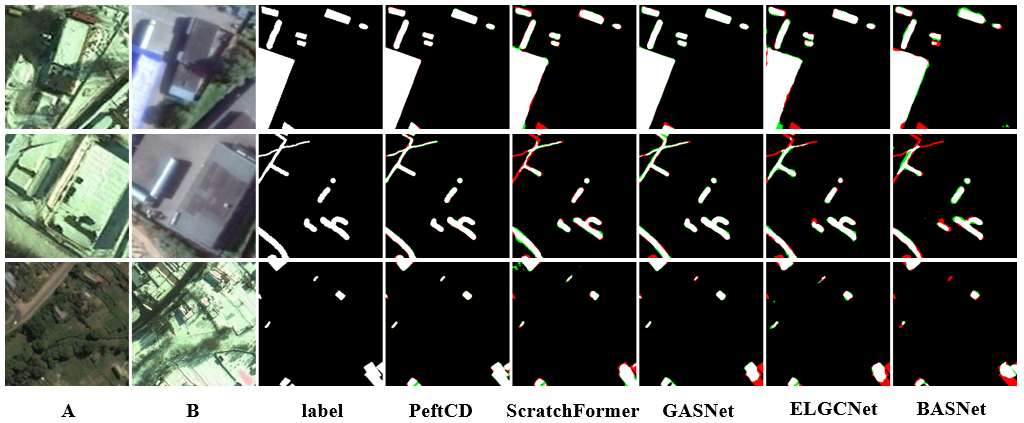
\includegraphics[width=\textwidth]{paper_figures/基于AI基础模型微调的变化检测模型研究/PeftCD/peftcd_cdd.png}
  \caption{PeftCD 与对比模型在 CDD 数据集上的可视化对比结果.}
  \label{fig:peftcd_cdd}
\end{figure}

\subsection{实验结果与分析}
\subsubsection{实验结果量化指标与可视化分析}

我们在七个具有挑战性的数据集上进行了全面的定量实验,包括 SYSU-CD、WHUCD、MSRSCD、CDD、S2Looking、LEVIR-CD 和 MLCD,以全面评估所提出 PeftCD 框架的有效性,并将其与具有代表性的先进变化检测方法进行对比。如表~\ref{tab:peftcd_sysu}、~\ref{tab:peftcd_whucd}、~\ref{tab:peftcd_s2looking}、~\ref{tab:peftcd_msrscd}、~\ref{tab:peftcd_mlcd}、~\ref{tab:peftcd_cdd} 和~\ref{tab:peftcd_levir} 所总结的结果显示,我们的方法具有显著的优越性。在所有数据集上,结合 PEFT 策略的 PeftCD 明显优于传统的 CNN 与 Transformer 基线模型,并在性能上达到或超过当前最先进方法(SOTA)。  

更具体而言,在 SYSU-CD、WHUCD、MSRSCD、CDD、S2Looking 和 MLCD 上,PeftCD 分别取得了 73.81\%、92.05\%、64.07\%、97.01\%、52.25\% 和 76.89\% 的 IoU,均超过了所有对比方法。在 SYSU-CD 上,PeftCD 将 IoU 提升 2.71 个百分点至 73.81\%,并实现了 84.93\% 的 F1 分数,显著高于亚军 ChangeMamba(83.11\%)。在 WHUCD 上,PeftCD 达到 92.05\% 的 IoU,超过 EfficientCD 1.34 个百分点,并获得 96.79\% 的 Precision,表明其对误报具有很强的抑制能力。在 S2Looking 上,PeftCD 取得了 52.25\% 的 IoU,优于 Conv-former(51.51\%)。这些结果表明,PeftCD 在复杂变化场景中表现出色,能够有效捕获多样化的变化模式。  



\begin{table}[!htb]
\centering
\caption{PeftCD 模型与经典变化检测模型在 LEVIR-CD 数据集上的定量对比结果}
\label{tab:peftcd_levir}
\begin{tabular}{l c c c c c}
\toprule
\textbf{Model} & \textbf{OA} & \textbf{IoU} & \textbf{F1} & \textbf{Rec} & \textbf{Prec} \\
\midrule
    STANet~\cite{chen_spatial-temporal_2020}   & 99.02 & 81.85 & 90.02 & 87.13 & 93.10 \\
    MSCANet~\cite{m_liu_cnn-transformer_2022}          &  99.03 &  81.91 &  90.06 &  86.38 &  94.06  \\
    MFATNet~\cite{Mao2022MFATNetMF}          &  99.03 &  82.42 &  90.36 &  88.93 &  91.85  \\
    ChangeFormer~\cite{bandara2022transformer}     &  99.04 &  82.66 &  90.50 &  90.18 &  90.83  \\
    P2V~\cite{lin_transition_2023}              &  99.04 &  83.00 &  90.71 &  91.78 &  89.67  \\
    CDMamba~\cite{zhang_cdmamba_2025}          &  99.06 &  83.07 &  90.75 &  90.08 &  91.43  \\
    AMTNet~\cite{Liu2023AnAM}           &   --   &  83.08 &  90.76 &  89.71 &  91.82  \\
    B2CNet~\cite{Zhang2024B2CNetAP} & 99.10 & 83.72 & 91.14 & 91.01 & 91.27 \\
    DgFA~\cite{f_zhou_dual-granularity_2025}   & 99.11 & 83.93 & 91.26 & 90.84 & 91.69 \\
    HATNet~\cite{Xu2024HybridAT} & 99.13 & 84.12 & 91.38 & 90.15 & 92.64 \\
    DMATNet~\cite{Song2022RemoteSI}          &  98.25 &  84.13 &  90.75 &  89.98 &  91.56  \\
    DEDANet~\cite{Li2025DifferenceEA}          &  99.14 &  84.18 &  91.41 &  90.06 &  92.80  \\
    STransUNet~\cite{Yuan2022STransUNetAS}       &  99.13 &  84.19 &  91.41 &  90.55 &  92.30  \\
    LCCDMamba~\cite{Huang2025LCCDMambaVS}       &  99.16 &  84.64 &  91.68 &  92.42 &  90.96  \\
    AGFormer~\cite{Chen2025AGFormerAA}         &  99.17 &  84.81 &  91.78 &  90.84 &  92.74  \\
    DSCRNet~\cite{Zhang2025ADS}         &  -- &  85.15 &  91.98 &  92.43 &  91.53  \\
    HCGMNet~\cite{Han2023HCGMNetAH}          &  99.18 &  85.26 &  92.04 &  92.81 &  91.29  \\
    Changer~\cite{Fang2022ChangerFI}        &   --   &  85.29 &  92.06 &  90.56 &  93.61  \\
    DMFANet~\cite{Zhan2025DifferenceAwareMF}         &  99.20 &  85.33 &  92.09 &  90.93 &  93.27  \\
    CGNet~\cite{han_change_2023}            &  99.20 &  85.40 &  92.13 &  91.93 &  92.32  \\
    EfficientCD~\cite{dong_efficientcd_2024} &  99.22 &  85.55 &  92.21 &  91.22 &  93.23  \\
    FTA-Net~\cite{t_zhu_fta-net_2025}   & -- & 85.58 & 92.23 & 92.68 & 91.79 \\
\midrule
PeftCD  & 99.22 & 85.62 & 92.25 & 91.44 & 93.08 \\
\bottomrule
\end{tabular}
\end{table}

\begin{figure}[!htb]
  \centering
  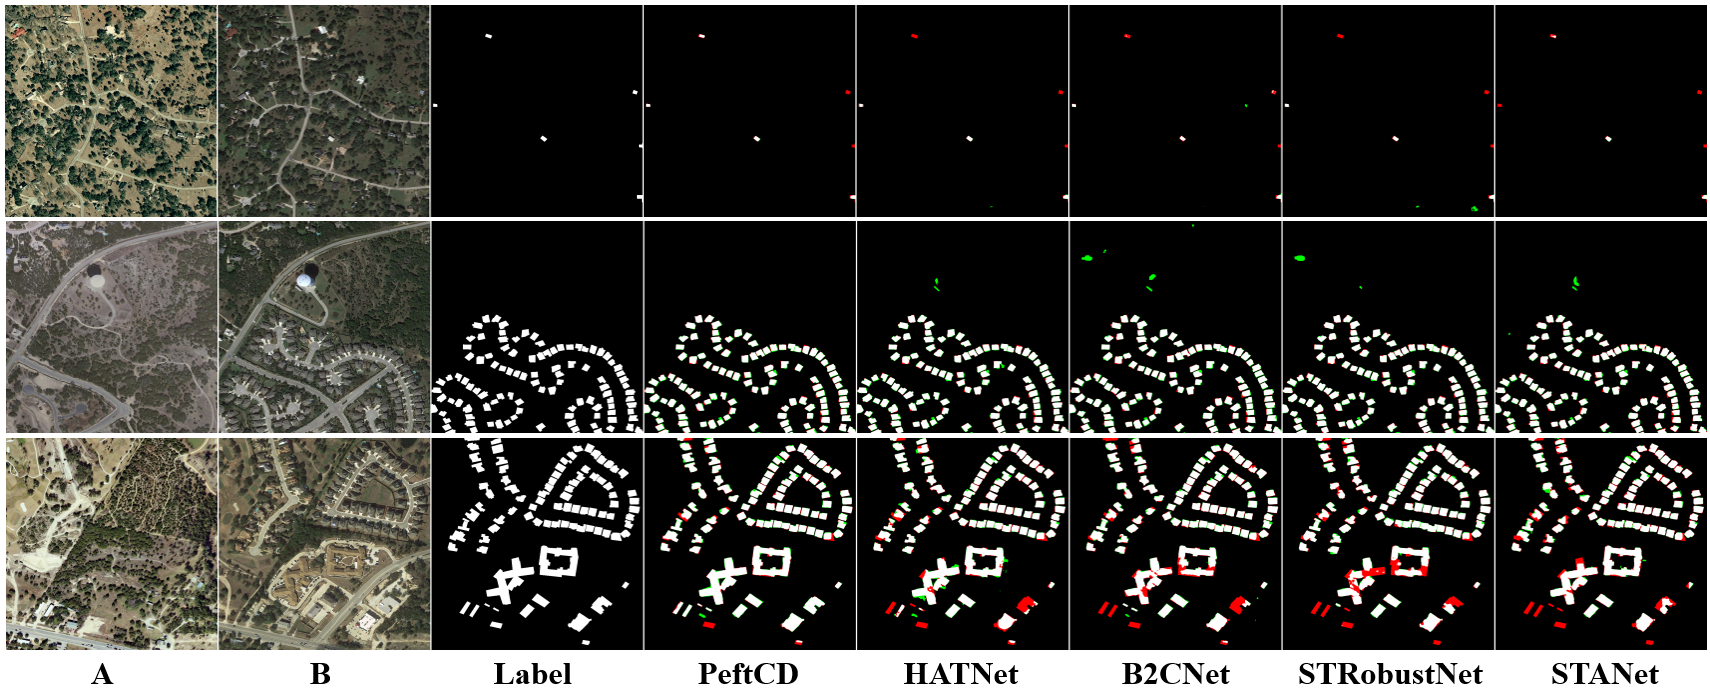
\includegraphics[width=\textwidth]{paper_figures/基于AI基础模型微调的变化检测模型研究/PeftCD/peftcd_levir.png}
  \caption{PeftCD 与对比模型在 LEVIR-CD 数据集上的可视化对比结果.}
  \label{fig:peftcd_levir}
\end{figure}


为了进一步展示 PeftCD 在实际检测中的优势,我们在图~\ref{fig:peftcd_sysu}、~\ref{fig:peftcd_whucd}、~\ref{fig:peftcd_s2looking}、~\ref{fig:peftcd_msrscd}、~\ref{fig:peftcd_mlcd}、~\ref{fig:peftcd_cdd} 和~\ref{fig:peftcd_levir} 中提供了定性对比。在这些可视化结果中,白色像素表示正确检测的变化区域(TP),黑色表示正确检测的非变化区域(TN),绿色表示误报(FP),红色表示漏检(FN)。  

从定性结果可以看出,PeftCD 在多个方面均显著优于对比方法。首先,它能够更完整地识别变化区域,明显减少漏检(红色),尤其是在小目标和不规则形状的场景中(如 SYSU-CD 中的分散建筑和 WHUCD 中的小型独立建筑)。其次,它能够提供更精确、边界更平滑的变化区域分割,有效缓解其他模型常见的边界模糊或锯齿化伪影。最重要的是,PeftCD 在抑制背景噪声和伪变化方面表现出很强的鲁棒性,几乎没有误报(绿色)。我们将这些优势归因于视觉基础模型强大的语义理解与泛化能力,使其能够更好地区分真实地物覆盖变化与由光照、季节或其他环境因素引起的外观变化。综上所述,定量与定性分析均一致表明,PeftCD 在检测精度、完整性与鲁棒性方面均达到了领先水平。  


\subsubsection{消融实验}

如表~\ref{tab:peftcd_ablation} 所示,PEFT在两类骨干网络(SAM2 与 DINOv3)上均较 Frozen Encoder 基线取得了稳定提升,这表明即使在冻结大部分参数的情况下,仅注入少量可训练模块也能够有效地引导模型适配“变化”这一概念。总体而言,\textbf{DINOv3+LoRA} 在大多数数据集上取得了最佳或并列最佳的 IoU:在 SYSU-CD、WHUCD、S2Looking、MSRSCD 上分别达到 73.81、92.05、52.25、64.07,相较于冻结基线有显著提升。在 \textbf{MLCD} 上,\textbf{DINOv3+Adapter} 略优于 LoRA(76.89 vs.\ 76.54),说明 \textbf{Adapter} 在地貌变化复杂、尺度分布更丰富的数据集上展现出更好的鲁棒性。相比之下,\textbf{SAM2} 骨干在 \textbf{LEVIR-CD} 和 \textbf{CDD} 上展现出更明显的优势:\textbf{SAM2+LoRA} 在 LEVIR-CD 上达到 85.62,而 \textbf{SAM2+Adapter} 在 CDD 上取得了 \textbf{97.01} 的最佳 IoU,反映了大规模分割先验在建筑物边界刻画和季节性外观变化抑制方面的积极作用。综上所述,\textbf{DINOv3+LoRA} 能够提供跨场景的一致性优势,这主要归因于 DINOv3 在更大规模和更丰富语料上的预训练所带来的更强泛化能力;而 \textbf{SAM2} 则在特定场景下展现出更优的边界识别能力。

此外,为进一步验证 DINO3CD 架构中多层融合与上下文增强解码器设计的有效性,我们进行了第二组消融实验,专门评估了所提出的多层融合与上下文增强(MFCE)解码器的贡献。如表~\label{tab:peftcd_dino3cd_ablation}所示,其中,BaseLine为对DINOv3中的四层特征图进行特征细化与均值融合,最后采用四级逐级上采样的解码器,MFCE则为本节提出的多层融合与上下文增强解码器。实验结果表明,无论采用 Adapter 还是 LoRA 微调策略,MFCE 解码器相较于仅对最后一层特征进行上采样的基线(Baseline)解码器,均表现出显著的性能优势。这证实了我们的观点:对于缺乏天然特征金字塔的 ViT 类骨干网络,MFCE 解码器通过有效融合多层级同尺度特征并增强上下文感知,成功弥补了其在空间细节恢复上的不足,从而生成了更精细、更准确的变化检测结果。

\begin{table}[!htb]
\centering
\small
\setlength{\tabcolsep}{3pt} % 调整列间距
\caption{不同主干模型与参数高效微调(PEFT)方法的消融实验结果(IoU \%)}
\label{tab:peftcd_ablation}
\begin{tabularx}{\textwidth}{p{1.8cm} p{2.5cm} *{7}{c}}
\toprule
\textbf{Backbone} & \makecell{\textbf{Fine-tuning}\\\textbf{Method}} & \makecell{\textbf{SYSU-}\\\textbf{CD}} & \textbf{WHUCD} & \textbf{S2Looking} & \textbf{MSRSCD} & \textbf{MLCD} & \makecell{\textbf{LEVIR-}\\\textbf{CD}} & \textbf{CDD} \\
\midrule
\multirow{3}{*}{SAM2}
& Frozen Encoder & 69.45 & 87.83 & 47.98 & 60.42 & 73.49 & 83.58 & 95.95 \\
& Adapter        & 71.91 & 91.81 & 49.97 & 63.15 & 75.73 & 85.60 & 97.01 \\
& LoRA           & 72.51 & 90.86 & 50.59 & 62.31 & 74.98 & 85.62 & 96.99 \\
\midrule
\multirow{3}{*}{DINOv3}
& Frozen Encoder & 71.02 & 90.97 & 50.20 & 62.93 & 75.17 & 80.83 & 92.04 \\
& Adapter        & 73.36 & 91.93 & 51.29 & 63.28 & 76.89 & 84.68 & 95.74 \\
& LoRA           & 73.81 & 92.05 & 52.25 & 64.07 & 76.54 & 85.32 & 95.58 \\
\bottomrule
\end{tabularx}
\end{table}

\begin{table}[!htb]
\centering
\small
\setlength{\tabcolsep}{3pt} % 调整列间距
\caption{DINO3CD中多层融合与上下文增强解码器的消融实验结果(IoU \%)}
\label{tab:peftcd_dino3cd_ablation}
\begin{tabularx}{\textwidth}{p{1.8cm} p{2.5cm} *{7}{c}}
\toprule
\textbf{Backbone} & \makecell{\textbf{Fine-tuning}\\\textbf{Method}} & \makecell{\textbf{SYSU-}\\\textbf{CD}} & \textbf{WHUCD} & \textbf{S2Looking} & \textbf{MSRSCD} & \textbf{MLCD} & \makecell{\textbf{LEVIR-}\\\textbf{CD}} & \textbf{CDD} \\
\midrule
\multirow{2}{*}{Adapter} 
& Baseline & 70.66 & 90.96 & 49.42 & 61.83 & 75.42 & 83.69 & 94.87 \\
& MECE     & 73.36 & 91.93 & 51.29 & 63.28 & 76.89 & 84.68 & 95.74 \\
\midrule
\multirow{2}{*}{LoRA}    
& Baseline & 72.52 & 90.16 & 50.58 & 62.59 & 75.48 & 84.45 & 94.82 \\
& MECE     & 73.81 & 92.05 & 52.25 & 64.07 & 76.54 & 85.32 & 95.58 \\
\bottomrule
\end{tabularx}
\end{table}


\subsection{PeftCD架构的局限性与未来方向}
\subsubsection{基于单尺度 ViT 骨干的解码}
以 DINOv3 为代表的 ViT 骨干在固定的 $1/16$ 分辨率下进行深层特征变换,因而天然缺乏 CNN/FPN 式的多尺度空间金字塔。这一局限带来了两个典型问题:(i)在上采样过程中,边界和小目标容易产生空间混叠与锯齿化伪影;(ii)当仅依赖单尺度全局语义时,局部几何与纹理差异往往被削弱,而这些差异恰是变化检测的关键证据。为此,本节设计了一种基于“同尺度多层深度注意力融合 + ASPP 上下文增强 + 渐进式上采样”的解码器,在不改变主干分辨率的前提下弥补语义与几何之间的落差。尽管同尺度多层融合显著缓解了单尺度瓶颈,但仍然存在以下问题:(i)由于 $1/16$ 下采样带来的分辨率上限,对小目标的刻画仍受限制;(ii)ASPP 的固定膨胀率限制了其对不同尺度目标的自适应性;(iii)在大规模模型中,多层融合带来了相对较高的计算与存储开销。我们认为,未来工作可以进一步改进单尺度 ViT 解码器:(i)设计更高效的多层融合模块,或引入轻量级的跨层交互机制;(ii)结合辅助特征编码分支,以捕获更精细的图像细节。

\subsubsection{变化检测的 PEFT 策略}
本节系统评估了 LoRA 与 Adapter 两种参数高效微调(PEFT)策略在变化检测中的表现。实验结果表明,这两种方法在保持骨干冻结的前提下,均能显著提升性能,尤其是在 WHUCD 和 CDD 等大规模数据集上。这表明,PEFT 能够在不破坏基础模型通用能力的情况下,快速适配“变化”这一下游任务。具体而言,LoRA 在注入注意力投影层时表现出更显著的性能提升,而 Adapter 由于其瓶颈设计,在不同 Transformer 层的插入中展现出更强的灵活性。然而,PEFT 在变化检测中仍存在一定局限性:(i)当变化模式与预训练任务差异较大时(如 S2Looking 的侧视影像),PEFT 的适配能力相对有限,难以完全弥合域间差距;(ii)LoRA 与 Adapter 大多是独立注入各层,其跨层交互仍然不足,导致在细粒度语义变化的边界捕捉上存在模糊;(iii)当前 PEFT 配置大多是固定的(如秩、瓶颈维度),缺乏针对数据集特性或任务复杂度的自适应调整。

\subsection{小结}
本节提出了一种新颖的变化检测框架 \textbf{PeftCD},通过结合视觉基础模型(如 SAM2、DINOv3)与参数高效微调(PEFT)策略,有效解决了遥感影像中的伪变化干扰与泛化困难。该方法通过冻结骨干的大部分参数,仅训练少量新增模块,成功地将基础模型的强大先验知识迁移到变化检测任务中。基于 SYSU-CD、WHUCD 等七个公开数据集的实验表明,PeftCD 在多项指标上均取得了最先进的性能,尤其在变化边界刻画与伪变化抑制方面表现突出。总体而言,本节验证了 PeftCD 作为一种高效范式在精度、效率与泛化性之间的良好平衡,并为大规模基础模型在实际遥感应用中的落地提供了有价值的参考。

% 
\chapter{基于双时相遥感影像特征交互的变化检测算法研究}
在变化检测任务中,基于深度学习的变化检测模型通常是在编码阶段,分别对双时相图像进行特征提取,然后基于双时相特征进行融合,以使得融合特征能够更好地表征变化信息。在本文中,将这种使用双时相影像特征融合或者交互表征变化特征的方法成为特征交互。在变化检测任务中,通常双时相特征交互的方法主要分为三种:一种是结合数学计算表现双时相特征图差异,比如结合向量距离计算~\cite{dong2024changeclip},差值计算~\cite{h_wei_spatio-temporal_2024}以及绝对值计算~\cite{shi_deeply_2022}等。第二种是基于注意力机制的特征交互方法,比如自注意力机制~\cite{Ying2024DGMA2NetAD}以及交叉注意力机制~\cite{lu_cross_2024}等。第三种是结合神经网络模块进行特征交互,比如特征拼接~\cite{chen2024changemamba}、特征交换~\cite{Fang2022ChangerFI}以及其他复杂的网络模块设计方法~\cite{Zhu2025Change3DRC}等。在本章中,重点针对第一种和第三种提出了本文的解决办法,分别从数学距离度量、特征交换以及复杂网络模块设计方法研究了表征变化特征的方法。

\section{基于特征层交换与欧氏距离差异特征计算的变化检测方法}
\subsection{引言}

遥感影像变化检测在环境监测、城市发展和水利领域中起着至关重要的作用。近年来,深度学习技术在遥感影像处理中的应用取得了显著进展。通过利用深度学习模型强大的特征拟合能力和高性能计算设备,遥感影像变化检测的准确性和效率得到了显著提升~\cite{Chen2021FCCDNFC}。这些深度学习模型能够处理大规模的遥感数据,识别和分析细微的地表变化,从而在环境监测中发挥越来越重要的作用。在遥感影像变化检测的深度学习领域,许多研究者从不同的研究层面优化了变化检测算法~\cite{chen_remote_2022, Fang2022ChangerFI}。变化检测算法的核心目标是检测双时相影像中发生变化的区域,模型需要识别在不同时间拍摄的两幅影像之间的变化区域。为了实现这一目标,可以关注两个主要方向:首先,增强模型从双时相影像中提取特征的能力,从而提高其对遥感影像的表示能力;其次,设计更精细的模块来表达差异特征,使变化检测模型更容易识别双时相影像中的变化区域。

具体而言,在特征提取骨干网络方面,一些研究者选择了先进的视觉变换器Vision Transformer~\cite{Dosovitskiy2020AnII}来提取双时相影像的特征。通过这些骨干网络强大的特征提取能力,模型在变化检测任务中的性能得到了提升~\cite{He2015DeepRL, Gu2023MambaLS, Dosovitskiy2020AnII}。与此同时,考虑到变化检测的独特性,许多研究者集中于差异特征的计算~\cite{dong_changeclip_2024, dong_efficientcd_2024}。因此,前述两类研究从不同的角度优化了变化检测任务。前者增强了模型对遥感影像中不同地物目标的理解,使得模型能够更好地识别双时相影像中的各种地物类别;后者则增强了模型对变化特征的感知能力,这是变化检测任务的基础。

\begin{figure}[!htbp]
  \centering
  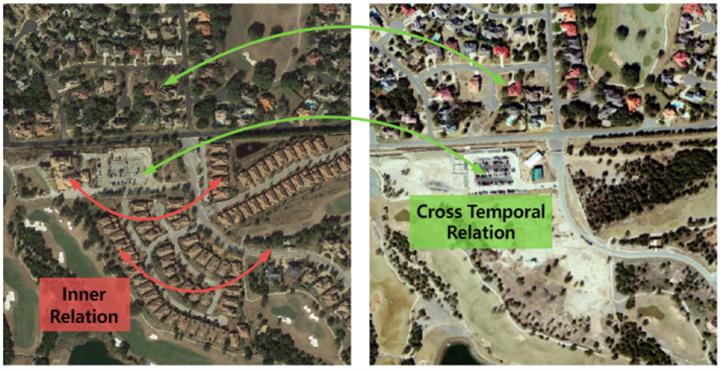
\includegraphics[width=\textwidth]{paper_figures/基于双时相遥感影像特征交互的变化检测算法研究/EfficientCD/efficientcd_relation.png}
  \caption{变化检测任务中的像素关系示意图}
  \label{fig:efficientcd_relation}
\end{figure}

在常见的变化检测算法中,通常使用拼接、加法和减法等方法来融合双时相特征,表示差异特征。从计算角度来看,特征拼接并不能直接反映双时相特征图之间的差异,它主要通过模型与变化标签之间的强拟合关系来学习变化区域~\cite{Daudt2018FullyCS}。加法保留了双时相影像中的前景区域,但模型需要学习哪些前景区域代表变化区域~\cite{gu2023fdff}。减法消除了双时相影像中相同元素的影响~\cite{feng_change_2023}。然而,减法方法增加了变化特征的数值差异,使得模型更难区分变化区域。因此,设计一种适合的方式来更好地构建差异特征的表示,一直是变化检测领域的研究热点。

在语义分割领域,特别是遥感影像分割中,不同层次特征的融合显著提高了模型的性能~\cite{Dong2021AMF, lin_feature_2017}。这些特征融合策略通过整合网络不同深度的信息,有效增强了模型识别图像中不同尺度和复杂度目标的能力。在遥感影像分割中,这种方法改善了对高空拍摄影像中细节变化的处理,如小尺度表面特征和复杂地形结构,从而实现了更精确的地物分类~\cite{wang2022unetformer}和变化检测~\cite{dong_changeclip_2024}。对于变化检测任务,独特的双时相影像为多层次特征融合提供了额外的优化方向~\cite{dong_changeclip_2024, Li2023MDFENetAM}。注意到,双时相影像中的地物类别存在显著相似性,如图~\ref{fig:efficientcd_relation}所示。因此,构建单时相影像内部以及双时相影像之间的像素依赖关系对增强模型的表示能力是有益的。

基于SEED架构中对变化检测任务中特征交换策略的阐述,本章提出了一种变化检测算法的优化方案,重点增强了单时相影像特征和双时相影像之间特征的交互。具体而言,本章的主要贡献如下:
\begin{itemize}
  \item 为了增强双时相遥感影像之间的特征交互,基于特征层交换的策略设计了ChangeFPN架构,通过无参数的方法改善双时相影像之间的特征传递。
  \item 基于特征图的欧几里得距离设计了一个逐层解码架构,用于变化检测任务。
\end{itemize}

\begin{figure}[!htbp]
  \centering
  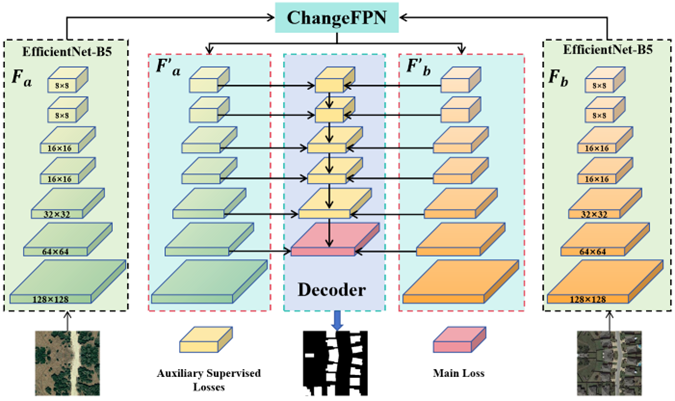
\includegraphics[width=\textwidth]{paper_figures/基于双时相遥感影像特征交互的变化检测算法研究/EfficientCD/efficientcd.png}
  \caption{EfficientCD的整体架构}
  \label{fig:efficientcd}
\end{figure}

\subsection{总体结构设计}

本章设计了一种基于EfficientNet骨干网络的变化检测网络,如图~\ref{fig:efficientcd}所示。该图展示了基于EfficientNet-B5骨干网络的变化检测模型。所提出的EfficientCD包括三部分:基于EfficientNet的特征提取骨干网络、用于促进不同层次双时相影像信息交换的ChangeFPN模块,以及逐层解码模块。骨干网络利用EfficientNet架构从输入影像中提取丰富且高效的特征,并且双编码器共享相同的权重。选择这一骨干网络是因为它在准确性和效率之间保持平衡,非常适合变化检测任务的需求,特别是在处理大型且复杂数据集时。ChangeFPN模块旨在增强从双时相影像中提取的不同层次特征之间的交互,如图~\ref{fig:efficientcd_changefpn}所示。通过允许对应层次的特征金字塔之间交换信息,ChangeFPN旨在提高模型检测和突出双时相影像之间变化的能力。最后,多层次解码模块从融合的金字塔特征图中逐步重建最终的变化检测图。这个逐层的方法确保了模型能够理解遥感影像中不同尺度的目标变化。在解码阶段,使用黄色特征图计算多个辅助损失,并使用红色特征图计算主损失。推理结果是从红色特征图中上采样得到的。

\begin{table}[!htbp]
\centering
\caption{EfficientNet-B5架构}
\label{tab:efficientnet-b5}
% 使用 booktabs 风格,移除竖线,并使用 c (居中) 和 l (左对齐)
\begin{tabular}{l l c c c c}
\toprule
\textbf{Stage} & \textbf{Operator} & \textbf{Kernel size} & \textbf{Resolution} & \textbf{Channels} & \textbf{Layers} \\
\midrule
1     & Conv       & $3\times3$     & $128\times128$  & 48       & 1      \\
2     & MBConv1    & $3\times3$     & $128\times128$  & 24       & 3      \\
3     & MBConv6    & $3\times3$     & $64\times64$    & 40       & 5      \\
4     & MBConv6    & $5\times5$     & $32\times32$    & 64       & 5      \\
5     & MBConv6    & $3\times3$     & $16\times16$    & 128      & 7      \\
6     & MBConv6    & $5\times5$     & $16\times16$    & 176      & 7      \\
7     & MBConv6    & $5\times5$     & $8\times8$      & 304      & 9      \\
8     & MBConv6    & $3\times3$     & $8\times8$      & 512      & 3      \\
\bottomrule
\end{tabular}
\end{table}


目前,大多数变化检测算法围绕视觉变换器(Vision Transformer,ViT)架构展开。视觉变换器架构中自注意力模块的全像素计算方法使得基于视觉变换器的特征提取骨干网络具备了遥感影像的全局认知能力。因此,利用视觉变换器架构的变化检测任务在多个数据集上取得了显著的成功。然而,通常由于自注意力模块中广泛的高维矩阵乘法计算,视觉变换器具有较高的计算成本。这种高计算需求也意味着模型在拟合遥感影像特征方面有更好的能力。

与上述方法不同,本章选择了轻量化网络结构EfficientNet作为变化检测任务的特征提取骨干网络。对于传统的卷积神经网络(CNNs),通过增加网络的深度和宽度来增强模型的拟合能力是可行的。然而,增加网络深度和宽度也会导致计算消耗的增加,并可能在网络训练过程中引发更严重的过拟合问题。变化检测任务通常以二分类为目标,专注于检测前景目标的变化区域。此外,与自然场景图像相比,遥感影像中包含的特定语义类别目标较少。因此,考虑到使用EfficientNet作为变化检测任务的特征提取骨干网络是合理的。为此,基于EfficientNet的结构特征,设计了图~\ref{fig:efficientcd}所示的特征提取骨干网络。选择EfficientNet-B5作为主要骨干网络,其架构结构见表\ref{tab:efficientnet-b5}。

表\ref{tab:efficientnet-b5}中提到的MBConv是架构中的一个模块,其中MBConv后面的数字(如1或6)表示扩展因子。这意味着MBConv模块中的第一个1x1卷积层会将输入特征矩阵的通道数扩展n倍。卷积核大小表示MBConv模块中深度可分离卷积~\cite{Chollet2016XceptionDL}使用的卷积核的大小。分辨率表示该阶段的输入分辨率。‘通道’指的是经过该阶段处理后输出特征矩阵中的通道数。‘层数’表示该阶段内操作结构的重复次数。

\begin{figure}[!htbp]
  \centering
  \includegraphics[width=\textwidth]{paper_figures/基于双时相遥感影像特征交互的变化检测算法研究/EfficientCD/efficientcd_changefpn.png}
  \caption{ChangeFPN中的特征交换方法示意图}
  \label{fig:efficientcd_changefpn}
\end{figure}

\subsection{结合特征层交换的变化检测FPN结构设计}

在计算机视觉领域,不同层次特征的融合增强了模型感知不同尺度目标的能力。然而,与语义分割任务不同,变化检测中的双时相影像地理位置保持不变,仅因时间变化导致影像中土地覆盖元素的差异。尽管如此,考虑到地理位置的一致性,双时相影像之间应该存在较强的相关性。为了使模型能够学习更多双时相影像之间的相关性,本章设计了ChangeFPN结构。如上图~\ref{fig:efficientcd_changefpn}所示,$F_{a}$ 和 $F_{b}$ 表示双时相影像的特征金字塔,${F}_{a}^{\prime}$ 和 ${F}_{b}^{\prime}$ 表示ChangeFPN的输出,与图~\ref{fig:efficientcd}相同。为了确保双时相影像之间信息的充分融合,本章选择了交换双时相特征金字塔相邻层的特征。 $F_{ab}$ 和 $F_{ba}$ 表示交换后的结果。同时对 $F_{ab}$ 和 $F_{ba}$ 应用了 FPN模型,生成了 ${F}_{ab}^{\prime}$ 和 ${F}_{ba}^{\prime}$。其中,$F_{ab}$ 和 $F_{ba}$ 具有彼此的特征层,通过FPN对 $F_{ab}$ 和 $F_{ba}$ 进行了多层次特征融合。最终得到的输出特征金字塔 ${F}_{ab}^{\prime}$ 和 ${F}_{ba}^{\prime}$ 融合了双时相影像的特征。通过这种计算方法,不仅加强了不同层次的信息融合,还构建了双时相影像特征图之间的信息融合。为了确保特征交换方法不会影响后续解码部分,使用了层交换计算进行恢复。与其他基于特征的方法不同,这些方法构建了双时相影像特征之间的交互,基于层次的方法巧妙地增加了双时相影像之间的信息交换,从而提高了变化检测模型感知变化特征的能力,同时没有增加计算负担。

\subsection{结合欧氏距离差异特征计算的变化检测解码器}

在EfficientCD的解码阶段,本章采用了分层的方法处理ChangeFPN输出的特征,并计算了每个层次上双时相特征图之间的变化,如图\ref{fig:efficientcd_euclidean}所示。对于FPN模块中的每一层双时相特征图,首先沿着通道维度C将双时相特征图(标记为F1和F2)拼接,形成一个合并的特征图。随后,计算这两个特征图之间的欧几里得距离,以估算双时相特征图之间的差异程度。计算欧几里得距离的公式如下:
\begin{align}
D &= \sqrt{\sum_{c}(F_{1} - F_{2})^{2}} \label{func:efficientcd-1} \\
D_{\mathrm{norm}} &= \sigma\!\Bigl(\frac{D}{D_{\max}}\Bigr) \label{func:efficientcd-2}
\end{align}


在公式(1-3)中, D表示F1和F2之间的欧几里得距离矩阵, $\sigma$表示sigmoid函数,${D_{\max}}$为欧几里得距离的最大值,$D_{\mathrm{norm}}$是归一化后的距离。在图\ref{fig:efficientcd_euclidean}中,左侧的紫色模块表示双时相特征图F1和F2。首先,双时相特征图F1和F2被拼接生成一个融合的特征图。然后,融合特征图经过一个残差块处理,同时添加来自前一层的解码特征图,构建了解码阶段的逐层特征融合。融合特征图接着经过双线性插值上采样,以恢复其空间分辨率。上采样后的特征图进一步经过另一个残差块处理。为了增强模型对变化区域的敏感性,双时相特征图F1和F2通过欧几里得距离模块计算差异图,如公式\ref{func:efficientcd-1}和\ref{func:efficientcd-2}所示。差异图也经过双线性插值上采样,以匹配特征图的分辨率。然后,上采样后的差异图和特征图逐元素相乘,增强了变化显著区域的特征。这些步骤构成了一个结合欧几里得距离的解码模块,有效提高了模型在逐层解码和特征融合中检测变化的能力。逐层解码方法更适合遥感影像密集预测任务,因为遥感图像识别通常需要结合不同层次的特征信息,以获得更好的识别效果。

\begin{figure}[!htbp]
  \centering
  \includegraphics[width=\textwidth]{paper_figures/基于双时相遥感影像特征交互的变化检测算法研究/EfficientCD/efficientcd_euclidean.png}
  \caption{结合欧几里得距离计算的双时相差异特征融合模块示意图。}
  \label{fig:efficientcd_euclidean}
\end{figure}

\begin{figure}[!htbp]
  \centering
  \includegraphics[width=\textwidth]{paper_figures/基于双时相遥感影像特征交互的变化检测算法研究/EfficientCD/efficientcd_clcd.png}
  \caption{EfficientCD 模型与对比模型在CLCD数据集上的可视化对比结果}
  \label{fig:efficientcd_clcd}
\end{figure}

\begin{figure}[!htbp]
  \centering
  \includegraphics[width=\textwidth]{paper_figures/基于双时相遥感影像特征交互的变化检测算法研究/EfficientCD/efficientcd_levir.png}
  \caption{fficientCD 模型与对比模型在 LEVIR-CD 数据集上的可视化对比结果}
  \label{fig:efficientcd_levir}
\end{figure}

\subsection{实验结果与分析}


\begin{figure}[!htbp]
  \centering
  \includegraphics[width=\textwidth]{paper_figures/基于双时相遥感影像特征交互的变化检测算法研究/EfficientCD/efficientcd_sysu.png}
  \caption{EfficientCD 模型与对比模型在 SYSU-CD 数据集上的可视化对比结果}
  \label{fig:efficientcd_sysu}
\end{figure}


\subsubsection{实验结果量化指标与可视化分析}

如表~\ref{tab:efficientcd_clcd}、表~\ref{tab:efficientcd_levir}、表~\ref{tab:efficientcd_whucd}和表~\ref{tab:efficientcd_sysu},在四个数据集上对EfficientCD进行了广泛的评估:CLCD、LEVIR-CD、WHUCD和SYSU-CD。根据主要评估指标,EfficientCD在所有数据集上均取得了最先进的性能。符号``--''表示原始论文中缺失的数据。对于这些情况,重新训练了部分模型以提高准确性。由于这些是二分类变化检测任务,前景变化类别的交并比(IoU)作为主要指标。对四个数据集性能的详细比较明确展示了EfficientCD算法在关键评估指标上的优越性。特别是在IoU指标方面,EfficientCD不仅在每个数据集上都取得了最高得分,而且还表现出了显著的优势:在CLCD数据集上,EfficientCD的IoU为65.14\%,超过第二名CGNet(62.67\%)约2.47个百分点;在LEVIR-CD数据集上,其IoU为85.55\%,略高于CGNet(85.40\%)0.15个百分点;在SYSU-CD数据集上,EfficientCD的IoU飙升至71.53\%,超过第二名SSANet(68.18\%)3.35个百分点;在WHUCD数据集上,EfficientCD的IoU为90.71\%,超越CGNet(90.41\%)0.3个百分点。这些比较数据突显了EfficientCD在精确识别遥感影像中的变化区域方面的高效性和准确性,充分证明了其在遥感影像变化检测领域的先进地位和优越性。

\begin{figure}[!htbp]
  \centering
  \includegraphics[width=\textwidth]{paper_figures/基于双时相遥感影像特征交互的变化检测算法研究/EfficientCD/efficientcd_whucd.png}
  \caption{EfficientCD 模型与对比模型在 WHUCD 数据集上的可视化对比结果}
  \label{fig:efficientcd_whucd}
\end{figure}

在图~\ref{fig:efficientcd_clcd}、图~\ref{fig:efficientcd_levir}、图~\ref{fig:efficientcd_sysu}和图~\ref{fig:efficientcd_whucd}中,提供了CLCD、LEVIR-CD、SYSU-CD和WHUCD的测试结果可视化。选择了EfficientCD在IoU指标上得分最高的模型,并与近年来的经典算法进行了比较。在这些可视化结果中,真正阳性(TP)用白色像素表示,真正阴性(TN)用黑色像素表示,假阳性(FP)用绿色像素表示,假阴性(FN)用红色像素表示。可视化结果明确表明,EfficientCD在多样化数据集和应用场景中均展现出卓越的检测性能,与真实标注结果高度吻合。

\begin{table}[!htbp]
  \centering
  \caption{EfficientCD 模型与经典变化检测模型在 CLCD 数据集上的定量对比结果}
  \label{tab:efficientcd_clcd}
  \begin{tabular}{lccccc}
    \toprule
    Model              &  OA   &  IoU  &  F1   &  Rec  & Prec  \\
    \midrule
    CDNet~\cite{Alcantarilla2016StreetviewCD}              & 95.27 & 48.31 & 65.15 & 59.43 & 72.09 \\
    P2V~\cite{lin_transition_2023}                & 95.84 & 54.10 & 70.22 & 65.93 & 75.11 \\
    MSCANet~\cite{m_liu_cnn-transformer_2022}            & 96.05 & 55.83 & 71.65 & 67.07 & 76.91 \\
    BIT~\cite{chen_remote_2022}                & 96.46 & 58.36 & 73.71 & 66.63 & 82.47 \\
    DSIFN~\cite{Zhang2020ADS}              & 96.55 & 59.42 & 74.54 & 67.86 & 82.69 \\
    HCGMNet~\cite{Han2023HCGMNetAH}            & 96.27 & 59.58 & 74.67 & 73.92 & 75.44 \\
    GaMPF~\cite{Zhao2024GaMPFAF}              & 96.68 & 60.52 & 75.40 & 68.36 & 84.06 \\
    AMTNet~\cite{Liu2023AnAM}             &  --   & 62.35 & 76.81 & 75.06 & 78.64 \\
    CGNet~\cite{han_change_2023}              & 96.82 & 62.67 & 77.05 & 71.71 & 83.25 \\
    EfficientCD (B5)   & 96.98 & 65.14 & 78.89 & 75.83 & 82.21 \\
    \bottomrule
  \end{tabular}
\end{table}


\begin{table}[!htbp]
  \centering
  \caption{EfficientCD 模型与经典变化检测模型在 LEVIR-CD 数据集上的定量对比结果}
  \label{tab:efficientcd_levir}
  \begin{tabular}{lccccc}
    \toprule
    Model            &   OA   &  IoU   &   F1   &  Rec   &  Prec   \\
    \midrule
    CDNet~\cite{Alcantarilla2016StreetviewCD}            &  98.35 &  72.21 &  83.87 &  84.14 &  83.61  \\
    BIT~\cite{chen_remote_2022}              &  98.95 &  80.86 &  89.48 &  87.53 &  90.65  \\
    MSCANet~\cite{m_liu_cnn-transformer_2022}          &  99.03 &  81.91 &  90.06 &  86.38 &  94.06  \\
    MFATNet~\cite{Mao2022MFATNetMF}          &  99.03 &  82.42 &  90.36 &  88.93 &  91.85  \\
    ChangeFormer~\cite{bandara2022transformer}     &  99.04 &  82.66 &  90.50 &  90.18 &  90.83  \\
    P2V~\cite{lin_transition_2023}              &  99.04 &  83.00 &  90.71 &  91.78 &  89.67  \\
    AMTNet~\cite{Liu2023AnAM}           &   --   &  83.08 &  90.76 &  89.71 &  91.82  \\
    DMATNet~\cite{Song2022RemoteSI}          &  98.25 &  84.13 &  90.75 &  89.98 &  91.56  \\
    STransUNet~\cite{Yuan2022STransUNetAS}       &  99.13 &  84.19 &  91.41 &  90.55 &  92.30  \\
    HCGMNet~\cite{Han2023HCGMNetAH}          &  99.18 &  85.26 &  92.04 &  92.81 &  91.29  \\
    Changer~\cite{Fang2022ChangerFI}        &   --   &  85.29 &  92.06 &  90.56 &  93.61  \\
    CGNet~\cite{han_change_2023}            &  99.20 &  85.40 &  92.13 &  91.93 &  92.32  \\
    EfficientCD (B5) &  99.22 &  85.55 &  92.21 &  91.22 &  93.23  \\
    \bottomrule
  \end{tabular}
\end{table}



\begin{table}[!htbp]
  \centering
  \caption{EfficientCD 模型与经典变化检测模型在 SYSU-CD 数据集上的定量对比结果}
  \label{tab:efficientcd_sysu}
  \begin{tabular}{lccccc}
    \toprule
    Model          &   OA   &  IoU   &   F1   &   Rec   &  Prec   \\
    \midrule
    MSCANet~\cite{m_liu_cnn-transformer_2022}        &  89.99 &  63.04 &  77.33 &  72.40  &  82.99  \\
    CDNet~\cite{Alcantarilla2016StreetviewCD}          &  89.90 &  64.34 &  78.30 &  77.29  &  79.34  \\
    DSAMNet~\cite{shi_deeply_2022}        &   --   &  64.18 &  78.18 &  81.86  &  74.81  \\
    ISNet~\cite{Cheng2022ISNetTI}          &  90.01 &  64.44 &  78.29 &  80.27  &  76.41  \\
    BIT~\cite{chen_remote_2022}            &  90.57 &  64.81 &  78.65 &  73.68  &  84.34  \\
    SNUNet~\cite{Fang2021SNUNetCDAD}         &  90.79 &  66.02 &  79.54 &  75.87  &  83.58  \\
    L-UNet~\cite{Papadomanolaki2021ADM}         &  90.58 &  66.15 &  79.63 &  78.08  &  81.24  \\
    P2V~\cite{lin_transition_2023}            &  90.49 &  66.29 &  79.73 &  79.29  &  80.17  \\
    HCGMNet~\cite{Han2023HCGMNetAH}        &  91.12 &  66.33 &  79.76 &  74.15  &  86.28  \\
    CGNet~\cite{han_change_2023}          &  91.19 &  66.55 &  79.92 &  74.37  &  86.37  \\
    DARNet~\cite{li_densely_2022}         &  91.26 &  68.10 &  81.03 &  79.11  &  83.04  \\
    SSANet~\cite{Jiang2022JointVL}         &   --   &  68.18 &  81.08 &  79.73  &  82.48  \\
    SGSLN~\cite{zhao_exchanging_2023}          &   --   &  71.05 &  83.07 &  81.45  &  84.76  \\
    EfficientCD (B5)& 92.46 &  71.53 &  83.40 &  80.27  &  86.78  \\
    \bottomrule
  \end{tabular}
\end{table}


\begin{table}[!htbp]
  \centering
  \caption{EfficientCD 模型与经典变化检测模型在 WHUCD 数据集上的定量对比结果}
  \label{tab:efficientcd_whucd}
  \begin{tabular}{lccccc}
    \toprule
    Model            &   OA   &  IoU   &   F1   &   Rec   &  Prec   \\
    \midrule
    CDNet~\cite{Alcantarilla2016StreetviewCD}            &  98.96 &  79.59 &  88.63 &  87.24  &  90.07  \\
    SNUNet~\cite{Fang2021SNUNetCDAD}           &  99.24 &  84.69 &  91.71 &  90.77  &  92.67  \\
    P2V~\cite{lin_transition_2023}              &  99.31 &  85.91 &  92.42 &  90.93  &  93.97  \\
    DSIFN~\cite{Zhang2020ADS}            &  99.34 &  86.36 &  92.68 &  90.20  &  95.30  \\
    MSCANet~\cite{m_liu_cnn-transformer_2022}          &  99.36 &  86.65 &  92.85 &  89.98  &  95.90  \\
    SGSLN~\cite{zhao_exchanging_2023}            &  99.38 &  87.47 &  93.32 &  92.91  &  93.72  \\
    BIT~\cite{chen_remote_2022}              &  99.43 &  88.22 &  93.74 &  92.00  &  95.56  \\
    HCGMNet~\cite{Han2023HCGMNetAH}          &  99.52 &  90.10 &  94.79 &  95.31  &  94.27  \\
    CGNet~\cite{han_change_2023}            &  99.54 &  90.41 &  94.96 &  94.61  &  95.32  \\
    EfficientCD (B5) &  99.55 &  90.71 &  95.13 &  94.19  &  96.08  \\
    \bottomrule
  \end{tabular}
\end{table}

\begin{table}[!htbp]
  \centering
  \setlength{\tabcolsep}{3pt} % 调整列间距
  \caption{基于IoU指标的EfficientCD 模型消融实验}
  \label{tab:efficientcd_ablation}
  \begin{tabular}{lcccccc}
    \toprule
    Model         & ChangeFPN & Decoder & LEVIR-CD & SYSU-CD & CLCD   & WHUCD  \\
    \midrule
    EfficientCD   & ×         & ×       & 84.32    & 64.43   & 61.41  & 88.27  \\
                  & √         & ×       & 84.96    & 68.40   & 62.82  & 90.32  \\
                  & ×         & √       & 85.31    & 66.94   & 62.38  & 89.20  \\
                  & √         & √       & 85.55    & 71.53   & 65.14  & 90.71  \\
    \bottomrule
  \end{tabular}
\end{table}

\begin{table}[!htbp]
  \centering
  \setlength{\tabcolsep}{3pt}
  \caption{基于IoU指标的针对不同骨干网络的EfficientCD模型消融实验}
  \label{tab:efficientcd_backbone}
  \begin{tabular}{lcccccc}
    \toprule
    Backbone         & Params (M) & FLOPs (G) & LEVIR-CD & SYSU-CD & WHUCD & CLCD   \\
    \midrule
    EfficientNet-B0  &   48.21    &   45.24   &  84.69   &  68.92  & 90.22 & 65.30  \\
    EfficientNet-B1  &   50.71    &   45.74   &  84.82   &  69.58  & 90.06 & 61.52  \\
    EfficientNet-B2  &   52.05    &   45.96   &  84.74   &  68.56  & 90.04 & 63.09  \\
    EfficientNet-B3  &   55.19    &   46.77   &  84.54   &  68.02  & 90.17 & 62.38  \\
    EfficientNet-B4  &   62.34    &   48.18   &  84.34   &  67.58  & 89.71 & 62.38  \\
    EfficientNet-B5  &   73.43    &   50.42   &  85.55   &  71.53  & 90.71 & 64.61  \\
    ResNet18         &   48.84    &   48.30   &  83.80   &  64.65  & 80.88 & 50.91  \\
    ResNet34         &   58.95    &   53.12   &  82.69   &  64.97  & 82.13 & 50.94  \\
    ResNet50         &   61.91    &   54.66   &  83.35   &  65.85  & 82.83 & 49.44  \\
    ResNeSt14d       &   46.96    &   51.14   &  83.80   &  66.47  & 86.31 & 55.57  \\
    ResNeSt26d       &   53.42    &   53.44   &  81.39   &  66.70  & 81.05 & 53.78  \\
    ResNeSt50d       &   63.84    &   58.03   &  73.17   &  62.74  & 72.30 & 50.65  \\
    Swin-Tiny        &   62.63    &   42.41   &  85.27   &  68.12  & 90.13 & 63.59  \\
    Swin-Small       &   83.95    &   50.93   &  85.64   &  68.28  & 90.85 & 64.65  \\
    Swin-Base        &  122.00    &   64.37   &  85.62   &  68.38  & 88.91 & 63.19  \\
    ConvNeXt-Nano    &   50.00    &   49.99   &  84.85   &  66.14  & 88.91 & 58.14  \\
    ConvNeXt-Small   &   62.93    &   55.29   &  84.69   &  65.25  & 89.08 & 59.21  \\
    ConvNeXt-Tiny    &   84.57    &   66.35   &  84.92   &  64.84  & 88.76 & 58.32  \\
    \bottomrule
  \end{tabular}
\end{table}



\subsubsection{消融实验}

消融研究聚焦于四个数据集(LEVIR-CD、SYSU-CD、CLCD和WHUCD)上的交并比(IoU)指标,揭示了将ChangeFPN和解码器引入EfficientCD算法的显著影响。在表~\ref{tab:efficientcd_ablation}中,在基线模型中没有使用ChangeFPN和结合欧几里得距离的逐层解码器。首先,基于EfficientNet-B5骨干网络构建了一个特征图金字塔,然后通过拼接融合特征图金字塔,并使用FPN处理双时相影像的融合特征。最后,将处理后的特征图通过逐层上采样融合恢复成预测结果。在ChangeFPN的消融实验中,去除了在EfficientCD完整网络中交换双时相影像层次特征的步骤。在解码器的消融实验中,将EfficientCD的解码器部分修改为与基线模型一致。消融结果不仅展示了ChangeFPN和解码器对算法准确性提升的独立贡献,还表明它们之间存在协同效应,推动EfficientCD算法达到了最佳的性能水平。这项消融研究明确说明了ChangeFPN和解码器在提高遥感影像变化检测精度中的关键作用,强调了它们对EfficientCD算法整体效果的不可或缺的贡献。

\subsection{讨论}

\subsubsection{EfficientNet在变化检测中的应用}

本章采用EfficientNet骨干网络作为变化检测算法的特征提取模块。在二分类变化检测任务中,特征提取部分通常需要考虑两个方面。一方面,可以通过增强骨干算法的特征提取能力来优化变化检测算法,例如BIT~\cite{chen_remote_2022}、SwinSUNet~\cite{Zhang2022SwinSUNetPT}等。另一方面,考虑到模型在二分类变化检测任务中主要关注变化区域,使用了一个更轻量化的模型来进行特征提取。这种方法不仅减少了模型的参数数量,从而加快了推理速度,而且还保证了特征提取骨干网络的轻量化有助于防止过拟合。

此外,为了测试不同深度的EfficientNet模型在不同变化检测数据集上的表现,对从B0到B5的EfficientNet模型进行了测试,测试结果如表~\ref{tab:efficientcd_backbone}所示。由于缺少预训练模型,EfficientNet-B6和EfficientNet-B7未包含在对比实验中。从结果来看,基于EfficientNet骨干的模型在变化检测任务中可以取得较好的效果。此外,模型在不同数据集上的准确度并未与EfficientNet模型的深度呈现正相关。

作为EfficientCD算法的骨干,EfficientNet-B5在多个数据集上表现出色,尤其是在SYSU-CD和LEVIR-CD数据集上,凭借其优越的IoU得分,表明其在复杂的遥感影像变化检测任务中具有很高的有效性。尽管其相对较高的参数数量和计算复杂度,EfficientNet-B5与其他高性能模型如Swin Transformer~\cite{Liu2021SwinTH}和ConvNeXt~\cite{Liu2022ACF}系列相比,在效率和精度之间仍然保持了很好的平衡。这个平衡展示了EfficientNet-B5优化网络设计的优势,虽然参数稍有增加,但在多个数据集上达到了更高的准确度。该模型能够在合理的计算需求下保持高精度,使EfficientNet-B5成为高精度遥感变化检测的理想选择,确保通过在精度和计算效率之间实现最佳平衡,EfficientCD在各种数据集上都能表现出色。

\subsubsection{变化检测中的特征交换}

如上述实验部分所示,在双时相特征金字塔中交换了特征图以进行变化检测任务。在不增加参数数量的情况下,ChangeFPN促进了变化检测任务的实现。参考现有的研究~\cite{Fang2022ChangerFI},在变化检测任务中对双时相特征图进行空间或通道交换,可以优化模型的检测结果并增强其泛化能力。在深度学习模型的特征金字塔中,来自原始图像的不同层次特征被提取出来。不同层次特征图之间的信息交换帮助模型更好地理解图像特征,学习图像中不同尺度的目标。因此,本章在双时相特征图上进行了特征交换。一方面,对于双时相影像,ChangeFPN促进了来自不同时间的影像特征之间的信息交互,增强了变化检测模型的表示能力。另一方面,对于单时相影像,模型通过引入来自另一个时间阶段的特征图,从而为单时相特征提取组件补充了额外的信息。

\subsection{小结}

本章基于EfficientNet的结构特征设计了一个多层次特征金字塔,用于提取双时相特征。同时,在不增加额外参数的情况下,设计了适合变化检测任务的ChangeFPN模块,基于FPN结构有效增强了双时相影像特征之间的信息交换。最后,在解码器部分,结合了欧几里得距离计算,设计了一个逐层解码器,直观地展示了双时相特征图之间的差异。实验结果表明,EfficientCD在多个标准数据集上表现优异,展示了其在处理复杂场景和大规模数据时的高效性。此外,提出的ChangeFPN展示了很高的灵活性和可扩展性,可以灵活地添加到基于Bi-Encoder-Neck-Decoder架构的变化检测算法中。总之,EfficientCD有效地促进了变化检测任务的效果,为未来变化检测算法的研究提供了有益的启示。


\section{基于特征层交换的与通道-空间差异计算的变化检测方法}
\subsection{引言}

深度学习技术的兴起为遥感变化检测带来了新的契机,并取得了显著进展~\cite{ting_bai_deep_2023}。卷积神经网络(CNN)~\cite{He2015DeepRL}和 Transformer~\cite{Vaswani2017AttentionIA}等深度模型凭借其强大的特征提取与模式识别能力,能够从海量数据中自动学习到高效的表征,大幅提升变化检测的准确性与效率。随着计算资源的提升和大规模遥感数据集的不断积累,将深度学习融入地球观测已成为研究热点~\cite{Wang2024HyperSIGMAHI}。这一范式不仅推动了变化检测性能的提升,也加速了智能地球观测系统的发展,为更高鲁棒性和可扩展性的解决方案奠定了基础。

在基于深度学习的模式识别任务中,特征提取是成功的关键。研究者不断改进特征提取网络,以推动下游任务的发展~\cite{He2015DeepRL, Dosovitskiy2020AnII, Liu2021SwinTH}。在语义分割任务中,模型通过识别单张输入图像中的目标和区域进行学习;为提升分割性能,常见策略包括扩展感受野和融合上下文信息,使模型能够更好地捕捉和表征图像特征~\cite{chen2018encoder, Wang2024PyramidMambaRP}。

\begin{figure}[!htbp]
  \centering
  \includegraphics[width=\textwidth]{paper_figures/基于双时相遥感影像特征交互的变化检测算法研究/LENet/lenet_similarity.png}
  \caption{变化检测影像在不同维度下差异的表现形式。Layer1 至 Layer4 的计算方法:采用 Swin Transformer V2 对图像进行编码,并分别计算空间维度上的余弦相似度。Channel Similarity 的计算方法:将双时相图像按 RGB 通道展平成向量,计算两向量之间的余弦相似度。}
  \label{fig:lenet_similarity}
\end{figure}

变化检测同样是一种像素级识别任务,但与单图输入的语义分割不同,它需要将双时相图像同时输入网络,以识别随时间发生变化的区域。因此,研究者们指出,变化检测不仅需要对单张图像具备强大的特征拟合能力,还需构建双时相特征之间的交互机制,以增强模型对变化信息的学习能力~\cite{dong_changeclip_2024, Noman2023RemoteSC, zhao_exchanging_2023},从而提升整体检测性能。

针对特征交互机制,已有多种方案问世。一些工作基于注意力机制构建时空交互~\cite{Peng2024FDAFFNetAF, Dong2024ISANetAI},也有研究采用传统卷积模块实现交互~\cite{b_huang_remote-sensing_2024, Zhang2020ADS}。在 Changer 模型中,Fang 等人~\cite{Fang2022ChangerFI}系统地分析了聚合-分布、通道交换、空间交换和基于流的双向对齐融合等多种交互方案,凸显出为变化检测任务量身设计复杂交互机制的重要性。

与以往研究不同,本章提出了一种新颖的差异特征学习机制,以构建双时相特征之间的交互。如图~\ref{fig:lenet_similarity}所示,在变化检测任务中采用余弦相似度来计算双时相图像的空间和通道相似度。其中,“layer1–layer4”表示在空间维度上计算得到的相似度矩阵(热力图)。从这些热力图中可以看到,变化区域在空间特征图上的相似度值相对较低,而未变化区域的相似度值相对较高。对于通道相似度,分别取原始双时相图像的每个 RGB 波段,将每个单波段图像展平成一维向量,然后计算相应向量之间的余弦相似度。得到的通道相似度值表明,变化区域在所有三个 RGB 通道上的相似度均较低,而未变化区域在各通道上的相似度均较高。这些观察结果表明,在双时相图像的空间和通道维度上计算变化特异性差异是可行的。

通常,传统差异特征学习多聚焦于空间差异~\cite{dong_changeclip_2024, feng_change_2023, shi_deeply_2022}。相较而言,本章的方法引入了基于通道的全局差异计算,能够捕捉更全面、细粒度的变化信息。通过将空间差异信息与通道差异信息相结合,设计了一个基于余弦相似度算法的通道-空间差异加权(Channel-Space Differential Weighting,CSDW)模块。该模块使双时相特征图能够更有效地聚焦于变化区域,从而提升变化检测的准确性和鲁棒性。基于SEED架构的思想,解码阶段采用了以特征层交换策略为基础的逐层交换解码器(Layer-Exchange Decoder, LED),通过层与层之间的交换机制,逐步增强特征交互。该设计使模型能够更好地利用双时相图像之间的时序依赖,从而获得更精确、可靠的变化检测结果。本章的主要贡献总结如下:

\begin{itemize}
  \item 针对变化检测任务,设计了一种新颖的差异特征学习模块,通过计算双时相特征在空间和通道维度的信息差异,既捕捉局部变化,也获取全局变化信息,有效弥补了传统仅基于空间方法的局限性。
  \item 提出了逐层交换解码器(LED),通过层与层之间的特征交换机制,逐步增强双时相特征的交互,提升模型对时序依赖和空间关联的捕捉能力,从而实现更高精度的变化检测。
\end{itemize}


\begin{figure}[!htbp]
  \centering
  \includegraphics[width=\textwidth]{paper_figures/基于双时相遥感影像特征交互的变化检测算法研究/LENet/lenet.png}
  \caption{LENet 总体结构图}
  \label{fig:lenet}
\end{figure}

\begin{figure}[!htbp]
  \centering
  \includegraphics[width=\textwidth]{paper_figures/基于双时相遥感影像特征交互的变化检测算法研究/LENet/led.png}
  \caption{逐层交换解码器(LED)在 LENet 中的应用}
  \label{fig:led}
\end{figure}

\subsection{总体结构设计}
本章从两个角度对变化检测任务进行了优化。首先,在变化检测任务中,特征交互方法的优化可以增强模型感知差异特征的能力。为了实现这一点,设计了一个结合通道和空间维度计算差异特征的模块,即通道-空间差异加权(CSDW)模块。此外,在解码阶段,构建了一个基于层交换(Layer-Exchange,LE)方法的解码结构,以增强双时相特征的交互。通过在编码和解码阶段加强双时相特征的交互,本章的方法显著提高了变化检测模型的性能。如图~\ref{fig:lenet}所示,本章方法的结构如下:

骨干网络:采用Swin Transformer V2(SwinTV2)~\cite{liu_swin_2021-5}作为骨干网络,以利用其强大的全局信息学习能力。SwinTV2非常适合捕捉长距离依赖和层次特征,是变化检测任务的理想选择。

通道-空间差异加权(CSDW)模块:为了构建有效的双时相特征交互机制,提出了CSDW模块。该模块通过计算通道和空间维度上的差异,增强了模型对差异特征的敏感度。CSDW模块被集成到编码阶段,确保模型能够有效捕捉和表示双时相影像之间的变化。

ChangeFPN和层交换机制:采用ChangeFPN架构~\cite{dong_efficientcd_2024}来处理双时相特征金字塔。在这一阶段,双时相特征金字塔通过层交换机制进一步交互,增强了模型捕捉时间依赖性和空间相关性的能力。

逐层解码器(LED):在解码阶段,设计了一个简单而有效的特征融合模块,基于层交换机制,命名为逐层解码器(LED)。LED处理双时相特征金字塔,并生成最终的预测输出。

损失函数:在图~\ref{fig:lenet}的“整体架构”右侧,绿色框突出显示的特征图被拼接以计算辅助损失,权重为0.3。蓝色框突出显示的特征图被拼接以计算主损失,并作为推理输出。所采用的所有损失函数均为交叉熵损失。

通过集成这些组件,LENet在变化检测任务中实现了最先进的性能,展示了CSDW模块和层交换机制的有效性。

\subsection{基于通道-空间多维度的差异特征构建方式}
在变化检测模型中,孪生神经网络通常用于编码双时相影像,从而生成孪生特征金字塔。在编码过程中,对从SwinTV2的各个层次提取的双时相特征进行聚合和分布操作。采用这种方法,模型在孪生编码过程中基于双时相特征计算差异权重,并对编码阶段的双时相特征进行逐层加权。这增强了变化检测模型对变化特征的敏感性,使其能够更好地捕捉细微且复杂的变化。

\begin{figure}[!htbp]
  \centering
  \includegraphics[width=\textwidth]{paper_figures/基于双时相遥感影像特征交互的变化检测算法研究/LENet/lenet_clcd.png}
  \caption{LENet 模型与对比模型在 CLCD 数据集上的可视化对比结果}
  \label{fig:lenet_clcd}
\end{figure}

在计算机视觉任务中,特征提取通常应用于图像数据,构建高维特征图矩阵。通道维度的特征主要通过对输入特征图应用多个卷积核的加权计算生成。由于卷积核初始化时具有不同的参数,每个通道中的特征自然集中于输入的不同方面,可能表示边缘、纹理、形状或更抽象的模式。另一方面,空间特征强调图像中像素或区域之间的关系和布局。空间特征反映了物体的结构特征,有助于识别和分析其形状、大小和布局。因此,特征图不仅在空间维度上对原始图像具有强大的表示能力,而且在通道维度上也具有丰富的信息表示能力。这种双重表示能力使得特征图在捕捉双时相图像中的局部和全局变化方面非常有效。

在本研究中,提出了通道-空间差异加权(CSDW)模块,用于学习双时相特征图在空间和通道维度上的差异,如上图~\ref{fig:lenet}所示。CSDW模块利用余弦相似度来计算差异特征,并对双时相特征图在空间和通道维度上应用差异权重。这种加权方法增强了双时相特征图对变化特征的敏感性,使得模型能够更有效地检测和表示变化。通过整合空间和通道差异信息,CSDW模块提供了一种全面的机制,用于捕捉局部和全局变化,从而提高了变化检测模型的整体性能。

CSDW模块通过计算两幅图像特征图之间的余弦相似度来生成变化权重,并将这些权重应用于特征图,从而实现特征差异的加权处理。CSDW模块的计算方法如下:
\begin{align}
F_c^{(i)} &= \mathcal{R}\bigl(\mathrm{permute}(F_i,(0,2,3,1)),\,(-1,C)\bigr), \quad i\in\{A,B\} \label{eq:lenet-1}\\
\phi_c &= \mathcal{R}\!\Bigl(\frac{F_c^{(A)}\cdot F_c^{(B)}}{\|F_c^{(A)}\|\;\|\;F_c^{(B)}\|},\,(N,H,W)\Bigr) \label{eq:lenet-2}\\
W_c &= 1 - \sigma\bigl(\mathrm{unsqueeze}(\phi_c,1)\bigr) \label{eq:lenet-3}\\
F_s^{(i)} &= \mathcal{R}(F_i,\,(N,C,-1)), \quad i\in\{A,B\} \label{eq:lenet-4}\\
\phi_s &= \mathcal{R}\!\Bigl(\frac{F_s^{(A)}\cdot F_s^{(B)}}{\|F_s^{(A)}\|\;\|\;F_s^{(B)}\|},\,(N,C)\Bigr) \label{eq:lenet-5}\\
W_s &= 1 - \sigma\bigl(\mathrm{unsqueeze}(\phi_s,1,1)\bigr) \label{eq:lenet-6}\\
W &= W_c \times W_s \label{eq:lenet-7}\\
F_i^{\mathrm{out}} &= \mathrm{Conv}_i\bigl(W \times F_i\bigr) + F_i,\quad i\in\{A,B\} \label{eq:lenet-8}
\end{align}

其中, \$F\_{A}\$ 和 \$F\_{B}\$ 表示维度为 \$(N, C, H, W)\$ 的输入特征图。
\(\mathcal{R}\) 表示用于改变输入维度的重塑函数,\(\Phi\) 表示余弦相似度结果(展平后特征图点积除以范数乘积),\(\sigma\) 表示 Sigmoid 函数,下标 \(c\) 和 \(s\) 分别表示通道和空间维度。
\texttt{Conv} 表示进一步处理输入特征图的卷积块。值得注意的是,选择通过乘法来融合 \$W\_{c}\$ 和 \$W\_{s}\$。从逻辑角度看,乘法类似于“与”操作:只有当通道和空间维度的变化权重 \$W\_{c}\$ 和 \$W\_{s}\$ 都较大时,最终权重 \$W\$ 才会显著提升。而加法则像“或”操作:只要有一个维度的权重较大,就能提升最终权重,可能放大伪变化信息。为了确保只有当空间差异权重和通道差异权重同时较高时总变化权重才上升,采用乘法融合它们。

最终输出特征图 \(F_{A}^{\mathrm{out}}\) 和 \(F_{B}^{\mathrm{out}}\) 是将残差模块的输出与原始输入特征图相加得到的。通过这一系列操作,模型能够高效地捕获并处理双时相图像的变化信息,增强对变化区域的敏感性和理解能力。

此外,在编码阶段提取的双时相特征金字塔上采用了ChangeFPN~\cite{dong_efficientcd_2024}。 该方法确保 Siamese 编码器不仅关注单幅时相图像的特征,还综合利用两幅图像的多尺度特征,从而增强特征表达的鲁棒性。通过整合多尺度特征并利用层交换机制,ChangeFPN 能够更好地捕获时序依赖和空间关联,进而实现更精确、更可靠的变化检测。

\subsection{结合特征层交换的变化检测解码器设计方法}
在变化检测任务中,解码阶段的目标是基于编码阶段提取的特征信息生成高质量的变化检测图。由于遥感影像中物体的尺度变化显著,通常在编码阶段构建特征金字塔,以增强模型对不同尺度目标的表示能力。因此,在解码阶段,模型可以利用在编码阶段提取的多尺度特征信息,提升变化检测的准确性和鲁棒性。

此外,双时相影像来自相同的地理位置,因此它们的特征之间具有很强的相关性。为了在变化检测模型中建立这些相关性,在逐层解码过程中引入了层交换特征融合机制,以促进双时相特征之间相关性的学习。在渐进解码阶段,使用了SwinTV2Block模块来优化特征,增强模型的拟合能力和捕捉复杂变化的能力。如图~\ref{fig:led}所示,详细解释了LENet中的层交换解码器(LED)。LED的结构如图~\ref{fig:led}上部所示。在此,$x_A'$ 和 $x_B'$ 分别表示来自上一层的双时相特征。首先,通过层交换机制,将来自两个时间影像的特征图 $x_A$ 和 $x_B$ 进行交叉融合,生成新的特征图 $x_A$ 和 $x_B$。这一交叉融合过程增强了双时相特征之间的相互作用,使模型能够更好地捕捉时间依赖性和空间相关性。 其次,这些特征图通过 SwinTV2 解码块(SwinTV2 Block)进一步优化,以增强特征表示能力。SwinTV2 块利用其层次化的注意力机制来捕捉局部和全局特征,从而提高模型在不同尺度上检测变化的能力。  

\begin{figure}[!htbp]
  \centering
  \includegraphics[width=\textwidth]{paper_figures/基于双时相遥感影像特征交互的变化检测算法研究/LENet/lenet_levir.png}
  \caption{LENet 模型与对比模型在 LEVIR-CD 数据集上的可视化对比结果}
  \label{fig:lenet_levir}
\end{figure}

此外,为了进一步促进特征的交互,基于层交换机制执行了残差特征融合。这种方法确保模型在融合交叉特征的同时,保留了原始特征中的重要信息。随后,特征图通过通道注意力机制加权,以强调重要特征。通道注意力机制根据每个通道与变化检测任务的相关性动态调整权重,从而增强模型对关键特征的敏感性。最后,通过基于CSDW的特征聚合-分布步骤进一步加权特征,以增强特征交互。处理后的特征图然后被拼接并输入到解码头中,生成变化检测结果。

其中,绿色框内拼接的特征图用于计算辅助损失,而蓝色框内拼接的特征图用于计算主损失,并作为预测结果的输出。在整个层交换解码器过程中,采用了多层次特征融合和交换机制,逐步优化和增强双时相影像的特征,从而提高变化检测的准确性和鲁棒性。

\begin{table}[!htbp]
  \centering
  \caption{LENet 模型与经典变化检测模型在 CLCD 数据集上的量化对比结果}
  \label{tab:lenet_clcd}
  \begin{tabular}{lcccc}
    \toprule
    Model                &  IoU   &   F1   &  Rec   &  Prec  \\
    \midrule
    ACABFNet~\cite{Song2023AxialCA}    & 51.45  & 67.94  & 63.63  & 72.88  \\
    STANet~\cite{chen_spatial-temporal_2020}      & 51.49  & 67.97  & 64.16  & 72.26  \\
    P2V~\cite{lin_transition_2023}        & 54.10  & 70.22  & 65.93  & 75.11  \\
    MSCANet~\cite{m_liu_cnn-transformer_2022}     & 55.83  & 71.65  & 67.07  & 76.91  \\
    HATNet~\cite{Xu2024HybridAT}    & 56.90  & 72.53  & 69.42  & 75.94  \\
    BIT~\cite{chen_remote_2022}         & 58.36  & 73.71  & 66.63  & 82.47  \\
    DSIFN~\cite{Zhang2020ADS}       & 59.42  & 74.54  & 67.86  & 82.69  \\
    MIN-Net~\cite{Zhou2024MultistageIN}     & 62.08  & 76.60  & 75.70  & 77.53  \\
    AMTNet~\cite{Liu2023AnAM}      & 62.35  & 76.81  & 75.06  & 78.64  \\
    SAM-CD2~\cite{Sun2024SegmentAM}     & 62.54  & 76.95  & 71.60  & 83.17  \\
    CGNet~\cite{han_change_2023}       & 62.67  & 77.05  & 71.71  & 83.25  \\
    CACG-Net~\cite{Liu2024CandidateAwareAC}    & 64.76  & 78.61  & 76.71  & 80.61  \\
    EfficientCD~\cite{dong_efficientcd_2024}& 65.14  & 78.89  & 75.83  & 82.21  \\
    LENet                & \textbf{66.83} & \textbf{80.12} & \textbf{77.09} & \textbf{83.39} \\
    \bottomrule
  \end{tabular}
\end{table}

\begin{table}[!htbp]
  \centering
  \caption{不同模型与 LENet 模型在 LEVIR-CD 数据集上的量化对比结果}
  \label{tab:lenet_levir}
  \begin{tabular}{lcccc}
    \toprule
    Model                   &   IoU   &   F1   &   Rec   &  Prec   \\
    \midrule
    STANet~\cite{chen_spatial-temporal_2020}        &  81.85  &  90.02 &  87.13  &  93.10  \\
    ChangeFormer~\cite{bandara2022transformer}  &  82.66  &  90.50 &  90.18  &  90.83  \\
    Changer~\cite{Fang2022ChangerFI}       &   --    &  92.06 &  90.56  &  93.61  \\
    SSCD~\cite{Wang2024SummatorSubtractorNM}          &  82.78  &  90.58 &  89.08  &  92.12  \\
    CDMamba~\cite{zhang_cdmamba_2025}       &  83.07  &  90.75 &  90.08  &  91.43  \\
    DMATNet~\cite{Song2022RemoteSI}       &  84.13  &  90.75 &  89.98  &  91.56  \\
    GASNet~\cite{zhang_global-aware_2023}        &   --    &  91.21 &  90.62  &  91.82  \\
    Hybrid-MambaCD~\cite{Feng2025HybridMambaCDHM} &  84.31  &  91.48 &  90.78  &  92.20  \\
    ACAHNet~\cite{Zhang2023AsymmetricCH}       &  84.35  &  91.51 &  90.68  &  92.36  \\
    HATNet~\cite{Xu2024HybridAT}        &  84.41  &  91.55 &  90.23  &  92.90  \\
    ConMamba~\cite{Dong2024ConMambaCA}      &   --    &  91.70 &  90.06  &  93.14  \\
    FEMCD~\cite{Xing2025FrequencyEnhancedMF}         &   --    &  92.02 &  90.88  &  93.18  \\
    IMDCD~\cite{Liu2024IterativeMD}         &  84.66  &  91.34 &  91.12  &  91.56  \\
    DED-SAM~\cite{Qiu2025DEDSAMAdaptingSA}       &  85.11  &  92.00 &  90.47  &  93.51  \\
    PCAANet~\cite{Xu2023ProgressiveCA}       &  85.22  &  92.02 &  90.67  &  93.41  \\
    MSA~\cite{Huang2025MSAMS}           &  85.34  &  92.09 &  90.55  &  93.68  \\
    HFIFNet~\cite{Han2025HFIFNetHF}       &  85.46  &  92.16 &  90.09  &  93.37  \\
    EfficientCD~\cite{dong_efficientcd_2024}   &  85.55  &  92.21 &  91.22  &  93.23  \\
    SAM-CD2~\cite{Sun2024SegmentAM}       &  85.59  &  92.24 &  90.93  &  93.58  \\
    CACG-Net~\cite{Liu2024CandidateAwareAC}      &  85.68  &  92.29 &  92.41  &  92.16  \\
    CDNeXt~\cite{wei_robust_2024}        &  85.86  &  92.39 &  90.92  &  93.91  \\
    RSBuilding~\cite{wang_rsbuilding_2024}    &  86.19  &  92.59 &  91.80  &  93.39  \\
    LENet                   & \textbf{86.30} & \textbf{92.64} &  91.22  & \textbf{94.12} \\
    \bottomrule
  \end{tabular}
\end{table}



\subsection{实验结果与分析}

\begin{figure}[!htbp]
  \centering
  \includegraphics[width=\textwidth]{paper_figures/基于双时相遥感影像特征交互的变化检测算法研究/LENet/lenet_s2looking.png}
  \caption{LENet 模型与对比模型在 S2Looking 数据集上的可视化对比结果}
  \label{fig:lenet_s2looking}
\end{figure}


\begin{table}[!htbp]
  \centering
  \caption{不同模型与 LENet 模型在 S2Looking 数据集上的量化对比结果}
  \label{tab:lenet_s2looking}
  \begin{tabular}{lcccc}
    \toprule
    Model              &  IoU   &   F1   &   Rec   &  Prec  \\
    \midrule
    BIT~\cite{chen_remote_2022}       & 47.94  & 64.81  & 58.15   & 73.20  \\
    HATNet~\cite{Xu2024HybridAT}    & 47.08  & 64.02  & 60.90   & 67.48  \\
    FHD~\cite{pei_feature_2022}       & 47.33  & 64.25  & 56.71   & 74.09  \\
    CGNet~\cite{han_change_2023}     & 47.41  & 64.33  & 59.38   & 70.18  \\
    DMINet~\cite{feng_change_2023}    & 48.33  & 65.16  & 62.13   & 68.51  \\
    PCAANet~\cite{Xu2023ProgressiveCA}   & 48.54  & 65.36  & 61.54   & 69.68  \\
    HFIFNet~\cite{Han2025HFIFNetHF}   & 48.54  & 65.35  & 61.04   & 70.33  \\
    CDNeXt~\cite{wei_robust_2024}    & 50.05  & 66.71  & 63.08   & 70.78  \\
    Changer~\cite{Fang2022ChangerFI}   & 50.47  & 67.08  & 62.04   & 73.01  \\
    LENet              & \textbf{51.19} & \textbf{67.71} & 61.90 & \textbf{74.72} \\
    \bottomrule
  \end{tabular}
\end{table}


\begin{table}[!htbp]
  \centering
  \caption{不同模型与 LENet 模型在 PX-CLCD 数据集上的量化对比结果}
  \label{tab:lenet_pxclcd}
  \begin{tabular}{lcccc}
    \toprule
    Model              &  IoU   &   F1   &   Rec   &  Prec  \\
    \midrule
    HATNet~\cite{Xu2024HybridAT}    & 88.99  & 94.18  & 93.83   & 94.53  \\
    MSCANet~\cite{m_liu_cnn-transformer_2022}   & 89.00  & 94.18  & 93.95   & 94.41  \\
    BIT~\cite{chen_remote_2022}      & 90.78  & 95.17  & 94.80   & 95.54  \\
    GASNet~\cite{zhang_global-aware_2023}    & 92.51  & 96.11  & 96.42   & 95.80  \\
    DMINet~\cite{feng_change_2023}    & 92.83  & 96.28  & 96.31   & 96.25  \\
    SNUNet3+~\cite{miao_snunet3_2024}  & 93.61  & 96.64  & 96.79   & 96.60  \\
    CGNet~\cite{han_change_2023}     & 93.82  & 96.81  & 97.33   & 96.30  \\
    LENet               & \textbf{94.86} & \textbf{97.36} & \textbf{97.08} & \textbf{97.65} \\
    \bottomrule
  \end{tabular}
\end{table}


\subsubsection{实验结果量化指标与可视化分析}
在CLCD、LEVIR-CD、S2Looking 以及 PX-CLCD 数据集上,将 LENet与多种最先进算法进行了 详细的对比实验。正如表~\ref{tab:lenet_clcd}、表~\ref{tab:lenet_levir}、表~\ref{tab:lenet_s2looking}和表~\ref{tab:lenet_pxclcd}所示,LENet 在所有主要评价指标上均优于相关对比模型,表现出卓越的变化检测能力。

\begin{figure}[!htbp]
  \centering
  \includegraphics[width=\textwidth]{paper_figures/基于双时相遥感影像特征交互的变化检测算法研究/LENet/lenet_pxclcd.png}
  \caption{LENet 模型与对比模型在 PX-CLCD 数据集上的可视化对比结果}
  \label{fig:lenet_pxclcd}
\end{figure}

选取了近年来在差异特征计算~\cite{feng_change_2023}、与 AI 基础模型融合~\cite{Sun2024SegmentAM, Qiu2025DEDSAMAdaptingSA}、大规模数据集利用~\cite{wang_rsbuilding_2024}、注意力机制~\cite{Song2023AxialCA, chen_remote_2022} 等领域取得进展的代表模型作为对比,以充分展示 LENet 的优势。为保证实验公平,对于原文未给出结果的模型,均进行了重训练。考虑到二分类变化检测任务的特点,将前景变化类别的 IoU 作为主要评价指标,同时结合 F1、Recall 和 Precision 对模型整体性能进行全面评估。

在 CLCD、LEVIR‐CD、PX‐CLCD 和 S2Looking 数据集上的实验结果表明,LENet 在多项关键指标上均取得了优异成绩。以 CLCD 和 LEVIR‐CD 数据集为例,LENet 分别在 IoU、F1、Recall、Precision 上显著超越最优对手 EfficientCD(IoU 从 65.14\% 提升至 66.83\%)与 RSBuilding(IoU 从 86.19\% 提升至 86.30\%),展现了对微小农田变化和大规模建筑物变化的高灵敏度与鲁棒性。

在更具挑战性的 PX‐CLCD 和 S2Looking 上,LENet 同样表现出色:PX‐CLCD IoU 达到 94.86\%,超越 CGNet(93.82\%)与 SNUNet3+(93.61\%);S2Looking 上 IoU/F1 达到 51.19\%/67.71\%,较最佳方法 Changer 分别提升 0.72 和 0.63 个百分点,Precision 提升尤为显著(74.72\% vs. 73.01\%)。此外,图~\ref{fig:lenet_clcd}、图~\ref{fig:lenet_levir}、图~\ref{fig:lenet_s2looking}和图~\ref{fig:lenet_pxclcd}展示了 LENet 在四个数据集上的可视化结果(TP: 白色,TN: 黑色,FP: 绿色,FN: 红色),结果表明 LENet 在微小区域变化捕捉与噪声抑制方面均有突出表现。图~\ref{fig:lenet_rader}则以雷达图形式直观展现各方法在不同数据集和指标上的综合表现,LENet 的“蜘蛛网”面积最为宏大,进一步验证了其通用性与稳定性。

\subsubsection{消融研究}
\paragraph{消融研究}
针对 CLCD、LEVIR-CD、PX-CLCD 和 S2Looking 四个数据集的 IoU 指标进行的消融研究揭示了在编码阶段引入 CSDW 模块和在解码阶段加入 LED 对 LENet 性能的显著提升。如表\ref{tab:lenet_ablation}所示,“Encoder (CSDW)” 表示在编码阶段使用 CSDW 模块作为聚合-分布模块;“Decoder (LED)” 表示在解码阶段使用基于层交换的解码器 (LED)。基线条件下,使用基于 SwinTV2 的常规模型编码器和逐层上采样的常规模型解码器,所有数据集的性能均较低:LEVIR-CD 数据集 IoU 为 84.85,PX-CLCD 为 93.74,CLCD 为 59.96,S2Looking 为 49.12。

\paragraph{编码器 (CSDW) 的效果}
在编码阶段加入 CSDW 模块后,IoU 分数显著提升。例如,LEVIR-CD 数据集从 84.85 提升至 85.53,PX-CLCD 从 93.74 提升至 94.34;CLCD 从 59.96 提升至 61.03,S2Looking 从 49.12 提升至 50.05。这表明 CSDW 模块能够增强模型在编码阶段捕捉和表示差异特征的能力。

\paragraph{解码器 (LED) 的效果}
仅在解码阶段引入 LED 而不使用 CSDW 时,各数据集的 IoU 同样有所提升:LEVIR-CD 提升至 86.08,PX-CLCD 提升至 94.40,CLCD 提升至 61.74,S2Looking 提升至 50.76。这突出表明 LED 在解码阶段通过增强特征交互与融合,能更好地利用时序依赖和空间相关性。

\paragraph{联合使用 CSDW 与 LED}
当同时集成编码器 (CSDW) 与解码器 (LED) 时,IoU 得分进一步提升,展示了二者的互补作用:LEVIR-CD 达到 86.30,PX-CLCD 达到 94.86,CLCD 提升至 66.83,S2Looking 达到 51.19。这表明将 CSDW 与 LED 相结合可在双时相特征的表示与融合上获得最全面的提升。


\paragraph{基于空间差异与通道差异的消融(表~\ref{tab:lenet_ablation_csdw})}
在 CSDW 模块中分别禁用或启用了空间差异与通道差异,并在表~\ref{tab:lenet_ablation_csdw}中展示了结果:  
\begin{itemize}
  \item 当空间差异与通道差异均关闭时,模型在 LEVIR-CD、PX-CLCD、CLCD、S2Looking 上的 IoU 分别为 86.08\%, 94.40\%, 61.74\%, 50.76\%。
  \item 仅启用空间差异时,IoU 分别提升至 86.12\%, 94.53\%, 63.35\%, 50.94\%。
  \item 仅启用通道差异时,IoU 分别提升至 86.20\%, 94.65\%, 64.12\%, 50.88\%。
  \item 同时启用空间差异与通道差异时,IoU 分别达到 86.30\%, 94.86\%, 66.83\%, 51.19\%。
\end{itemize}
该结果进一步验证了 CSDW 模块中空间差异与通道差异的显著互补性和协同增益。


\begin{figure}[!htbp]
  \centering
  \includegraphics[width=\textwidth]{paper_figures/基于双时相遥感影像特征交互的变化检测算法研究/LENet/lenet_rader.png}
  \caption{LENet模型与其他模型在多个数据集上的对比雷达图。}
  \label{fig:lenet_rader}
\end{figure}



\begin{table}[!htbp]
  \centering
  \caption{基于IoU指标的LENet模型消融实验}
  \label{tab:lenet_ablation}
  \begin{tabular}{lcccccc}
    \toprule
    Model & \makecell{Encoder\\(CSDW)} & \makecell{Decoder\\(LED)} & LEVIR-CD & PX-CLCD & CLCD  & S2Looking \\
    \midrule
    LENet               & $\times$      & $\times$      & 84.85    & 93.74   & 59.96 & 49.12     \\
                        & $\checkmark$  & $\times$      & 85.53    & 94.34   & 61.03 & 50.05     \\
                        & $\times$      & $\checkmark$  & 86.08    & 94.40   & 61.74 & 50.76     \\
                        & $\checkmark$  & $\checkmark$  & 86.30    & 94.86   & 66.83 & 51.19     \\
    \bottomrule
  \end{tabular}
\end{table}


% \begin{table}[!htbp]
%   \centering
%   \caption{基于IoU指标的CSDW模块消融实验}
%   \label{tab:5-6}
%   \begin{tabular}{lcccccc}
%     \toprule
%     Module & Spatial Difference & Channel Difference & LEVIR-CD & PX-CLCD & CLCD  & S2Looking \\
%     \midrule
%     CSDW               & $\times$      & $\times$      & 86.08    & 94.40   & 61.74 & 50.76     \\
%                        & $\checkmark$  & $\times$      & 86.12    & 94.53   & 63.35 & 50.94     \\
%                        & $\times$      & $\checkmark$  & 86.20    & 94.65   & 64.12 & 50.88     \\
%                        & $\checkmark$  & $\checkmark$  & 86.30    & 94.86   & 66.83 & 51.19     \\
%     \bottomrule
%   \end{tabular}
% \end{table}

\begin{table}[!htbp]
  \centering
  \caption{基于IoU指标的CSDW模块消融实验}
  \label{tab:lenet_ablation_csdw}
  \begin{tabular}{lcccccc}
    \toprule
    Module 
      & \makecell{Spatial\\Difference} 
      & \makecell{Channel\\Difference} 
      & LEVIR-CD 
      & PX-CLCD 
      & CLCD  
      & S2Looking \\
    \midrule
    CSDW               & $\times$      & $\times$      & 86.08    & 94.40   & 61.74 & 50.76     \\
                       & $\checkmark$  & $\times$      & 86.12    & 94.53   & 63.35 & 50.94     \\
                       & $\times$      & $\checkmark$  & 86.20    & 94.65   & 64.12 & 50.88     \\
                       & $\checkmark$  & $\checkmark$  & 86.30    & 94.86   & 66.83 & 51.19     \\
    \bottomrule
  \end{tabular}
\end{table}



\subsection{讨论}

\subsubsection{变化检测中的特征交互}
在变化检测任务中,特征交互是提升模型性能的关键因素。特征交互能够在双时相图像之间进行充分的信息交换,从而增强模型对双时相数据的表示能力。通过特征交互机制,模型对差异区域的敏感性得以提升,促进双时相特征的融合与信息共享。此外,层交换机制仅在适当的位置交换双时相图像的特征,而不改变模型结构,从而在不增加计算负担的前提下实现了双时相特征的交互。

具体地,通道-空间差异加权(CSDW)模块在编码阶段对双时相特征应用加权处理,使双时相特征的关注区域更加聚焦于变化区域,从而构建了多层次的特征交互。在解码阶段,采用层交换机制实现双时相特征的交叉融合,随后在解码过程中再次通过 CSDW 进行特征加权,进一步优化变化区域的特征表示。该双重策略保证了模型既能有效捕捉局部变化,也能获取全局变化信息,进而实现更准确、更鲁棒的变化检测结果。

\subsubsection{变化检测中的层交换机制}
在变化检测任务中,层交换机制为双时相特征交互提供了一种创新的解决方案。由于双时相图像来源于同一地理位置,其特征具有很高的相关性。通过在解码阶段采用层交换机制,实现了双时相特征的跨时序交互,增强了变化特征的表达能力。

与传统的特征融合方法相比,层交换机制直接交换双时相特征层,既能在深层次实现信息融合,又能保持模型结构的简洁性和计算效率。通过对应特征层的交换,层交换机制使模型在不增加参数量的情况下高效地整合双时相信息,强化了双时相特征之间的信息交换,从而提升了变化检测模型的表达能力。

本章的实验结果表明,该层交换解码设计显著提升了模型在变化检测任务中的性能,在准确性和鲁棒性方面均取得了优异表现。层交换机制不仅增强了模型捕捉时序依赖和空间相关性的能力,还确保了计算效率,是遥感变化检测任务中实用且高效的解决方案。

\subsubsection{变化检测中的通道–空间差异}
在 LENet 中,本章从两个互补的角度对变化特异性差异进行建模:空间差异与通道差异。空间差异在空间平面上计算余弦相似度,对边缘和轮廓等局部变化尤为敏感;通道差异在特征图通道维度上计算余弦相似度,捕捉双时相特征图之间的整体语义变化。为了确保只有在空间差异和通道差异同时显著时才增强变化响应,CSDW 模块采用乘法而非加法融合这两种差异(加法类似“或”操作,可能放大伪变化信息)。融合后的权重图既能放大细粒度的局部变化,也能反映全局的通道级语义变化。

消融研究(表~\ref{tab:lenet_ablation_csdw})显示:仅启用空间差异或仅启用通道差异时,LEVIR-CD、PX-CLCD、CLCD 和 S2Looking 上的 IoU 均有所提升;但只有在同时启用空间差异与通道差异时,IoU 分别达到最高的 86.30\%、94.86\%、66.83\% 和 51.19\%。这证实了空间信息与通道信息并非冗余,而是真正互补:空间加权确保对局部变化区域的高灵敏度,通道加权则提供了对全局变化特征的语义理解。


\subsection{小结}

本研究从空间维度和通道维度同时计算双时相影像的变化信息,提出了通道-空间差异加权(CSDW)模块,以优化双时相特征间差异特征的学习;此外,还在解码阶段设计了基于层交换机制的解码模块(LED),以增强双时相特征在解码过程中的交互能力。在 CLCD、LEVIR-CD、PX-CLCD 和 S2Looking 四个数据集上的大规模实验,验证了 LENet 在多种评价指标上的优越性能。未来工作中,将继续探索在变化检测架构中仅依赖特征交换而非传统差异特征计算模块的可能性,并尝试将特征交换机制用于自监督学习,以减少对大规模标注数据的依赖。


% 
\chapter{基于双时相遥感影像风格解缠和内容细化增强遥感变化检测方法}
\section{引言}
近年来,基于深度学习的算法在遥感图像变化检测中取得了显著进展,特别是卷积神经网络(CNN)~\cite{Chen2020DASNetDA,Fang2021SNUNetCDAD}和Transformer架构~\cite{chen_remote_2022,zhang_swinsunet_2022}的应用。然而,变化检测任务中的一个关键挑战依然存在:双时相图像由于光照、季节或传感器噪声的变化,常常包含显著的风格差异。这些因素引入了不相关的特征级扰动,从而降低了检测精度。本章通过UMAP算法~\cite{McInnes2018UMAPUM}对五个数据集进行分析,并在图~\ref{fig:domain_vis}中可视化,证实了这一点。观察到双时相特征金字塔中的低级特征存在明显的域间隙。由于模型难以处理大的域间隙,这种与风格相关的干扰严重影响了变化检测任务。因此,有效解耦和利用内容与风格特征,成为提高精度和鲁棒性的关键挑战。


\begin{figure}[!htbp]
	\centering
	\includegraphics[width=\textwidth]{paper_figures/基于双时相遥感影像风格解缠和内容细化增强遥感变化检测方法/domain_vis.png}
	\caption{该图显示了双时相图像的低级特征经过UMAP投影到二维空间后的分布。圆圈(域A)和方块(域B)代表来自双时相图像的特征样本,标记 \textcolor{green}{\textbf{×}} 和 \textcolor{red}{\textbf{+}} 表示它们各自的质心。连接质心的线表示它们之间的距离,反映了整体域偏移。图中还展示了三个定量域差异度量:质心距离、最大均值差异(MMD)和CORAL距离,它们分别从几何中心、分布一致性和协方差结构的角度表征了域间差异。}
	\label{fig:domain_vis}
\end{figure}



遥感图像特征大致可分为内容特征(代表结构和语义信息,如建筑物、道路)和风格特征(捕获由光照、季节和传感器噪声等因素引起的非结构性差异)。虽然内容是变化检测的核心目标,但风格特征可能引入干扰,从而降低精度。最近的方法,如CCNet~\cite{cheng2024harmony}和DHFF~\cite{jiang2020change},已经探索了内容-风格分离以缓解此问题。然而,大多数现有方法只是简单地移除风格信息,可能忽略了边缘或纹理变化等有益线索。此外,如何有效融合双时相特征以突出变化,同时在复杂场景中保持鲁棒性,仍然是一个未解决的挑战。这些局限性凸显了开发更高效变化检测算法的重大机遇。

为了应对这些挑战,提出了CSDNet,一种新颖的基于CNN的变化检测模型,通过内容-风格分离、细化和特征交互来提高精度和鲁棒性。CSDNet采用HRNet~\cite{Wang2019DeepHR}作为骨干网络,并使用特征金字塔网络(FPN)~\cite{lin_feature_2017}进行多尺度特征融合。本章的主要创新是内容-风格解耦模块(CSDM),它通过实例归一化和门控机制分离并选择性地保留有益的风格特征;以及上下文内容细化模块(Context Content Refinement Module,CCRM)。CCRM位于解码阶段,使用联合通道-空间门控机制进一步细化变化特征,以实现变化区域的精确、细粒度描绘。在五个公共数据集上的实验结果表明,CSDNet显著优于现有最先进的方法,验证了CSDNet在抑制背景干扰和增强差异表示方面的有效性。



综上所述,本章工作的主要贡献如下:

\begin{enumerate}[label=(\arabic*)]
\item 提出了CSDNet,一个通过集成内容-风格分离与通道-空间细化显著改进遥感变化检测的新型模型。
\item 引入了内容-风格解耦模块(CSDM),通过门控机制过滤掉不相关的风格干扰并保留有益的风格线索。
\item 提出了上下文内容细化模块(CCRM),它使用联合通道-空间门控机制来细化特征并增强模型对变化区域的敏感性。
\end{enumerate}

\begin{figure}[!htbp]
	\centering
	\includegraphics[width=\textwidth]{paper_figures/基于双时相遥感影像风格解缠和内容细化增强遥感变化检测方法/CSDNet.png}
	\caption{CSDNet模型总体结构}
	\label{fig:CSDNet}
\end{figure}



\section{CSDNet模型设计方法}
\subsection{CSDNet总体架构展示}
如图~\ref{fig:CSDNet}所示,模型的整体结构仍旧采用第三章提出的SEED架构。双时相图像首先通过特征提取网络HRNet模型,提取多尺度特征金字塔。随后,特征金字塔通过\textbf{内容-风格解耦模块(CSDM)}进行内容-风格分解,以获得内容特征和风格残差。同时,利用门控机制对风格残差进行过滤,保留对变化检测有用的风格信息,如~\ref{fig:CSDNet}左侧所示。处理后的风格特征随后与原始内容特征重新组合,得到纯化后的特征。在此阶段,使用CSDM模块优化Siamese网络提取的多尺度特征的风格特征,使变化检测模型更专注于提取变化信息,从而优化变化检测任务。

接下来,采用特征层交换机制,对双时相影像的特征金字塔进行跨层交互(参考 EfficientCD~\cite{dong_efficientcd_2024})。具体而言,设时相 $t_1$ 的特征金字塔为 $(F^1_1, F^1_2, F^1_3, F^1_4)$,时相 $t_2$ 的特征金字塔为 $(F^2_1, F^2_2, F^2_3, F^2_4)$,其中下标表示从浅层到深层的金字塔层级。在交换操作中,每隔一层进行特征交换(如 $F^1_2 \leftrightarrow F^2_2$ 和 $F^1_4 \leftrightarrow F^2_4$),从而得到混合金字塔 $(F^1_1, F^2_2, F^1_3, F^2_4)$ 和 $(F^2_1, F^1_2, F^2_3, F^1_4)$。这种方式能够实现跨时相特征的直接对齐,使一个时相的信息注入到另一个时相的非相邻层级,有效提升模型对结构变化的敏感性,同时保持语义层次结构。

随后,基于特征交换后的双时相特征金字塔,使用FPN结构进行特征融合,以获得多尺度双时相特征图。在解码器中,使用常规的逐层上采样进行解码。最后,对于解码头,设计了一个\textbf{上下文内容细化模块(CCRM)},以进一步细化解码器输出的特征,从而增强变化检测的任务相关信号,如图~\ref{fig:CSDNet}右侧所示。细化后的特征随后被映射到变化概率图。在整个CSDNet中,编码器、CSDM、FPN、解码器和解码头等模块均采用参数共享策略,从而实现有效的参数重用,减少模型的参数量。


\subsection{内容风格解缠模块 (CSDM)}
在变化检测任务中,双时相遥感影像采集之间存在显著的时间间隔,这会引入“风格”变化——如大气条件、光照变化和传感器噪声等——这些因素会对孪生神经网络的学习产生不利影响。这些因素在特征层面引入了无关的干扰,从而影响变化检测任务的准确性。为此,设计了内容–风格解耦模块(Content–Style Disentanglement Module, CSDM),如图~\ref{fig:CSDNet}左侧所示。该模块通过“内容–风格”分解和门控机制,选择性地保留对下游任务有益的风格信息,同时剥离冗余部分。对于双时相影像的多尺度特征金字塔,在每个尺度上均采用CSDM模块进行处理。CSDM模块能够显式地将内容信息与风格信息分离,并通过门控机制自适应地选择和保留对变化检测有用的风格特征,使变化检测模型更加专注于变化信息的提取,从而优化变化检测任务。CSDM的计算过程如下:

首先,对输入特征$F\in\mathbb{R}^{C\times H\times W}$应用实例归一化(InstanceNorm)以获得内容特征:
\begin{equation}\label{eq:content}
F_{\mathrm{content}} = \operatorname{IN}(F)
\end{equation}
其中InstanceNorm操作定义为
\begin{equation}
\mu_c = \frac{1}{HW}\sum_{i=1}^{H}\sum_{j=1}^{W}F_{cij},\quad
\sigma_c = \sqrt{\frac{1}{HW}\sum_{i,j}\bigl(F_{cij}-\mu_c\bigr)^2+\epsilon},
\end{equation}
\begin{equation}
\operatorname{IN}(F)_{cij}=\frac{F_{cij}-\mu_c}{\sigma_c},
\end{equation}
该操作将每个样本的每个通道沿空间维度归一化为零均值和单位方差,从而有效地消除了与风格相关的全局统计信息,如亮度、对比度和噪声差异,同时保留了空间结构和局部纹理细节。因此,$\operatorname{IN}(F)$可以被视为图像“内容”信息的有效近似。随后,通过残差计算可以获得输入图像特征的风格残差:
\begin{equation}
F_{\mathrm{style}} = F - F_{\mathrm{content}}
\end{equation}

在GateBlock中,风格残差$F_{\mathrm{style}}\in\mathbb{R}^{C\times H\times W}$首先分别通过全局平均池化和全局最大池化分支进行聚合:
\begin{equation}
A = \mathrm{Conv}_{\mathrm{avg}}\bigl(\mathrm{AvgPool}(F_{\mathrm{style}})\bigr)
\end{equation}
\begin{equation}
\quad\tilde A = \mathrm{ReLU}\bigl(\mathrm{LN}(A)\bigr)
\end{equation}
\begin{equation}
M = \mathrm{Conv}_{\mathrm{max}}\bigl(\mathrm{MaxPool}(F_{\mathrm{style}})\bigr)
\end{equation}
\begin{equation}
\quad\tilde M = \mathrm{ReLU}\bigl(\mathrm{LN}(M)\bigr)
\end{equation}
其中$\mathrm{Conv}_{\mathrm{avg}}$和$\mathrm{Conv}_{\mathrm{max}}$都是用于通道压缩的$1\times1$卷积,$\mathrm{LN}$表示层归一化(LayerNorm)计算,而$\mathrm{ReLU}$是激活函数。随后,将两条路径的特征相加,并通过第二个$1\times1$卷积生成一个通道门控图:
\begin{equation}
S = \tilde A + \tilde M
\end{equation}
\begin{equation}
G = \sigma\bigl(\mathrm{Conv}_2(S)\bigr),\quad G\in[0,1]^{C\times1\times1}
\end{equation}

\begin{equation}
F'_{\mathrm{style}} = F_{\mathrm{style}} \,\otimes\, G
\end{equation}
其中$\mathrm{Conv}_2$是一个将通道扩展回$C$维的$1\times1$卷积,$\sigma$是Sigmoid激活函数,$\otimes$表示逐元素乘法。从上述过程可以看出,CSDM模块使用门控机制对风格残差进行通道加权,从而获得精炼后的风格特征。最后,将剥离出的内容特征与过滤后的风格特征重新组合,得到纯化后的特征:
\begin{equation}
\tilde F = F_{\mathrm{content}} + F'_{\mathrm{style}}
\end{equation}
通过上述计算方法,CSDM使网络能够通过显式剥离和可学习的门控,在去除不相关干扰的同时保留重要的风格线索。这使得网络能够自主学习在何种程度上保留“风格”成分,从而在去噪和信息完整性之间取得平衡。因此,变化检测模型对双时相图像中的风格差异获得了更强的适应性。



\begin{figure}[!htbp]
	\centering
	\includegraphics[width=\textwidth]{paper_figures/基于双时相遥感影像风格解缠和内容细化增强遥感变化检测方法/csdnet_sysu.png}
	\caption{CSDNet 模型与经典模型在SYSU-CD测试集上的可视化对比结果}
	\label{fig:csdnet_sysu}
\end{figure}

\begin{table}[!htbp]
\centering
\caption{CSDNet 模型与经典变化检测模型在 SYSU-CD 数据集上的定量对比结果}
\label{tab:csdnet_sysu}
\resizebox{\linewidth}{!}{%
\begin{tabular}{l c c c c c}
\toprule
Method & OA & IoU & F1 & Recall & Precision \\
\midrule
STANet~\cite{chen_spatial-temporal_2020} & 88.24 & 57.22 & 72.79 & 66.71 & 80.08 \\
ISNet~\cite{Cheng2022ISNetTI} & 90.01 & 64.44 & 78.29 & 80.27 & 76.41 \\
BIT~\cite{chen_remote_2022} & 90.64 & 66.03 & 79.54 & 77.13 & 82.10 \\
L-UNet~\cite{Papadomanolaki2021ADM} & 90.58 & 66.15 & 79.63 & 78.08 & 81.24 \\
P2V~\cite{lin_transition_2023} & 90.49 & 66.29 & 79.73 & 79.29 & 80.17 \\
DARNet~\cite{li_densely_2022} & 91.26 & 68.10 & 81.03 & 79.11 & 83.04 \\
SSANet~\cite{Jiang2022JointVL} & -- & 68.18 & 81.08 & 79.73 & 82.48 \\
CDNeXt~\cite{wei_robust_2024} & 91.99 & 68.57 & 81.36 & 74.10 & 90.20 \\
BASNet~\cite{z_wang_bitemporal_2024} & 91.80 & 69.71 & 82.15 & 80.01 & 84.41 \\
HATNet~\cite{Xu2024HybridAT} & 90.92 & 67.00 & 80.24 & 78.23 & 82.36 \\
ChangeCLIP(RN50)~\cite{dong2024changeclip} & 92.08 & 70.53 & 82.72 & 80.41 & 85.16 \\
SGSLN~\cite{zhao_exchanging_2023} & -- & 71.05 & 83.07 & 81.45 & 84.76 \\
ChangeMamba~\cite{chen2024changemamba} & 92.30 & 71.10 & 83.11 & 80.31 & 86.11 \\
\textbf{CSDNet} & 92.39 & 71.16 & 83.15 & 79.60 & 87.03 \\
\bottomrule
\end{tabular}%
}
\end{table}


\subsection{上下文内容细化模块(CCRM)}
在解码器中,对经过逐层上采样和融合后的特征$P\in\mathbb{R}^{C\times H\times W}$引入了上下文内容细化模块(CCRM),以进一步过滤和增强与变化检测任务相关的特征。CCRM包括四个步骤:内容-风格分解、通道门控、空间门控,最后将精炼后的风格重新组合回内容中。

\paragraph{内容-风格分解}
首先,特征图$P$通过实例归一化(InstanceNorm)转换为内容特征$C$,并以残差形式提取风格特征$S$:
\begin{equation}\label{eq:ccr_in}
C = \operatorname{IN}(P),
\end{equation}
\begin{equation}\label{eq:ccr_residual}
S = P - C,
\end{equation}
其中,\(\operatorname{IN}(\cdot)\)在空间上对每个样本的每个通道进行去均值和除以方差的操作,移除了全局统计信息(如亮度、对比度、噪声差异),仅保留纹理和结构信息。这使得\(C\)更加稳定可靠,而\(S\)则包含了剩余的“风格”成分,包括噪声和对变化检测有害的变化。

\paragraph{通道门控}
为了在通道维度上自适应地选择有用的风格成分,CCRM采用了全局平均池化(AvgPool)和全局最大池化(MaxPool)的并行处理,随后通过共享变换生成一个通道门控图\(G_{\mathrm{chan}}\in[0,1]^{C\times1\times1}\)。具体步骤如下:

\begin{equation}\label{eq:ccr_avg_pool}
U_{\mathrm{avg}} = \mathrm{AvgPool}(S), \quad U_{\mathrm{avg}} \in \mathbb{R}^{C\times1\times1}
\end{equation}

\begin{equation}\label{eq:ccr_max_pool}
U_{\mathrm{max}} = \mathrm{MaxPool}(S), \quad U_{\mathrm{max}} \in \mathbb{R}^{C\times1\times1}
\end{equation}

\begin{equation}\label{eq:ccr_fc_avg}
A = W_2\Bigl(\mathrm{ReLU}\bigl(W_1(U_{\mathrm{avg}})\bigr)\Bigr)
\end{equation}

\begin{equation}\label{eq:ccr_fc_max}
M = W_2\Bigl(\mathrm{ReLU}\bigl(W_1(U_{\mathrm{max}})\bigr)\Bigr)
\end{equation}

\begin{equation}\label{eq:ccr_chan_gate}
G_{\mathrm{chan}} = \sigma\bigl(A + M\bigr)
\end{equation}

- 其中$W_1$代表一个通道压缩的$1\times1$卷积,将通道数从$C$减少到$C/r$;经过ReLU激活后,$W_2$使用另一个$1\times1$卷积将通道数恢复到$C$。
- 其中$\sigma$是Sigmoid函数,$G_{\mathrm{chan}}$的每个元素都在$[0,1]$之间,代表相应通道的重要性权重。

通道门控可以根据全局统计信息自适应地抑制或增强特定通道的风格信息,使模型关注于对变化检测有贡献的通道特征。

\paragraph{空间门控}
在空间维度上,首先对风格特征$S$沿通道维度进行平均池化和最大池化,然后将它们拼接起来,并通过一个大感受野的卷积生成一个空间门控图$G_{\mathrm{spat}}\in[0,1]^{1\times H\times W}$:
\begin{equation}\label{eq:ccr_spat_mean}
M_{\mathrm{mean}} = \frac{1}{C}\sum_{c=1}^{C} S_c,\quad M_{\mathrm{mean}}\in\mathbb{R}^{1\times H\times W}
\end{equation}

\begin{equation}\label{eq:ccr_spat_max}
M_{\mathrm{max}} = \max_{c=1,\dots,C} S_c,\quad M_{\mathrm{max}}\in\mathbb{R}^{1\times H\times W}
\end{equation}

\begin{equation}\label{eq:ccr_spat_gate}
G_{\mathrm{spat}} = \sigma\Bigl(\mathrm{Conv}_{7\times7}\bigl([M_{\mathrm{mean}};\,M_{\mathrm{max}}]\bigr)\Bigr)
\end{equation}

- $M_{\mathrm{mean}}$和$M_{\mathrm{max}}$分别捕获了跨通道的平均响应和最强响应。拼接后的双通道输入被送入一个$7\times7$卷积以获得丰富的空间上下文。

\paragraph{风格重组与输出}
最后,通道门控和空间门控都作用于$S$,其结果被加回到内容特征$C$中,以获得精炼后的特征$\hat P$:
\begin{equation}\label{eq:ccr_style_refine}
S' = S \otimes G_{\mathrm{chan}} \otimes G_{\mathrm{spat}},
\end{equation}
\begin{equation}\label{eq:ccr_output}
\hat P = C + S'.
\end{equation}

\noindent
这里,\(\hat P\)是精炼后的特征图,包含了经过门控过滤的风格信息。通过这种方式,CCRM可以在通道和空间两个维度上自适应地过滤风格信息,抑制不相关的干扰,并保留对变化检测有帮助的特征,从而显著提高解码器输出的语义准确性和鲁棒性。


\begin{figure}[!htbp]
	\centering
	\includegraphics[width=\textwidth]{paper_figures/基于双时相遥感影像风格解缠和内容细化增强遥感变化检测方法/csdnet_s2looking.png}
	\caption{CSDNet 模型与经典模型在S2Looking测试集上的可视化对比结果}
	\label{fig:csdnet_s2looking}
\end{figure}

\begin{table}[!htbp]
\centering
\caption{模型与经典变化检测模型在 S2Looking 数据集上的定量对比结果}
\label{tab:csdnet_s2looking}
\resizebox{\linewidth}{!}{%
\begin{tabular}{l c c c c c}
\toprule
Method & OA & IoU & F1 & Recall & Precision \\
\midrule
HATNet~\cite{Xu2024HybridAT} & -- & 47.08 & 64.02 & 60.90 & 67.48 \\
FHD~\cite{Pei2022FeatureHD} & -- & 47.33 & 64.25 & 56.71 & 74.09 \\
CGNet~\cite{han_change_2023} & -- & 47.41 & 64.33 & 59.38 & 70.18 \\
BIT~\cite{chen_remote_2022} & 99.24 & 47.94 & 64.81 & 58.15 & 73.20 \\
SAM-CD~\cite{ding2024adapting} & -- & 48.29 & 65.13 & 58.92 & 72.80 \\
DMINet~\cite{feng_change_2023} & 99.20 & 48.33 & 65.16 & 62.13 & 68.51 \\
PCAANet~\cite{Xu2023ProgressiveCA} & 99.22 & 48.54 & 65.36 & 61.54 & 69.68 \\
HFIFNet~\cite{Han2025HFIFNetHF} & 99.22 & 48.54 & 65.35 & 61.04 & 70.33 \\
CDNeXt~\cite{wei_robust_2024} & -- & 50.05 & 66.71 & 63.08 & 70.78 \\
Changer~\cite{Fang2022ChangerFI} & -- & 50.47 & 67.08 & 62.04 & 73.01 \\
\textbf{CSDNet} & 99.24 & 50.72 & 67.31 & 64.34 & 70.55 \\
\bottomrule
\end{tabular}%
}
\end{table}

\subsection{CSDNet中的损失函数}
在CSDNet模型中,使用一种基于交叉熵的简单损失函数来训练模型。如~\ref{fig:CSDNet}所示,有两个等效的解码头(Decode Head)。该模型采用双分支二元分类方案,并使用交叉熵进行监督。设两个分支的原始logit为\(o^{(1)}\)和\(o^{(2)}\),真实标签为\(y\in\{0,1\}\)。单个分支的交叉熵损失定义为
\begin{equation}
\mathcal{L}_{\mathrm{CE}}(o, y)
= -\log\left(\frac{\exp(o_{y})}{\sum_{k=0}^1 \exp(o_{k})}\right),
\end{equation}
其中\(o_k\)表示对应于类别\(k\)的logit。在训练期间,最终的损失是两个分支级交叉熵损失的平均值:
\begin{equation}
\mathcal{L}_{\text{train}}
= \frac{1}{2}\left(\mathcal{L}_{\mathrm{CE}}\bigl(o^{(1)}, y\bigr)
+ \mathcal{L}_{\mathrm{CE}}\bigl(o^{(2)}, y\bigr)\right).
\end{equation}
这种形式利用了两个分支之间的冗余性和互补性来提高鲁棒性,而平均操作则防止了任何单个分支主导梯度。在推理时,将两个分支的logit进行平均以产生最终预测:
\begin{equation}
\hat{o} = \frac{1}{2}\left(o^{(1)} + o^{(2)}\right),
\end{equation}
与使用单个分支相比,这会产生更平滑、更稳定的分类输出。

\section{实验结果与分析}

\begin{figure}[!htbp]
	\centering
	\includegraphics[width=\linewidth]{paper_figures/基于双时相遥感影像风格解缠和内容细化增强遥感变化检测方法/csdnet_whucd.png}
    \caption{CSDNet 模型与经典模型在 WHUCD 测试集上的可视化对比结果}
	\label{fig:csdnet_whucd}
\end{figure}

\begin{table}[!htbp]
\centering
\caption{CSDNet 模型与经典变化检测模型在 WHUCD 数据集上的定量对比结果}
\label{tab:csdnet_whucd}
\resizebox{\linewidth}{!}{%
\begin{tabular}{l c c c c c}
\toprule
Method & OA & IoU & F1 & Recall & Precision \\
\midrule
CDNet~\cite{Alcantarilla2016StreetviewCD} & 98.96 & 79.59 & 88.63 & 87.24 & 90.07 \\
ISDANet~\cite{h_ren_interactive_2025} & 99.05 & 82.26 & 90.27 & 94.84 & 86.12 \\
DARNet~\cite{li_densely_2022} & 99.19 & 83.92 & 91.26 & 91.71 & 90.82 \\
SNUNet~\cite{Fang2021SNUNetCDAD} & 99.24 & 84.69 & 91.71 & 90.77 & 92.67 \\
P2V~\cite{lin_transition_2023} & 99.31 & 85.91 & 92.42 & 90.93 & 93.97 \\
DSIFN~\cite{Zhang2020ADS} & 99.34 & 86.36 & 92.68 & 90.20 & 95.30 \\
MSCANet~\cite{m_liu_cnn-transformer_2022} & 99.36 & 86.65 & 92.85 & 89.98 & 95.90 \\
SGSLN~\cite{zhao_exchanging_2023} & 99.38 & 87.47 & 93.32 & 92.91 & 93.72 \\
BIT~\cite{chen_remote_2022} & 99.43 & 88.22 & 93.74 & 92.00 & 95.56 \\
HCGMNet~\cite{Han2023HCGMNetAH} & 99.52 & 90.10 & 94.79 & 95.31 & 94.27 \\
ChangeCLIP(RN50)~\cite{dong2024changeclip} & 99.52 & 90.15 & 94.82 & 94.02 & 95.63 \\
CDNeXt~\cite{wei_robust_2024} & 99.54 & 90.35 & 94.93 & 92.56 & 97.43 \\
CGNet~\cite{han_change_2023} & 99.54 & 90.41 & 94.96 & 94.61 & 95.32 \\
EfficientCD~\cite{dong_efficientcd_2024} & 99.55 & 90.71 & 95.13 & 94.19 & 96.08 \\
SAFDNet~\cite{Fu2025BeyondCD} & 99.55 & 90.73 & 95.14 & 94.47 & 95.82 \\
\textbf{CSDNet} & 99.56 & 90.88 & 95.22 & 95.12 & 95.33 \\
\bottomrule
\end{tabular}%
}
\end{table}


\begin{figure}[!htbp]
	\centering
	\includegraphics[width=\linewidth]{paper_figures/基于双时相遥感影像风格解缠和内容细化增强遥感变化检测方法/csdnet_msrscd.png}
    \caption{CSDNet 模型与经典模型在 MSRSCD 测试集上的可视化对比结果}
	\label{fig:csdnet_msrscd}
\end{figure}

\subsection{定量分析与可视化结果}

\begin{table}[!htbp]
\centering
\caption{CSDNet 模型与经典模型在 MSRSCD 数据集上的定量对比结果}
\label{tab:csdnet_msrscd}
\resizebox{\linewidth}{!}{%
\begin{tabular}{l c c c c c}
\toprule
Method & OA & IoU & F1 & Recall & Precision \\
\midrule
STANet~\cite{chen_spatial-temporal_2020} & 91.44 & 54.52 & 70.57 & 69.46 & 71.71 \\
SGSLN~\cite{zhao_exchanging_2023} & 92.52 & 56.28 & 73.36 & 69.73 & 77.39 \\
ChangeFormer~\cite{bandara2022transformer} & 91.86 & 56.96 & 72.58 & 72.94 & 72.22 \\
FCCDN~\cite{Chen2021FCCDNFC} & 92.36 & 57.94 & 73.37 & 71.30 & 75.56 \\
AANet~\cite{Hang2024AANetAA} & 92.17 & 59.23 & 74.40 & 77.03 & 71.94 \\
EATDer~\cite{Ma2024EATDerEA} & 91.47 & 59.29 & 74.44 & 84.17 & 66.73 \\
MSNet~\cite{Liu2025NetworkAD} & 93.03 & 59.80 & 75.74 & 74.73 & 76.79 \\
DMINet~\cite{feng_change_2023} & 93.05 & 61.24 & 75.96 & 74.37 & 77.63 \\
BASNet~\cite{z_wang_bitemporal_2024} & 92.87 & 61.31 & 76.02 & 76.51 & 75.53 \\
CDNeXt~\cite{wei_robust_2024} & 93.24 & 61.59 & 76.23 & 73.42 & 79.27 \\
DFFNet~\cite{Liu2025FullScaleCD} & 93.23 & 61.82 & 77.44 & 78.69 & 76.22 \\
\textbf{CSDNet} & 93.07 & 62.01 & 76.55 & 76.38 & 76.73 \\
\bottomrule
\end{tabular}%
}
\end{table}

\subsection{实验结果量化指标与可视化分析}

如表~\ref{tab:csdnet_sysu}、表~\ref{tab:csdnet_s2looking}、表~\ref{tab:csdnet_whucd}、表~\ref{tab:csdnet_msrscd} 和表~\ref{tab:csdnet_levir} 所示,在五个广泛使用的遥感变化检测数据集上对 CSDNet 进行了评估,并将其性能与代表性的 SOTA方法进行了比较。总体而言,CSDNet 取得了一致具有竞争力或更优的结果,在 SYSU-CD、S2Looking、WHUCD 和 MSRSCD 数据集上优势明显,特别是在 IoU 和 F1 分数方面。这些性能提升归功于 CSDM 和 CCRM 模块,它们有效地解耦并精炼了内容-风格特征,使模型能够在复杂场景中更好地捕捉有意义的变化。

在 SYSU-CD 数据集上,CSDNet 达到了最高的 IoU (71.16) 和 F1 分数 (83.15),超过了 ChangeMamba 和 CDNeXt 等强基线模型。这表明,即使在竞争方法已经达到很高精度的情况下,内容-风格精炼策略仍然能带来可观的收益。对于具有显著视角变化和光照差异的 S2Looking 数据集,CSDNet 获得了 50.72 的 IoU,比先前的最佳方法 (Changer) 高出 0.25。这证明了风格分离与精炼策略在具有挑战性的跨域条件下提高了模型的鲁棒性。在 WHUCD 数据集上,许多方法的性能已接近饱和,但 CSDNet 仍然取得了最佳的 IoU (90.88),并保持了平衡的精度 (Precision, 95.33) 和召回率 (Recall, 95.12),突显了其在保留精细结构细节的同时避免对噪声过拟合的能力。对于 MSRSCD 数据集,CSDNet 略微超过了先前的 SOTA 方法,取得了最高的 IoU (62.01),并与 DFFNet 等多尺度精炼基线相比,展现了更稳定的召回率-精度权衡。这表明 CSDM 中的通道-空间联合门控机制和 CCRM 中的跨尺度精炼有助于在不同背景复杂度的场景下保持准确检测。在 LEVIR-CD 数据集上,CSDNet 取得了有竞争力的结果,其性能接近现有的最佳方法,表明CSDNet在大型建筑变化检测任务中依然有效,尽管相较于顶级基线模型没有显著的提升。

图~\ref{fig:csdnet_sysu}、图~\ref{fig:csdnet_s2looking}、图~\ref{fig:csdnet_whucd}、图~\ref{fig:csdnet_msrscd} 和 图~\ref{fig:csdnet_levir} 展示了在 SYSU-CD、S2Looking、WHUCD 和 MSRSCD 数据集上的定性比较结果。为了便于直观理解,不同颜色分别代表真阳性 (TP, 白色)、假阳性 (FP, 红色)、真阴性 (TN, 黑色) 和假阴性 (FN, 绿色)。在具有复杂地表覆盖变化的挑战性样本中,CSDNet 产生的假阳性和假阴性少于其他方法,并且其边界定位在小尺度变化上尤为准确,这在 SYSU-CD 和 WHUCD 数据集上可以观察到。像 HATNet 和 STANet 等模型表现出更频繁的假阳性,而 CDNeXt 则偶尔会漏掉细微的变化。这些观察结果与定量分析一致,证实了 CSDNet 能有效抑制不相关的风格噪声,并强调与变化相关的结构信息。


\subsection{CSDNet 消融实验分析}

为了验证所提出的内容-风格解耦模块 (Content–Style Disentanglement Module, CSDM) 和上下文内容精炼模块 (Contextual Content Refiner Module, CCRM) 的有效性,进行了一系列消融实验,在 SYSU-CD、LEVIR-CD、WHUCD、MSRSCD 和 S2Looking 五个公开数据集上,以 IoU 为主要评估指标,评估了模型在不同配置下的性能。如表~\ref{tab:csdnet_ablation} 所示,当模型不包含 CSDM 和 CCRM 模块作为基线时,其在各个数据集上的 IoU 表现处于基础水平。令人鼓舞的是,当独立引入 CSDM 模块后,模型在所有数据集上的性能均得到显著提升。这有力地证明了 CSDM 通过其内容-风格解耦机制,有效抑制了背景风格噪声,增强了双时相图像间的特征对齐,从而提高了模型感知真实变化的能力,在处理具有复杂或异构风格差异的图像时表现出尤为突出的鲁棒性。同样地,在独立引入 CCRM 模块后,模型性能也呈现出积极的提升。这验证了 CCRM 在解码阶段,能够通过上下文内容精炼和联合通道-空间门控机制对特征进行再提纯,增强了对变化区域的感知,并有助于更精细地描绘变化区域。最重要的是,当 CSDM 和 CCRM 模块被同时集成时,模型的性能达到了最佳状态,在所有数据集上均取得了最高的 IoU。这强有力地证明了 CSDM 和 CCRM 并非简单的叠加效应,而是在编码和解码阶段通过有效的协同工作,共同提升了模型的特征表示能力和变化检测性能。CSDM 在前期处理风格噪声、提纯特征,而 CCRM 则在后期对这些提纯后的特征进行更精细的上下文感知精炼。


\begin{figure}[!htbp]
	\centering
	\includegraphics[width=\linewidth]{paper_figures/基于双时相遥感影像风格解缠和内容细化增强遥感变化检测方法/csdnet_levir.png}
    \caption{CSDNet 模型与经典模型在 LEVIR-CD 测试集上的可视化对比结果}
	\label{fig:csdnet_levir}
\end{figure}

\begin{table}[!htbp]
\centering
\caption{CSDNet 模型与经典模型在 LEVIR-CD 数据集上的定量对比结果}
\label{tab:csdnet_levir}
\resizebox{\linewidth}{!}{%
% 这里是关键修改:将所有的 S[...] 列类型改为了 c (居中)
\begin{tabular}{l c c c c c} 
\toprule
Method & {OA} & {IoU} & {F1} & {Recall} & {Precision} \\
\midrule
CDNet~\cite{Alcantarilla2016StreetviewCD} & 98.35 & 72.21 & 83.87 & 84.14 & 83.61 \\
BIT~\cite{chen_remote_2022} & 98.95 & 80.86 & 89.48 & 87.53 & 90.65 \\
STANet~\cite{chen_spatial-temporal_2020} & 99.02 & 81.85 & 90.02 & 87.13 & 93.10 \\
MSCANet~\cite{m_liu_cnn-transformer_2022} & 99.03 & 81.91 & 90.06 & 86.38 & 94.06 \\
MFATNet~\cite{Mao2022MFATNetMF} & 99.03 & 82.42 & 90.36 & 88.93 & 91.85 \\
ChangeFormer~\cite{bandara2022transformer} & 99.04 & 82.66 & 90.50 & 90.18 & 90.83 \\
P2V~\cite{lin_transition_2023} & 99.04 & 83.00 & 90.71 & 91.78 & 89.67 \\
AMTNet~\cite{Liu2023AnAM} & {--} & 83.08 & 90.76 & 89.71 & 91.82 \\
MSNet~\cite{Liu2025NetworkAD} & 99.14 & 83.60 & 91.41 & 89.99 & 92.87 \\
STRobustNet~\cite{Zhang2025STRobustNetEC} & 99.10 & 83.66 & 91.11 & 90.67 & 91.54 \\
B2CNet~\cite{Zhang2024B2CNetAP} & 99.10 & 83.72 & 91.14 & 91.01 & 91.27 \\
ChangeCLIP(ViT-B/16)~\cite{dong2024changeclip} & 99.14 & 83.99 & 91.30 & 89.04 & 93.68 \\
HATNet~\cite{Xu2024HybridAT} & 99.13 & 84.12 & 91.38 & 90.15 & 92.64 \\
DMATNet~\cite{Song2022RemoteSI} & 98.25 & 84.13 & 90.75 & 89.98 & 91.56 \\
STransUNet~\cite{Yuan2022STransUNetAS} & 99.13 & 84.19 & 91.41 & 90.55 & 92.30 \\
\textbf{CSDNet} & \textbf{99.16} & \textbf{84.47} & \textbf{91.58} & \textbf{90.00} & \textbf{93.23} \\
\bottomrule
\end{tabular}%
}
\end{table}


\begin{table}[!htbp]
\centering
\caption{CSDNet 模型的消融实验结果 (IoU \%)}
\label{tab:csdnet_ablation}
\resizebox{\linewidth}{!}{%
\begin{tabular}{ccccccc}
\toprule
\textbf{CSDM} & \textbf{CCRM} & \textbf{SYSU-CD} & \textbf{LEVIR-CD} & \textbf{WHUCD} & \textbf{MSRSCD} & \textbf{S2Looking} \\
\midrule
$\times$ & $\times$ & 70.30 & 83.62 & 89.78 & 59.95 & 49.88 \\
$\checkmark$ & $\times$ & 70.59 & 83.94 & 90.22 & 61.46 & 50.31 \\
$\times$ & $\checkmark$ & 70.64 & 83.85 & 90.38 & 60.88 & 50.22 \\
$\checkmark$ & $\checkmark$ & \textbf{71.16} & \textbf{84.47} & \textbf{90.88} & \textbf{62.01} & \textbf{50.72} \\
\bottomrule
\end{tabular}%
}
\end{table}

\begin{table}[!htbp]
\centering
\scriptsize
\setlength{\tabcolsep}{3pt} % 调整列间距
\caption{CSDNet 模型在五个数据集上训练前后的 UMAP 嵌入域差异度量。负增量表示训练后度量下降(通常表示域间隙减小)。}
\label{tab:domain_metrics_transposed_improved_delta}
\begin{tabular}{l l c c c c c}
\toprule
Metric & Stage & {WHUCD} & {MSRSCD} & {S2Looking} & {LEVIR-CD} & {SYSU-CD} \\
\midrule
\multirow{3}{*}{Centroid dist} 
  & Before training & 9.5444 & 1.0438 & 8.1495 & 7.2442  & 13.0549 \\
  & After training  & 7.8133 & 1.2386 & 7.5414 & 2.8456  & 11.2671 \\
  & $\Delta$ & \textcolor{red}{\textbf{-1.7311}} & \textcolor{blue}{\textbf{+0.1948}} & \textcolor{red}{\textbf{-0.6081}} & \textcolor{red}{\textbf{-4.3986}} & \textcolor{red}{\textbf{-1.7878}} \\
\midrule
\multirow{3}{*}{MMD} 
  & Before training & 0.1655 & 0.0526 & 0.1053 & 0.2022 & 0.3706 \\
  & After training  & 0.1213 & 0.0560 & 0.0953 & 0.1229 & 0.1448 \\
  & $\Delta$ & \textcolor{red}{\textbf{-0.0442}} & \textcolor{blue}{\textbf{+0.0034}} & \textcolor{red}{\textbf{-0.0100}} & \textcolor{red}{\textbf{-0.0793}} & \textcolor{red}{\textbf{-0.2258}} \\
\midrule
\multirow{3}{*}{CORAL} 
  & Before training & 821.4465  & 384.3917  & 1941.6185 & 3277.2930 & 820.3972 \\
  & After training  & 1502.2324 & 326.6985  & 1338.1335 & 1628.3154 & 451.8247 \\
  & $\Delta$ & \textcolor{blue}{\textbf{+680.7859}} & \textcolor{red}{\textbf{-57.6932}} & \textcolor{red}{\textbf{-603.4850}} & \textcolor{red}{\textbf{-1648.9776}} & \textcolor{red}{\textbf{-368.5725}} \\
\bottomrule
\end{tabular}
\end{table}

\section{讨论}

\subsection{内容-风格解耦与变化敏感性}
内容-风格解耦模块 (CSDM) 在减轻双时相图像的风格干扰和增强变化敏感性方面展现了实证有效性。如表~\ref{tab:domain_metrics_transposed_improved_delta} 所示,计算了训练前后特征在 UMAP 嵌入空间上的三种域差异度量——质心距离 (centroid distance)、最大均值差异 (maximum mean discrepancy, MMD) 和 CORAL。这些指标量化了双时相图像特征分布的对齐程度,数值越低表明对齐效果越好,风格噪声越少。

引入 CSDM 后,UMAP 嵌入空间中的质心距离和 MMD 在多数数据集上均显著下降(例如,在 SYSU-CD 上,质心距离从 13.0549 降至 11.2671,MMD 从 0.3706 降至 0.1448),这表明双时相特征分布在几何中心和再生核空间层面的差异被压缩,即风格/域偏移被有效抑制。CORAL 指标在多个数据集(如 MSRSCD、S2Looking 和 LEVIR-CD)上也呈现下降趋势,反映了解耦后协方差结构的一致性得到了更好的重构;而在 WHUCD 上 CORAL 的上升可能表明,CSDM 在移除显式风格噪声的同时,对原始协方差进行了结构性重塑,以保留或适应有用的细粒度统计信息。总体而言,这些量化变化支持了 CSDM 的设计初衷:通过实例归一化和通道门控,它选择性地移除了无关的风格因素(如光照、季节和传感器噪声),同时保留了边缘、纹理等有益的风格线索,从而提高了模型对真实变化的判别能力。该模块不仅在特征表示上实现了更好的对齐,也带来了更鲁棒的变化检测性能。

\subsection{上下文内容精炼与边界清晰度}
除了内容-风格解耦模块 (CSDM) 在特征编码阶段对风格噪声的有效抑制,还在解码阶段引入了上下文内容精炼模块 (CCRM),以实现变化区域的精细化勾勒。CCRM 的核心在于其联合通道和空间门控机制,该机制在恢复特征分辨率的同时,对残余的风格特征进行二次筛选和重组。这一机制使得模型能够更专注于具有显著变化信号的区域,同时抑制可能导致假阳性的局部纹理或噪声,从而生成更精确的变化图。

通过 CSDM 和 CCRM 的协同工作,CSDNet形成了一个完整的“先粗滤后精炼”的工作流。CSDM 在前期处理全局的风格差异,为解码器提供了更纯净、更稳定的内容特征。在此基础上,CCRM 在特征重构过程中进行局部和上下文层面的优化,确保最终输出的变化边界清晰、完整,并显著减少了假阳性与假阴性。如可视化结果所示,与其它方法相比,CSDNet 在复杂场景中能更准确地勾勒出变化物体的轮廓,验证了这种编码器-解码器协同作用在提升变化检测精度和鲁棒性方面的优越性。


\section{本章小结}

本章提出了一种基于内容-风格解耦和通道-空间门控的双时相变化检测网络 CSDNet。在编码阶段,网络利用内容-风格解耦模块 (CSDM) 对多尺度特征进行实例归一化和风格残差提取,并通过通道门控自适应地保留有助于变化检测的风格线索。在解码阶段,上下文内容精炼模块 (CCRM) 对风格残差进行通道和空间双重门控精炼,然后与内容特征进行重组,显著提升了变化边界的清晰度和检测精度。实验结果表明,在 LEVIR-CD、SYSU-CD、WHUCD、S2Looking 和 MSRSCD 数据集上,CSDNet 在 F1、IoU 和精度指标上均优于多种先进的 SOTA (State-of-the-art) 方法,验证了所提模块在复杂地物背景下的高度鲁棒性和准确性。

% 
\chapter{总结与展望}

\section{本文工作总结}

本文聚焦于高分辨率遥感影像变化检测(RSCD)领域面临的关键挑战,围绕变化检测基础范式创新、特征提取强化、双时相特征交互以及伪变化抑制四个核心层面,提出了一系列系统性的解决方案,旨在全面提升变化检测模型的精度、鲁棒性与泛化能力。

在变化检测基础范式创新方面,为突破传统架构的局限性,本文提出了一个颠覆性的Siamese-Encoder-Exchange-Decoder (SEED)框架。 该范式大胆摒弃了现有模型普遍依赖的显式“差异计算”或“特征混合”模块,仅通过在孪生网络的编码器与解码器之间进行特征交换,驱动模型隐式地学习和定位双时相特征的“不一致性”。SEED架构不仅在结构上更为简洁、参数更高效,避免了传统融合操作可能带来的信息损失,更在理论上统一了变化检测与语义分割的框架。实验证明,该范式具备卓越的性能和高度的灵活性,为未来变化检测模型的设计与技术迁移提供了全新的视角。

在特征提取强化方面,为解决传统模型因语义先验不足导致的泛化能力受限问题,本文探索了基于AI基础模型的两条技术路径。 首先,提出了ChangeCLIP模型,首次将多模态视觉-语言预训练模型(CLIP)引入变化检测任务。通过利用CLIP的无监督推理能力生成文本提示,并设计视觉-语言驱动的解码器,该模型能够为遥感影像显式注入丰富的语义信息,有效弥补了单一视觉模态在复杂场景理解上的不足。其次,本文提出了PeftCD框架,系统性地研究了如何通过参数高效微调(PEFT)技术(如LoRA、Adapter等),将SAM2、DINOv3等强大的视觉基础模型高效地适配于遥感场景。该框架在保留基础模型强大通用先验的同时,以极低的训练成本实现了对变化检测任务的快速迁移,实验证明其在多个变化检测数据集上均取得了先进的性能。

在双时相特征交互以表征差异方面,为更精准地捕捉变化信号,本文设计了多种创新的特征处理模块。 针对变化检测的核心任务——有效表征差异,本文提出了一系列从不同维度捕捉变化的交互机制。这些机制通过精心设计的网络模块,而非单一的数学运算,来学习和增强变化特征。具体包括:基于交互自注意力机制的ISANet,它能够同时建模单时相内部和双时相之间的像素依赖关系;基于欧氏距离度量的EfficientCD,它将特征距离显式地融入解码过程;以及融合了通道与空间双重差异的LENet,它能够从更全面的维度感知变化。这些方法显著提升了模型对复杂变化特征的感知与定位能力。


在伪变化抑制方面,为解决由光照、季节等因素引起的“风格”差异导致的域偏移问题,本文提出了内容与风格解缠的解决方案。 本文设计的Content-Style Disentanglement Network (CSDNet),旨在从根源上削弱伪变化干扰。该模型通过内容-风格解耦模块(CSDM)和上下文内容细化模块(CCRM),在特征层面主动将影像信息分离为代表地物本质的“内容”和代表成像条件的“风格”。通过自适应地过滤无关的风格噪声,模型能够更专注于地物本身的内容变化,从而大幅提升在复杂成像条件下的鲁棒性与检测精度。



总而言之,本文通过在基础范式、特征提取、特征交互和风格解缠等多个层面提出一系列前沿算法与框架,为高分辨率遥感影像变化检测技术的发展注入了新的思路与方法。在多个公开数据集上的详尽实验表明,本文所提出的系列模型在各项关键指标上均取得了领先或极具竞争力的性能,为环境监测、灾害评估和城市规划等实际应用提供了更高效、更精准的技术支持。

\section{未来研究展望}

尽管本文在遥感影像变化检测领域取得了显著进展,但仍有诸多方向值得深入探索与完善,以期推动该领域实现从“识别变化”到“理解变化”的跨越。

\textbf{1. 基础模型与高效微调策略的深化探索:} 本文的PeftCD框架验证了SAM2和DINOv3在变化检测中的巨大潜力。未来,可以进一步将研究拓展至更多类型的视觉基础模型,如几何基础模型(Depth Anything)和更新的多模态大模型。同时,可以探索混合PEFT策略(Hybrid PEFT),例如结合LoRA的稀疏性与Adapter的结构灵活性,设计更适合遥感影像层次化特征的微调方案,以在参数效率和模型表达能力之间寻求更优的平衡点。

\textbf{2. SEED范式的理论深化与自监督应用:} SEED框架成功地通过特征交换摆脱了对显式差异计算的依赖,但其背后的“像素一致性原则”仍需更深入的理论分析。未来可以结合信息论、因果推断等理论,进一步揭示特征交换驱动变化识别的内在机理。此外,SEED的双分支对称结构为自监督学习提供了理想的温床。可以基于此框架探索更先进的自监督预训练任务,例如通过掩码图像建模(MIM)重构交换后的特征,从而在无需大量标注数据的情况下,学习到对变化敏感的通用遥感特征表示。

\textbf{3. 多模态融合与内容风格解缠的协同:} 本文分别通过ChangeCLIP和CSDNet探索了多模态融合与风格解缠。未来的一个重要方向是将二者协同起来。例如,可以研究如何利用文本提示(Prompt)来引导内容-风格解缠过程,即通过语言描述(如“忽略季节性植被差异”)来指导模型更精准地分离和抑制特定的伪变化“风格”,从而实现更可控、更精细的变化检测,进一步提升模型在复杂、异源数据下的鲁棒性。

\textbf{4. 模型可解释性与不确定性量化:} 随着深度学习模型在实际应用中的推广,其决策过程的透明度和结果的可靠性变得至关重要。未来的工作应致力于开发针对遥感变化检测模型的可解释性方法(XAI)。

通过持续在上述方向进行创新与突破,遥感影像变化检测技术将有望实现从“识别变化”到“理解变化”的跨越,为更智能、更精准的地球观测与决策支持系统提供坚实的基础。
% 当然你也可以直接在这里写,不过这样不太方便管理
% \chapter{BBBB}


% 参考文献
% \nocite{*}
\printbibliography

% 致谢
\begin{acknowledgements}
  致谢是以简短的文字对课题研究与论文撰写过程中直接给予帮助的人员(例如指导教师、答疑教师及其他人员)表示谢意。致谢是对他人劳动的尊重,也是学术规范。内容限一页。
\end{acknowledgements}

% 附录
% \appendix

% % 附录
\chapter{测试}

\section{公式测试}
\section{公式测试}

\begin{equation}
  a^2 + b^2 = c^2
\end{equation}

\chapter{测试}

\section{公式测试}
\subsection{编号测试}
\subsection{编号测试}
\subsubsection{编号测试}
\subsubsection{编号测试}

\section{公式测试}

\begin{equation}\label{equation:appendix-test}
  a^2 + b^2 = c^2
\end{equation}

公式~\eqref{equation:appendix-test}


\chapter{数据}

\section{第一个测试}
测试公式编号
\begin{equation}
  1+1=2.
\end{equation}

表格编号测试

\begin{table}[h]
  \centering
  \caption{测试表格}
  \begin{tabular}{*{5}c}
    \hline
    11 & 13  & 13  & 13  & 13 \\
    12 & 14  & 13  & 13  & 13 \\
    \hline
  \end{tabular}
\end{table}

\end{document}